\documentclass[12pt]{ucsddissertation}
% mathptmx is a Times Roman look-alike (don't use the times package)
% It isn't clear if Times is required. The OGS manual lists several
% "standard fonts" but never says they need to be used.
% \usepackage{astrojournals}
\usepackage{CJK}
\usepackage{enumitem}
\usepackage[group-separator={,}]{siunitx}
\usepackage{amsmath, mathtools}
\usepackage{amssymb}
\usepackage{aastex}
\usepackage{lipsum}
\usepackage{deluxetable}
\usepackage{natbib}
\usepackage{bibentry}
\usepackage{hyperref}
\nobibliography*
\providecommand{\dodoi}[1]{doi:~\href{http://doi.org/#1}{\nolinkurl{#1}}}
% \usepackage{mathptmx}
\usepackage[NoDate]{currvita}
\usepackage{array}
\usepackage{tabularx}
\usepackage{booktabs}
\usepackage{ragged2e}
\usepackage{microtype}
\usepackage{graphicx}
\usepackage[sectionbib]{chapterbib}

\newcommand{\Mcl}{M_{cl,obs}}
\newcommand{\U}[2]{$U(#1, #2)$}
\newcommand{\N}[2]{$\mathcal{N}(#1,#2)$}
\newcommand{\kstwo}{\texttt{ks2}}
\newcommand{\AKs}{A_{\mathrm{Ks}}}
\newcommand{\AKsi}{A_{\mathrm{Ks}, i}}
\newcommand{\pclust}{p_{\mathrm{clust}}}
\newcommand{\pmui}{p_{\mu}^i}
\newcommand{\pcol}{p_{\mathrm{color}}}
\newcommand{\reff}{r_\mathrm{eff}}

\defcitealias{Theissen-2022}{T22}
\defcitealias{Kim-2019}{K19}
% \renewcommand{\arraystretch}{1.2} % Default value: 1
\makeatletter

\AtBeginDocument{%
	\settowidth\cvlabelwidth{\cvlabelfont 0000--0000}%
}

% OGS recommends increasing the margins slightly.
\increasemargins{.1in}

% These are just for testing/examples, delete them
\usepackage{trace}
%\usepackage{showframe} % This package was just to see page margins
\usepackage[english]{babel}
\usepackage{blindtext}
\overfullrule5pt
% ---

% Required information
\title{Star Formation in Young Massive Milky Way Clusters: Dynamics, Structure, and the Initial Mass Function in the Orion Nebula Cluster and Westerlund 1}
\author{Lingfeng Wei (魏凌枫)}
\degree{Physics}{Doctor of Philosophy}
% Each member of the committee should be listed as Professor Foo Bar.
% If Professor is not the correct title for one, then titles should be
% omitted entirely.
\chair{Professor Quinn Konopacky}
% \cochair{Professor Gamma Delta} % Optional
% Your committee members (other than the chairs) must be in alphabetical order
\committee{Professor Karin Sandstrom}
\committee{Professor Tongyan Lin}
\committee{Professor Dusan Keres}
\committee{Professor Danna Zhang}
\degreeyear{2025}

% Start the document
\begin{document}
\begin{CJK*}{UTF8}{gbsn}
% Begin with frontmatter and so forth
\frontmatter
\maketitle
\makecopyright
\makesignature
% Optional
\begin{dedication}
\setsinglespacing
\raggedright % It would be better to use \RaggedRight from ragged2e
\parindent0pt\parskip\baselineskip

\vskip0pt plus.5fil
\setsinglespacing

\begin{center}
To my parents, family, partner, and friends,\\
and to all who endeavor in pursuit of truth.\\

\end{center}

\end{dedication}
% Optional
\begin{epigraph}
\vskip0pt plus.5fil
\setsinglespacing
% {\flushright
% True ease in writing comes from art, not chance,\\
% As those move easiest who have learn'd to dance.\\
% 'T is not enough to no harshness gives offence,---\\
% The sound must seem an echo to the sense.

% \vskip\baselineskip
% \textit{Alexander Pope}\par}
% \vfil
\begin{center}
Two things fill the mind with ever new and increasing admiration and reverence, the more often and more steadily one reflects on them: the starry heavens above me and the moral law within me. I do not need to search for them and merely conjecture them as though they were veiled in obscurity or in the transcendent region beyond my horizon; I see them before me and connect them immediately with the consciousness of my existence.

\vskip\baselineskip
\textit{Immanuel Kant}
\end{center}
% \vfil
% \noindent Writing, at its best, is a lonely life. Organizations for
% writers palliate the writer's loneliness, but I doubt if they improve
% his writing. He grows in public stature as he sheds his loneliness and
% often his work deteriorates. For he does his work alone and if he is a
% good enough writer he must face eternity, or the lack of it, each day.

% \vskip\baselineskip
% \hskip0pt plus1fil\textit{Ernest Hemingway}\hskip0pt plus4fil\null

% \vfil
\end{epigraph}

% Next comes the table of contents, list of figures, list of tables,
% etc. If you have code listings, you can use \listoflistings (or
% \lstlistoflistings) to have it be produced here as well. Same with
% \listofalgorithms.
\tableofcontents
\listoffigures
\listoftables

% % Preface
% \begin{preface}
% Almost nothing is said in the manual about the preface. There is no
% indication about how it is to be typeset. Given that, one is forced to
% simply typeset it and hope it is accepted. It is, however, optional
% and may be omitted.
% \end{preface}

% Your fancy acks here. Keep in mind you need to ack each paper you
% use. See the examples here. In addition, each chapter ack needs to
% be repeated at the end of the relevant chapter.
\begin{acknowledgements}

First and foremost, I would like to express my heartfelt gratitude to my advisor, Professor Quinn Konopacky, for patiently supporting and guiding me through the unknowns over the years. I will always remember all the observing runs we spent together, the countless writings that she carefully revised, the questions she thoughtfully answered, and the wealth of academic resources she generously provided. For the first time, I saw the starlight from the telescope as well as its primary mirror with my own eyes, a cherished moment made possible by Quinn. With her help, I navigated the challenges of the pandemic and many other problems and had the opportunity to engage in diverse and collaborative projects. I feel incredibly fortunate to have had Quinn as my advisor during my PhD.

I would also like to acknowledge my committee members, Professor Karin Sandstrom, Professor Tongyan Lin, Professor Dusan Keres, and Professor Danna Zhang. Their insights and guidance have greatly enriched my academic journey. The interactions with them have been invaluable. I am grateful to Karin for sharing her expertise and insights on the interstellar medium, as well as her valuable academic career advice. I also thank Tongyan for the inspiring opportunity to collaborate on machine learning algorithms, which has expanded my perspective on interdisciplinary research. My conversations with Dusan have provided both guidance and encouragement. Finally, I sincerely appreciate Danna for joining my committee as an external member and bringing a fresh perspective from the Department of Mathematics.

My gratitude goes to Professor Christopher Theissen, whose specific and detailed guidance helped me greatly when I first joined the group. Throughout the years, he has patiently answered innumerable questions from me in all aspects.

I thank the current and previous lovely members in our group: Clarissa Do Ó, Ben Sappey, Beck Dacus, Aneesh Baburaj, Jayke Nguyen, Jean-Baptiste Ruffio, Saavi Perera, Kielan Hoch, and Chih-Chun Hsu. Your support and collaboration are essential to my experience here at UCSD.

I greatly appreciate Professor Smadar Naoz for introducing me to the field of astronomy and for the constructive feedback she has provided, both in academic research and professional development. I specifically thank her for inspiring the timescale discussions in Chapter~\ref{chapter:wd1}.

I am profoundly grateful to my fianc\'ee, Xueqi Wan, my truest companion, whose love, encouragement, and support have not only sustained and inspired me throughout this journey but have made every experience meaningful.

I sincerely thank all my friends for their support, companionship, and encouragement along the way. I gratefully acknowledge Baobao Liu, with whom I share the longest and most steadfast friendship, for all the encouragement, reassurance, and banter we exchanged throughout the ups and downs of our PhD journeys. I thank Min Liu for our constant connection, the interesting conversations, and the stories we shared across the distance. I am deeply grateful to Jingxian Li and Xuwei Liu, who provided invaluable advice and help during challenging times. I extend my thanks to Minli Qiu for our late-night discussions on philosophy that lasted until 4 AM and our like-minded pursuit of astronomy since college, despite having met only once during our PhD.  I wish to thank Tian Xia for the encouragement, inspiring ideas, and the enlightenment in fine art and beyond that she has shared. I also thank Zixuan Zhang for our lasting friendship since childhood. I thank my friends from college, Jiangeng Dong and Yuepeng Jiang, who were my first roommates in San Diego. Additionally, I thank all my friends who make me feel at home for all the wonderful experiences we have shared: Yuanhang Zhang, Yu Pei, Liang Ji, Li Du, Yuan Zhang, Ying Yu, Zipei Zhang, Hezi Zhang, Haochen Fu, Tianhai Wu, Erbin Qiu, Boya Li, Jiashu Han, Wanda Hou, and Ruoyu Yin.

Finally, my deepest gratitude goes to my parents for their unconditional love and encouragement that have guided me in every stage of my life. Thank you for gifting me my first telescope and the \textit{I Wonder Why} series, which ignited my curiosity about this world from boyhood.


Chapter~\ref{chapter:onc}, in full, is a reprint of the material as it appears in the Astrophysical Journal, \citealt*{Wei-2024}. The dissertation author was the primary investigator and author of this paper.

Chapter~\ref{chapter:wd1}, in part, has been submitted for publication of the material as it may appear in the Astrophysical Journal, \citealt*{Wei-2025}. The dissertation author was the primary
investigator and author of this paper.

Chapter~\ref{chapter:imf}, in part, is currently being prepared for submission for publication of the material. Hosek, Matthew; Lu, Jessica; Kim, Dongwon; Boyle, Peter. The dissertation author was the primary investigator and author of this material.
\end{acknowledgements}

% Vita goes here
\begin{vita}
\noindent
\begin{cv}{}
\begin{cvlist}{}
\item[2019] Bachelor of Science, Zhejiang University
\item[2019--2020] Teaching Assistant, Department of Physics\\University of California, San Diego
\item[2022] Master of Science, University of California, San Diego
\item[2020--2025] Research Assistant, University of California, San Diego
\item[2025] Doctor of Philosophy, University of California, San Diego
\end{cvlist}
\end{cv}

% This puts in the PUBLICATIONS header. Note that it appears inside
% the vita environment. It is optional.
\publications
\noindent \bibentry{Wei-2021}
\vskip\baselineskip

\noindent \bibentry{Theissen-2022}
\vskip\baselineskip

\noindent \bibentry{Wei-2024}
\vskip\baselineskip

\noindent \bibentry{Wei-2025}
\vskip\baselineskip


% This puts in the FIELDS OF STUDY. Also inside vita and also
% optional.
\fieldsofstudy
\noindent Major Field: Physics (Specialization in Astronomy)
\vskip\baselineskip
Studies in observation and kinematics modeling of low-mass stars \par
Professors Quinn Konopacky and Christopher Theissen
\vskip\baselineskip
Studies in star cluster structure and initial mass function\par
Prof. Jessica Lu and Dr. Matthew Hosek Jr.
\vskip\baselineskip
\end{vita}

% Put your maximum 350-word abstract here.
\begin{dissertationabstract}
Understanding the physical processes that govern star formation and the resulting stellar population is a fundamental question in astrophysics, with major implications for galactic evolution. The kinematics, structure, and stellar population of young massive star clusters offer crucial insights into star formation and early cluster evolution. In this thesis, I investigate the kinematics of the Orion Nebula Cluster (ONC) and the structure of Westerlund 1 (Wd1), with a particular focus on the implications for star formation mechanisms. 

I analyze the three-dimensional mass-dependent stellar kinematics of the central $4\arcmin$ of the ONC with high-resolution infrared spectroscopy from the Keck Observatory. This region has remained largely unexplored due to severe nebulosity and crowding, despite experiencing the strongest gravitational interactions and stellar feedback. I obtained high-resolution spectra and measured radial velocities robustly thanks to adaptive optics. Combined with proper motion measurements from the Hubble Space Telescope (HST), I constructed a 3D kinematic map of the region and identified kinematic signatures aligning with the hydrodynamical simulations in which brown dwarfs form through gravitational fragmentation in gas filaments infalling towards the cluster center. This finding illuminates the low-mass star formation mechanism in gas filaments.

With HST photometric and astrometric observational data from the past 20 years, I modeled the structure and fundamental properties of Wd1, including its surface density, morphology, radial density profile, age, distance, velocity dispersion, and mass segregation. Crucially, I identified an unusual initial mass function (IMF), an empirical function that describes the distribution of stellar mass. Despite the IMF being found to be largely universal in the normal stellar population of galaxies, Wd1 exhibits a significant deficiency in low-mass stars compared to the local IMF in the Milky Way. This is the first detection of a non-canonical IMF in the Milky Way disk, suggesting that current stellar evolutionary models based on single stars cannot fully explain all the properties of Wd1.

Collectively, the studies of the ONC and Wd1 show that massive star formation may be related to the environment. This work challenges the idea of a universal IMF and highlights the importance of considering local conditions in star formation theories.

\end{dissertationabstract}

% This is where the main body of your dissertation goes!
\mainmatter

% Optional Introduction
% \begin{dissertationintroduction}
\newpage
\csuse{phantomsection}%
\addcontentsline{toc}{chapter}{Introduction}%
\chapter*{Introduction}%
\label{chapter:intro}

\csuse{phantomsection}%
\addcontentsline{toc}{section}{Motivation}%
\section*{Motivation}%
% Big picture: why star clusters
Stars are the fundamental units of astrophysical structures across all scales of the universe, and understanding their formation process is a crucial foundation for modern astronomy. Observations of star-forming regions in the Milky Way and extragalactic environments reveal that stars predominantly form in star clusters, which are groups of stars that share a common origin \citep[][]{Lada-2003, Gutermuth-2009}. As the cradles of stellar birth, star clusters serve as natural laboratories for studying the physical processes that govern star formation and early stellar evolution, as they retain fossil records from their formation. While observational and computational advances have unveiled essential properties of star clusters, particularly in the solar neighborhood, the details of the star formation process in clusters remain unresolved \citep[e.g.,][]{Longmore-2014, Krumholz-2019, Krause-2020}. Star clusters span a vast range in mass, size, density, and environments, ranging from sparse stellar associations to densely populated massive young clusters. A critical open question is whether the star formation process depends on such various environments. While some nearby star clusters are well-studied, accurately determining the age, distance, structure, and kinematics of more distant or highly obscured clusters remains challenging \citep[][]{Krumholz-2019}, making it difficult to fully characterize their intrinsic properties. This dissertation focuses on studying two young massive clusters (YMCs), the Orion Nebula Cluster (ONC) and Westerlund 1 (Wd1), to infer their formation histories and constrain the theories of the star formation through detailed analyses of their structure, kinematics, and stellar populations.


\csuse{phantomsection}%
\addcontentsline{toc}{section}{Star Formation in Clusters}%
\section*{Star Formation in Clusters}%

Stars and clusters are born through gravitational collapse in molecular clouds, primarily giant molecular clouds (GMCs), involving a dynamic interplay of physical processes across multiple scales \citep[e.g.,][]{Krumholz-2019, Beuther-2025}. These cold, turbulent, and magnetized structures provide the initial conditions for gravitational collapse and star formation \citep[e.g.,][]{McKee-2007}. Observations show that stars preferentially form along dense filaments and within cores that are embedded in hierarchical gas distributions \citep[e.g.,][]{Molinari-2010, Andre-2014}. This inherent substructure reflects the influence of supersonic turbulence, which creates density fluctuations that seed gravitational instabilities. The turbulence provides transient pressure that can support the clouds from collapsing on larger scales, and seeds gravitational collapse on smaller scales through shocks and compressions on dense subregions at the same time \citep[e.g.,][]{MacLow-2004, Padoan-2014}.

The formation of a star cluster begins when self-gravity overcomes thermal, turbulent, and magnetic support in a dense subregion of the cloud. Stars typically form within a few local free-fall times, but the full process may extend over several Myr depending on the cloud's mass and conditions \citep[e.g.,][]{Kruijssen-2012}. During this phase, the protostellar population remains enshrouded in gas and dust, often forming hierarchically through mergers of smaller groups or filaments. This process is observed both in observations and numerical simulations \citep[e.g.,][]{Bonnell-2003, Walker-2015, Grudic-2018}.

Stellar feedback plays a crucial role in shaping the birth of the cluster. Stellar winds, radiation, and eventually supernova explosions from massive stars inject energy and momentum into the surrounding gas, potentially dispersing it from the cluster and regulating star formation efficiency (SFE) \citep[e.g.,][]{Baumgardt-2007, Krause-2016, Dinnbier-2020}. The efficiency and timescale of gas expulsion strongly influence the cluster's dynamical response. Rapid and intense feedback can lead to global expansion and gravitational unbound, while gradual gas removal may cause clusters to virialize and remain gravitationally bound \citep[e.g.,][]{Goodwin-2006, Dinnbier-2020}.

Once formed, young star clusters inherit kinematic and structural characteristics from the initial environments, and such signatures may survive in young clusters observable today. Over time, gravitational interactions, external tidal disruptions \citep[e.g.,][]{Baumgardt-2003, Lamers-2005}, and gas expulsion drive the dynamical evolution of the cluster. The early structural and kinematic signatures of clusters, such as substructure, mass segregation, and velocity dispersion, therefore encode key aspects of their formation environment and dynamical evolution. Reconstructing the history from present-day observations requires careful disentangling of primordial features from those that emerge via dynamic evolution. As such, studying star clusters at an early stage provides a unique opportunity to probe the initial conditions of star formation and elucidate the mechanisms that govern stellar birth.

\csuse{phantomsection}%
\addcontentsline{toc}{subsection}{Structural Imprints from Cluster Formation}
\subsection*{Structural Imprints from Cluster Formation}

The structure of star clusters arises from the natal molecular clouds out of which they form. The structural properties, such as hierarchical substructures, filamentary morphologies, radial density profiles, and mass segregation, encode critical information about the physical mechanisms driving their formation. Observational studies and numerical simulations together provide a comprehensive understanding of these imprints, revealing how they form, evolve, and are dissipated over time.

% Hierarchical substructure
Hierarchical substructures are a defining characteristic of young star clusters, reflecting the turbulent and fractal nature of their parent molecular clouds. Observations have shown that many embedded and young clusters, such as NGC 1333 and the Orion star-forming complex, exhibit irregular, clumpy, or fractal stellar distributions inherited from the hierarchical spatial configuration of their natal molecular clouds \citep[e.g.,][]{Cartwrite-2004, Kuhn-2014, Longmore-2014, DaRio-2016, Hacar-2017, Kounkel-2018, Swiggum-2021}. These morphologies align with numerical simulations of turbulent-regulated star formation, where chaotic gas motions seed localized gravitational collapse \citep[e.g.,][]{Bonnell-2003, Grudic-2018}. Additionally, \citet{Klessen-2000} and \citet{Federrath-2012} use hydrodynamic simulations to show that supersonic turbulence creates filamentary and clumpy gas structures, which subsequently collapse into stars. Furthermore, simulations by \citet{Allison-2009} demonstrate that structural features are extremely short-lived under the rapid and violent evolution of young clusters, making the study of clusters at their very early ages imperative.

% Filaments
Filaments are a common feature of molecular clouds observed in both observations and simulations, playing a pivotal role in shaping the structural properties of star clusters. High-resolution observations, such as the Gould Belt Survey conducted by the Herschel Space Observatory, reveal that star formation is often concentrated along dense filaments in molecular clouds \citep[][]{Andre-2010, Andre-2014}. For example, both infrared and radio observations show a clear connection between filamentary gas structures and the spatial distribution of stars in the Orion A molecular cloud \citep[e.g.,][]{Hacar-2017, Kong-2018}. Young clusters in regions like Taurus, Serpens South, and the central molecular zone cloud also exhibit orientations aligned with the filaments \citep[e.g.,][]{Fernandez-Lopez-2014, Federrath-2016, Palmeirim-2018, Pillai-2020}. Additionally, near-infrared (NIR) surveys have identified a similarity in protostar spacings along filaments in nearby clusters, suggesting that gravitational fragmentation induced by Jeans instability is the predominant mechanism of star formation \citep[][]{Gutermuth-2009}. Moreover, observations have captured the ongoing filamentary fragmentation in the Musca molecular cloud \citep[][]{Kainulainen-2016}. Numerical models reproduce the formation and fragmentation of filaments in turbulent molecular clouds. \citet{Inutsuka-1997} shows that filaments fragment into dense cores, which then collapse to form stars. \citet{Bonnell-2008} demonstrates the mechanism of brown dwarf formation in gas filaments infalling towards the primordial cluster center through gravitational fragmentation. Subsequent simulations by \citet{Smith-2014} and \citet{Trevino-Morales-2019} investigated and constrained the morphology, density profiles, and dynamical evolution of the star-forming filaments by comparison with observations. Understanding the interactions between star formation mechanisms and the gas filaments can bridge the gap between fragmentation theories and observed cluster populations.

% Radial density profiles
The radial density profile of a cluster reflects the distribution of stars within it and provides insights into the initial formation conditions and early dynamical evolution. Many young clusters display centrally concentrated density profiles that can be described by Plummer-like or King models \citep[][]{Plummer-1911, King-1962, King-1966}. For example, the ONC shows a steep central concentration, and its radial profile can be modeled by the King models \citep[][]{Hillenbrand-1998}. \citet{Tarricq-2022} fits the radial profile of $389$ local open clusters within $50$~pc with the King radial profile. \citet{Elson-1987} proposed another radial density profile for describing the YMCs in the Large Magellanic Cloud, which is subsequently applied to nearby clusters as well \citep[e.g.,][]{Hosek-2015, Rui-2019}. Theoretical models on star formation must reproduce the observed radial density profile constraints in numerical simulations \citep[e.g.,][]{Kroupa-2001a}.

% Mass segregation
Mass segregation describes the preferential concentration of massive stars near the cluster center. It is a common feature of young clusters and serves as another structural record of their formation. A central debate is whether the segregation arises primordially with massive stars forming in situ near the center or dynamically via post-formation dynamical interactions that drive massive stars inward \citep[][]{Bonnell-1998, Parker-2016}. Studies of clusters like the ONC and Wd1 show clear signs of mass segregation \citep[][]{Hillenbrand-1998, Gennaro-2011, Wei-2024}. The origin of the segregation can be constrained with dynamical relaxation time estimates \citep[e.g.,][]{Bonnell-1998, Wei-2025}. \citet{Parker-2015a} and \citet{Guszejnov-2022} both present how various initial configurations and definitions of mass segregation can indicate its primordial origin, utilizing the smoothed particle hydrodynamics (SPH) simulations and STARFORGE radiation-magneto-hydrodynamic simulations \citep[][]{Grudic-2021, Grudic-2024}, respectively.

Collectively, these findings illustrate how the interplay of turbulence, gravity, and gas dynamics imprints detectable structural signatures on young clusters, including but not limited to the hierarchical substructures, filamentary morphologies, radial density profiles, and mass segregation. Observation and simulations provide a detailed picture of how these features form and evolve. Advances in high-resolution observations and multi-scale simulations will further shed new light on the connection between cluster structure and star formation processes, whether environmentally dependent or universal.


\csuse{phantomsection}%
\addcontentsline{toc}{subsection}{Kinematics: Tracing Star Formation Mechanisms}%
\subsection*{Kinematics: Tracing Star Formation Mechanisms}%

\begin{figure}[htb!]
    \centering
    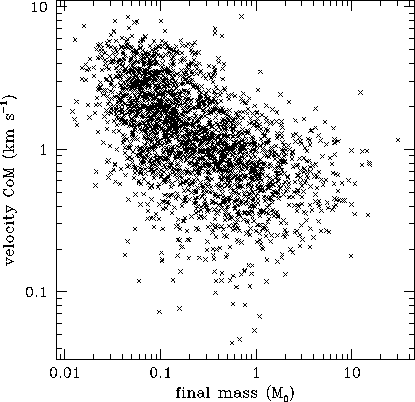
\includegraphics[width=0.7\linewidth]{figures/intro/Bonnell-vrel-mass.pdf}
    \caption[Simulated relative velocity vs. stellar mass in infalling gas filament]{Simulated sink particle velocity relative to the center of mass velocity within $0.25$~pc vs. the final mass of each sink particle. Image credit: \citet{Bonnell-2008}.}
    \label{fig:bonnell}
\end{figure}

The kinematics of young star clusters provide critical insight into their formation conditions, dynamical state, and evolutionary pathways. Specifically, stellar velocity dispersions, bulk motions, velocity gradients, and kinematics substructures can reveal the initial conditions of gravitational fragmentation, gas dynamics, and the virial state of the system. These kinematic states trace the evolutionary stages the clusters have undergone. 

% Velocity dispersion
Velocity dispersion is a key observable in clusters, enabling the inference of their current dynamical state and their formation and evolution pathways. For example, supervirial clusters with velocity dispersion exceeding the virial equilibrium may be dispersing due to rapid gas expulsion, triggered by feedback from massive stars forming from the molecular cloud \citep[e.g.,][]{Goodwin-2006, Offner-2009}. Conversely, subvirial motions can suggest ongoing gravitational collapse, elevated star formation efficiency (SFE), or recent star formation from converging gas flows \citep[e.g.,][]{Kruijssen-2012}. Observations have characterized the virial state of young clusters like the ONC and IC 348 \citep[][]{Cottaar-2015, Theissen-2022}. The SPH simulations by \citet{Offner-2009} and \citet{Grudic-2021} (STARFORGE) show that star clusters initially form in a bound or marginally bound state, depending on the SFE. Low SFE often results in clusters that transition to an unbound state because of mass loss during feedback-driven gas expulsion.

% Substructure
Kinematic substructures, such as anisotropies and localized velocity gradients, trace the formation environment of young star clusters. High-resolution spectroscopic and astrometric surveys have enabled increasingly detailed studies of stellar motions within young clusters. For instance, \citet{Pang-2022} identifies kinematic substructures in open clusters in the solar neighborhood with Gaia data and concludes hierarchical formation through filament dissolution or subgroup mergers. \citet{Furesz-2008} and \citet{Swiggum-2021} also find a velocity gradient in the Orion complex, implying a radial expansion. It is important to differentiate the kinematic substructure inherited from the turbulent molecular cloud and dynamical evolution. As mentioned in the previous section, N-body simulation shows that inherent kinematic features can quickly give way to dynamically induced ones \citep[][]{Allison-2010}.


% Fragmentation in Filaments
Gravitational fragmentation in gas filaments leaves distinct kinematic features on stars formed within these structures. Observations using facilities like ALMA and Herschel have detected coherent velocity structures and gradients across filaments in both low and high-mass star-forming regions, reflecting gas flows feeding the collapsing cores \citep[e.g.,][]{Kirk-2013, Beuther-2015, Kainulainen-2016, Lu-2018}. Velocity dispersion measurements have unveiled that dense gas filaments in star-forming regions grow by accreting surrounding gas until they become unstable, followed by fragmentation and star formation \citep[][]{Arzoumanian-2013}. With SPH simulations, \citet{Bonnell-2008} proposes the formation mechanism of brown dwarfs via gravitational fragmentation in gas filaments infalling towards the cluster center. In this scenario, the high relative velocity and tidal shear of the fast-moving primordial stars preclude them from accreting more material from their surroundings, ultimately leading to the formation of low-mass objects like brown dwarfs. One observable of this mechanism is a negative correlation between the stellar velocity relative to their neighbors and the initial stellar mass, as shown in Figure~\ref{fig:bonnell}. This kinematic signature provides a testable prediction in newly formed star clusters. 



\csuse{phantomsection}
\addcontentsline{toc}{subsection}{Initial Mass Function}%
\subsection*{Initial Mass Function}%

\begin{figure}[htb!]
    \centering
    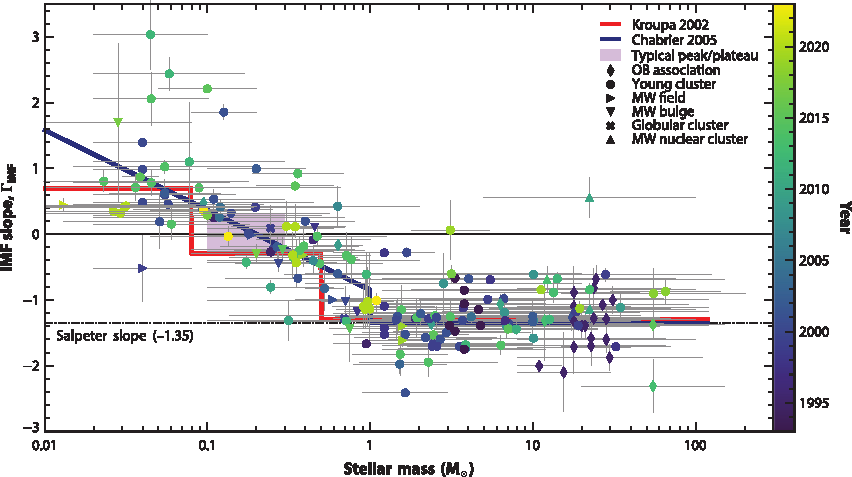
\includegraphics[width=\linewidth]{figures/intro/IMF.pdf}
    \caption[IMF slope measurements as a function of zero-age main sequence stellar mass]{IMF slope measurements as a function of zero-age main sequence stellar mass. Horizontal bars illustrate the mass range over which the slope is measured, and vertical bars show the $\pm 1\sigma$ uncertainties. Image credit: \citet{Hennebelle-2024}.}
    \label{fig:imf-compilation}
\end{figure}

The initial mass function (IMF) describes the distribution of stellar mass at the time of star formation. It is a cornerstone for understanding the formation and evolution of individual stars, clusters, and galaxies. Whether the IMF is universal across various environments remains a critical open question in astrophysics. 

% Observations
The IMF is typically modeled with empirical distributions, such as the power law form proposed by \citet{Salpeter-1955}, the multi-component forms introduced by \citet{Kroupa-2002}, or the log-normal form proposed by \citet{Chabrier-2005}. The Salpeter IMF was derived from massive field stars, while the Kroupa and Chabrier IMFs were constructed using both field stars and young clusters with a peak at around $0.1$--$1.0~M_\odot$. Observational studies of star clusters have tested the universality of the IMF across different environments with limited variations.  For instance, the IMF of the ONC is found to be in good agreement with the canonical IMF for stars $>1~M_\sun$ \citep[e.g.,][]{Hillenbrand-2000, Gennaro-2020}. Additionally, \citet{Weisz-2015} surveys the cluster IMF in the nearby M31 galaxy with the Hubble Space Telescope (HST) and finds that the high-mass IMF appears universal in this environment. Conversely, other measurements detect a top-heavy IMF with an excess of high-mass stars in the most massive clusters in the Milky Way, representing a deviation from the canonical IMF functionals \citep[e.g.,][]{Lu-2013, Schneider-2018, Hosek-2019}. This implies that the cluster formation in extreme conditions may alter the IMF slope. Indeed, \citet{Murray-2009} argues that optically thick massive clusters are born with top-heavy IMFs, since the Jeans mass is observed to increase with cluster mass. Studies have also identified bottom-light IMF with a deficiency in low-mass stars in the ONC, globular clusters in the Milky Way, and massive clusters in the Small and Large Magellanic Cloud \citep[e.g.,][]{DaRio-2012, Baumgardt-2023}. A recent compilation of IMF measurements is shown in Figure~\ref{fig:imf-compilation} \citep[][]{Hennebelle-2024}.

% Simulations
Theoretical studies and numerical simulations suggest that the IMF emerges from a complex suite of physical processes, including but not limited to turbulence, gravity, magnetohydrodynamics, tidal forces, and stellar feedback \citep[][]{Hennebelle-2024}. The high-mass slope of the IMF is most likely determined by gravity and turbulence. For instance, \citet{Padoan-2002} models the IMF as the outcome of turbulent fragmentation, showing that the mass distribution of collapsing cores naturally reproduces the Salpeter slope for stellar masses larger than $1$--$2~M_\sun$. \citet{He-2019} also successfully reproduces the Salpeter IMF with radial-magneto-hydrodynamic simulations including radiation feedback. Simulations have also linked the IMF peak to either the dust opacity \citep[e.g.,][]{Coleman-2020}, or to stellar radiative feedback \citep[e.g.,][]{Krumholz-2016, Cunningham-2018}, offering a possible explanation for the universality of the IMF.


In summary, observations support a universal IMF, but variations in extreme environments highlight the need for further investigation. Simulations have provided valuable insights into the underlying mechanisms, yet challenges remain in fully reconciling theoretical models with observations. Future progress will depend on high-resolution simulations and observations to address the potential biases and reveal the intrinsic IMF.


\csuse{phantomsection}%
\addcontentsline{toc}{section}{Scope of the Dissertation}%
\section*{Scope of the Dissertation}%

\begin{figure}[htb!]
    \centering
    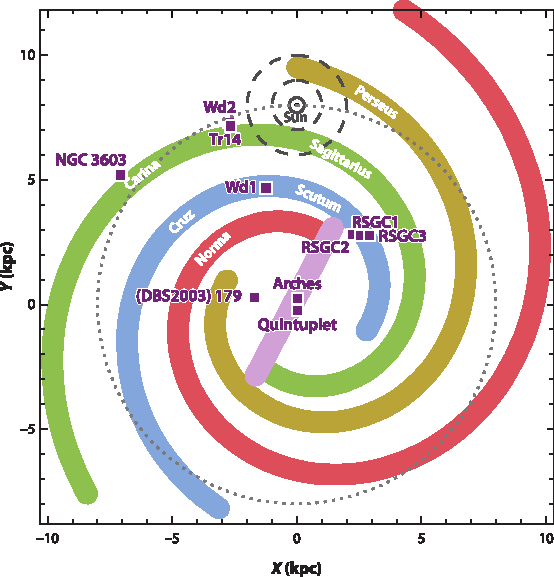
\includegraphics[width=0.7\linewidth]{figures/intro/Milky-Way.pdf}
    \caption[Young Massive Clusters in the Milky Way]{Young massive clusters in the Milky Way, with the spiral arms, location of the Sun, and young star clusters more massive than $\geq 10^4 M_\sun$ identified. The dashed circles indicate $1$~kpc and $2$~kpc from the Sun. Image credit: \citet{PortegiesZwart-2010}.}
    \label{fig:ymc}
\end{figure}

\begin{figure}[htb!]
    \centering
    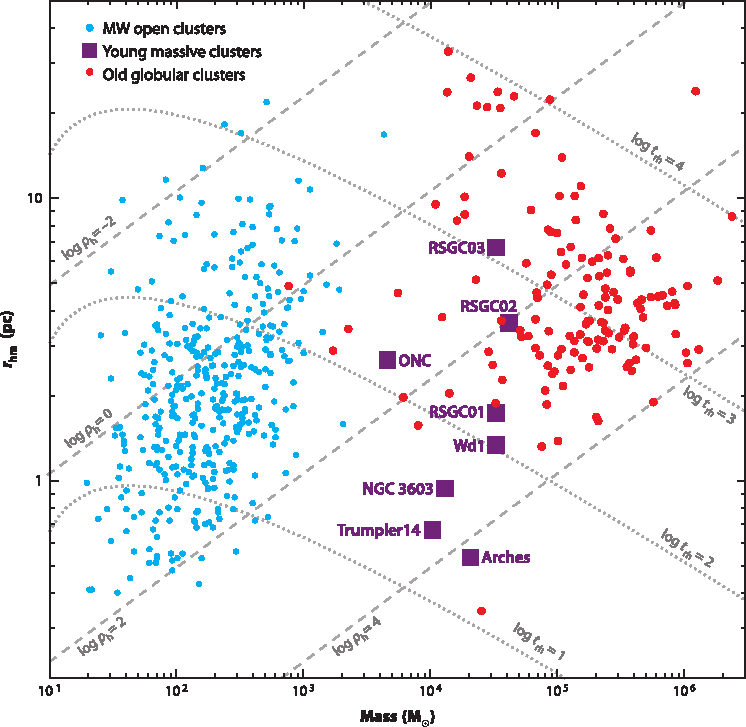
\includegraphics[width=0.7\linewidth]{figures/intro/rhm-mass.pdf}
    \caption[Half-mass-radius vs. cluster mass]{Half-mass-radius vs. cluster mass of Milky Way open clusters, young massive clusters, and old globular clusters. Image credit: \citet{PortegiesZwart-2010}.}
    \label{fig:rhm-mass}
\end{figure}

% Why young massive star clusters?
Despite extensive observational and theoretical efforts, many questions persist regarding the kinematic, structural, environmental, and stellar population details of star formation processes. As discussed, YMCs offer a valuable opportunity to study the star and cluster formation process across the stellar mass range, as their fundamental properties may retain signatures of their origin. Figure~\ref{fig:ymc} shows the spatial distribution of the few resolved YMCs in the Milky Way, with some located in the heart of the Galactic center, whereas others live in the spiral arms. The uniqueness of YMCs can be further illustrated when compared with the other two types of star clusters, namely the open cluster and the globular cluster. Open clusters are a collection of loosely bound stars that are much less massive, whereas globular clusters are evolved, tightly bound conglomeration of stars. Figure~\ref{fig:rhm-mass} shows the half-mass radius against cluster mass for open clusters, YMCs, and globular clusters. Among the three types of clusters, YMC is significantly more massive than the open clusters, resembling the globular cluster population in terms of mass and half-mass radius. However, their younger age sets them apart from the globular clusters, making them a unique population worth studying. While most stars form in small or moderate-sized clusters and associations, the longer lifetimes and extreme physical conditions of massive clusters offer a unique perspective on star formation and cluster evolution \citep[][]{Lada-2003, Bressert-2010, PortegiesZwart-2010, Krumholz-2019}. The ONC and Wd1 are two such nearby YMCs that serve as ideal targets for investigating the mechanisms driving star formation in clustered environments. 


\csuse{phantomsection}%
\addcontentsline{toc}{subsection}{Orion Nebula Cluster: A Nearby Stellar Nursery}%
\subsection*{Orion Nebula Cluster: A Nearby Stellar Nursery}%


\begin{figure}[htb!]
    \centering
    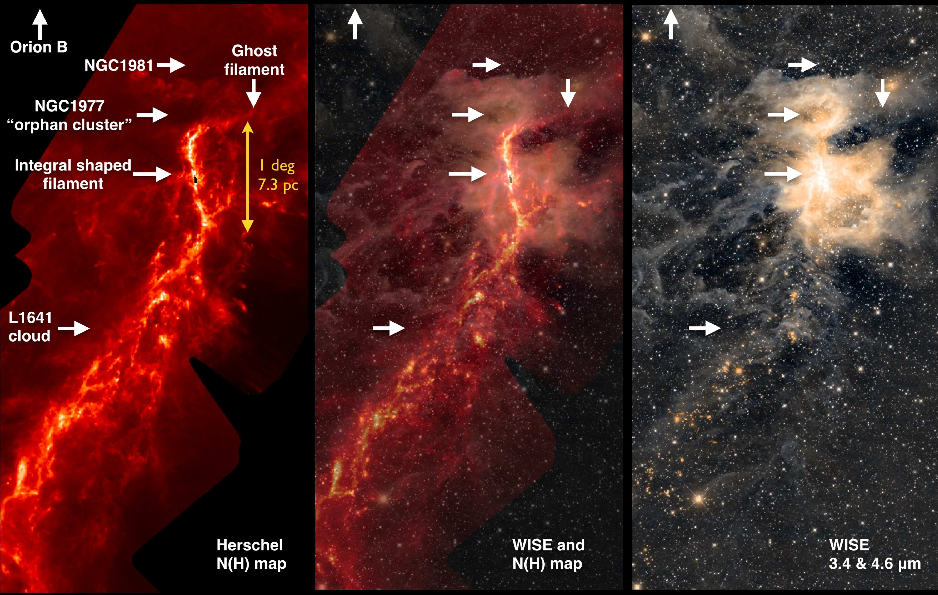
\includegraphics[width=\linewidth]{figures/intro/ISF.pdf}
    \caption[Integral-Shaped Filament]{Spatial configuration of the integral-shaped filament (ISF) and the Orion Nebula Cluster (ONC). \textit{Left}: Herschel column density map of the ISF. \textit{Right}: WISE combined image of the ONC. \textit{Middle}: Combination of the two images. Image credit: \citet{Stutz-2016, Lang-2014}.}
    \label{fig:isf}
\end{figure}

The ONC is one of the most well-studied star-forming regions of the Milky Way and serves as a cornerstone for understanding the processes of star and cluster formation. Located at a distance of approximately ~$400$~pc \citep[][]{Menten-2007, Sandstrom-2007, Kounkel-2018}, the ONC is one of the nearest massive stellar nurseries, hosting active star formation embedded in the molecular cloud and a diverse population of stars spanning the entire mass spectrum. The cluster formed within the larger Orion A molecular cloud complex, which is characterized by filamentary structures \citep[][]{Hacar-2018}. Moreover, the ONC is located within the integral-shaped filament (ISF), a long filament of dense gas with prominent features of ongoing high-mass star formation\citep[][]{Bally-1987}. Figure~\ref{fig:isf} illustrates the spatial configuration of the ISF shown in the Herschel column density map and the ONC shown in the WISE infrared image\citep[][]{Stutz-2016}. Based on radial velocity from the APOGEE survey and Herschel data, \citet{Stutz-2016} observes that the ISF is oscillating and proposes the slingshot star formation mechanism, in which stars form on the filament ridgeline and are ejected as the filament oscillates. Furthermore, \citet{Stutz-2018} identifies dynamical evidence suggesting that star formation in the ONC is regulated by the slingshot motion of the ISF. 

The environmental features imply that the ONC likely inherited dynamical properties from the turbulent and hierarchical parent cloud, making its current kinematics a key tracer of its formation history. For instance, velocity dispersions can reveal whether the cluster is in virial equilibrium or dynamically evolving, and provide a dynamical timescale estimate. In fact, \citet{Stutz-2018} used the timescale comparison with the ISF oscillation timescale as evidence for the slingshot star formation mechanism. Kinematic anisotropies and velocity gradients can reveal whether the cluster is in expansion \citep[][]{Swiggum-2021}. The dependency of stellar velocity and mass can assess brown dwarf formation mechanisms \citep[][]{Bonnell-2008} and whether the ejection of massive stars shaped the IMF in the ONC \citep[][]{Poveda-2005, Kroupa-2018}.

Despite the accessibility and wealth of observational data, many questions about the formation and dynamical evolution of the ONC remain unresolved. Previous observations are plagued by the strong nebulosity and crowding in the cluster center, leaving the central region experiencing the most stellar feedback and gravitational interaction unattended. Therefore, this work aims to resolve the central region of the ONC and study its mass-dependent kinematics with NIRSPAO, a NIR spectrograph with adaptive optics on the Keck Observatory. The detailed results are presented in Chapter~\ref{chapter:onc}.




\csuse{phantomsection}%
\addcontentsline{toc}{subsection}{Westerlund 1: A Massive Stellar Laboratory}%
\subsection*{Westerlund 1: A Massive Stellar Laboratory}%

\begin{figure}[htb!]
    \centering
    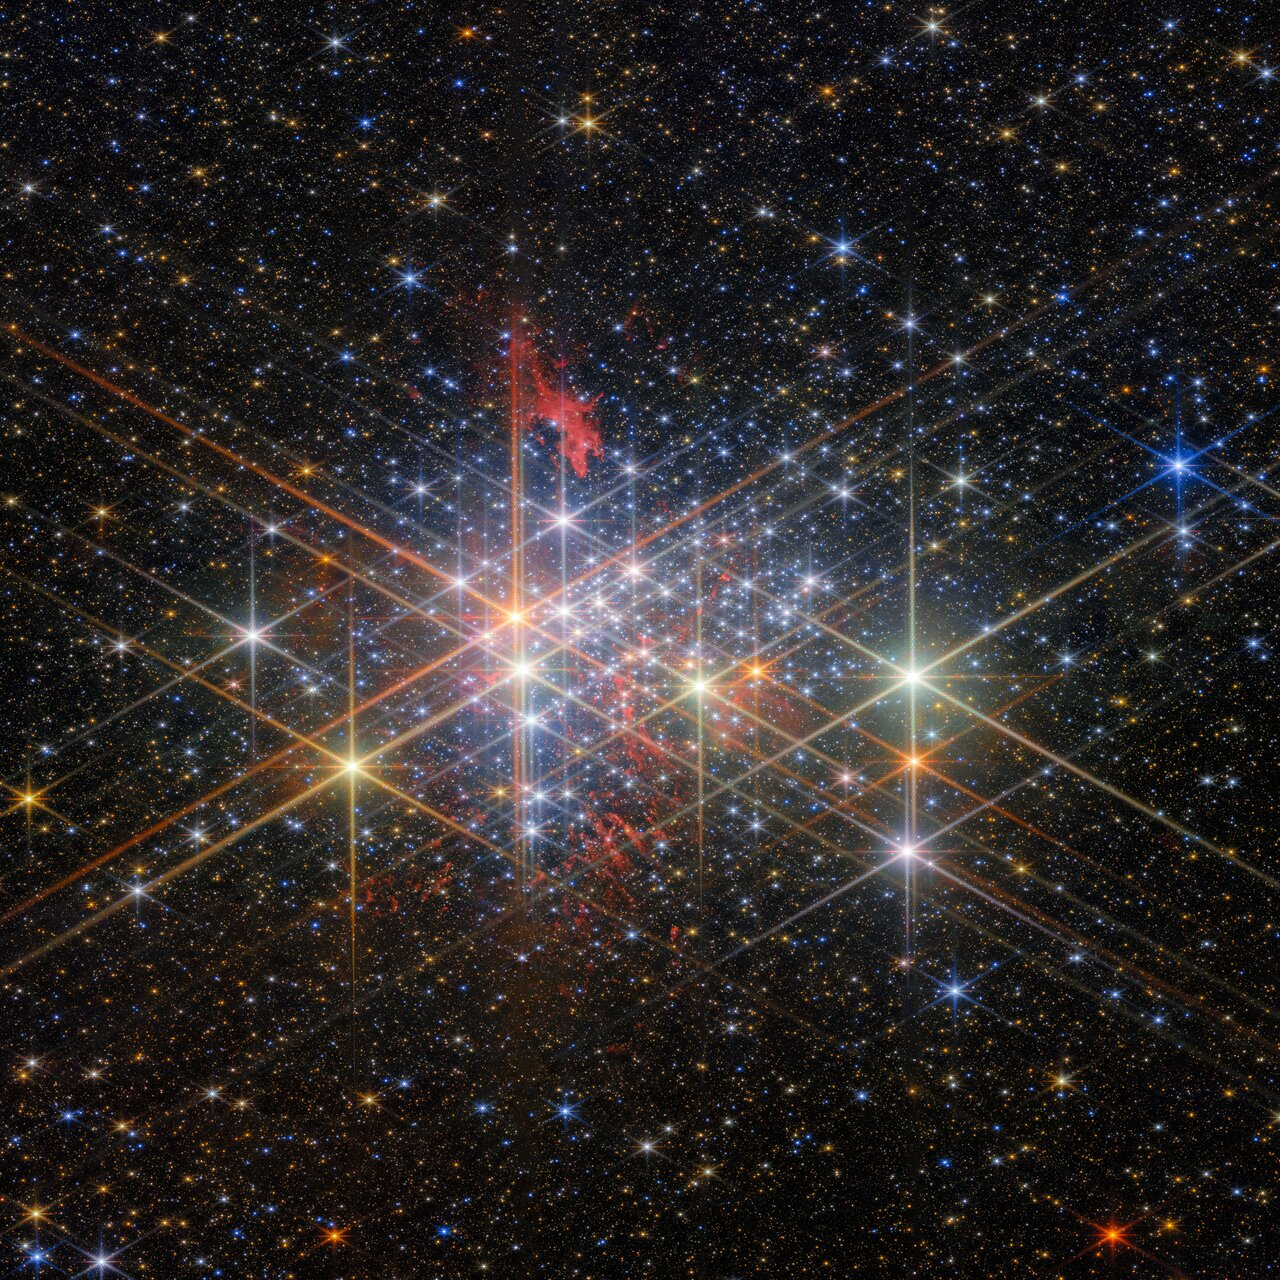
\includegraphics[width=0.6\linewidth]{figures/intro/Westerlund1.jpg}
    \caption[Westerlund 1]{JWST Image of the Westerlund 1}
    \label{fig:wd1-jwst}
\end{figure}
Wd1 is one of the most massive and compact young star clusters in the Milky Way, offering a unique laboratory for studying star formation and evolution in extreme environments. Discovered by \citet{Westerlund-1961}, the cluster is located at a distance $\sim4$~kpc \citep[][]{Negueruela-2022, Rocha-2022} and has an estimated total mass of \num{50000}--\num{100000}~$M_\sun$ \citep[][]{Clark-2005, PortegiesZwart-2010}. Its high stellar density and rich population of stars of various masses make it an exemplary system for exploring the physics of massive star formation, cluster dynamics, and the IMF.

Wd1 is home to a remarkably diverse population of massive stars, spanning a wide range of evolutionary stages. The population includes Wolf-Rayet stars, red and yellow supergiants and hypergiants \citep[][]{Clark-2005, Crowther-2006}, the luminous blue variable Westerlund1-243 \citep[][]{Clark-2004, Ritchie-2009}, and the magnetar CXOU J164710.2-455216 \citep[][]{Muno-2006}. The diversity highlights Wd1 as a snapshot of massive star evolution, where stars can be observed at different evolutionary stages. The rich population also enables constraining the IMF. The higher mass part of the IMF is found to be consistent with the Salpeter IMF and other starburst clusters like the Arches and NGC 3603 \citep[][]{Brandner-2008, Lim-2013}. However, the IMF for the low mass stars remains obscured. Recent observations by the James Webb Space Telescope (JWST) might help constrain the IMF \citep[][]{Guarcello-2025}.

Modeling the IMF requires a detailed picture of the structure and kinematics of the cluster, including the radial density profile, mass segregation, and velocity dispersion. However, observational challenges and limitations exist, hindering our full understanding of the formation and evolution of the cluster. Specifically, Wd1 is known to be located in a region of non-uniform and high extinction with $A_V=10$--$12$ \citep[][]{Damineli-2016, Negueruela-2022} which varies across the cluster. This differential extinction originates from the dark clouds in the Scutum-Crux arm and complicates the reliable determination of the cluster members' color and magnitude. Additionally, the foreground stars in the Scutum-Crux arm can contaminate the proper motion membership determination.
Furthermore, the distance and age uncertainties \citep[][]{Beasor-2021, Aghakhanloo-2021, Negueruela-2022} propagate into stellar mass estimates, introducing systematic errors in the IMF determination. The precise age of Wd1 and whether it exhibits a significant age spread or multi-epoch star formation remain debated. Wd1 is found to be elongated and mass segregated \citep[][]{Gennaro-2011}. The elongation has not been accounted for in modeling its radial density profile, which is critical for accurately constraining the IMF. Also, it is unclear if the mass segregation arises from a primordial origin or from dynamical evolution. 

Current observations of Westerlund 1 provide a wealth of information about its structure, but significant challenges remain. Given the complexity of modeling the structure, dynamical state, age, distance, and mass segregation of the cluster, it is imperative to establish a more comprehensive picture with careful handling of the observational data to mitigate the uncertainties and biases. In light of this, the dissertation presents a detailed modeling of the structure of Wd1 in Chapter~\ref{chapter:wd1}, followed by an analysis of its IMF in Chapter~\ref{chapter:imf}, which builds upon its structural properties.



This dissertation is structured as follows. In Chapter~\ref{chapter:onc}, we investigate the kinematics of the ONC and compare the observed properties with predictions from the hydrodynamical simulation that looks at the origin of low-mass stars and brown dwarfs. In Chapter~\ref{chapter:wd1}, we present detailed modeling of the structure of Wd1 and describe the implications of the structure on the star formation process. Finally, we model the unusual IMF of Wd1 in Chapter~\ref{chapter:imf} and discuss the significance of the deviation from canonical IMF functional forms.

\newpage
% \end{dissertationintroduction}

\chapter{The 3D Kinematics of the Orion Nebula Cluster: Mass-dependent Kinematics of the Inner Cluster}
\label{chapter:onc}
We present the kinematic analysis of $246$ stars within $4\arcmin$ from the center of Orion Nebula Cluster (ONC), the closest massive star cluster with active star formation across the full mass range, which provides valuable insights into the formation and evolution of star clusters on an individual-star basis. High-precision radial velocities and surface temperatures are retrieved from spectra acquired by the NIRSPEC instrument used with adaptive optics (NIRSPAO) on the Keck II 10-m telescope. A three-dimensional kinematic map is then constructed by combining the proper motions previously measured by the Hubble Space Telescope (HST) ACS/WFPC2/WFC3IR and Keck II NIRC2. The measured root-mean-squared velocity dispersion is $2.26\pm0.08~\mathrm{km}\,\mathrm{s}^{-1}$, significantly higher than the virial equilibrium's requirement of $1.73~\mathrm{km}\,\mathrm{s}^{-1}$, suggesting that the ONC core is supervirial, consistent with previous findings. Energy equipartition is not detected in the cluster. Most notably, the velocity of each star relative to its neighbors is found to be negatively correlated with stellar mass.  Low-mass stars moving faster than their surrounding stars in a supervirial cluster suggest that the initial masses of forming stars may be related to their initial kinematic states. Additionally, a clockwise rotation preference is detected. A weak sign of inverse mass segregation is also identified among stars, excluding the Trapezium stars, though it could be a sample bias. Finally, this study reports the discovery of four new candidate spectroscopic binary systems.

\section{Introduction}
\label{onc-sec:intro}
Star clusters are the primary sites for a multitude of star formation processes observed throughout the universe \citep[][]{Lada-2003, Gutermuth-2009}. Studying the formation and evolution of star clusters is therefore of crucial importance to constrain star formation theories. The kinematics of star clusters provide valuable insights into the processes of their formation and evolution. Despite contemporary observational efforts, many of the details regarding formation processes in star clusters remain to be unveiled \citep[e.g.,][]{Krumholz-2014}. A particular challenge has been generating models that successfully explain the formation of low-mass stars ($M < 0.3\,M_\Sun$). Initial models of the competitive accretion process naturally explained the formation of low-mass stars by invoking a natal cluster with similarly-sized cores in which some protostars were cut off from the reservoir of material through violent dynamical interactions \citep[e.g.,][]{Bate-2003}. However, competitive accretion models have difficulties in explaining the existence of protoplanetary disks and wide binary systems amongst the lowest mass stars \citep[e.g.,][]{Burgasser-2007}. More recently, simulations in which low-mass stars form along dense filaments of gas infalling into the forming cluster have more successfully predicted the observed multiplicity and disk properties \citep[e.g.,][]{Bonnell-2008, Kainulainen-2017}. The low-mass stars formed via fragmentation within filaments have high velocities that prevent them from accreting additional material from the environment. The signature of this formation process can potentially be observed in very young, non-relaxed clusters as a negative correlation between velocity and mass.  Therefore, observations that probe the kinematics of stars in young clusters have the potential to shed new light on the origin of low-mass stars.

% Why ONC? Scientific significance + previous limitations
The ONC is an optimal target for the study of the formation and evolution of star clusters, as it is the nearest ($389\pm3$~pc; \citealt{Kounkel-2018}) active massive stellar nursery. At about $2$~Myr \citep[][]{Hillenbrand-1997, Reggiani-2011}, the youth and proximity of the ONC make it ideal for studying the early formation process of a cluster via kinematic measurements, such as radial velocities and proper motions. 

% More previous studies
Despite its proximity to us, kinematic observations are plagued by the nebulosity and crowding in the region, especially towards the center of the ONC, where the Trapezium, a collection of the brightest stars at the heart of the ONC, lies. \citet{Furesz-2008} and \citet{Tobin-2009} conducted a large-scale radial velocity (RV) survey of $1215$ and $1613$ stars in the ONC, respectively, using the multi-fiber echelle spectrograph at the $6.5$-m MMT and Magellan telescopes. \citet{Kounkel-2016} presented a reanalysis of the data in \citet{Tobin-2009} as well as more recent supplementary observations. The Apache Point Observatory Galactic Evolution Experiment (APOGEE; \citealt{Majewski-2017}) spectrograph on the $2.5$-m Sloan Digital Sky Survey (SDSS; \citealt{York-2000}) telescope has also acquired near-infrared high-resolution spectroscopic data towards the broader Orion Complex region \citep[][]{DaRio-2016, DaRio-2017, Kounkel-2018}. However, observations mentioned above have limited coverage near the Trapezium due to its dense, crowded, and highly embedded nature. Most recently, the \textit{Gaia} Data Release 3 (DR3; \citealt{Gaia-2016, GaiaDR3-2023j}) provides more complete coverage in the area with more precise astrometric solutions. However, \textit{Gaia} DR3 lacks the spectroscopic data necessary to infer stellar parameters, such as effective temperature and surface gravity, and as an optical mission, is also plagued by nebulosity. 

% Previous observations + kinematics studies of ONC
\citet[hereafter T22]{Theissen-2022} present a kinematic analysis of $56$ sources within $4\arcmin$ of the ONC center observed by Keck II NIRSPAO and $172$ sources observed by APOGEE. The study concludes that the central region of the ONC is not fully virialized by measuring its intrinsic velocity dispersion (IVD). Moreover, the radial IVD is found to be higher than the tangential component as measured by proper motions from the Hubble Space Telescope (HST) + Keck \citep[][hereafter K19]{Kim-2019}. The work presented here expands the sample size of the sources observed by NIRSPAO and presents further kinematic analysis of the region.


% Unanswered questions
In spite of the observations and studies on the ONC over several decades, many questions remain unanswered regarding the kinematic characteristics and the formation process of this young and dense cluster. For instance, the current virial state of the ONC is unclear. \citet{Hillenbrand-1998} suggests that some portion of the ONC is already bounded, and the cluster will eventually become bound. Velocity dispersion measurements seem to confirm that the ONC is moderately supervirial \citep[e.g.,][]{DaRio-2014, DaRio-2017, Kim-2019, Theissen-2022}. On the other hand, the most recent study on the ONC advocates that the ONC is likely bound, as previous measurements of the virial parameter may be inflated due to ejections in unstable N-body interactions \cite{Kounkel-2022}. N-body simulations can rule out neither possibility \citep[][]{Kroupa-2000, Scally-2005}. Another fundamental question is the formation mechanism of the cluster as a whole. \citet{Kounkel-2022} uses the data from \textit{Gaia} DR3 and identifies a stellar age gradient as a function of their distance from us, implying that the star formation front is propagating into the star cluster, possibly triggered by the shockwave from a supernova in the past. Evidence suggests that the ONC could form in the oscillating integral-shaped filament (ISF), a filamentary gas structure associated with the ONC \citep{Bally-1987}, and recently ejected from the ISF \citep{Stutz-2016, Stutz-2018, Matus-2023}. Such a mechanism of producing protostars is referred to asthe  slingshot scenario.  Moreover, a net infall of young stars along the ISF towards the center is discovered \citep[][]{Kounkel-2022}, consistent with the gravitational fragmentation star formation mechanism \citep[][]{Bonnell-2008}.

In this work, we use the W. M. Keck Observatory to acquire near-infrared (NIR) high-resolution spectra of $91$ sources at the central ONC region, $24$ of which are newly observed after \citetalias{Theissen-2022}. Combined with an updated analysis of $172$ stars observed by APOGEE, astrometric measurements from \textit{Gaia} DR3, and proper motions from the HST + Keck \citepalias{Kim-2019}, a more thorough analysis of the ONC is made possible in this work, pushing the boundary of our understanding of star cluster formation and evolution. 

In Section~\ref{onc-sec:observation}, we introduce the new data from the Keck Observatory and the data reduction processes. Section~\ref{onc-sec:results} presents the results of three-dimensional kinematics, including radial velocity modeled from the spectrum and proper motions measured previously, and the derivation of stellar masses. In Section~\ref{onc-sec:analysis}, we analyze the mass-dependent kinematics of the ONC core, including the virial state, velocity-mass relation, effective temperature offset between NIRSPAO and APOGEE, and preferred proper motion direction. In Section~\ref{onc-sec:binary}, we report the identification of candidate single-lined spectroscopic binaries (SB1): Parenago 1837, V* V1337 Ori, V* 1279 Ori, and Brun 590. Moreover, we simulate the effect of binaries on the velocity dispersion in the section. The implications of our results on kinematic structure, star formation in the ONC are discussed in Section~\ref{onc-sec:discussion}. Mass segregation and binarity in the cluster are also explored in the same section. Lastly, Section~\ref{onc-sec:conclusion} gives a summary of this study and an outlook of our future observation and research plans.

\section{Observation and Data Reduction}
\label{onc-sec:observation}

\begin{figure*}[ht!]
    \centering
    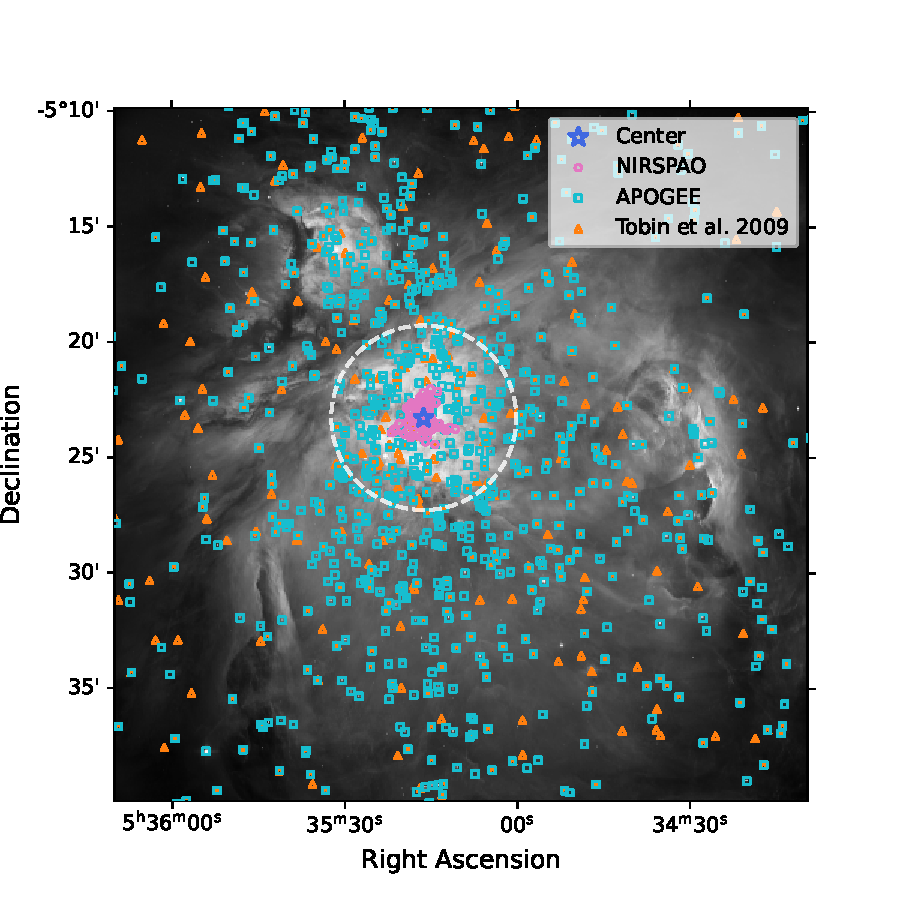
\includegraphics[width=0.496\columnwidth]{figures/chapter1/Skymap_Wide.pdf}
    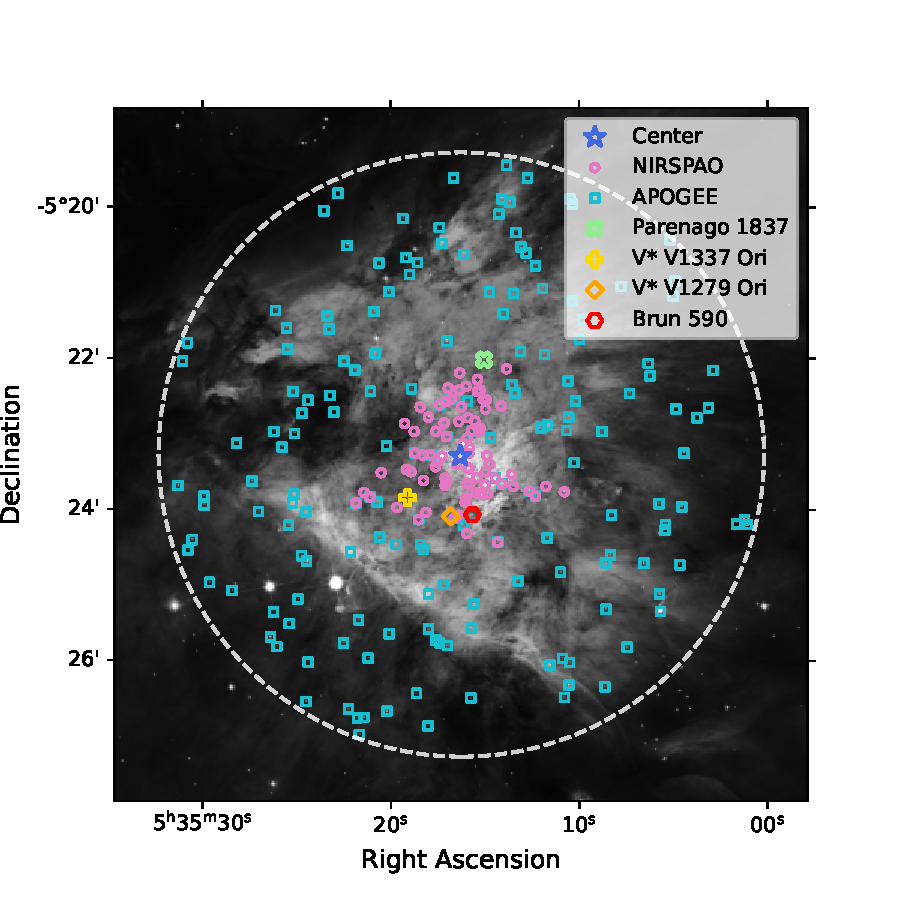
\includegraphics[width=0.496\columnwidth]{figures/chapter1/Skymap_Zoom.pdf}
    \caption[Spatial Distribution of Sources in the Orion Nebula Cluster]{Distribution of sources observed previously and in this study on the background of HST ACS R-band image of the ONC \citep{Robberto-2013}.  \textit{Left:} A wide view of the central $30\arcmin\times30\arcmin$ of the cluster. The $240$ sources observed by NIRSPEC and APOGEE within the circle are selected for analysis in this work. The sources observed by NIRSPAO are marked with magenta circles. Sources observed by APOGEE and by the RV survey in \citet{Tobin-2009} are marked in cyan boxes and amber triangles, respectively. The dashed white circle indicates the $4\arcmin$ radius threshold.  \textit{Right:} A detailed view within the central $4\arcmin$ radius, highlighting the sources considered in this study. The cluster center is labeled as the blue star. Four candidate spectroscopic binary systems identified in this work, namely Parenago 1837, V* V1337 Ori, V* 1279 Ori, and Brun 590, are marked as green plus, yellow cross, amber diamond, and red hexagon, respectively. }
    \label{fig:skymap}
\end{figure*}

\subsection{Sample Selection}
\label{onc-subsec:sample}

Our sample consists of a total of $246$ sources with 2D positions and 3D velocities. $91$ of them are observed by NIRSPAO on Keck II within $2\arcmin$ of the central Trapezium, and $172$ sources are re-analyzed APOGEE sources within $4\arcmin$ of the ONC core, with $17$ sources overlapping.

The NIRSPAO sources were chosen based on their inclusion in the proper motion catalog presented in \citetalias{Kim-2019}, as our goal is to measure the three-dimensional motion of the stars in our sample. The brightness of the sample ranges from $7.4$ to $12.9$ magnitude in K band.  The total size of the sample targeted with new observations of $91$ was primarily driven by observing time constraints from an initial selection of $100$ targets in the central ONC.  The sources were selected to span a range of magnitudes, which roughly corresponds to a range of temperatures and masses.  Since our goal is to assess the kinematic behavior of the lowest mass sources, attention was paid to targeting a sufficient number of faint sources to place statistical constraints on their motion.  A sky map of the sources targeted in this study is illustrated in Figure~\ref{fig:skymap}. Sources observed in this study are pinpointed by magenta circles. 

We supplement the sample observed with an updated analysis of $172$ stars observed by APOGEE within $4\arcmin$ of the center of the ONC \citepalias[][]{Theissen-2022}. APOGEE targets are marked in cyan boxes and the RV survey conducted by \citet{Tobin-2009} and reanalyzed by \citet{Kounkel-2016} are represented as amber triangles in Figure ~\ref{fig:skymap}. The dashed white circle indicates the $4\arcmin$-radius from the center. Throughout this work, we adopted the same location used by \citep[][]{DaRio-2014} as the center of mass of the ONC: $\alpha_{J2000}=05^h35^m16.26^s, \delta_{J2000}=-05^\circ23\arcmin16.4\arcsec$. All $240$ sources in our sample are located within the circle. A zoom-in on this region is shown in the right panel of Figure~\ref{fig:skymap}. As can be seen, previous studies do not have extensive coverage of the central region due to its crowded nature and high level of nebulosity. AO-fed observations in the near-infrared greatly aid in the measurement of individual spectra in this region.

\subsection{Observation}
\label{onc-subsec:observation}

To observe our $91$ targets, we utilized NIRSPEC in conjunction with the Keck II facility laser guide star (LGS) adaptive optics (AO) system \citep[][]{McLean-1998, McLean-2000, vanDam-2006, Wizinowich-2006, Martin-2018}. NIRSPEC is a near-infrared echelle spectrograph on Keck II. The observations were conducted between $2015$ to $2022$. The number of sources observed with NIRSPEC with AO (NIRSPAO) increased from $56$ to $91$ compared to the previous study \citepalias[][]{Theissen-2022}, a $\sim63\%$ increase.  Exposures with NIRSPAO utilize the $0.041\times2.26"$ slit in the the NIRSPEC-7 filter and K-new filter before and after the upgrade, covering the wavelength of $1.839$--$2.630$ and $1.907$--$2.554$, respectively. This wavelength regime covers the carbon monoxide (CO) absorption lines around $2.29$--$2.40~\mu m$, which are present in the spectra of low-mass stars. Moreover, the hydrogen Brackett-$\gamma$ line at $2.166~\mu m$ and the Si, Fe, and Ti lines at $2.18$--$2.19\mu m$ are also within the wavelength range, which helps in inferring the stellar parameters of higher-mass stars. The spectrograph splits the incoming starlight into multiple rows so as to fit in the square-shaped detector, and each row is referred to as an order. In this work, the wavelength coverage of each order in our setup of the detector offset is $2.044$--$2.075~\mu m$ for order $37$, $2.100$--$2.133~\mu m$ for order $36$, $2.162$--$2.193~\mu m$ for order $35$, $2.224$--$2.256~\mu m$ for order $34$, $2.291$--$2.325~\mu m$ for order $33$, and $2.362$--$2.382~\mu m$ for order $32$. The CO lines fall within the range of orders $32-33$, while the Si, Ti, and Fe lines are situated in order $35$ for sources with higher effective temperatures. Therefore, we primarily use orders $32$, $33$, and $35$ to sample the stellar parameters.  The resolution of the spectra is $\mathrm{R}\sim25000$ for data collected before 2019 and $\mathrm{R}\sim35,000$ on or after 2019 as a result of the upgrade on Keck.

While some targets were bright enough to serve as a natural guide star ($R\lesssim15$), the extinction in this region means that most of our sources required LGS.  There are sufficient sources in the region to supply the needed R$\sim$18 tip/tilt guide star requirement within 1' of the target \citep{Wizinowich-2006}.  For the majority of observations, the target was acquired with $\mathrm{PA}=0^\circ$.  However, in some cases there were two sources close enough together to position on the slit simultaneously.  In those instances, we rotated to an appropriate PA to align both stars to the fall on the slit.  

For the majority of the targets, we take four exposures by placing the sources in the slit in an upper-lower-lower-upper sequence, or ABBA dither pattern. In a few cases, the number of frames differs from $4$ due to either loss of target or interruption of observation. HD$37887$, a star of spectral type B9.5IV/V, is used as the calibration star at a similar airmass for telluric wavelength adjustment either before or after a science object is observed.  A log of all NIRSPAO observations, including the dates and the total time of source, is given in Table~\ref{onc-tab:observation}. 

\begin{deluxetable}{lccc}
\tablecaption{Log of NIRSPAO Observations}
\tablewidth{0pt}
\label{onc-tab:observation}
\tablecolumns{4}
\tablehead{
\colhead{HC2000 ID} & \colhead{Date of} & \colhead{No. of} & \colhead{Exp. Time}\\
\colhead{} & \colhead{Obs. (UT)} & \colhead{Frames\tablenotemark{a}} & \colhead{Per Frame (s)}
}
\startdata
 HC2000 322 & 2015 Dec 23 &             4 &       300 \\
 HC2000 296 & 2015 Dec 23 &             4 &      1200 \\
 HC2000 259 & 2015 Dec 23 &             4 &        90 \\
 HC2000 213 & 2015 Dec 23 &             4 &        60 \\
HC2000 306A & 2015 Dec 24 &             4 &       180 \\
$\vdots$ & $\vdots$ & $\vdots$ & $\vdots$\\
% HC2000 306B & 2015 Dec 24 &             4 &       180 \\
% HC2000 291A & 2015 Dec 24 &             4 &       600 \\
% HC2000 291B & 2015 Dec 24 &             4 &       600 \\
%  HC2000 252 & 2015 Dec 24 &             4 &       300 \\
%  HC2000 250 & 2015 Dec 24 &             4 &      1200 \\
%  HC2000 244 & 2015 Dec 24 &             4 &       600 \\
%  HC2000 261 & 2015 Dec 24 &             4 &       900 \\
%  HC2000 248 & 2016 Dec 14 &             4 &       600 \\
%  HC2000 223 & 2016 Dec 14 &             4 &       300 \\
%  HC2000 219 & 2016 Dec 14 &             4 &       600 \\
%  HC2000 324 & 2016 Dec 14 &             3 &      1200 \\
%  HC2000 295 & 2018 Feb 11 &             4 &       450 \\
%  HC2000 313 & 2018 Feb 11 &             4 &       180 \\
%  HC2000 332 & 2018 Feb 11 &             4 &       300 \\
%  HC2000 331 & 2018 Feb 11 &             4 &       450 \\
%  HC2000 337 & 2018 Feb 11 &             4 &        60 \\
%  HC2000 375 & 2018 Feb 11 &             4 &       180 \\
%  HC2000 388 & 2018 Feb 11 &             4 &       120 \\
%  HC2000 425 & 2018 Feb 12 &             4 &        60 \\
%  HC2000 713 & 2018 Feb 12 &             4 &        90 \\
%  HC2000 408 & 2018 Feb 12 &             4 &       450 \\
%  HC2000 410 & 2018 Feb 12 &             4 &       600 \\
%  HC2000 436 & 2018 Feb 12 &             4 &        90 \\
%  HC2000 442 & 2018 Feb 13 &             4 &       450 \\
% HC2000 522A & 2019 Jan 12 &             4 &       450 \\
% HC2000 522B & 2019 Jan 12 &             4 &       450 \\
%  HC2000 145 & 2019 Jan 12 &             4 &       600 \\
%  HC2000 202 & 2019 Jan 12 &             4 &       120 \\
%  HC2000 188 & 2019 Jan 12 &             4 &       600 \\
%  HC2000 302 & 2019 Jan 13 &             4 &       450 \\
%  HC2000 275 & 2019 Jan 13 &             2 &       450 \\
%  HC2000 245 & 2019 Jan 13 &             4 &       180 \\
%  HC2000 258 & 2019 Jan 13 &             4 &       180 \\
%  HC2000 220 & 2019 Jan 13 &             4 &       600 \\
%  HC2000 370 & 2019 Jan 16 &             4 &       180 \\
%  HC2000 389 & 2019 Jan 16 &             4 &       120 \\
%  HC2000 386 & 2019 Jan 16 &             4 &       120 \\
%  HC2000 398 & 2019 Jan 16 &             4 &       120 \\
%  HC2000 413 & 2019 Jan 16 &             4 &       180 \\
%  HC2000 253 & 2019 Jan 16 &             4 &       120 \\
%  HC2000 288 & 2019 Jan 17 &             4 &       450 \\
%  HC2000 420 & 2019 Jan 17 &             4 &       450 \\
%  HC2000 412 & 2019 Jan 17 &             4 &       450 \\
%  HC2000 282 & 2019 Jan 17 &             4 &       450 \\
%  HC2000 217 & 2019 Jan 17 &             4 &       180 \\
%  HC2000 217 & 2020 Jan 18 &             4 &       120 \\
%  HC2000 229 & 2020 Jan 18 &             4 &       450 \\
%  HC2000 228 & 2020 Jan 19 &             4 &       120 \\
%  HC2000 224 & 2020 Jan 19 &             4 &        90 \\
%  HC2000 135 & 2020 Jan 19 &             4 &       180 \\
%  HC2000 440 & 2020 Jan 20 &             4 &       120 \\
%  HC2000 450 & 2020 Jan 20 &             4 &       300 \\
%  HC2000 277 & 2020 Jan 20 &             4 &       300 \\
%  HC2000 204 & 2020 Jan 20 &             4 &       300 \\
%  HC2000 229 & 2020 Jan 20 &             4 &       450 \\
%  HC2000 214 & 2020 Jan 20 &             4 &       450 \\
%  HC2000 215 & 2020 Jan 21 &             4 &       300 \\
%  HC2000 240 & 2020 Jan 21 &             4 &       300 \\
%  HC2000 546 & 2020 Jan 21 &             4 &       300 \\
%  HC2000 504 & 2020 Jan 21 &             4 &       120 \\
%  HC2000 703 & 2020 Jan 21 &             4 &       300 \\
%  HC2000 431 & 2020 Jan 21 &             4 &       120 \\
%  HC2000 229 & 2020 Jan 21 &             3 &       450 \\
%  HC2000 484 & 2021 Feb 01 &             4 &       300 \\
%  HC2000 476 & 2021 Feb 01 &             6 &       300 \\
%  HC2000 546 & 2021 Oct 20 &             4 &       300 \\
%  HC2000 217 & 2021 Oct 20 &             4 &       120 \\
%  HC2000 277 & 2021 Oct 20 &             2 &       600 \\
%  HC2000 435 & 2021 Oct 20 &             3 &       600 \\
%  HC2000 457 & 2022 Jan 18 &             4 &       750 \\
%  HC2000 479 & 2022 Jan 18 &             4 &       900 \\
%  HC2000 490 & 2022 Jan 18 &             4 &       300 \\
%  HC2000 478 & 2022 Jan 18 &             4 &       420 \\
%  HC2000 456 & 2022 Jan 18 &             4 &       900 \\
%  HC2000 170 & 2022 Jan 18 &             4 &       120 \\
%  HC2000 453 & 2022 Jan 19 &             4 &       600 \\
%  HC2000 438 & 2022 Jan 19 &             4 &       300 \\
%  HC2000 530 & 2022 Jan 19 &             4 &       900 \\
%  HC2000 287 & 2022 Jan 19 &             4 &       300 \\
%  HC2000 171 & 2022 Jan 19 &             4 &       120 \\
%  HC2000 238 & 2022 Jan 20 &             4 &       600 \\
%  HC2000 266 & 2022 Jan 20 &             4 &       600 \\
%  HC2000 247 & 2022 Jan 20 &             4 &       300 \\
%  HC2000 172 & 2022 Jan 20 &             4 &       300 \\
%  HC2000 165 & 2022 Jan 20 &             4 &       450 \\
%  HC2000 177 & 2022 Jan 20 &             4 &       420 \\
%  HC2000 163 & 2022 Jan 20 &             3 &       420 \\
\enddata
\tablenotetext{a}{Number of ABBA frames.}
\tablecomments{The first 5 rows are shown here. A machine-readable table is available on the online version of this paper.}
\end{deluxetable}

\subsection{Data Reduction}
\label{onc-subsec:reduction}
NIRSPEC Data Reduction Pipeline (NSDRP)\footnote{\url{https://github.com/Keck-DataReductionPipelines/NIRSPEC-Data-Reduction-Pipeline}} is a pipeline specifically designed for reducing NIRSPEC spectra and is optimized for point sources. In this work, data reduction is conducted using a modified version of the NSDRP\footnote{\url{https://github.com/ctheissen/NIRSPEC-Data-Reduction-Pipeline}}. The modification includes spatial rectification using the object trace instead of the order edge traces, spectral rectification and wavelength calibration using etalon lamps, cosmic-ray cleaning of flats, and bad-pixel cleaning \citep[see][for details]{Hsu-2021-paper, Hsu-2021-code}

The steps to reduce the data for each source are briefly summarized below.
\begin{enumerate}
    \item Median combines the flat frames to generate a master flat frame, which is used to find order edges.
    \item Run the modified NSDRP pipeline to reduce all the frames after trimming the spectra edges.
    \item Perform initial wavelength calibration for each order using etalon or sky lines of the telluric spectra.
\end{enumerate}

The reduced spectra are then forward modeled for stellar parameters, which will be discussed in Section~\ref{onc-subsec:modeling}.


\subsection{Spectral Forward Modeling}
\label{onc-subsec:modeling}
The reduced spectra are coadded and forward-modeled to derive the stellar parameters. Instead of modeling each individual exposure of the same source as in \citetalias{Theissen-2022}, we coadd the spectra before forward-modeling. Compared to modeling each individual exposure, coaddition helps reduce the white noise, enhancing the signal-to-noise ratio (SNR) of the data, and saving computational resources for spectral forward modeling. The specific steps of coaddition are summarized below. First, the flux of each exposure of the same source is scaled to match the median flux of the frame with the highest signal-to-noise ratio (SNR). It is worth mentioning that scaling does not affect the modeling results. The noise is scaled by the same factor. Next, the fluxes of all the exposures on the same target are averaged, weighted by the inverse square of the corresponding noise on a pixel-wise basis. The noise associated with the coadded spectrum is calculated from the uncertainty propagation equation for weighted averaging. The calculation of the weighted-averaged flux and the noise are illustrated in Equation~\ref{eq:flux} and Equation~\ref{eq:noise}, respectively.


\begin{equation}
    \label{eq:flux}
    f_\mathrm{coadd} = \frac{\sum_{i}\left(f_i/\sigma_i^2\right)}{\sum_{i}\left(1/\sigma_i^2\right)}~,
\end{equation}
\begin{equation}
    \label{eq:noise}
    \sigma_\mathrm{coadd}^2 = \sum_{i}\left(\frac{\partial f_\mathrm{coadd}}{\partial f_i}\cdot\sigma_i\right)^2 = \frac{1}{\sum_{i}\left(1/\sigma_i^2\right)}~,
\end{equation}
where $f_\mathrm{coadd}$ and $\sigma_\mathrm{coadd}$ are the coadded flux and noise. $f_i$ and $\sigma_i$ are the flux and noise of the $i$-th frame for a source.

The coadded spectra are then forward modeled using the Spectral Modeling Analysis and RV Tool \citep[SMART\footnote{\url{https://github.com/chihchunhsu/smart}}, ][]{Hsu-2021-code}. We refer the readers to \citet{Hsu-2021-code, Hsu-2021-paper} and \citetalias{Theissen-2022} for a detailed description of the modeling procedure. The steps of modeling spectra are briefly outlined below.

The first step is obtaining a precise absolute wavelength solution. A quadratic polynomial provided by the NSDRP is adopted as the initial wavelength solution\footnote{\url{https://www2.keck.hawaii.edu/koa/nsdrp/documents/NSDRP_Software_Design.pdf}}. A more precise wavelength solution with a systematic uncertainty of $0.058~\mathrm{km}\,\mathrm{s}^{-1}$ is derived by cross-correlating the spectrum of our A-star calibrator, HD $37887$, and a high-resolution reference telluric spectrum \citep[][]{Moehler-2014} in an iterative approach \citepalias{Theissen-2022}. The coefficients of the polynomial are updated in each iteration by fitting the best wavelength shifts for all cross-correlation windows of 100 pixels. The coadded spectrum is calibrated by the telluric frame in order $32$, $33$, and $35$ with the lowest root-mean-square of the residual for the final wavelength solution.

Next, we use the PHOENIX ACES AGSS COND stellar atmospheric models \citep{Husser-2013} to forward-model the coadded stellar spectrum via the Markov chain Monte Carlo (MCMC) method \citep[][]{Butler-1996, Blake-2007, Blake-2008, Blake-2010, Burgasser-2016} realized by the ensemble sampler \textit{emcee} \citep[][]{Foreman-Mackey-2013}. The flux is modeled by the same function of wavelength as in \citetalias{Theissen-2022}. Note that the surface gravity $\log g$ can hardly be constrained from the spectral modeling within the observed wavelength range and is therefore fixed to be $4$, which is the expected value for young, low-mass stars at the age of the ONC and is consistent with other studies \citep[e.g.,][]{Kounkel-2018}. To see how a different $\log g$ might affect the stellar mass estimation based on modeled effective temperature, we conducted a test on a subset of sources spanning across the temperature and SNR range by vigorously changing $\log g$ to $3.5$ and $4.5$, respectively. The majority of the resulting stellar masses remain within $1\sigma$ of the values under the assumption of $\log g=4$. Only a few sources deviate by $2\sigma$ or more due to a trade-off between surface gravity and temperature with the veiling parameter acting as a tuning knob. Overall, the choice of $\log g=4$ is rationalized as the stellar masses largely remain consistent under a relatively wide range of $\log g$. In addition, metallicity is set to be $0$ based on the average value of the ONC \citep[e.g.,][]{D'Orazi-2009}. 

The free parameters we sample and their corresponding limits and initial distribution are summarized in Table~\ref{onc-tab:prior}. The veiling parameter is defined in the same way as in \citetalias{Theissen-2022}.

Each source is sampled with $100$ walkers and $300$ steps using the \texttt{KDEMove}, discarding the first 200 steps, as the walkers typically converge within the first $100$ steps based on the walker plots. We have also verified the consistency of the results by running the MCMC sampler for $500$ steps, thereby ensuring convergence. A fine-tuning sampling with the same number of walkers, steps, and prior distributions follows after removing the pixels where the residual deviates from its median value by more than three standard deviations of itself. The masking removes the remaining bad pixels and cosmic rays from the spectrum that were not rejected by the NSDRP. The final distribution of the last $100$ steps of the $100$ walkers is considered as the posterior distribution. We take the median of the posterior distribution as the measured value for each parameter, and half the difference between the $16$-th and $84$-th percentile, or the $1$--$\sigma$ range for a normal distribution, as the associated uncertainty. Heliocentric RVs are corrected for barycentric motion using the \textit{astropy}
function \texttt{radial\_velocity\_correction}.

In addition to \texttt{emcee}, we also attempted to use another Bayesian inference tool, \linebreak\texttt{PyMultiNest} \citep[][]{PyMultiNest}, to sample the posterior distribution of the stellar parameters, adopting the limits in Table~\ref{onc-tab:prior} as the priors. The built-in multimodal nested sampling algorithm is expected to have a better performance in sampling multimodal distributions, which helps with disentangling potential degenerate distributions between the effective temperature and veiling parameter when either one of them is high. However, as we will show in Section~\ref{onc-subsec:3d velocities}, most of the sources have a low veiling parameter, suppressing the degeneracies. Additionally, we noticed a significant increase in the running time as the number of modeled parameters increases. With $9$--$10$ parameters to sample, \textit{emcee} turns out to be the better option in terms of computation efficiency, which is what we eventually adopted, as \textit{emcee} can also sample multimodal distributions unbiasedly.

Reanalyzed results of the APOGEE samples within $4\arcmin$ of the center of the ONC were performed by \citetalias{Theissen-2022}. The identical sampling procedure that is used on the NIRSPEC data is applied to the APOGEE H-band data to model stellar parameters, including effective temperatures, rotational velocities, and RVs for consistency in methodology. The results conform well with the SDSS/APOGEE results.

\begin{deluxetable}{lcccr}
\tablewidth{0pt}
\tabletypesize{\scriptsize}
\tablecaption{Spectral Forward-Modeling Free Parameters and Their Bounds} \label{onc-tab:prior}
\tablecolumns{5}
\tablehead{
\colhead{Stellar Parameter} & \colhead{Notation} & \colhead{Limit} & \colhead{Initial Distribution\tablenotemark{a}} & \colhead{Unit} %\\
}
\startdata
Effective Temparature & $T_\mathrm{eff}$ & $\left(2300, 7000\right)$ & $U\left(2300, 7000\right)$ & K \\
Rotational Velocity & $v\sin{i}$ & $\left(0, 100\right)$ & $U\left(0, 40\right)$ & $\mathrm{km}\,\mathrm{s}^{-1}$ \\
Radial Velocity (RV) & $V_r$ & $\left(-100,100\right)$ & $U\left(-100, 100\right)$ & $\mathrm{km}\,\mathrm{s}^{-1}$ \\
Airmass & $AM$ & $\left(1, 3\right)$ & $U\left(1, 3\right)$ & ---\\
Precip. Water Vapor & $PWV$ & $\left(0.5, 10\right)$ & $U\left(0.5, 10\right)$ & mm \\
Line Spread Function & $\Delta \nu_\mathrm{inst}$ & $\left(1, 20\right)$ & $U\left(1, 10\right)$ & $\mathrm{km}\,\mathrm{s}^{-1}$ \\
Veiling Param.\tablenotemark{b} & $C_\mathrm{veil}$ & $\left(0, 10^{20}\right)$ & $U\left(0, 10^5\right)$ & ---\\
Noise Factor & $C_\mathrm{noise}$ & $\left(1, 50\right)$ & $U\left(1, 5\right)$ & ---\\
Wavelength Offset & $C_\lambda$ & $\left(-1, 1\right)$ & $U\left(-0.2, 0.2\right)$ & \AA \\
\enddata
\tablenotetext{a}{$U\left(a, b\right)$ denotes uniform distribution between $a$ and $b$.}
\tablenotetext{b}{The veiling parameter is defined in the same way as in \citetalias{Theissen-2022}.}
\end{deluxetable}
For most of the sources, we model orders $32$ and $33$ simultaneously for the stellar parameters. This is where the CO lines reside for low-mass stars. However, this procedure fails for a few high-temperature sources because the spectra in orders $32$ and $33$ are mostly flat without any notable features. Therefore, we modeled Brackett-$\gamma$, silicon, titanium, and iron lines in order $35$ for two high-temperature sources, HC$2000~291$A and HC$2000~337$.

\begin{figure*}[htb!]
    \centering
    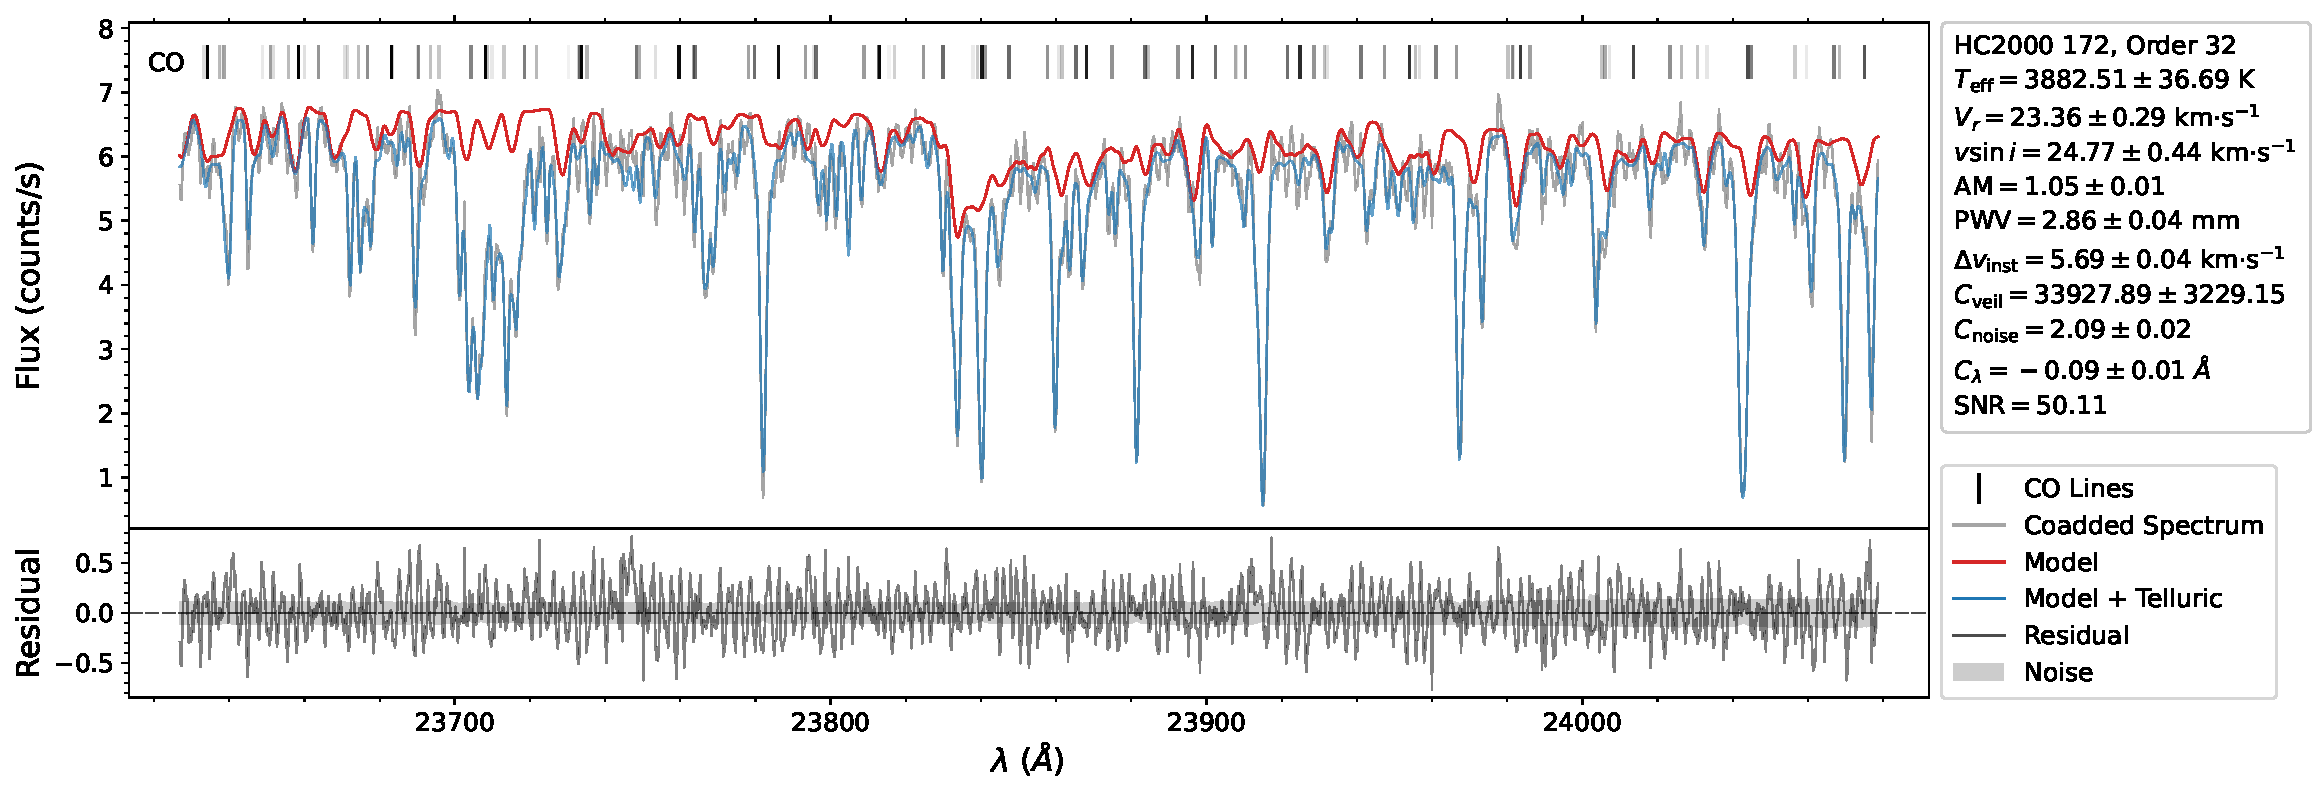
\includegraphics[width=\linewidth]{figures/chapter1/spectrum_modeled_O32.pdf}
    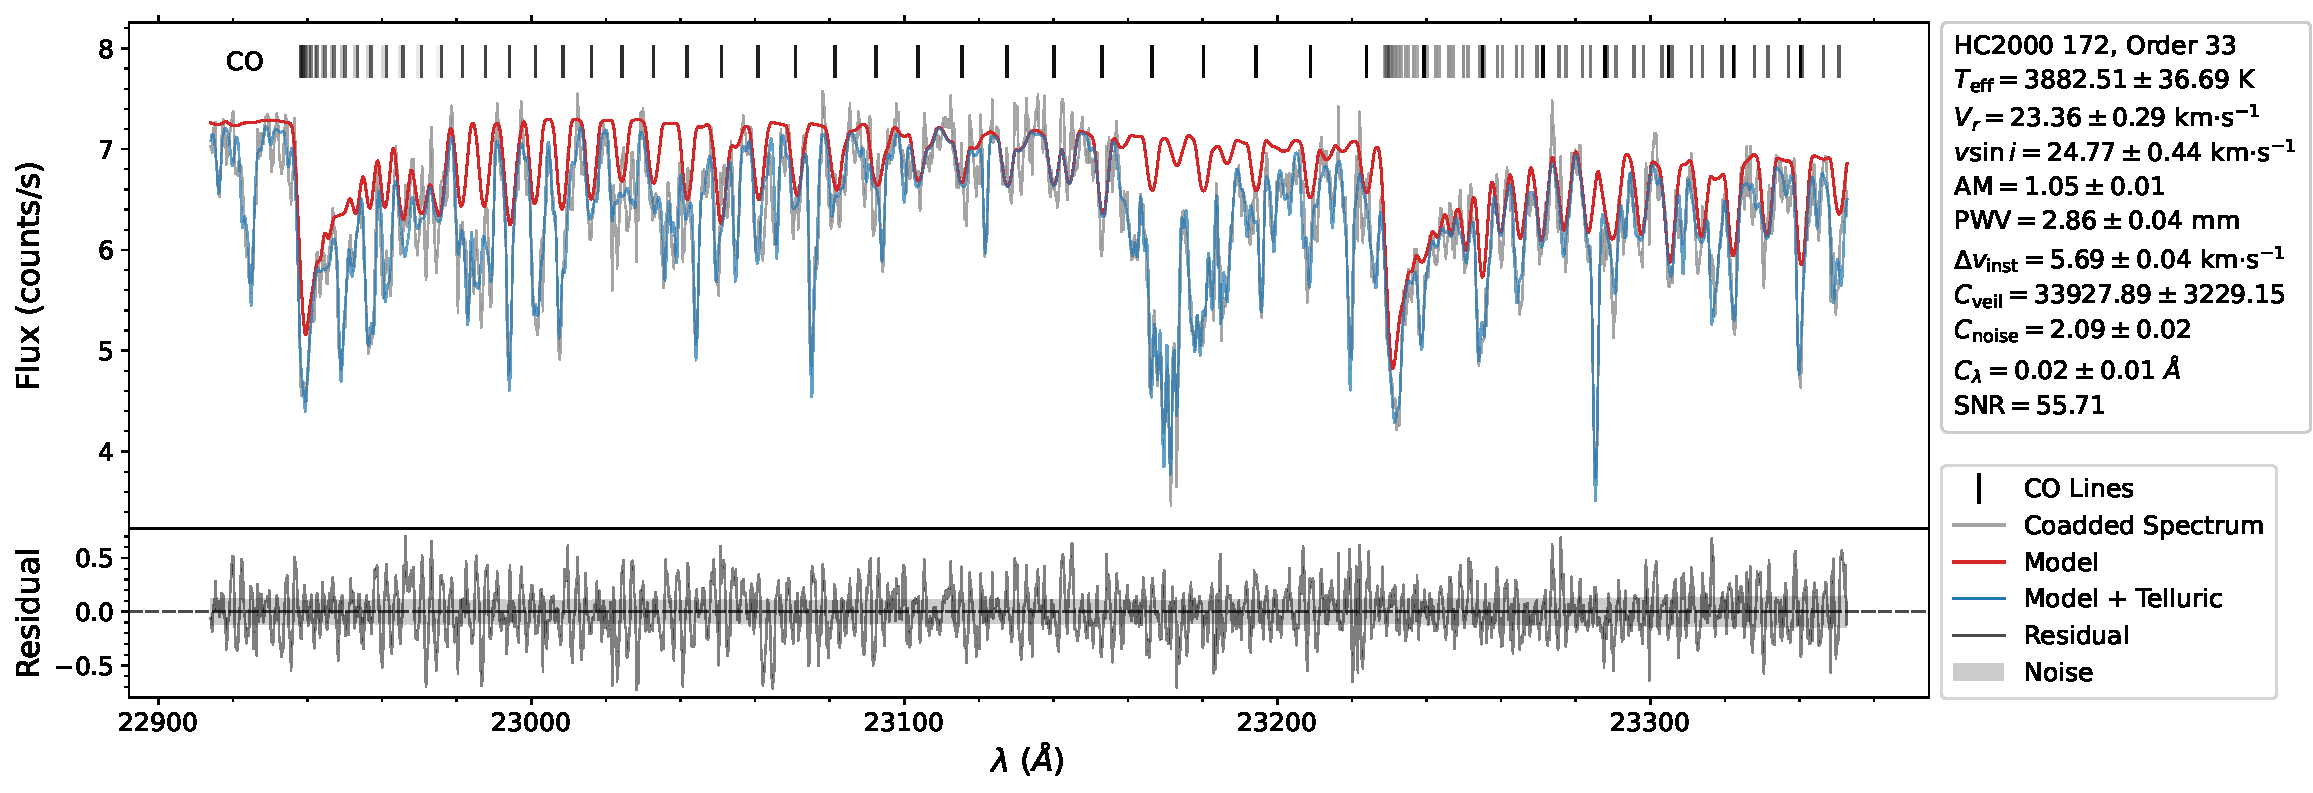
\includegraphics[width=\linewidth]{figures/chapter1/spectrum_modeled_O33.pdf}
    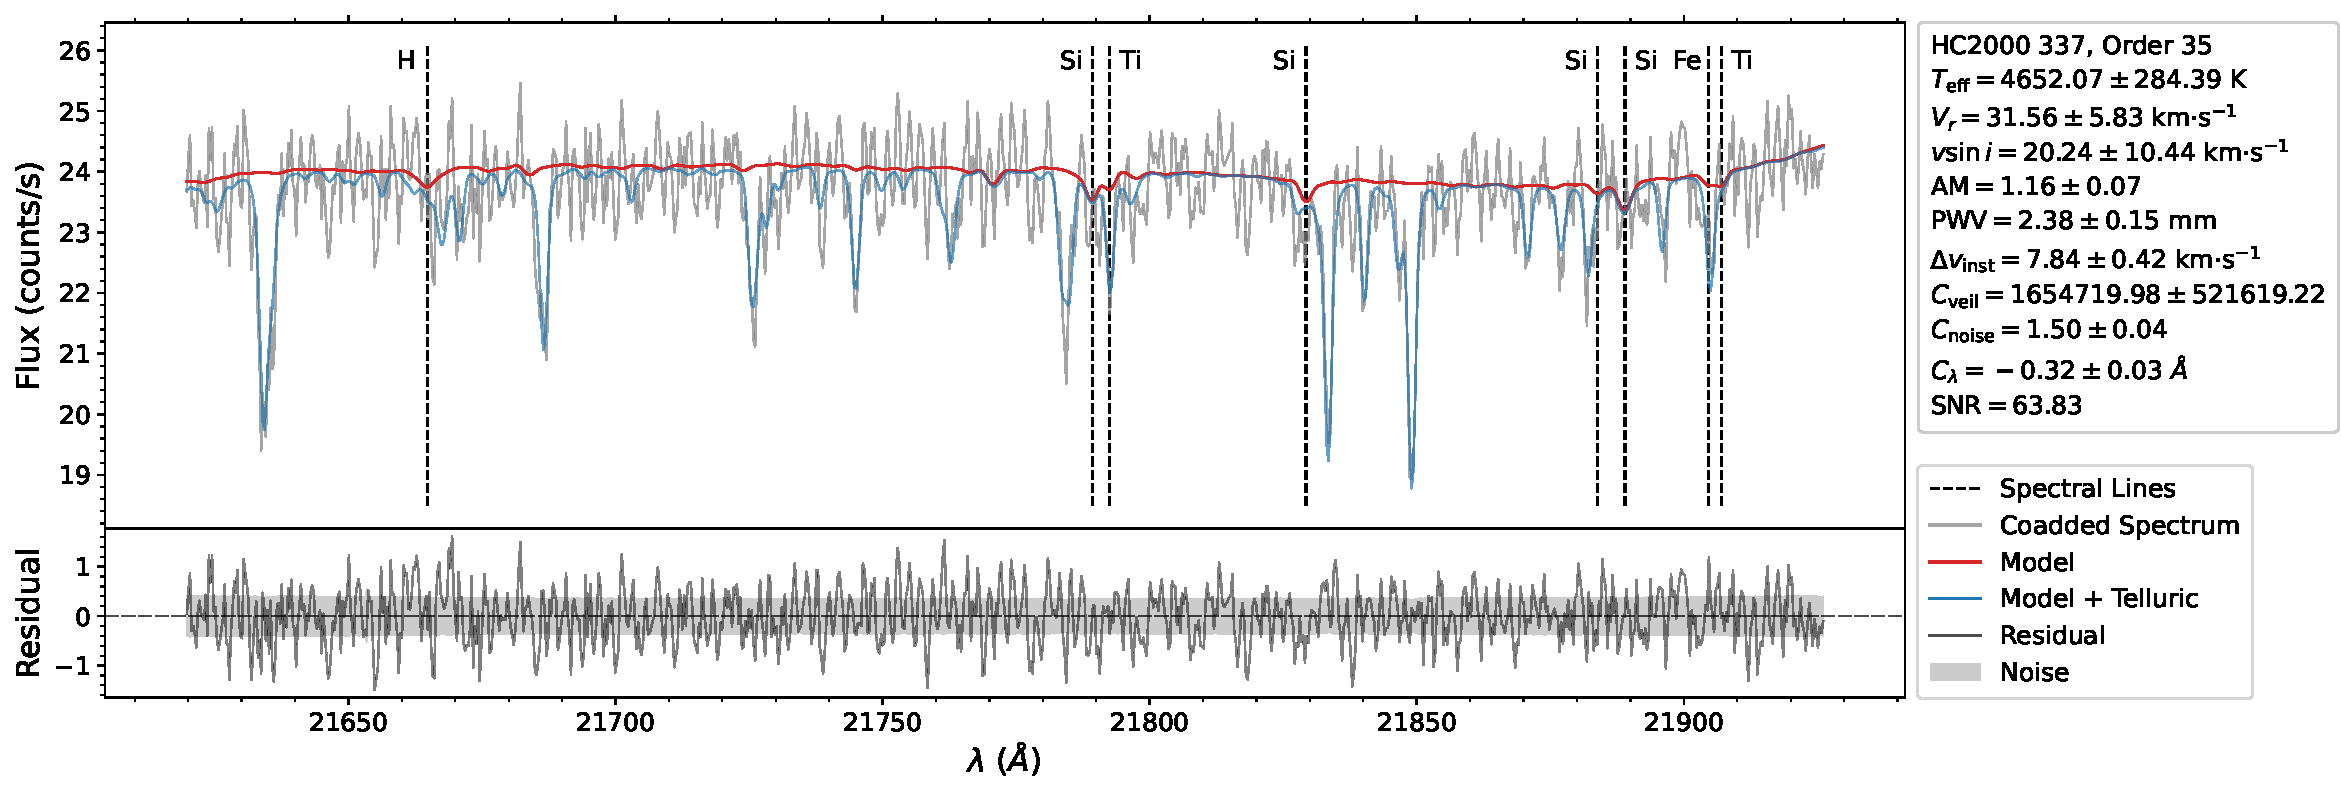
\includegraphics[width=\linewidth]{figures/chapter1/spectrum_modeled_O35.pdf}
    \caption[Examples of observed and modeled NIRSPAO spectra]{Examples of observed and modeled spectra in different orders from NIRSPAO along with atomic and molecular lines. \textit{Top:} HC2000 172 in order $32$; \textit{Middle:} HC2000 172 in order $33$; \textit{Bottom:} HC2000 337 in order $35$. The upper panel in each figure shows the observed spectrum and the model. The vertical lines denote the locations of atomic and molecular spectral lines. The gray line is the normalized observed spectrum flux. The model with and without telluric features are represented as blue and red lines, respectively. The lower panel shows the residual as the black line and the noise as the shaded area. The modeled parameters of each order are labeled beside the corresponding panels. \label{fig:spectrum}}
\end{figure*}


From top to bottom, Figure~\ref{fig:spectrum} shows an example of the spectrum and model in order $32$ and order $33$ for HC2000 172, and order $35$ for HC2000 337, respectively. The top panel in each figure shows the observed spectrum as the gray line, the model as the red line, and the model multiplied by the telluric model as the blue line. CO lines in order $32$ and $33$ are marked on top of the spectra, with their transparency indicating the corresponding lab intensity according to the HITRAN database \footnote{\url{https://www.spectralcalc.com/spectral_browser/db_data.php}}. We implemented a cut of intensity larger than $10^{-25}~\mathrm{cm}\,\mathrm{mol}^{-1}$ for order $32$ for visualization purposes. The intensity is then normalized from $0.05$ to $0.95$ as transparency. Bracket-$\gamma$, silicon, titanium, and iron lines are indicated as vertical dashed lines in the case where we modeled order $35$ in the bottom figure. The bottom panel in each figure shows the residual as the black line and the noise as the shaded area. Typically, the residual is less than $5\%$ of the median flux. According to the modeling results, HC2000 172 is a source with $T_\mathrm{eff}=3882.5\pm36.7~\mathrm{K}$, $\mathrm{RV}=39.25\pm0.29~\mathrm{km}\,\mathrm{s}^{-1}$, and $v\sin{i}=23.36\pm0.44~\mathrm{km}\,\mathrm{s}^{-1}$. The stellar parameters for HC2000 337 are $T_\mathrm{eff}=4652.1\pm284.4~\mathrm{K}$, $v\sin{i}=20.24\pm10.44~\mathrm{km}\, \mathrm{s}^{-1}$, and $\mathrm{RV}=31.56\pm5.83~\mathrm{km}\, \mathrm{s}^{-1}$. The uncertainty of order $35$ fitting results is still significant, even though it is more than $3$ times better than the $32$ and $33$ fits. Caution should be taken when using modeled parameters in order $35$.

Note that the results might be impacted by the fringing in the spectra, which is the primary contributor to the residuals of spectral modeling (\citealt{Hsu-2021-paper}; \citetalias{Theissen-2022}). But it is unlikely to change most of our results.

\section{Results}
\label{onc-sec:results}

\subsection{Three-Dimensional Velocities}
\label{onc-subsec:3d velocities}

\begin{figure}[htb!]
    \centering
    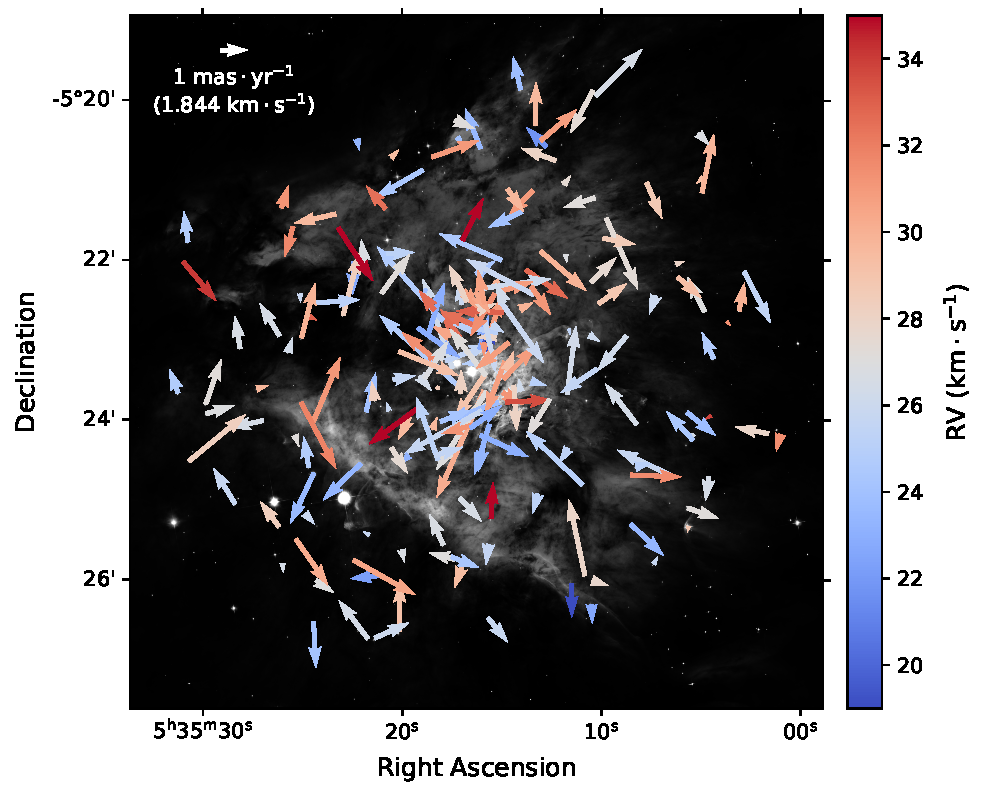
\includegraphics[width=0.8\linewidth]{figures/chapter1/3D_kinematics.pdf}
    \caption[Three-dimensional kinematics of the central ONC]{Three-dimensional kinematics of the central $4\arcmin$ of the ONC. The proper motions are denoted by the direction and length of the arrows, and the radial velocities are illustrated by the color. A $1~\mathrm{mas}\,\mathrm{yr}^{-1}$ key to the quiver plot is shown on the top left, or about $1.844~\mathrm{km}\,\mathrm{s}^{-1}$ assuming a distance of $389$~pc.}
    \label{fig:3d kinematics}
\end{figure}

\begin{figure*}[htb!]
    \centering
    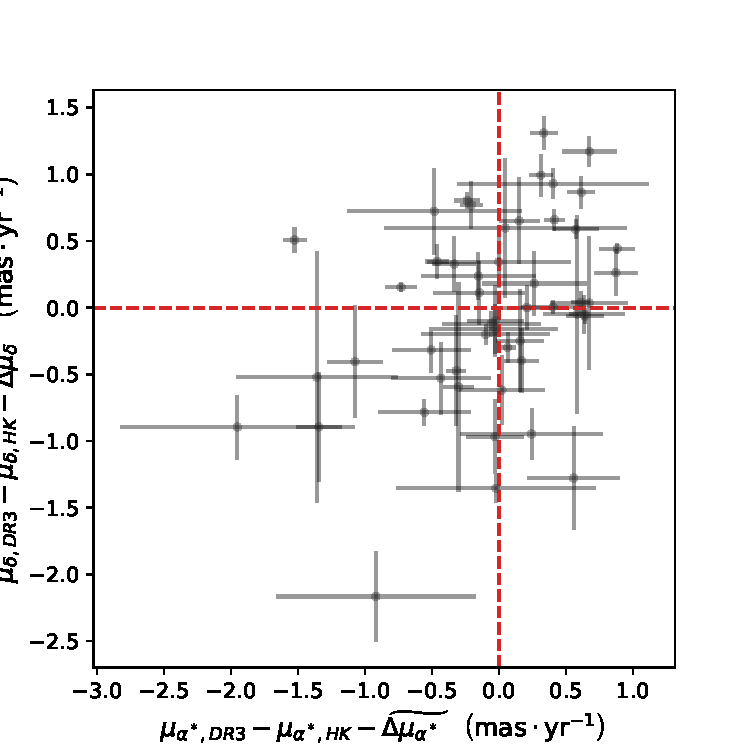
\includegraphics[width=0.496\linewidth]{figures/chapter1/Proper_Motion_Comparison.pdf}
    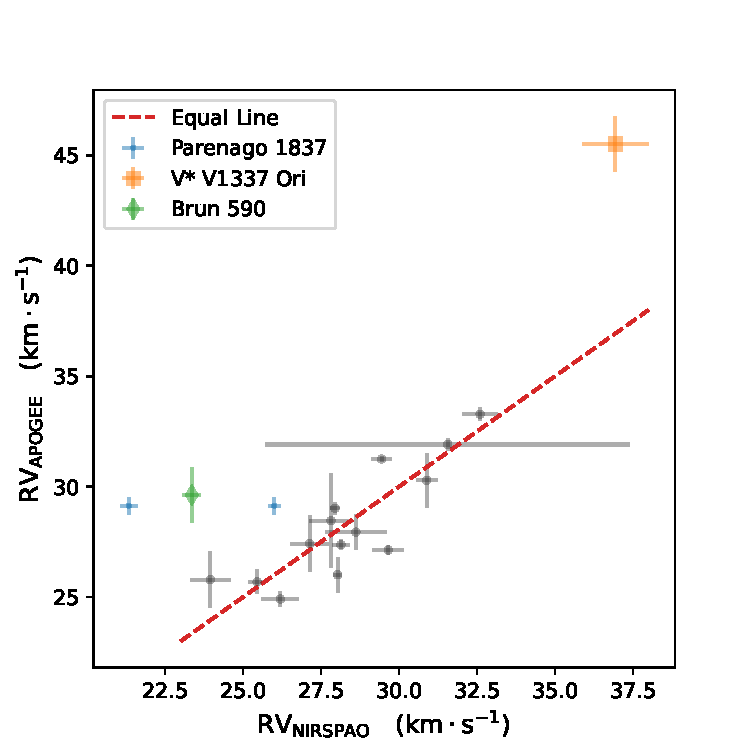
\includegraphics[width=0.496\linewidth]{figures/chapter1/RV_Comparison.pdf}
    \caption[ONC kinematics comparison with previous measurements]{Kinematics comparison with previous measurements. \textit{Left:} Proper motion comparison between \textit{Gaia} DR3 in the absolute frame and HST + Keck in the rest frame. Proper motion in the right ascension and declination are denoted as $\mu_{\alpha^*}$ and $\mu_\delta$, and the measurements from \textit{Gaia} DR3 and \textit{HST} + Keck are denoted as DR3 and HK in the subscript, respectively. In the scope of this work, we transformed the \textit{Gaia} DR3 proper motions into the same reference frame as \textit{HST} + Keck measurements by offsetting the former ones by the average difference between them in both directions. The offsets in right ascension and declination are $\left(\widetilde{\Delta\mu_{\alpha^*}},~\widetilde{\Delta\mu_{\delta}}\right) = \left(1.60,~0.08\right) \mathrm{mas}\,\mathrm{yr}^{-1}$. The red dashed line indicates where the two measurements are equal in RA and DEC directions. \textit{Right:} RV comparison between sources measured with NIRSPAO and APOGEE. The dashed red line indicates the equal line. $3$ of the $4$ candidate binary systems, Parenago 1837, V* V1337 Ori, and Brun 590, are marked in blue dots, amber squares, and green diamonds with errorbars, respectively.}
    \label{fig:kinematics comparison}
\end{figure*}

With the stellar parameters derived from spectral modeling and previous measurements of proper motions and parallaxes, a 3D mass-dependent kinematic map of the ONC core can be constructed. 

% epoch combine
When there are multiple epochs of observations for the same object in the NIRSPAO sources, we take the average of the stellar parameters weighted by the inverse of the square of the associated uncertainties. In the case where there is a match between NIRSPEC and APOGEE sources within $1\arcsec$, the radial velocity derived from the NIRSPAO observation is prioritized over the value from APOGEE since NIRSPAO has a higher resolution($25000$ or $35000$ versus $22500$) and to keep consistency with previous works \citepalias[e.g.,][]{Theissen-2022}.

% cross match with K19 and \textit{Gaia} DR3
The NIRSPAO and APOGEE sources are then cross-matched with both the proper motion catalog measured by the \textit{HST} + Keck \citepalias[][]{Kim-2019}, and \textit{Gaia} DR3 \citep[][]{Gaia-2016, GaiaDR3-2023j} for parallax within a separation of $1\arcsec$ to construct a 3D kinematic map of the ONC core. We retrieved the \textit{Gaia} DR3 data using \texttt{astroquery} \citep[][]{astroquery}. Due to the low quality of astrometric measurements with Gaia induced by the nebulosity and extinction in the ONC region, we adopted the same generous quality cut of \texttt{astrometric\_gof\_al} $ < 16$ and \texttt{photometric\_mean\_g\_mag} $ < 16$ for \textit{Gaia} DR3 sources in the region selected for cross matching as in \citetalias{Kim-2019}. The G magnitude of the cross-matched sources ranges from $7.8$--$16.0$. The proper motion measurements of \textit{HST} + Keck are prioritized over \textit{Gaia} DR3 for the same concern of astrometric measurement quality in the latter.

% quality cuts
To ensure data quality, we applied several constraints on our sample. First, the NIRSPAO and reanalyzed APOGEE sources with a modeled RV uncertainty of no greater than $5~\mathrm{km}\,\mathrm{s}^{-1}$ are selected. $237$ sources out of $246$ remain after the RV constraint is applied. Furthermore, considering our estimated distance from the ONC of $389\pm3$~pc \citep[][]{Kounkel-2018} and the limited accuracy of Gaia astrometric solutions in the region, a generous distance constraint on our sources is imposed with a minimum distance of $300$ pc, a maximum of $500$ pc, and a minimum parallax over error \texttt{parallax\_over\_error} of $5$. $2$ additional source is filtered out in this step, leaving $235$ sources in total. For the remaining sources, we assume the same distance of $389\pm3$~pc \citet{Kounkel-2018} in the following analysis, as only $100$ of the sources have adopted \textit{Gaia} parallax measurements after the aforementioned quality cut and constraints. Moreover, the uncertainties in \textit{Gaia} parallaxes are too large to be accounted for compared to the size of the ONC. The median uncertainty of the parallax after translated into distance, is $8.7$~pc, whereas the radius of the ONC is only about $3.7$~pc.

% 235 total sources
We are left with a total number of $235$ sources after applying both the RV and distance constraints: $85$ NIRSPAO sources within $1.52\arcmin$ from the center; $167$ APOGEE sources within $4\arcmin$; $17$ observed with both instruments. 

% Frame correction
Note that the proper motion measurements of \textit{HST} + Keck are in the rest frame of the ONC, whereas the \textit{Gaia} DR3 is in the absolute frame. We transform the \textit{Gaia} DR3 proper motion into the same reference frame as in \textit{HST} + Keck by offsetting the former values by the average of their differences in each direction. The offsets are $\left(\widetilde{\Delta\mu_{\alpha^*}},~\widetilde{\Delta\mu_{\delta}}\right) = \left(1.60,~0.08\right) \mathrm{mas}\,\mathrm{yr}^{-1}$. 

% 3D kinematics
Figure~\ref{fig:3d kinematics} visualizes the 3D velocities of the sources\footnote{Note that the proper motions of right ascension are incorrectly labeled in the inverse direction in Figure 8 in \citetalias{Theissen-2022}.}
. The proper motions are characterized by the direction and length of the arrows, while RVs are represented by the color code. Sources moving faster away from us with larger RV values are shown in red, and smaller RVs are shown in blue. Discerning the presence of any kinematic structure solely by visual inspection proves challenging. Therefore, a comprehensive analysis will be conducted in Section~\ref{onc-sec:analysis} to explore this further.

% Kinematics comparison
Figure~\ref{fig:kinematics comparison} illustrates the comparison of the kinematics measurements between values adopted in this study and previous observations. The left panel shows the proper motion comparison between \textit{HST} + Keck and \textit{Gaia} DR3. Proper motion in the right ascension and declination are denoted as $\mu_{\alpha^*}$ and $\mu_\delta$, and the measurements from \textit{Gaia} DR3 and \textit{HST} + Keck are denoted as DR3 and HK in the subscript respectively. The source on the bottom left, 2M05351094-0524486 or \textit{Gaia} DR3 3017363547934810112, is the furthest away from consistency because it has a high \texttt{ruwe} of $1.6$, an indication of poor astrometric solution from \textit{Gaia}. In the scope of this work, we only utilize the \textit{Gaia} values if \textit{HST} + Keck RV is not available, as the systematics of the latter are better understood and well accounted for. A similar discussion of comparison between \textit{HST} + Keck and \textit{Gaia} DR2 measurements can be found in \citetalias{Kim-2019}. The right panel shows the RV comparison of the matched sources between NIRSPAO and APOGEE. The binary candidates are marked in different colors.

% Comparison with T22
The comparison between the forward-modeled parameters of NIRSPAO sources in this work and \citetalias{Theissen-2022} is illustrated in Figure~\ref{fig:compare T22}. Most of the sources have consistent effective temperatures and RVs. The median absolute difference in effective temperature is $29$~K, and the maximum difference is $641$~K, mostly within the error bars of \citetalias{Theissen-2022}. Parenago 1837 accounts for the largest well-constrained RV difference, which is shown in blue. Compared with \citetalias{Theissen-2022}, most of the new sources in this work have low veiling parameters, indicating less dust absorption, which helps disentangle the aforementioned degeneracy between the effective temperatures and veiling parameters, yielding more confidently constrained modeled stellar parameters.


\subsection{Stellar Mass Derivation}
\label{onc-subsec:mass}

With the effective temperature obtained from the forward modeling, stellar mass can be interpolated from evolutionary models. We assume an identical age of $2\pm1$ Myr for all sources in the scope of this work. The reason is twofold. First, the estimated age of the ONC is well-established at around $2$ Myr \citep[][]{Hillenbrand-1997, Reggiani-2011}. Second, the stellar age is only used for the interpolation of stellar mass. Even if we allow a relatively large uncertainty of $50\%$ in the stellar age, it does not affect the mass interpolation for low-mass stars, which are the majority of our sample. Figure~\ref{fig:mist model} illustrates the stellar mass as a function of the effective temperature for stars of different ages under the MIST stellar evolutionary model. Degeneracies do not become significant until the effective temperature exceeds $4500$ K. Indeed, $94\%$ of our sources have a lower effective temperature than $4500$ K. Therefore, it is justified to assume a stellar age of $2\pm1$ Myr for all sources for the purpose of mass interpolation.

Four different stellar evolutionary models are used for the mass interpolation: the MESA Isochrones \& Stellar Tracks (MIST; \citealt{Dotter-2016, Choi-2016}), the BHAC15 model\citep[][]{Baraffe-2015}, non-magnetic isochrones in \citet{Feiden-2016}, and the \citet{Palla-1999} model. The stellar mass is interpolated using the effective temperature under the assumption of a uniform $2\pm1$ Myr age and $0$ metallicity. We calculate the uncertainty in the interpolated mass by taking half of the difference between the highest and lowest mass in the model grid when varying the effective temperature and stellar age within their associated uncertainties, respectively. 

Figure~\ref{fig:mass comparison} illustrates the mass comparison using all four models as well as the values from \citet{Hillenbrand-1997}, which uses the evolutionary model by \citet{D'Antona-1994}. Most of the temperature-based interpolated masses agree with one another. However, there is a discrepancy between the masses in \citet{Hillenbrand-1997} and our interpolated values. Effective temperature and luminosity are used to determine the stellar mass in their study. The high nebulosity and reddening in the ONC area make a reliable determination of the luminosity challenging. The use of more recent stellar evolutionary models and age instead of luminosity as the proxy to infer the stellar masses in this work accounts for the difference.

We present the derived parameters from modeling for all sources in our sample in Table~\ref{onc-tab:results}, including RV, $v\sin i$, temperature, and mass.

\section{Mass-Dependent Kinematics Analysis of the Central ONC}
\label{onc-sec:analysis}

\subsection{Virial State and Energy Equipartition}
\label{onc-subsec:virial}

The ONC was previously found to be supervirial (\citealt{Scally-2005, DaRio-2014, Kounkel-2018}; \citetalias{Theissen-2022}). In this study, we revisit this assertion for the central ONC with a larger and denser sample than before in this region.

\citet{DaRio-2014} derived the theoretical velocity dispersion for the ONC based on the stellar and gas density profiles within $3$ pc of the Trapezium center. The stellar density is 
\begin{equation}
    \label{eq:star}
    \rho_\mathrm{star}\simeq70M_\odot\, \mathrm{pc}^{-3} \left(\frac{r}{pc}\right)^{-2.2},
\end{equation}

\noindent where $r$ is the radius from the center of the ONC, and the gas density is

\begin{equation}
    \label{eq:gas}
    \rho_\mathrm{gas}\simeq22M_\odot \, \mathrm{pc}^{-3}.
\end{equation}

\noindent According to the virial theorem, the velocity dispersion $\sigma$ at a certain radius $r$ is related to the enclosed mass within if in virial equilibrium as in Equation~\ref{eq:virial theorem}
\begin{equation}
    \label{eq:virial theorem}
    \frac{GM}{r^2} = 2\sigma^2.
\end{equation}

\noindent Substituting the mass with the integral of the density over the $4$~arcmin (about $0.45$~pc) radius, the dependence of velocity dispersion on the radius can be explicitly derived as in Equation~\ref{eq:vdisp equation}:

\begin{equation}
    \label{eq:vdisp equation}
    \sigma\left(r\right) = \left[\frac{1}{37}\left(\frac{70}{0.8}\left(\frac{r}{pc}\right)^{-0.2} + \frac{22}{3}\left(\frac{r}{pc}\right)^2\right)\right]^{1/2} \mathrm{km}\,\mathrm{s}^{-1}~.
\end{equation}

\begin{figure*}[htb!]
    \centering
    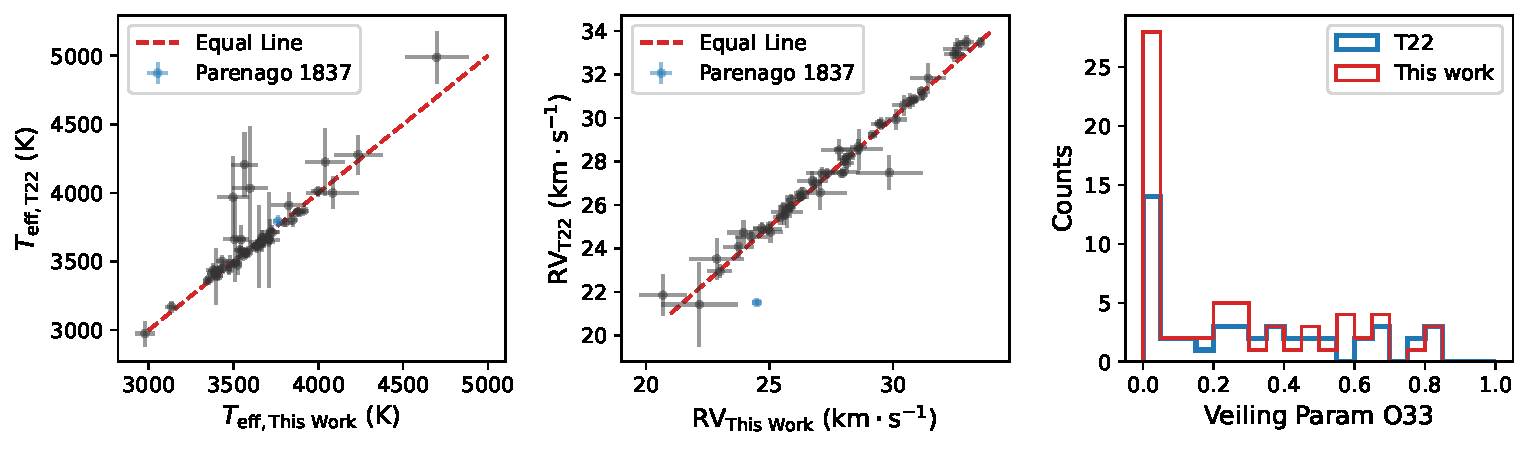
\includegraphics[width=\linewidth]{figures/chapter1/compare_T22.pdf}
    \caption[Effective temperature and radial velocity comparison]{Comparison between the forward-modeled parameters in this work and \citetalias{Theissen-2022}. \textit{Left:} Comparison of effective temperature. The median absolute difference is $29$~K, with a maximum difference of $641$~K. The standard deviation of the differences is $134$~K. \textit{Middle:} Comparison of RV. Note that the most different one shown in blue is the identified binary Parenago 1837. Apart from the binary, the median absolute difference in RV is $0.22~\mathrm{km}\,\mathrm{s}^{-1}$, and the standard deviation of the difference itself is $0.49~\mathrm{km}\,\mathrm{s}^{-1}$. \textit{Right:} Comparison of the distribution of the veiling parameter of order 33.}
    \label{fig:compare T22}
\end{figure*}

\begin{figure}[htb!]
    \centering
    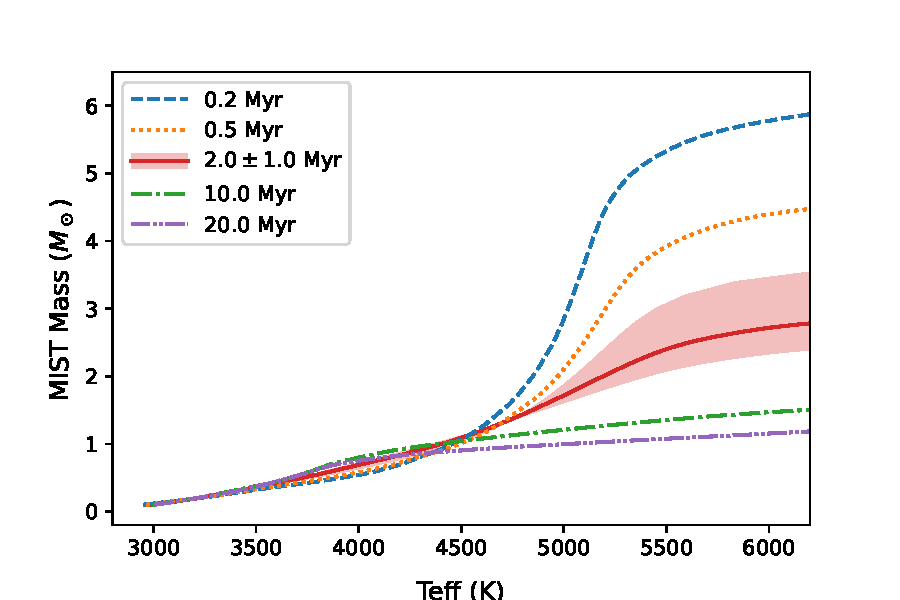
\includegraphics[width=\linewidth]{figures/chapter1/MIST_Evolutionary_Models.pdf}
    \caption[Mass-temperature relation in MIST model]{Mass-temperature relation for stars of different ages using the MIST stellar evolutionary model. The red line and shaded area show the model for stars of age $2\pm1$ Myr, which is our assumption for stellar age in this work.}
    \label{fig:mist model}
\end{figure}

\begin{figure}[htb!]
    \centering
    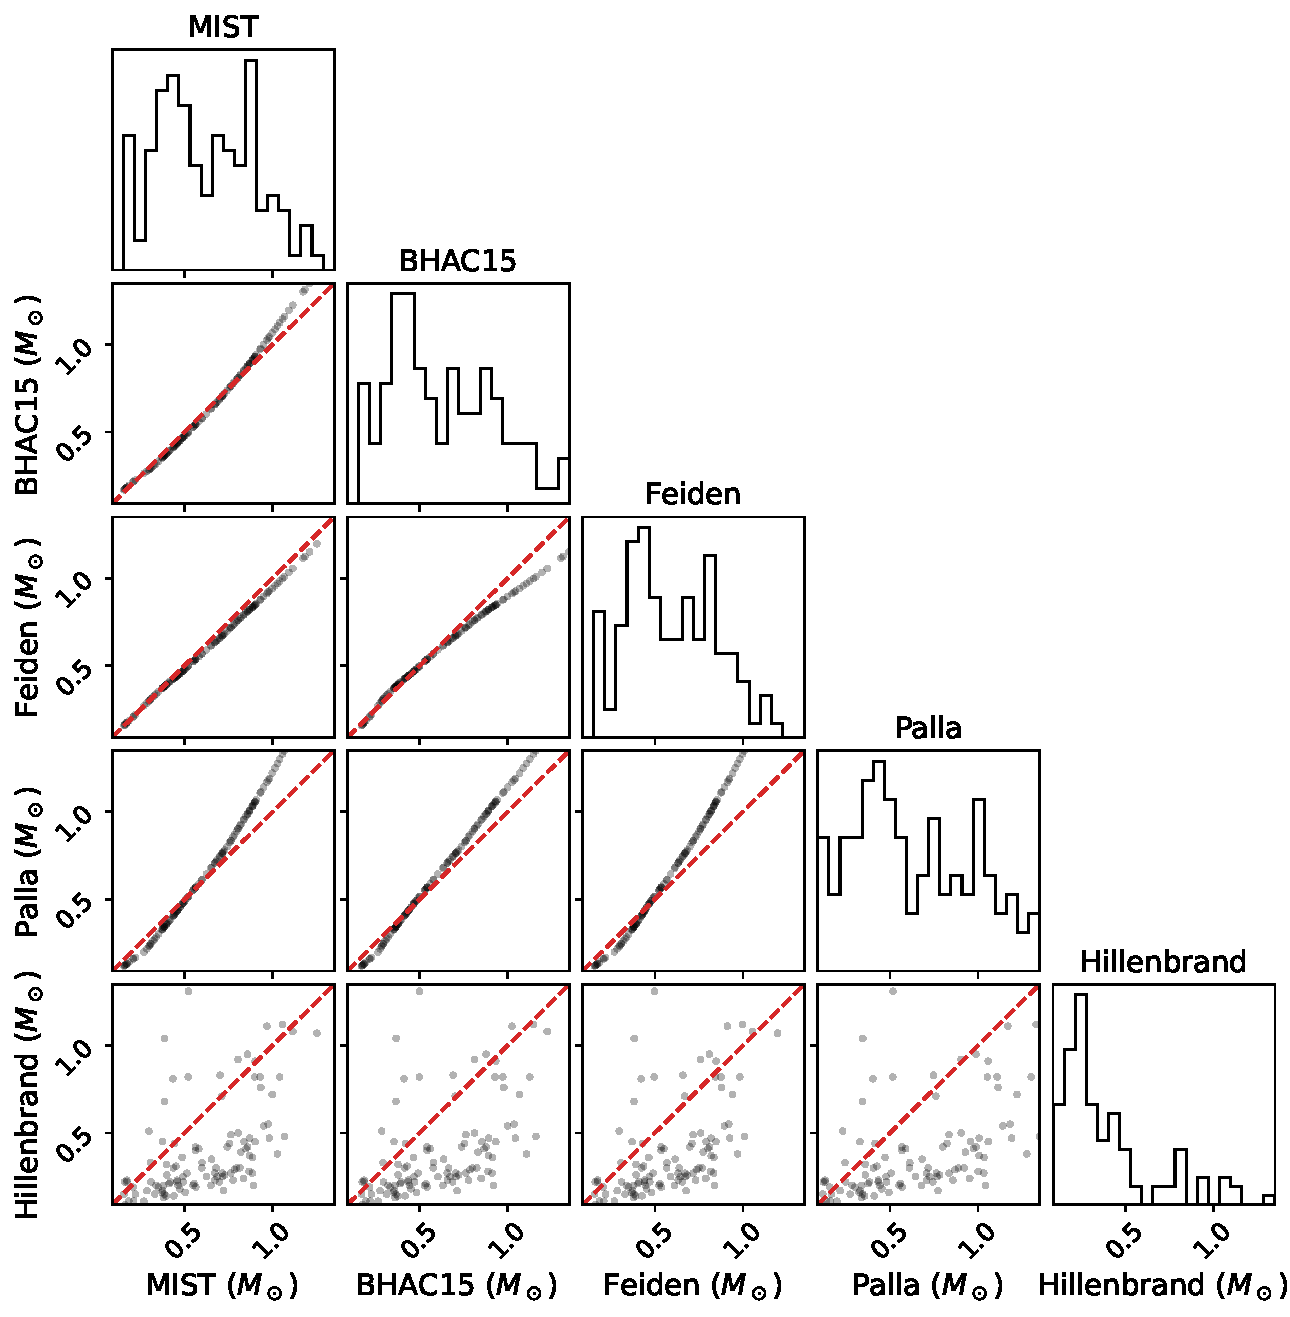
\includegraphics[width=\linewidth]{figures/chapter1/mass_comparison.pdf}
    \caption[Comparison of interpolated stellar mass with different stellar evolutionary models]{Interpolated stellar mass using four different stellar evolutionary models: MIST, BHAC15, Feiden, and Palla.  Also shown are the values in \citet{Hillenbrand-1997} which uses the evolutionary tracks in \citet{D'Antona-1994} for stars less than $3 M_\odot$.}
    \label{fig:mass comparison}
\end{figure}

We measure the velocity dispersion of our sources, assuming there is an intrinsic velocity dispersion along with a measurement uncertainty. That is, the velocity of the $i$-th source in each direction can be parameterized as $v_{(\alpha, \delta, r)_i} \pm \sqrt{\sigma_{{(\alpha, \delta, r)}_i}^2 + \epsilon_{{(\alpha, \delta, r)}_i}^2}$, where $\sigma_{{(\alpha, \delta, r)}_i}$ denotes the intrinsic velocity dispersion and $\epsilon_{{(\alpha, \delta, r)}_i}$ denotes the measurement uncertainty. Note that in this analysis, we excluded sources whose radial velocity deviates more than $3\sigma$ from the mean value to avoid the effects of extreme values, which may be caused by the signal-to-noise ratio of the data or unresolved binaries. The accepted radial velocity range is $27.57\pm13.21~\mathrm{km}\,\mathrm{s}^{-1}$, leaving out $5$ sources with $2$ being Trapezium stars, which are multiple systems. MCMC forward-modeling is adopted to sample the intrinsic velocity dispersion. The same algorithm is used as in \citetalias{Theissen-2022} for the modeling. We directly report our updated values below. The velocity dispersion in each direction and the one-dimensional (1D) velocity dispersion, defined as $\sigma_\mathrm{1D_{3D}}=\sqrt{\left(\sigma_\mathrm{RA}^2 + \sigma_\mathrm{DEC}^2 + \sigma_\mathrm{RV}^2\right)/3}$, are listed in Equation~\ref{eq:vdisp measurements}:
\begin{align} \label{eq:vdisp measurements}
    \sigma_\mathrm{RA} = 1.73 \pm 0.09~\mathrm{km}\,\mathrm{s}^{-1}, \nonumber \\
    \sigma_\mathrm{DEC} = 2.03 \pm 0.11~\mathrm{km}\,\mathrm{s}^{-1}, \nonumber \\
    \sigma_\mathrm{RV} = 2.87 \pm 0.16~\mathrm{km}\,\mathrm{s}^{-1}, \nonumber \\
    \sigma_\mathrm{1D_{3D}} = 2.26 \pm 0.08~\mathrm{km}\,\mathrm{s}^{-1}.
\end{align}
\citet{DaRio-2014} estimate a RMS velocity dispersion in each direction of $1.73$ km/s if the ONC is in virial equilibrium. Our result of $2.26$ km/s is clearly larger than this value (by over $6$--$\sigma$) and indicates that the ONC is supervirial with a virial ratio (kinetic over potential energy) of $q=\left(\sigma_\mathrm{1D_{3D}}/\sigma_\mathrm{equilibrium}\right)^2/2\sim0.85$, consistent with the value in \citet{DaRio-2014}. Therefore, we reconfirm that the ONC center is supervirial.

Figure~\ref{fig:vdisp} shows the velocity dispersion as a function of separation from the center of the cluster. To mitigate against any potential bias in the result due to different ways of binning, the sources are binned equally spaced, i.e., with an identical bin width, and equally grouped, i.e., with an almost identical number of sources in each bin. In Figure~\ref{fig:vdisp}, the left column shows the case of equally spaced bins, while the right column shows equally grouped bins. From top to bottom, each row shows the 1D root-mean-squared velocity dispersion, proper motion component, and radial velocity component, respectively. It can be seen from the middle row in Figure~\ref{fig:vdisp} that the proper motion component is consistent with the virial equilibrium model. However, the radial velocity dispersion (bottom row) is higher than the requirement of virial equilibrium. Consequently, the 1D velocity dispersion of the ONC core sits right above the theoretical prediction of virial equilibrium regardless of the binning method, confirming the result that the ONC is not fully virialized (\citealt{DaRio-2014}; \citetalias{Kim-2019, Theissen-2022}).

\begin{deluxetable}{llcccccccccc}
\rotate
\tablecaption{NIRSPAO Forward-Modeling Results}
\tabletypesize{\scriptsize}
\label{onc-tab:results}
\tablecolumns{12}
\tablehead{
\colhead{HC2000 ID} & \colhead{K19 ID} & \colhead{APOGEE} & \colhead{Gaia DR3} & \colhead{$\alpha_{J2000}$} & \colhead{$\delta_{J2000}$} & \colhead{$T_\mathrm{eff}$} & \colhead{RV\tablenotemark{a}} & \colhead{$\mu_\alpha\cos\delta$} & \colhead{$\mu_\delta$} & \colhead{\nodata} & \colhead{$M_\mathrm{MIST}$}\\[0.7em]
\colhead{} & \colhead{} & \colhead{} & \colhead{} & \colhead{(deg)} & \colhead{(deg)} & \colhead{(K)} & \colhead{$\left(\mathrm{km}\,\mathrm{s}^{-1}\right)$} & \colhead{$\left(\mathrm{mas}\,\mathrm{yr}^{-1}\right)$} & \colhead{$\left(\mathrm{mas}\,\mathrm{yr}^{-1}\right)$} & \colhead{\nodata} & \colhead{$\left(M_\odot\right)$}
}
% \decimals
\startdata
HC2000 322 & --- & --- & 3017364063323188864 & $83.817875$ & $-5.387944$ & $3373.5 \pm 24.8$ & $24.94 \pm 0.57$ & $0.48 \pm 0.13$ & $-0.06 \pm 0.11$ & \nodata & $0.286 \pm 0.021$ \\
HC2000 259 & --- & --- & 3017364059023817600 & $83.821125$ & $-5.392778$ & $3434.2 \pm 33.7$ & $28.02 \pm 0.64$ & --- & --- & \nodata & $0.321 \pm 0.026$ \\
HC2000 213 & --- & --- & 3017363955944598016 & $83.816458$ & $-5.397194$ & $3150.4 \pm 143.9$ & $11.97 \pm 2.70$ & --- & --- & \nodata & $0.167 \pm 0.067$ \\
% HC2000 291B & 211 & --- & --- & $83.816000$ & $-5.390444$ & $3171.1 \pm 29.0$ & $29.05 \pm 0.38$ & $1.10 \pm 0.45$ & $-1.63 \pm 0.07$ & \nodata & $0.176 \pm 0.015$ \\
% HC2000 252 & 118 & --- & 3017364063325263360 & $83.820750$ & $-5.393639$ & $3162.3 \pm 112.5$ & $24.73 \pm 1.28$ & $2.97 \pm 0.37$ & $2.67 \pm 1.38$ & \nodata & $0.172 \pm 0.054$ \\
% HC2000 250 & 197 & --- & 3017363960253005056 & $83.816250$ & $-5.393889$ & $2977.7 \pm 55.1$ & $30.13 \pm 0.42$ & $1.70 \pm 0.40$ & $-3.85 \pm 1.18$ & \nodata & $0.100 \pm 0.012$ \\
% HC2000 244 & 180 & --- & 3017363960246048384 & $83.821083$ & $-5.394389$ & $3392.2 \pm 17.7$ & $28.13 \pm 0.32$ & $-0.02 \pm 0.15$ & $0.83 \pm 0.40$ & \nodata & $0.298 \pm 0.016$ \\
% HC2000 261 & 206 & --- & 3017363960251927936 & $83.814083$ & $-5.392611$ & $3358.7 \pm 17.7$ & $26.29 \pm 0.20$ & $-0.72 \pm 0.24$ & $0.87 \pm 0.12$ & \nodata & $0.277 \pm 0.017$ \\
% HC2000 248 & 200 & --- & --- & $83.815667$ & $-5.394000$ & $3379.4 \pm 40.0$ & $27.06 \pm 1.06$ & $1.81 \pm 0.43$ & $-2.83 \pm 0.20$ & \nodata & $0.290 \pm 0.030$ \\
% HC2000 223 & 164 & --- & 3017363960241964032 & $83.814333$ & $-5.395972$ & $3345.9 \pm 20.9$ & $27.35 \pm 0.29$ & $1.10 \pm 0.08$ & $-0.68 \pm 0.23$ & \nodata & $0.270 \pm 0.019$ \\
% HC2000 219 & 87 & --- & 3017363960251388288 & $83.813167$ & $-5.396306$ & $3480.2 \pm 39.8$ & $23.75 \pm 0.60$ & $1.87 \pm 0.06$ & $-0.65 \pm 0.02$ & \nodata & $0.348 \pm 0.031$ \\
% HC2000 324 & 226 & --- & 3017364028960744704 & $83.811833$ & $-5.387778$ & $3435.8 \pm 29.3$ & $30.70 \pm 0.32$ & $0.70 \pm 0.55$ & $-1.87 \pm 0.04$ & \nodata & $0.322 \pm 0.023$ \\
% HC2000 295 & --- & --- & 3017364063325260160 & $83.823208$ & $-5.390250$ & $3506.9 \pm 65.0$ & $20.69 \pm 0.95$ & --- & --- & \nodata & $0.364 \pm 0.047$ \\
% HC2000 313 & 198 & --- & 3017364063328048000 & $83.822792$ & $-5.389194$ & $3564.9 \pm 74.1$ & $26.21 \pm 0.37$ & $1.07 \pm 0.86$ & $3.21 \pm 0.20$ & \nodata & $0.398 \pm 0.056$ \\
% HC2000 332 & 183 & 2M05353124--0523400 & 3017364059023821696 & $83.824250$ & $-5.387667$ & $3997.3 \pm 36.1$ & $25.45 \pm 0.27$ & $-1.61 \pm 0.17$ & $0.60 \pm 0.38$ & \nodata & $0.685 \pm 0.073$ \\
% HC2000 331 & 121 & --- & 3017364063325254528 & $83.826042$ & $-5.387694$ & $3597.6 \pm 103.1$ & $31.43 \pm 0.70$ & $1.26 \pm 0.24$ & $1.03 \pm 0.04$ & \nodata & $0.418 \pm 0.077$ \\
% HC2000 337 & --- & 2M05353124--0523400 & 3017364059023825280 & $83.827792$ & $-5.387222$ & $4652.1 \pm 284.4$ & $31.91 \pm 0.28$ & $-0.22 \pm 0.04$ & $0.07 \pm 0.04$ & \nodata & $1.252 \pm 0.415$ \\
% HC2000 375 & 560 & 2M05353124--0523400 & 3017364063330453504 & $83.820750$ & $-5.383611$ & $4040.9 \pm 115.3$ & $32.60 \pm 0.56$ & $0.78 \pm 0.13$ & $1.15 \pm 0.04$ & \nodata & $0.716 \pm 0.131$ \\
% HC2000 388 & 532 & --- & 3017364063333454336 & $83.823167$ & $-5.382444$ & $4234.5 \pm 141.4$ & $30.44 \pm 0.44$ & $0.65 \pm 0.23$ & $0.35 \pm 0.04$ & \nodata & $0.857 \pm 0.163$ \\
% HC2000 425 & --- & --- & 3017364127743299328 & $83.824792$ & $-5.379306$ & $3546.2 \pm 20.3$ & $24.69 \pm 0.33$ & $2.37 \pm 0.03$ & $2.67 \pm 0.03$ & \nodata & $0.387 \pm 0.022$ \\
$\vdots$ & $\vdots$ & $\vdots$ & $\vdots$ & $\vdots$ & $\vdots$ & $\vdots$ & $\vdots$ & $\vdots$ & $\vdots$ & $\vdots$ & $\vdots$\\
\enddata
\tablecomments{Only a portion of the table is shown here. A complete version of this table is available in the online version of this paper.}
\tablenotetext{a}{Heliocentric corrected RV}
\end{deluxetable}


\begin{figure}[htb!]
    \centering
    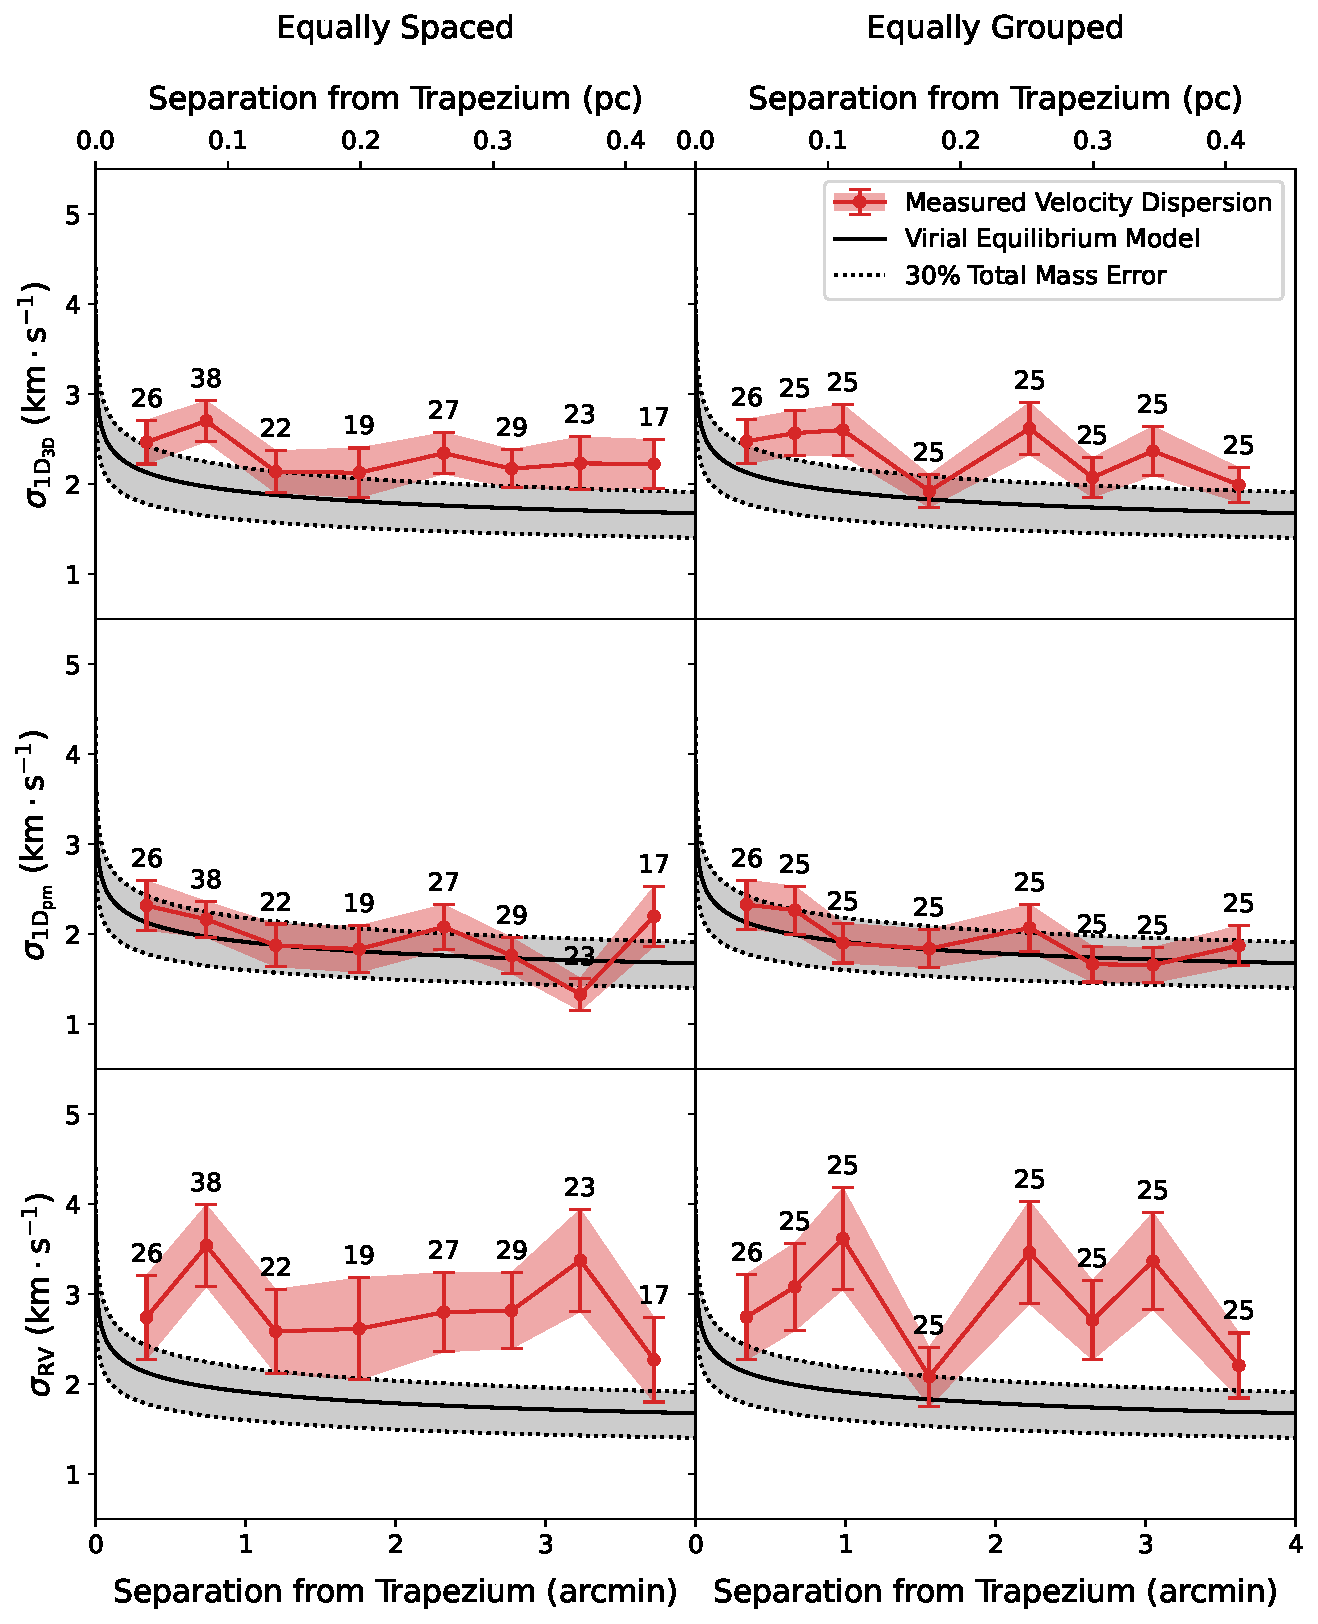
\includegraphics[width=0.8\linewidth]{figures/chapter1/vdisp_vs_sep.pdf}
    \caption[Velocity dispersion vs. separation of the ONC]{Velocity dispersion as a function of separation from the cluster center. The observed velocity dispersion is shown in red, whereas the requirement of viral equilibrium is illustrated as the black line. The dotted line and the shaded area indicate a $30\%$ total mass error on the virial equilibrium model. The sources are binned equally spaced in the left column, i.e., with identical bin width, and equally grouped in the right column, i.e., with an almost identical number of sources in each bin. The number of sources is labeled on top of each bin. \textit{Top:} 1D velocity dispersion in all directions; \textit{Middle:} 1D velocity dispersion of the proper motions; \textit{Bottom:} Velocity dispersion of the radial velocities.}
    \label{fig:vdisp}
\end{figure}

Another dynamical state we can infer from the velocity dispersion is whether energy equipartition has occurred in the cluster. The velocity dispersion should be inversely proportional to the square root of the stellar mass in a cluster where energy equipartition has already occurred via gravitational interactions. Previously, \citet{Hillenbrand-1998} did not see evidence of equipartition in the ONC. Here we re-evaluate this conclusion with our newest data. Figure~\ref{fig:vdisp vs mass} shows the equally grouped 1D velocity dispersion of all three directions $\sigma_\mathrm{1D_{3D}}$, 1D velocity dispersion in the proper motion directions $\sigma_\mathrm{1D_{pm}} = \sqrt{\left(\sigma_\mathrm{RA}^2 + \sigma_\mathrm{DEC}^2\right)/2}$, and radial direction as a function of the stellar mass. The $-1/2$ slope is clearly not present. This is conceivable as the relaxation time of the cluster is estimated to be $6.5$~Myr \citep[][]{Hillenbrand-1998}, much larger than the age of the cluster of about $2$~Myr. Therefore, energy equipartition has not yet taken place in the central ONC, in agreement with \citet{Hillenbrand-1998}. 



\subsection{Velocity-Mass Relation}
\label{onc-subsec:v-m}

\begin{figure*}[htb!]
    \centering
    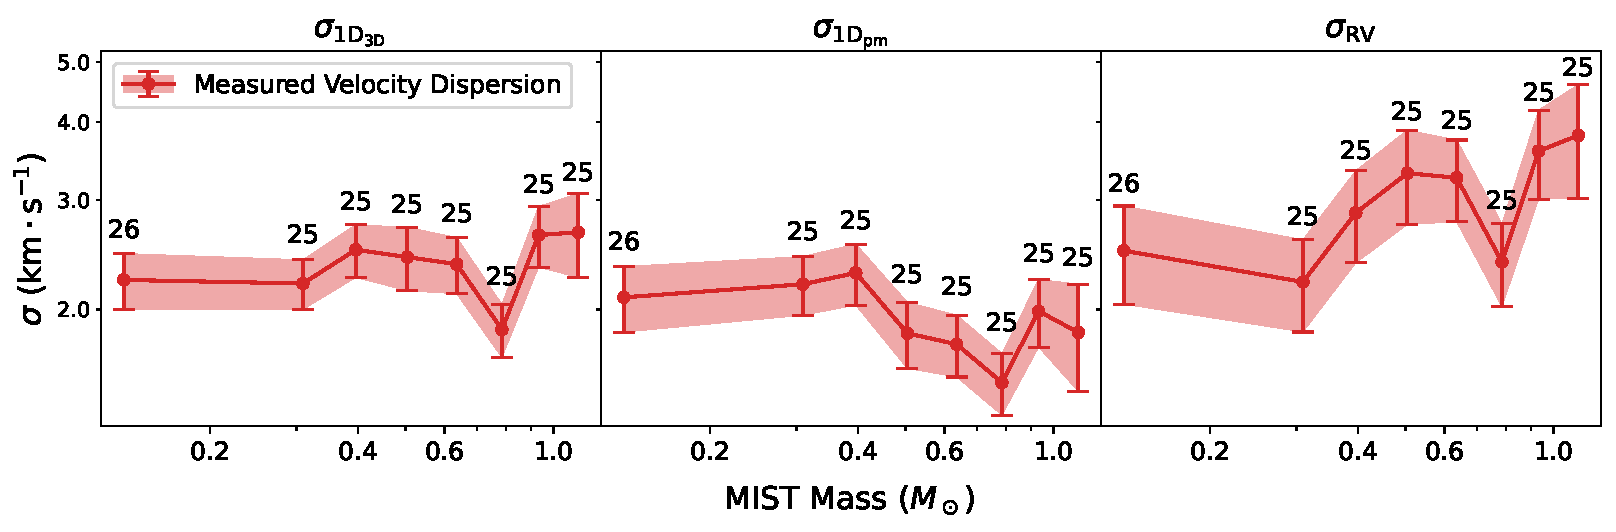
\includegraphics[width=\linewidth]{figures/chapter1/vdisp_vs_mass.pdf}
    \caption[Velocity dispersion vs. stellar mass]{Velocity dispersion as a function of stellar mass interpolated from the MIST model. From left to right, the three subfigures show the 1D velocity dispersion of all three directions $\sigma_\mathrm{1D_{3D}}$, the 1D velocity dispersion of the proper motions $\sigma_\mathrm{1D_{pm}}$, and the radial velocity dispersion $\sigma_\mathrm{1D_{RV}}$, respectively. The sources are grouped with equal sizes, and the number of sources in each bin is labeled on top of the corresponding bin.}
    \label{fig:vdisp vs mass}
\end{figure*}

\begin{figure*}[htb!]
    \centering
    \gridline{\fig{figures/chapter1/MIST-linear-0.10pc.pdf}{0.496\linewidth}{(a)}
              \fig{figures/chapter1/BHAC15-linear-0.10pc.pdf}{0.496\linewidth}{(b)}}
    \gridline{\fig{figures/chapter1/Feiden-linear-0.10pc.pdf}{0.496\linewidth}{(c)}
              \fig{figures/chapter1/Palla-linear-0.10pc.pdf}{0.496\linewidth}{(d)}}
    \caption[Relative velocity vs. stellar mass]{The computed velocity relative to the center of mass of the neighbors of each source within a $0.1$-pc (or $53\arcsec$) radius versus stellar mass. Four models are used to interpolate the stellar mass: (a) MIST model; (b) BHAC15 model; (c) Feiden model; (d) Palla model. In each subfigure, the data are represented as blue points and error bars. The value of the kernel density estimator (KDE) is colored in blue in the background to show the distribution of the data. The purple line marks the $84$-th percentile of the KDE value. The equally-grouped running average, along with its uncertainties, is marked and filled in red. The black line shows the best linear fit to the data, with the slope $k$ and intercept $b$ labeled in the legend. $p$-value and Pearson's correlation coefficient $R$ are labeled in the bottom right of each figure. All four models display both a negative slope of the linear fit and a negative correlation coefficient.}
    \label{fig:vrel-mass}
\end{figure*}


With kinematic information and mass estimates for sources in the central ONC, we can look for correlations between masses and velocities, which is indicative of whether stars form via filament fragmentation. Figure~\ref{fig:vrel-mass} shows the velocity of each source relative to its neighbors (including itself) within a $0.1$~pc (or $53\arcsec$) radius versus their masses derived from the four different evolutionary models described in Section~\ref{onc-subsec:mass}. The radius within which sources are considered as neighbors can be varied and will be further discussed in Section~\ref{onc-subsec:teff offset}. The median number of neighbors for each source is $11$. The data are shown in blue. We employ the Gaussian kernel density estimation (KDE) to visualize the distribution of the data, and the value of the estimator is colored in blue in the background. The $84$-th percentile of the estimator value is marked as the purple curve. As can be seen, the envelope displays a negative trend on its upper edge. To look at this trend more globally, we show the equally grouped running average in red.  Since the trend of velocity versus mass appears roughly linear, we fit a linear relationship $v_\mathrm{rel}=k*m+b$ to the data using the \texttt{scipy.stats.linregress} function \citep[][]{scipy}, where $v_\mathrm{rel}$ is the relative velocity, $m$ is the stellar mass, $k$ and $b$ are the slope and intercept, respectively.  To determine the best-fit slope and intercept and their associated uncertainties, we resample the relative velocity and the mass of each source from a normal distribution centered at the observed values, with standard deviations being the uncertainty of measurement. Only positive values are kept for the linear fitting. We resampled $10^5$ times and each time conducted a linear regression on the data. The median of the recorded slope and intercept is chosen as the best fit values, while half the differences between the $16$ and $84$-th percentiles are considered as their associated uncertainties. The values and uncertainties of the slope $k$ and the intercept $b$ are labeled in the legend in each figure. We utilize the measured values to calculate the $p$-value for the linear fit, with the null hypothesis being that the slope is zero. As all of the $p$-values are less than $0.05$, we can safely reject the null hypothesis and conclude that the negative correlation is statistically significant. Apart from the linear fit, we also calculate the Pearson correlation coefficient $R$ as a reflection of the degree of their correlation.  The best-fit value and uncertainty of $R$ are determined by resampling in the same way as the linear fit.  As can be seen from the figure, all four models display a negative correlation. 

\begin{figure}[htb!]
    \centering
    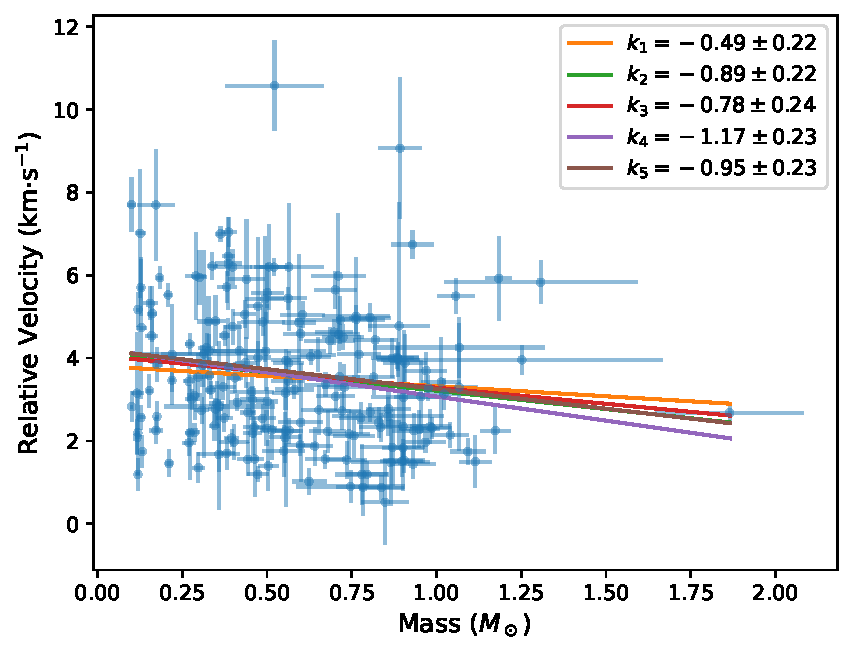
\includegraphics[width=0.7\linewidth]{figures/chapter1/KFold.pdf}
    \caption[Cross validation of negative correlation between relative velocity and stellar mass]{$5$-fold cross-validation of the negative correlation between relative velocity and stellar mass. The slope and its associated uncertainty for each linear regression $k_1$--$k_5$ is labeled in the legend. This test adopted the stellar masses derived from the MIST model.}
    \label{fig:kfold}
\end{figure}

We utilized $5$-fold cross-validation to verify the statistical significance of the negative correlation between relative velocity and stellar mass and ensure that it is not driven by only a few outlier datapoints. The data is randomly partitioned into $5$ equally sized groups, commonly referred to as `folds'. Linear regression is then performed on $4$ groups of the data, leaving out a different group each time. The slope of the resulting $5$ linear regressions in the case of the MIST model is shown in Figure~\ref{fig:kfold}. The uncertainty-weighted average of the slope across the $5$ folds is $-0.85$, and the standard deviation is $0.22$, consistent with the result shown in Figure~\ref{fig:vrel-mass} (a). Therefore, by randomly selecting $5$ different sets of $80\%$ of the data but still arriving at the same conclusion, we further validated our finding that the relative velocity is negatively correlated with stellar mass.

\subsection{Effective Temperature Offset Between NIRSPAO and APOGEE}
\label{onc-subsec:teff offset}
\begin{figure}[htb!]
    \centering
    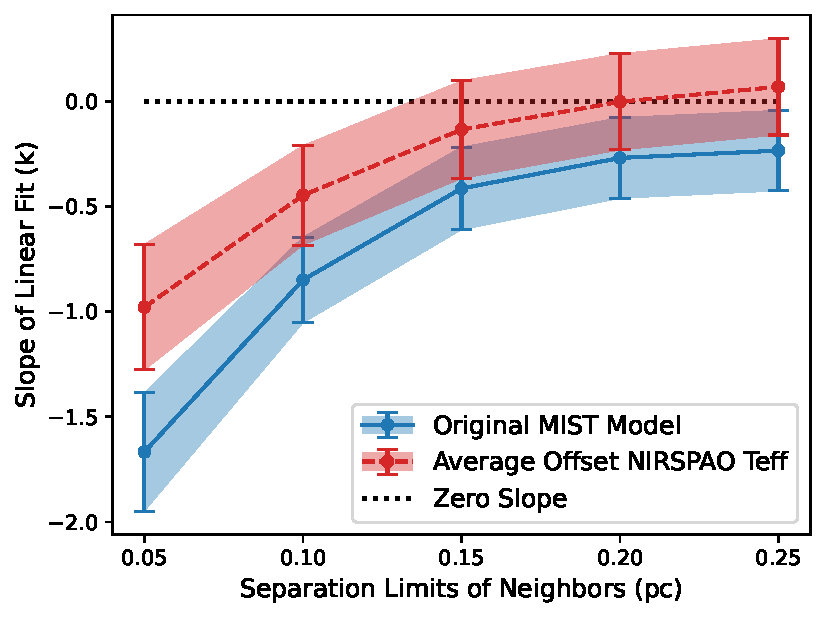
\includegraphics[width=0.7\linewidth]{figures/chapter1/slope_vs_sep.pdf}
    \caption[Slope of linear fit vs. separation limit of neighbors]{Slope of linear fit as a function of separation limit of neighbors. We selected $0.1$~pc when analyzing the velocity-mass relation in Section~\ref{onc-subsec:v-m}. Here, the separation limit within which sources are counted as neighbors is varied to explore how the linear slope changes. The blue line shows the stellar mass under the MIST model with the derived $T_\mathrm{eff}$, while the red line shows the MIST stellar mass after offsetting the NIRSPAO $T_\mathrm{eff}$ by the average difference of $526.25$~K between NIRSPAO and APOGEE. The dashed line shows the zero-slope, or no correlation. The negative correlation between relative velocity and mass is more evident locally within a smaller radius when calculating the relative velocity.}
    \label{fig:slope_vs_mass}
\end{figure}

Despite using the same spectral modeling algorithm, there seems to be a systematic discrepancy in the effective temperatures between the $17$ cross-matched NIRSPAO and APOGEE sources in our sample. Figure~\ref{fig:slope_vs_mass} shows the comparison. Effective temperatures derived from APOGEE spectra are higher than NIRSPAO results, with a weighted average offset of $586$~K and a maximum difference of $892$~K. Several reasons may cause this difference. First, the spectra of APOGEE and NIRSPEC are in $H$ and $K$ bands, respectively. The spectral features that determine the modeled stellar parameters are therefore different between the two sets of observations. For example, the CO lines are more sensitive to low-temperature sources, as the intended objective of the NIRSPAO observation is to observe low-mass stars. Additionally, considering the highly embedded and crowded nature of the region, extinction and reddening are not identical in $H$ and $K$ bands. A future study will simulate the effect of reddening on temperature estimates. Additionally, to enhance the quality of modeling, especially RV, there is an ongoing effort to model the fringing in the spectrum, which is the primary contributor to the residuals.  For the purpose of this study, NIRSPAO estimated effective temperatures are prioritized over APOGEE results.

To evaluate the impact of choosing the NIRSPAO temperatures for mass estimates, we offset the NIRSPAO temperature by the weighted-averaged difference of $586$~K to simulate the effect on the velocity-mass relation discussed in Section~\ref{onc-subsec:v-m}. Figure~\ref{fig:slope_vs_mass} shows the slope of the linear fit before and after the offset as a function of the radius within which sources are considered as neighbors when calculating relative velocities. It can be seen that the negative correlation with mass is weaker but still exists after inflating the NIRSPAO temperature to match the APOGEE values. Either before or after the offset, the negative trend between relative velocity and mass is more evident locally, i.e., a smaller threshold of radius for sources to be considered as neighbors. Discretion is advised for the near-zero slope at larger neighboring radius, as the entire area being analyzed is about $0.45$~pc in radius. More sources on the periphery would have incomplete neighbors, which could affect the accuracy of the correlation and the underlying significance.


\subsection{Preferred Proper Motion Direction}
\label{onc-subsec:pm}

\begin{figure}[htb!]
    \centering
    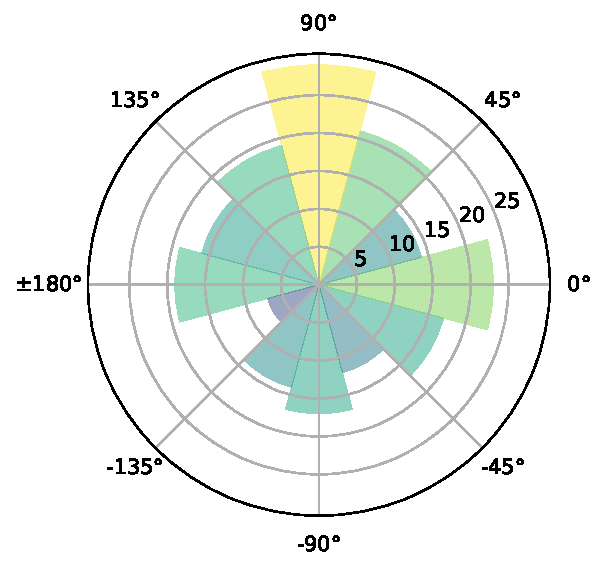
\includegraphics[width=0.7\linewidth]{figures/chapter1/pm_direction.pdf}
    \caption[Distribution of proper motion directions]{Distribution of the angle between the displacement vector from the center of the ONC and the proper motion vector on the plane of the sky. Positive values stand for clockwise rotation about the center of the ONC, and vice versa. $0^\circ$ stands for expansion and $\pm180^\circ$ means contraction towards the center. More sources are in the $0^\circ$ than $\pm180^\circ$ bin agrees with the finding that the ONC is experiencing a slight expansion \citep[][]{Kounkel-2022}. The peak at $90^\circ$ here illustrates that the sources have a preference for clockwise rotation on the plane of the sky around the ONC center.}
    \label{fig:pm direction}
\end{figure}

Previous studies identified signs of expansion within the ONC \citep[e.g.,][]{Kounkel-2022}, and a rotational preference in the proper motions \citepalias{Theissen-2022}. With a combination of HST and Gaia measurements, we are able to re-evaluate the above findings in greater detail. A polar histogram of the angle between the stellar proper motion vector and the separation vector from the ONC center is shown in Figure~\ref{fig:pm direction}. Specifically, a positive angle represents clockwise rotation about the ONC center, whereas a negative angle represents counter-clockwise rotation. An angle of zero indicates the source is moving radially outward with respect to the ONC center on the plane of the sky, while $-180^\circ$ means the source is moving towards the center. More sources are in the $0^\circ$ than $\pm180^\circ$ bin agrees with the finding that the ONC is experiencing a slight expansion \citep[][]{Kounkel-2022}. The peak around $90^\circ$ in Figure~\ref{fig:pm direction} illustrates that the center of the cluster is undergoing a clockwise rotation. This is consistent with the finding in \citet{Strand-1958}. \citetalias{Theissen-2022} identifies a rotational preference in both $+90^\circ$ and $-90^\circ$, or clockwise and counter-clockwise directions simultaneously. The increase in sample size shows that the ONC core is actually experiencing a clockwise rotation, though a larger sample size would help confirm this trend.


\section{Binary Candidates and Binary Simulation}
\label{onc-sec:binary}
Among the $23$ sources that have multiple epochs of RV measurements, $4$ of them exhibited strong variability in their radial velocities. We therefore report the discovery of two candidate binary systems, Paranego 1837, Brun 590, V* V1337 Ori, and V* V1279 Ori.

\subsection{Parenago 1837}
\label{onc-subsec:parenago}
\begin{figure}[htb!]
    \centering
    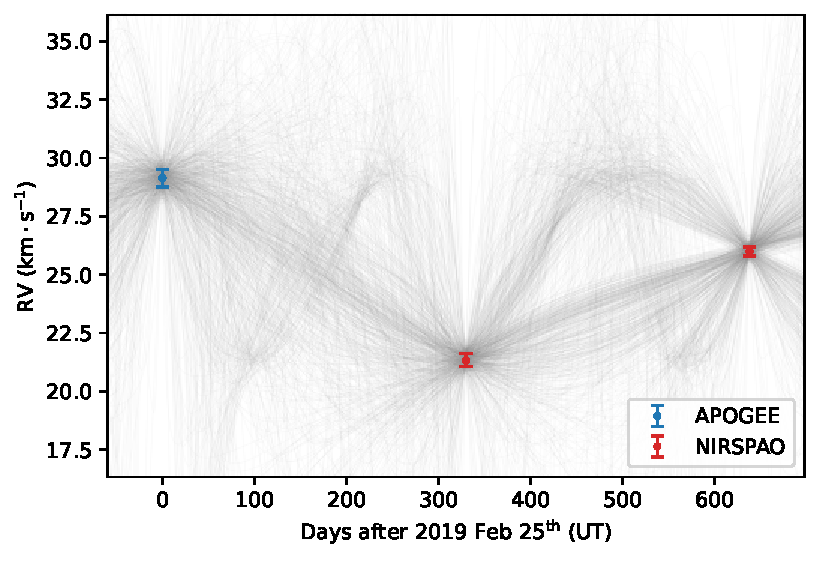
\includegraphics[width=0.7\linewidth]{figures/chapter1/Parenago1837-Orbital_Fits.pdf}
    \caption[Parenago 1837 orbital fit]{The RVs after barycentric correction of the identified binary candidate Parenago 1837 measured by APOGEE and NIRSPAO in three epochs. $876$ potential orbital fits with a period between $\Delta t/3$ ($213$~days) and $2\Delta t$ ($1276$~days) are shown in gray. Three different modes of orbits can be clearly seen from the figure, corresponding to periods within ranges of $\Delta t/4\sim\Delta t/2$, $\Delta t/2\sim\Delta t$, and $\Delta t\sim2\Delta t$, respectively.}
    \label{fig:orbital fits}
\end{figure}

\begin{figure}[htb!]
    \centering
    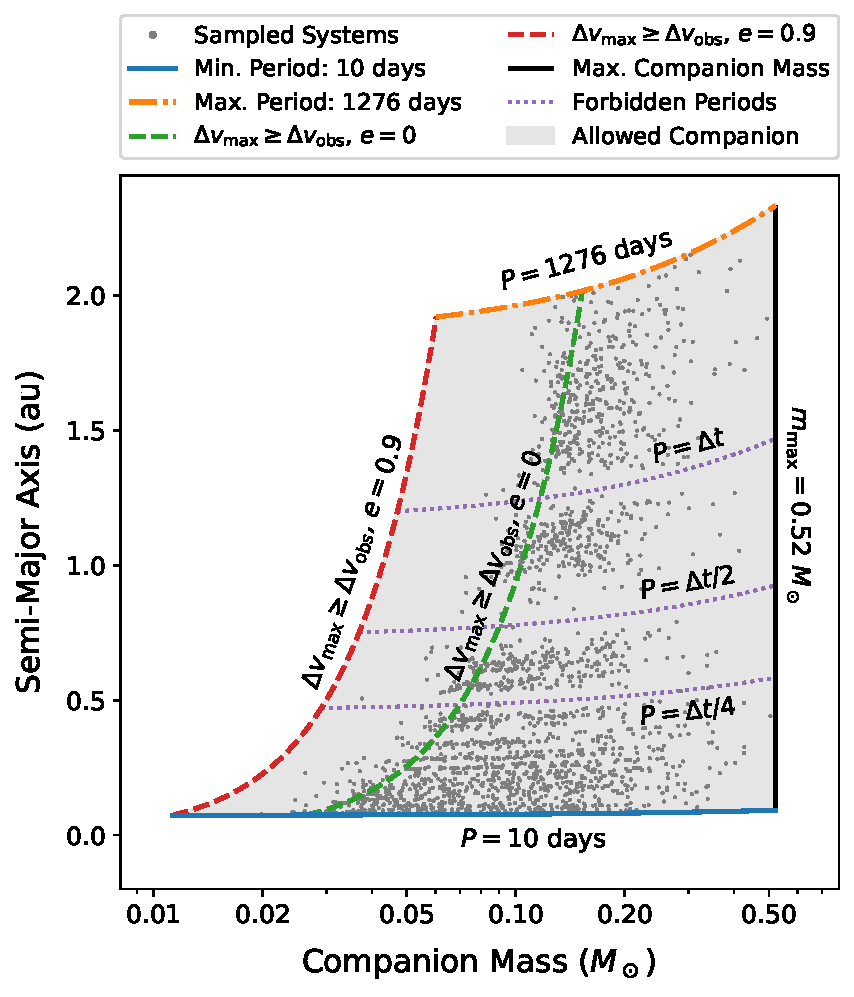
\includegraphics[width=0.7\linewidth]{figures/chapter1/Parenago1837-Allowed_Param.pdf}
    \caption[Orbital parameter space constraint of the companion of Parenago 1837]{Allowed companion in the semi-major axis-companion mass parameter space and $2126$ sampled systems from \textit{The Joker}. Each sampled system is shown as a small gray point. The period range between $10$~days and twice the observation time span $2\Delta t$ or $1276$~days is indicated by the blue solid line at the bottom and the amber dash-dotted line at the top, respectively. The left boundary is set by the required variation in orbital velocity, which is illustrated in green dashed line for circular orbits, and in red for orbits with eccentricity up to $0.9$ (see Equation~\ref{eq:deltav}). Assuming a companion smaller than the observed primary mass of $0.52~M_\odot$ sets the limit shown by the dotted black line to the right. The shaded area is the allowed parameter space within which the companion can reside with the assumptions above. The forbidden periods, which are an integer fraction of the observation time span $\Delta t$, are labeled as the purple dotted line.}
    \label{fig:allowed param}
\end{figure}

Parenago 1837, or HC2000 546, exhibits variation in its RVs measured in three different epochs, first by APOGEE, followed by two observations by NIRSPAO. According to \textit{Gaia} DR3, it has a G magnitude of $13.54$, with BP (blue pass) magnitude of $13.23$ and RP (red pass) magnitude of $11.95$. The derived stellar mass of the primary is $0.52\pm0.04~M_\odot$ according to the MIST model, assuming the primary light dominates the observed spectra. The RVs after barycentric correction are $29.14\pm0.38\mathrm{km}\,\mathrm{s^{-1}}$, $21.34\pm0.28~\mathrm{km}\,\mathrm{s^{-1}}$, and $25.99\pm0.19~\mathrm{km}\,\mathrm{s^{-1}}$ measured on on 2019 February 25$^\mathrm{th}$ (UT), 2020 Janurary 21$^\mathrm{st}$ (UT), and 2021 October 20$^\mathrm{th}$ (UT), respectively. The total time span between the first and last observation $\Delta t=638$ days. Figure~\ref{fig:orbital fits} shows each measured RV at the time of observation. The blue and red error bars indicate the results from APOGEE and NIRSPAO, respectively.

To explore the possible properties of the companion, we sample the possible orbital parameters of the system using a Monte Carlo rejection sampler, \textit{The Joker} \citep{thejoker}. \textit{The Joker} requires specifying the priors, including the period limits, the RV semi-amplitude $K$, and the standard deviations of the velocity trend priors. We limit the periods to between $10$ days and twice the observation time span $\Delta t$, or $1276$ days. Orbital solutions with arbitrarily long periods and large RV variations can be obtained with only $3$ epochs of observations. Therefore, an upper limit on the period is a reasonable assumption considering the low mass of the object. The semi-amplitude prior is set to $5~\mathrm{km}\,\mathrm{s}^{-1}$, slightly larger than the variation of the RVs. The standard deviations of the velocity priors are set to be a relatively large value of $100~\mathrm{km}\,\mathrm{s}^{-1}$ to allow the sampler to fully explore the orbital parameter space. Additionally, we replace the default prior distribution of eccentricity with a uniform distribution between $0$ and $0.9$ to evenly explore the parameter space. We generate $10^5$ prior samples and $2126$ orbital solutions that match the observed RVs remain after the rejection sampling. The semi-amplitude of the primary's RV variation $K$ is related to stellar masses as
\begin{equation}
\label{eq:K_original}
    K=\frac{m}{M+m}\frac{2\pi a\sin I}{T\sqrt{1-e^2}}~,
\end{equation}
where $M$ is the primary mass, $m$ is companion mass, $T$ is the orbital period, $a$ is the semi-major axis, $I$ is the inclination, and $e$ is the eccentricity of the orbit \citep{Murray-2010}. The semi-major axis $a$ can be expressed as the stellar masses and the orbital period $T$ according to Kepler's third law
\begin{equation}
\label{eq:a}
    a=\left(\frac{\mu}{4\pi^2}T^2\right)^{1/3}~,
\end{equation}
where $\mu=G\left(M+m\right)$ is the standard gravitational parameter. Substituting Equation~\ref{eq:a} into Equation~\ref{eq:K_original}, $K$ can be expressed as a function of stellar masses, eccentricity, and orbital period
\begin{equation}
\label{eq:K}
    K=\frac{m}{M+m}\frac{2\pi\sin I}{\sqrt{1-e^2}}\left(\frac{\mu}{4\pi^2T}\right)^{1/3}~.
\end{equation}
Therefore, we can solve for the minimum companion mass when $I=\pi/2$ given the $K$, $T$, and $e$ for each sampled system from Equation~\ref{eq:K} with the derived primary mass of $0.50~M_\odot$. Figure~\ref{fig:allowed param} shows the distribution of sampled systems and the theoretically allowed region in the semi-major axis-companion mass parameter space. The bottom and top limits are set by the assumed period range between $10$ days and $1276$ days. The left boundary is set by the constraint that the maximum variation in orbital velocity difference when the orbit is observed from an edge-on direction must exceed the observed amplitude of RV change, i.e., 
\begin{equation}
\label{eq:deltav}
\begin{split}
\Delta v_\mathrm{max}   & = v_p + v_a \\
                        & = \frac{m}{M+m}\sqrt{\frac{\mu}{a}}\left(\sqrt{\frac{1+e}{1-e}} + \sqrt{\frac{1-e}{1+e}}\right) \\
                        & = 2\frac{m}{M+m}\sqrt{\frac{\mu}{a\left(1-e^2\right)}} \\
                        & \geq\Delta v_\mathrm{obs}~,
\end{split}
\end{equation}
where $v_\mathrm{max}$ is the maximum orbital velocity difference, $\Delta v_\mathrm{obs}$ is the observed RV difference, and $v_p$, $v_a$ denotes the orbital velocity at perihelion and aphelion, respectively \citep{Murray-1999}. Both the cases when $e=0$ and $e=0.9$ are plotted in Figure~\ref{fig:allowed param} in green and red dashed lines. As can be seen, most sampled systems are within the green line, with a small fraction residing between the green and the red line. Assuming a companion smaller than the observed primary mass of $0.50~M_\odot$ sets the limit shown by the dotted black line to the right. The gaps visible in the sampled systems and marked by purple dotted lines are the forbidden periods of integer number fractions of the observation time span $\Delta t$, as the first and last measured RVs are not identical.

$876$ potential orbital fits with a period greater than $\Delta t/3$ or $213$ days but less than $2\Delta t$ or $1276$ days are plotted in gray in Figure~\ref{fig:orbital fits}. Three different modes of orbits can be clearly seen from the figure, corresponding to periods within ranges of $\Delta t/4\sim\Delta t/2$, $\Delta t/2\sim\Delta t$, and $\Delta t\sim2\Delta t$, respectively.

Despite the limited epochs of observation, we are able to infer the approximate mass and separation of the companion thanks to the derived primary mass under reasonable assumptions on the orbital period between $10$ days and twice the observation time span of $1276$ days. Parenago 1837 is a candidate binary system consisting of a primary of $0.52\pm0.04~M_\odot$ and most likely a companion of $\sim0.03$--$0.3~M_\odot$, with a separation of less than $2$~au. Further observation is needed to more robustly constrain its orbit.


\subsection{V* V1337 Ori}
\label{onc-subsec:V1337}
V* V1337 Ori, or HC2000 214, is another binary candidate. The original APOGEE results have $6$ visits on the object. The difference in RV is as large as $17.87~\mathrm{km}\,\mathrm{s}^{-1}$ throughout all the visits, which makes it very likely to be a binary system. However, currently we only have one reanalyzed APOGEE result. Single-epoch reanalysis is required to further constrain its orbit. For consistency, we utilize the reanalyzed APOGEE result of $45.52\pm1.25~\mathrm{km}\,\mathrm{s}^{-1}$, followed by NIRSPAO measurement on 2020 January 20$^\mathrm{th}$ (UT) of $36.93\pm1.05~\mathrm{km}\,\mathrm{s}^{-1}$. The two measurements differ by more than $7$-sigma. The inferred primary mass is $0.52\pm0.14~M_\odot$. Due to the limited measurements, it would be challenging to do a similar analysis of Parenago 1837. Therefore, reanalysis on individual previous APOGEE visits or future observations is needed to confirm and constrain this binary system.


\subsection{V* V1279 Ori}
V* V1279 Ori, or HC2000 170, is a source of $0.40\pm0.03~M_\odot$ according to the MIST model. It has a RV measurement of $23.7\pm1.0~\mathrm{km}\,\mathrm{s}^{-1}$ in the RV survey by \citet{Tobin-2009}. Our Keck NIRSPAO measures a RV of $32.70\pm1.62~\mathrm{km}\,\mathrm{s}^{-1}$ on 2022 Jan 18$^\mathrm{th}$ (UT), more than $5$--$\sigma$ different from each other.


\subsection{Brun 590}
Brun 590, or HC2000 172, is another candidate of $0.60\pm0.06~M_\odot$ according to the MIST model with $2$ RV measurements. 
NIRSPAO measures $23.36\pm0.29~\mathrm{km}\,\mathrm{s}^{-1}$ on 2022 Jan 20$^\mathrm{th}$ (UT). Different interpretations of APOGEE RV is present in the literature. The reanalyzed APOGEE RV from \citetalias{Theissen-2022} is $29.26\pm1.23~\mathrm{km}\,\mathrm{s}^{-1}$, while \citet{Kounkel-2019} gives $19.320\pm1.182~\mathrm{km}\,\mathrm{s}^{-1}$ after removing the systematic effect of temperature and epoch-dependent offsets \citep[][]{Cottaar-2014}. Additional validation and observation is required to confirm whether it is a binary system and constrain the orbit.

\subsection{Binary Simulation}
\label{onc-subsec:binary simulation}

\subsubsection{Velocity Dispersion}
\begin{figure}[htb!]
    \centering
    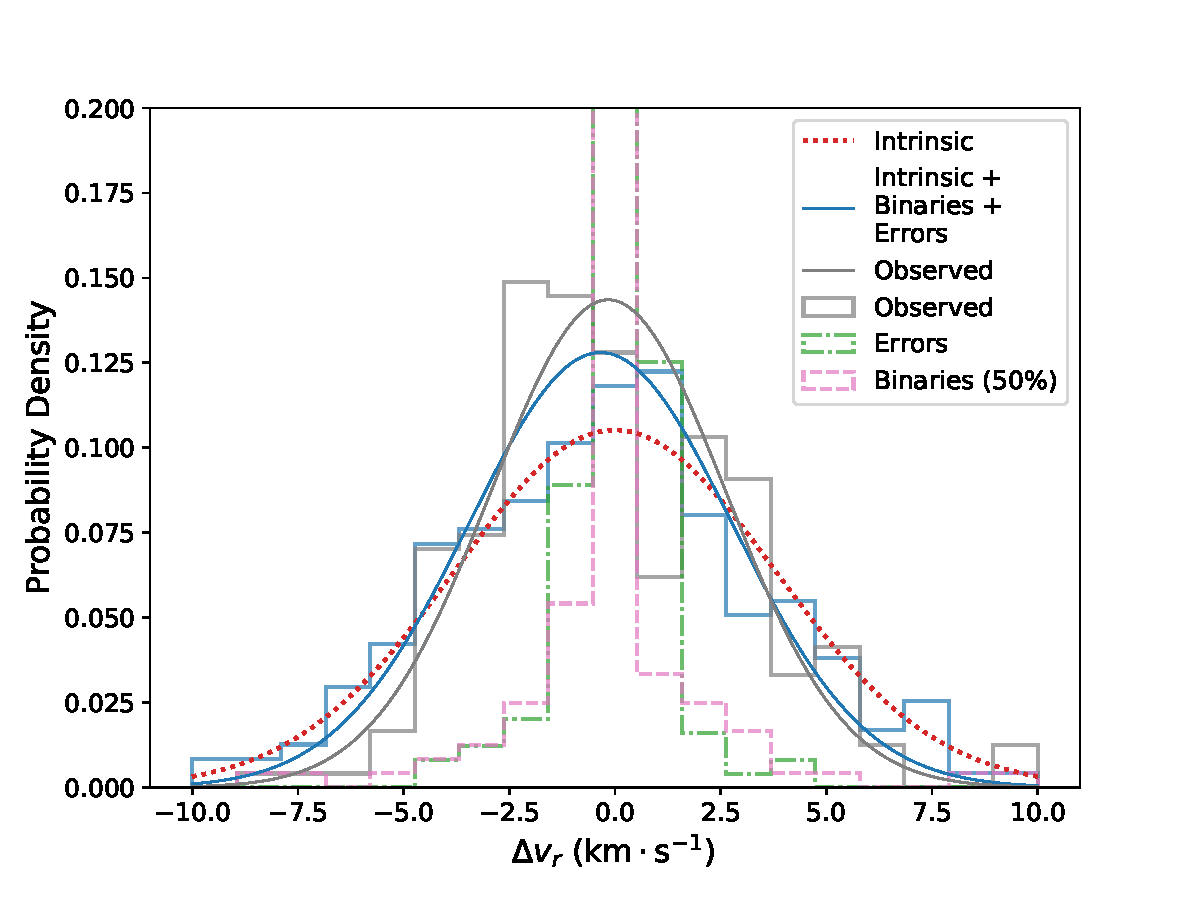
\includegraphics[width=\linewidth]{figures/chapter1/Binary_Simulation_Histogram.pdf}
    \caption[Radial velocity dispersion distribution of binary simulation]{Radial velocity dispersion in a simulation with binary fraction set to $50\%$. The red dotted line shows the intrinsic velocity dispersion. The gray histogram and curve show the observed distribution and fitted normal distribution. The synthetic velocity dispersion with contributions from the intrinsic velocity dispersion, the measurement errors, and the binary offset is shown in blue. The dash-dotted green histogram shows the measurement errors, and the pink dashed histogram shows the contribution from the binaries.}
    \label{fig:binary histogram}
\end{figure}

\begin{figure}[htb!]
    \centering
    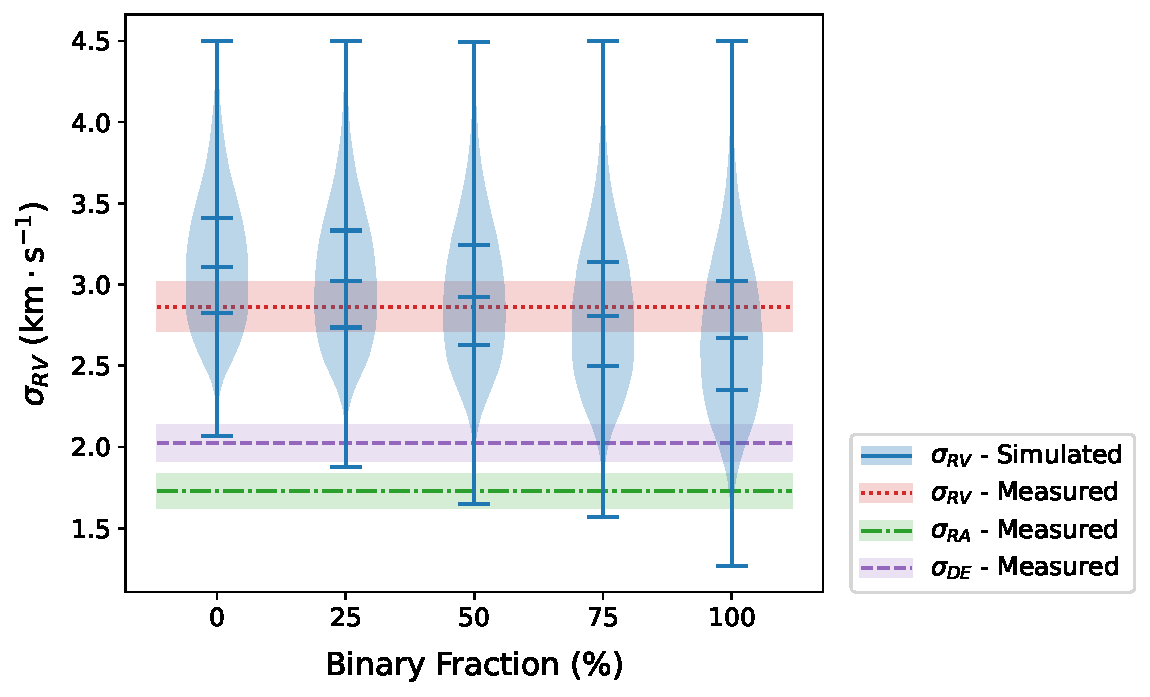
\includegraphics[width=\linewidth]{figures/chapter1/Binary_Simulation_Violin.pdf}
    \caption[Violin plot of the intrinsic radial velocity dispersion in binary simulation]{Binary simulation result of the intrinsic radial velocity dispersion. The blue violin plot shows the distribution of the $10^5$ simulated synthesized radial velocity dispersion under different imposed binary fractions, with the $0$-th, $16$-th, $50$-th, $84$-th, and $100$-th percentiles marked by the horizontal bars. The measured velocity dispersion in radial, right ascension, and declination directions is shown in red dotted line, green dash-dotted line, and purple dashed lines, respectively.}
    \label{fig:binary violin}
\end{figure}

The Keck can spatially resolve binaries with separations larger than $25$~mas, or about $10$~au at the distance of the ONC \citep{Lacour-2011}. Closer binary systems can not be resolved. Currently, we do not have a measurement of the close binary fraction in the ONC, as most of the published work has focused on visual binaries.  A large fraction of optically unresolved binaries will have a profound effect on the IVD. Therefore, we use the \texttt{velbin} package \citep[][]{Cottaar-2014, Foster-2015} to simulate the effects of unresolved binaries on our IVD measurements following a similar procedure as described in \citet{DaRio-2017}, \citet{Karnath-2019}, and \citetalias{Theissen-2022}. $235$ systems are generated across the binary fraction range from $0$ to $1$ with a step size of $0.25$, as is the total number of NIRSPEC and APOGEE sources used to generate the IVD.

The synthetic simulated RV distribution consists of three components: the systematics, the measurement uncertainty, and the binary offset. We briefly describe the steps to reproduce the three components below. First, a random intrinsic velocity dispersion is drawn from a uniform distribution between $1$ and $4.5~\mathrm{km}\,\mathrm{s}^{-1}$, which roughly covers a symmetric range on both ends lower and higher than the measured radial velocity dispersion of $2.87\pm0.15~\mathrm{km}\,\mathrm{s}^{-1}$. The systematics are the product of the intrinsic velocity dispersion and a standard normal distribution of length $235$. The simulated measurement uncertainty is generated by randomly sampling from the cumulative distribution function (CDF) constructed from the observed measurement error distribution, and multiplied by another standard normal distribution. Similarly, a mass distribution is generated by sampling from the CDF constructed by the interpolated mass distribution of the $235$ sources. An ensemble of stellar binary systems with uniform distribution of mass ratio and eccentricities is then simulated using this mass distribution with \texttt{velbin}, which in turn gives the radial velocity offset given the binary fraction.

The above process is repeated, and the first $10^5$ simulations are kept in which the standard deviation of the synthetic distribution lies within $2\sigma$ from the standard deviation of the observed distribution, where $\sigma$ is the uncertainty in the velocity dispersion in the radial component, or $0.15~\mathrm{km}\,\mathrm{s}^{-1}$ in our case. Note that radial velocity offsets with an absolute value greater than $7~\mathrm{km}\,\mathrm{s}^{-1}$ are truncated when fitting for the standard deviations to avoid the impact of extreme values.

Figure~\ref{fig:binary histogram} shows the simulated and observed velocity distributions in one of the simulations with binary fraction set to $50\%$. Figure~\ref{fig:binary violin} shows the distribution of the $10^5$ simulated IVDs that satisfy the aforementioned criterion under different imposed binary fractions. The blue violin plot illustrates the distribution of the simulated radial velocity dispersion. For comparison, IVDs in the radial, right ascension, and declination directions are shown in red dotted lines, green dash-dotted lines, and purple dashed lines, respectively. The crossing point between the measured radial velocity dispersion and the interpolation of the median of the simulated radial velocity dispersion at each binary fraction is at $62.54\%$. In other words, a binary fraction $\gtrsim~62.54\%$ is required to account for our measured higher velocity dispersion in the radial direction if the higher value is solely induced by binaries, which is unreasonably high compared to estimates in the literature. As can be seen from Figure~\ref{fig:binary violin}, the IVD of the radial component is higher than the other two directions, regardless of the simulated binary fraction. Therefore, the binarity alone is not sufficient to explain the larger values in the radial component. 


\subsubsection{Unresolved Binary Mass}
Unresolved close binaries are a potential source of systematic effects that could influence our results. Despite a lack of measurement of spectroscopic binaries in the region, we utilized multiplicity surveys collected in \citet{Offner-2023} and conducted a quantitative test on how the unresolved close binaries affect the correlation between relative velocity and stellar mass. Since Keck has a spatial resolution of $10$~au at the distance of the ONC, we adopted the close binary fraction (CBF) within $10$~au for brown dwarfs and main sequence stars to calculate the mass contribution from unresolved binaries. Historically, the distribution of the mass ratio $q$ is approximated by a power-law $f_q\propto q^\gamma$. We chose the values of $\gamma$ for binaries with a separation between $1$~au and $10$~au. The expectation of the mass of the hidden companion is therefore
\begin{equation}
    \mathrm{CBF}\times M\times\frac{\int_0^1 q\cdot f_q dq}{\int_0^1 f_q dq}~,
    \label{eq:binary mass}
\end{equation}
where the values of CBF and $q$ is determined by the observed primary mass according to \citet{Offner-2023}. Specifically, we utilized the values from the surveys in \citet{Winters-2019, Raghavan-2010}, and \citet{Tokovinin-2014} in order of increasing stellar mass. Note that $\gamma$ is assumed to be $0$ where the value is unavailable. The closest available values are utilized for sources situated in gaps of stellar mass ranges. For overlapping mass ranges, we adopt the values in the survey where the source is closer to the center of its mass range. Consequently, the adopted values are
\begin{equation}
\begin{aligned}
    &\mathrm{CBF}=16\%,&\gamma=0\quad&\mathrm{if}\quad0.075<M<0.15~,\\
    &\mathrm{CBF}=14\%,&\gamma=0.7\quad&\mathrm{if}\quad0.15<M<0.3~,\\
    &\mathrm{CBF}=15\%,&\gamma=0.1\quad&\mathrm{if}\quad0.3<M<0.675~,\\
    &\mathrm{CBF}=20\%,&\gamma=0.2\quad&\mathrm{if}\quad0.675<M<1.0875~,\\
    &\mathrm{CBF}=14\%,&\gamma=0.4\quad&\mathrm{if}\quad1.0875<M<1.5~.
\end{aligned}
\end{equation}
Substituting the above values back into Equation~\ref{eq:binary mass} for each source gives the expectation of the mass of the unresolved close binary.  As a result, the stellar mass increases by $8$--$14\%$.  Additionally, the negative correlation in Figure~\ref{fig:vrel-mass} persists after accounting for this excess in mass. The unresolved binaries only produce a marginally flatter linear fit, but still with a negative slope. For a quantitative comparison, the slopes in Figure~\ref{fig:vrel-mass} becomes $-0.75\pm0.18$, $-1.05\pm0.19$, $-0.71\pm0.19$, and $-0.72\pm0.14$ for MIST, BHAC15, Feiden, and Palla models respectively.  This is because the stellar mass on the higher-mass end is shifted further right in Figure~\ref{fig:vrel-mass}, while the change in mass of the lower-mass source is limited.  Therefore, the excess mass stretches the distribution of the data points horizontally, but the negative correlation persists.


\section{Discussion}
\label{onc-sec:discussion}

\subsection{Kinematic Structure of the ONC and Star Formation Implications}

In this analysis, we have reconfirmed the supervirial nature of the central ONC.  This is primarily driven by the measurement of higher velocity dispersion in the radial dimension, which is not due to unresolved binaries.  We have also, for the first time, identified a tentative negative trend in relative velocity of stars as a function of mass, with lower mass stars having higher velocities than higher mass stars.  This has potentially strong implications for star formation.

The primary pathway of stellar formation across the full mass range in stellar clusters remains uncertain. \citet{Bonnell-2008} conducted hydrodynamical simulations to investigate low-mass star and brown dwarf formation in clusters. They argue that the filament-shaped infalling gas that is accreted onto a star cluster has high densities, allowing low-mass stars and brown dwarfs to form. However, the high velocity and tidal shear within the gas preclude those low-mass objects from accreting significantly from their surroundings any further. Therefore, one observable feature would be lower mass stars having higher velocities relative to their neighbors and vice versa. The baseline assumptions of this simulation are well-matched to the ONC: a young cluster residing within a filament of gas. Consequently, the ONC can serve as a perfect laboratory for this theory, which could provide keys to the origin of the initial mass function (IMF). 

Our measurements of a negative correlation between velocity and mass potentially indicate that the initial mass of forming stars may indeed depend on their initial kinematic states, supporting the gravitational fragmentation mechanism \citep[][]{Bonnell-2008}. Note that the negative correlation is more significant in the simulation in \citet{Bonnell-2008}, as the simulated cluster is still in its nascent age when inspected, only about $0.39$~Myr after the first stars formed. The negative trend in the ONC is already partially washed away by dynamical relaxation considering its age of $2$~Myr. 

Apart from \citet{Bonnell-2008}, the same trend between velocity and stellar mass is also detected in magnetohydrodynamical simulations of star cluster formation \citep[][]{Mathew-2021}. The velocities of the sink particles are found to be negatively correlated with their masses shortly after the birth of the stars. The disappearance of the correlation is observed as well over time due to dynamical evolution. We suggest that the ONC is undergoing a similar process of losing the currently observed trend between relative velocity and stellar mass.

Note that the RV measurements of the original APOGEE results were previously found to be negatively-correlated with $T_\mathrm{eff}$ for low temperature sources below $3400$~K \citep[][]{Cottaar-2014, Kounkel-2019}, which would introduce a bias in the velocity mass correlation. However, the reanalyzed APOGEE values adopted in this work are not affected by the bias, as we checked the consistency with the RVs in \citet{Kounkel-2019} after removing the systematics. The values conform well, with a median absolute difference of $0.46~\mathrm{km}\,\mathrm{s}^{-1}$.

There are interesting implications of our finding that velocity dispersion in the radial component is larger than that of the proper motion. We speculate that this can be attributed to the influence of the integral-shaped filament (ISF), a gas filament associated with the ONC \citep{Bally-1987}. The ISF is believed to experience periodic oscillations in radial and on-sky directions \citep[e.g.,][]{Stutz-2016, Stutz-2018, Matus-2023}. Protostars are ejected from the gas filaments during the oscillations, shutting off their accretion. Such a process of producing protostars is referred to as the slingshot mechanism. The ONC may be a star cluster that is radially ejected from the ISF towards us, which results in higher velocities and dispersion in the radial direction compared to the proper motion components.

The observed expansion of the ONC \citep{Kounkel-2022} and the super-virial velocity dispersion can be explained by the slingshot mechanism as well, according to \citet{Matus-2023}. After being ejected from the ISF, the decrease in gas within the ONC reduces the gravitational potential, resulting in the expansion and super-virial velocity dispersion. Alternatively, \citet{Kounkel-2022} argues that the expansion is driven by the unstable N-body interactions. Additional observations and tests are required to unveil the reasons for expansion.


\subsection{3D Spatial Kinematics: Parallax Simulation}
\label{onc-subsec:parallax simulation}
\begin{figure*}[htb!]
    \centering
    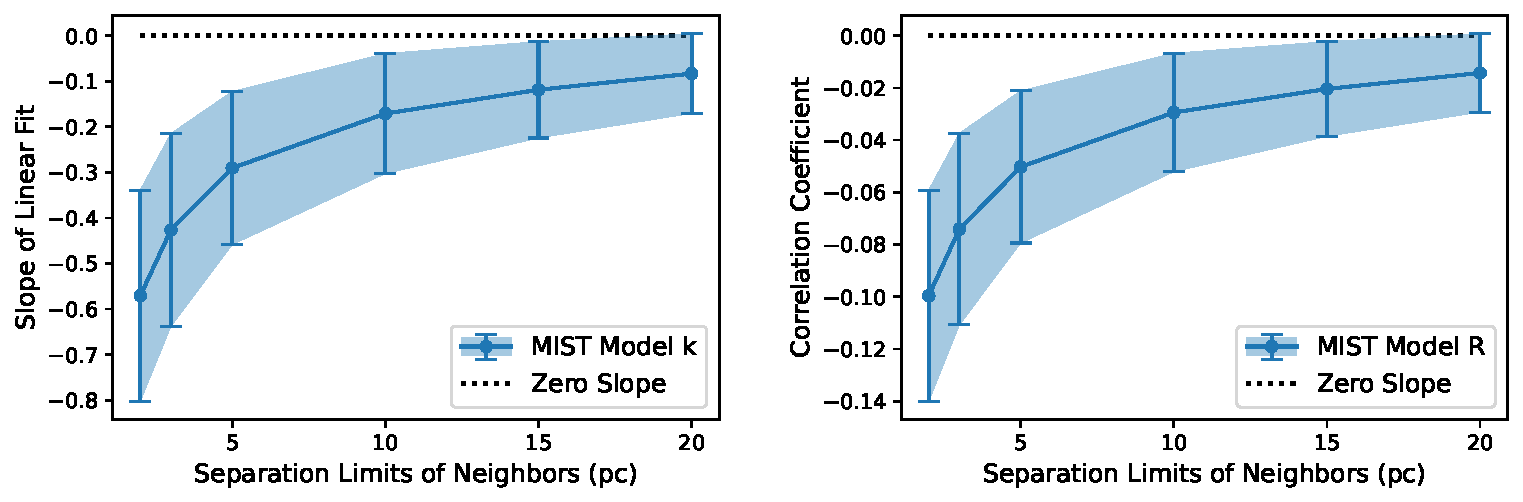
\includegraphics[width=\linewidth]{figures/chapter1/slope_vs_sep-simulate_dist.pdf}
    \caption[Parallax simulation results of the negative correlation between relative velocity and stellar mass]{Parallax simulation results of the slope of linear fit $k$ and correlation coefficient $R$ between relative velocity and stellar mass under the MIST model as a function of separation limits within which sources are considered as neighbors. The blue errorbar and the shaded region show the value and associated uncertainty of the two parameters, while the dashed line shows the zero slope, or no correlation.}
    \label{fig:simulate k R}
\end{figure*}


Previous analysis was conducted under the assumption that all of the sources are located at the exact same distance of $389\pm3$~pc for reasons discussed in Section~\ref{onc-subsec:3d velocities}. However, this is not the actual case, especially when we are considering the distances between neighboring sources. Seemingly adjacent sources on the plane of the sky might be distant from one another along our line of sight.

To investigate the impact of unknown distances to individual stars, we chose to simulate the parallax for all of our $235$ sources following the same distribution of the limited $100$ adopted \textit{Gaia} parallaxes. An inverse cumulative distribution function (CDF) is constructed from the $100$ parallax measurements. We then sample $235$ simulated parallaxes from the CDF and assign one value to each source. The simulation is repeated $1000$ times.

First, we present the simulation results on the correlation between relative velocity and stellar mass. The distance between sources is now updated to incorporate both the projection on the sky and the radial component. Figure~\ref{fig:simulate k R} shows the slope $k$ of the linear fit and correlation coefficient $R$ between relative velocity and stellar mass as a function of the separation limit within which we consider sources as neighbors. The blue errorbar and the shaded region represent the mean and standard deviation of the $1000$ simulated results of the slope $k$ and correlation coefficient $R$. As can be seen, the same increasing trend as the separation limit increases persists for both parameters, consistent with Figure~\ref{fig:slope_vs_mass}. Therefore, the conclusion remains based on the $1000$ parallax simulations: the negative correlation between relative velocity and stellar mass exists and becomes increasingly obvious when we consider the velocity relative to the more immediate neighbors of each source.



\begin{figure}[htb!]
    \centering
    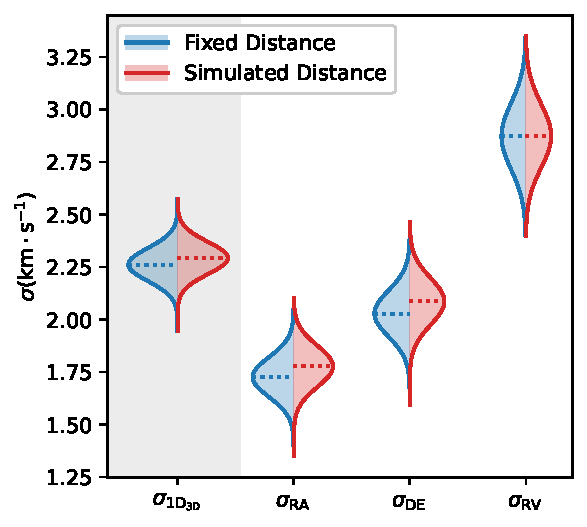
\includegraphics[width=0.7\linewidth]{figures/chapter1/vdisp_simulate.pdf}
    \caption[Comparison of velocity dispersions between the fixed distance scenario and the parallax simulation]{Comparison of velocity dispersions between the fixed distance scenario and the parallax simulation. The blue profile on the left of each column is a normal distribution of the velocity dispersion when every source is assumed at a fixed distance of $389\pm3$~pc, with the mean and the standard deviation specified as in Equation~\ref{eq:vdisp measurements}. The red profile on the right of each column shows the normalized summation of the $1000$ normal distributions of the velocity dispersions. We then fit a single normal distribution over the summed distribution, and the dashed lines show the mean of the normal distributions. The $\sigma_\mathrm{1D_{3D}}$ is shaded with a light gray background to visually distinguish from its components in all three directions.}
    \label{fig:vdisp simulate}
\end{figure}

Second, we report the velocity dispersion measurements in the parallax simulation. The same procedure of measuring the velocity dispersion is conducted in each simulation as in Section~\ref{onc-subsec:virial}. Each of the $1000$ simulations produces velocity dispersions and their associated uncertainties. To determine the final uncertainty of the simulation, we first add $1000$ normal distributions centering at the simulated values with the standard deviation being the uncertainties of each simulation and normalize it with a factor of $1/1000$. Then we fit a single normal distribution to the summation, and use the mean and standard deviation as the simulated values and uncertainties. The summation is justified because we are intrinsically assuming a normal posterior distribution of the parameters when we use a normal distribution likelihood function in the MCMC ensemble sampler. The simulated velocity dispersions are listed below:
\begin{align} \label{eq:vdisp simulation}
    \overline{\sigma}_\mathrm{RA} = 1.78\pm0.10~\mathrm{km}\,\mathrm{s}^{-1}, \nonumber \\
    \overline{\sigma}_\mathrm{DEC} = 2.09\pm0.11~\mathrm{km}\,\mathrm{s}^{-1}, \nonumber \\
    \overline{\sigma}_\mathrm{RV} = 2.87\pm0.15~\mathrm{km}\,\mathrm{s}^{-1}, \nonumber \\
    \overline{\sigma}_\mathrm{1D_{3D}} = 2.29\pm0.08~\mathrm{km}\,\mathrm{s}^{-1}.
\end{align}
A comparison of the velocity dispersions between the fixed and simulated distance scenarios is shown in Figure~\ref{fig:vdisp simulate}. As can be seen, the 1D velocity dispersion with simulated parallax is only slightly boosted by $0.03~\mathrm{km}\,\mathrm{s}^{-1}$ from the case of fixed distance, even smaller than the uncertainty. The change is mostly caused by a minute increase in the RA and DEC components, with the RV component remaining exactly the same. This proves that the projection effect cannot account for the higher $\sigma_\mathrm{RV}$ than the other $2$ directions. 

Additionally, the simulated virial ratio is $q=0.88$, only slightly different from the previous result of $0.85$. In summary, the projection on the plane of the sky does not have a significant effect on the velocity dispersion results.


\subsection{Mass Segregation and Energy Equipartition}
\label{onc-subsec:segregation}
\begin{figure*}[htb!]
    \centering
    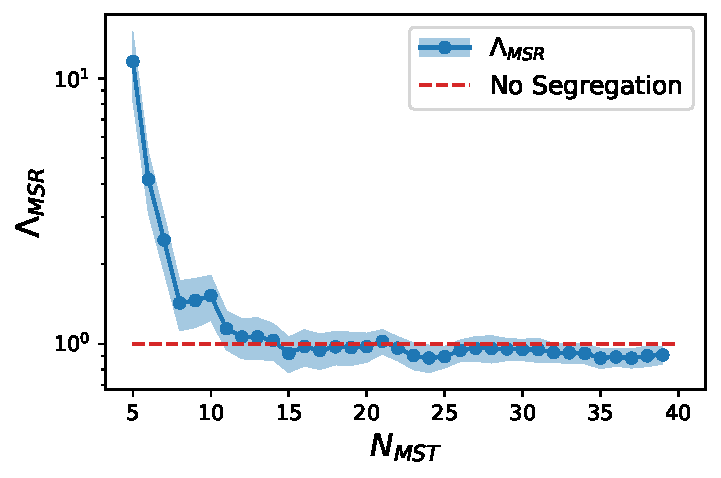
\includegraphics[width=0.496\linewidth]{figures/chapter1/MSR-MIST-all.pdf}
    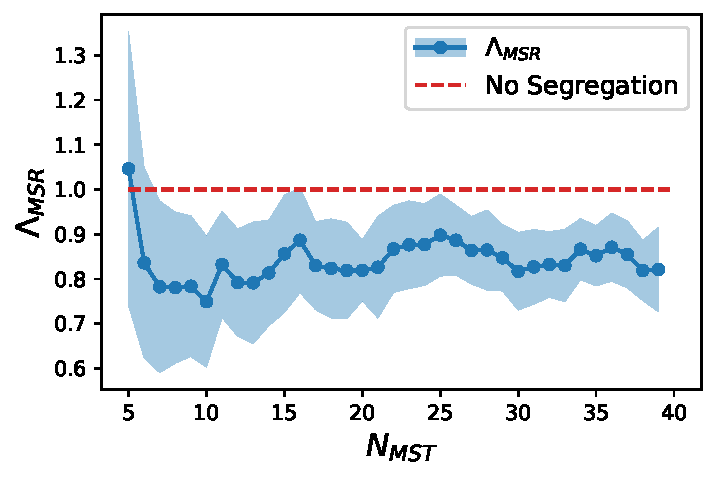
\includegraphics[width=0.496\linewidth]{figures/chapter1/MSR-MIST-no_trapezium.pdf}
    \caption[Mass segregation ratio with varying $N_\mathrm{MST}$]{Mass segregation ratio $\Lambda_\mathrm{MSR}$ under MIST model as a function of the number of sources chosen to construct the minimum spanning tree $N_\mathrm{MST}$. \textit{Left}: Including the Trapezium stars. \textit{Right}: Excluding the Trapezium star. Values greater than $1$ indicate mass segregation for the corresponding number of most massive stars, and inverse mass segregation for $\Lambda_\mathrm{MSR}$ less than $1$. The dividing line is shown in a dashed red line.}
    \label{fig:segregation}
\end{figure*}

% Brief intro
Mass segregation refers to the non-random distribution of stars in stellar systems, where more massive stars tend to concentrate toward the center while lower-mass stars are more dispersed in the outer regions. This occurs due to gravitational interactions and the differential response of stars of different masses to these interactions. Understanding mass segregation and its origin is essential for studying the evolution and formation of stellar systems \citep[e.g.,][]{Fregeau-2002, Baumgardt-2008}.

With stellar masses derived in Section~\ref{onc-subsec:mass}, the mass segregation in the central ONC can be quantified. Here we adopt the mass segregation ratio (MSR), $\Lambda_\mathrm{MSR}$, defined in \citet{Allison-2009}. This parameter uses the minimum spanning tree to measure how clustered the most massive stars in a cluster are. If the most massive stars tend to stay closer to each other compared to a random group of stars of the same amount, the ratio is larger than $1$, indicating mass segregation. Conversely, if the most massive stars are further away from each other than a random combination of stars, the ratio is less than $1$, or inversely mass segregated.

Figure~\ref{fig:segregation} shows the MSR under the MIST model as a function of $N_\mathrm{MST}$. Figure~\ref{fig:segregation}(a) shows our target sources combined with the high-mass Trapezium stars, while in Figure~\ref{fig:segregation}(b) the Trapezium stars are excluded to unveil the mass segregation for other stars. The dividing line of $\Lambda_{MSR}=1$ is plotted as a red dashed line in both figures. It is evident from Figure~\ref{fig:segregation}(a) that the $5$ most massive stars are very mass segregated, which is expected as the Trapezium stars are clearly spatially clustered in the ONC center.  We utilized the masses of the Trapezium stars from the literature (\citealt{Weigelt-1999, Close-2012} for $\theta^1$ Orionis A, \citealt{Vitrichenko-2006} for $\theta^1$ Orionis B, \cite{Balega-2014} for $\theta^1$ Orionis C, \citealt{Allen-2017} for $\theta^1$ Orionis D, and \citealt{Morales-Calederon-2012} for $\theta^1$ Orionis E). \citet{Hillenbrand-1998} argues that the high-mass stars are likely prone to form in the ONC center. Surprisingly, Figure~\ref{fig:segregation}(b) shows that the stars apart from the few Trapezium stars display a feature of inverse mass segregation, i.e., massive stars tend to be on the outskirts. This result may not be a true feature and could instead be a result of our sample selection. As mentioned previously, our goal in the NIRSPAO target selection was to obtain a good sampling of low-mass objects in the cluster core. The APOGEE sources are not preferentially sampled at low masses, tending to higher masses because of higher mass sensitivity limits at the $H$-band.  The APOGEE sources are also generally on the periphery of the region we are analyzing. Therefore, we may have missed some sources on the lower-mass end in the outskirts, which results in a bias in this result.  More complete spectra in the cluster core and outskirts are needed to assess whether this trend is real or a sample artifact.

While the most massive Trapezium stars in the cluster exhibit a close distribution around the cluster center, it is important to recognize that mass segregation does not necessarily indicate the occurrence of energy equipartition, as N-body simulation suggests \citep[][]{Parker-2016}. Instead, the kinetic energy decreases at the same rate for low and high-mass stars according to the simulation. This is consistent with our observation in that the stars with higher masses still have a slightly higher velocity dispersion, as can be seen from the left panel in Figure~\ref{fig:vdisp vs mass}.



\section{Conclusions}
\label{onc-sec:conclusion}
In this work, we present the 3D kinematic analysis of $235$ sources in the central region of the ONC, including $80$ sources observed by the Keck NIRSPAO and $167$ reanalyzed APOGEE sources, with $17$ common sources between the two surveys. High-precision radial velocities and effective temperatures, along with other stellar parameters, are retrieved from spectral analysis. With the help of previous proper motion measurements from HST and multiple stellar evolutionary models, we construct a 3D kinematic map of the region with interpolated stellar mass. Listed below are the main takeaways for this work.

\begin{enumerate}
    \item We model stellar parameters including $T_\mathrm{eff}$ and RV using high-resolution spectra from NIRSPAO ($R\sim25000$ or $35000$). Stellar masses are then derived from $T_\mathrm{eff}$ and four different stellar evolutionary models assuming a stellar age of $2\pm1$~Myr.

    \item The velocity dispersion in the right ascension, declination, radial direction are $\sigma_\mathrm{RA} = 1.73 \pm 0.09~\mathrm{km}\,\mathrm{s}^{-1},~\sigma_\mathrm{DEC} = 2.03 \pm 0.11~\mathrm{km}\,\mathrm{s}^{-1},~\sigma_\mathrm{RV} = 2.87 \pm 0.16~\mathrm{km}\,\mathrm{s}^{-1}$. The 1D velocity dispersion is $\sigma_\mathrm{1D_{3D}} = 2.26 \pm 0.08~\mathrm{km}\,\mathrm{s}^{-1}$, exceeding the requirement of virial equilibrium of $1.73~\mathrm{km}\,\mathrm{s}^{-1}$ \citep[][]{DaRio-2014}. Therefore, the ONC is not fully virialized yet, with a virial ratio of $0.85$, consistent with \citet{DaRio-2014}.

    \item A negative correlation between the velocity relative to the neighbors of each source and the stellar mass is identified using four different stellar evolutionary models, consistent with gravitational filament fragmentation simulation results. This suggests that during the star formation processes within infalling gas filaments, the high velocities of the fast-moving primordial stars preclude them from accreting more material from their surroundings.

    \item Neither the velocity dispersion nor the negative correlation is affected by the projection effect by assuming the same distance of $389\pm3$~pc for all sources. We conducted $1000$ simulations in which each source is assigned a simulated distance according to the distribution of the $100$ adopted \textit{Gaia} parallax measurements within our sample. The simulated IVD is consistent with the projected scenario, with $\sigma_\mathrm{RA}$, $\sigma_\mathrm{DEC}$, and $\sigma_\mathrm{1D_{3D}}$ slightly increased by less than $1\sigma$. The negative correlation still holds.
    
    \item There is a systematic discrepancy in the effective temperature between NIRSPAO and APOGEE results. The difference could be attributed to the different passbands used in the two instruments, $K$ and $H$ bands, respectively. The negative correlation between relative velocity and stellar mass still exists after accounting for the discrepancy by offsetting the NIRSPAO $T_\mathrm{eff}$ by the weighted-averaged difference. Furthermore, the negative correlation becomes more significant for more localized relative velocity.

    \item A clockwise rotational preference in proper motions is identified in the region.

    \item The sources are found to be inversely mass segregated, or massive stars being more scattered on the outskirts, if the Trapezium stars are excluded. This may stem from a selection bias as we are focusing on low-mass stars closer to the ONC center.

    \item We report $4$ binary candidate systems by observing the change in radial velocity, Parenago 1837, V* V1337 Ori, V*1279 Ori, and Brun 590. We were able to infer the properties of the companion with a mass most likely of $\sim0.03$--$0.3~M_\odot$ and a semi-major axis most likely of less than $2$~au.

    \item We simulate the effect of binaries have on the IVD in the radial component and conclude that binarity alone is insufficient to explain the higher value in IVD in the radial direction compared to the proper motion directions. Possible explanations are the interaction with the ISF, such as the slingshot mechanism, which states that the ONC is ejected from the ISF due to the oscillation of the gas filament \citep[][]{Stutz-2016, Stutz-2018, Matus-2023}.

    \item We calculate the expectation of the excess in mass contributed by unresolved close binaries within $10$~au. The expectation of the increase in mass is $8$--$14\%$. The negative correlation between relative velocity and stellar mass persists, albeit with a marginally flatter linear fit, after accounting for the contribution from unresolved binary mass. 

\end{enumerate}


In the future, we plan to construct kinematic maps in an extended area beyond our current $4\arcmin$ radius. This may place a tighter constraint on the current kinematic state of the larger cluster population, probing deeper into its formation history and implications. In addition, our observations are ideal first epochs for unresolved binary star searches, which will provide a true estimate of the very tight binary fraction in this region.


\facilities{HST(ACS/WFPC2/WFC3IR), SDSS(APOGEE), Keck}
\software{
    \texttt{astropy} \citep{Astropy-2013, Astropy-2018, Astropy-2022},
    \texttt{astroquery} \citep{astroquery},
    \texttt{smart} \citep{Hsu-2021-code, Hsu-2021-paper},
    \texttt{emcee} \citep{Foreman-Mackey-2013},
    \texttt{velbin}  \citep{Cottaar-2014, Foster-2015},
    \texttt{TheJoker} \citep{thejoker}
}


\section*{Acknowledgment}
Chapter~\ref{chapter:onc}, in full, is a reprint of the material as it appears in the Astrophysical Journal, \citealt*{Wei-2024}. The dissertation author was the primary investigator and author of this paper.

\chapter{Structure and Dynamics of the Young Massive Star Cluster Westerlund 1}
\label{chapter:wd1}

We present a structural analysis of the young massive star cluster Westerlund 1 (Wd1). With multi-epoch Hubble Space Telescope (HST) observations, we measure the proper motions of \num{10346} stars and determine their kinematic memberships by fitting a Gaussian mixture model to their proper motions. After correcting for extinction and completeness, we model the stellar density distribution and confirm the presence of an elongation with an eccentricity of $0.71$. The eccentricity decreases slightly with increasing mass. We fit the radial profile with the Elson, Fall, and Freeman model, observing a decrease in the core radius with increasing mass, indicative of weak but detectable mass segregation. This finding is further supported by a measured mass segregation ratio of $\Lambda_\mathrm{\rm MSR}=1.11\pm0.11$, only above $1$ by $1\sigma$, and slightly shorter minimum spanning tree length for higher mass bins. The cluster has a 1D velocity dispersion of $4.13 \pm 0.13~\mathrm{km}\,\mathrm{s}^{-1}$, suggesting it is subvirial. The subvirial state implies either exceptionally high star formation efficiency or inefficient stellar feedback caused by local gas expulsion before stars reach the cluster. The crossing time is $0.30$~Myr and the relaxation time is $0.26$~Gyr. Given the age of Wd1 of $10.7$~Myr, we expect evident mass segregation for stars more massive than $10~M_\odot$, which accounts for the minor mass segregation found in the mass range of $1.12$--$15.21~M_\odot$ in this work. This suggests the overall mass segregation in Wd1 is not primordial.

\section{Introduction}
\label{wd1-sec:introduction}

Young massive clusters (YMCs) are areas of intense star-forming activity and offer unique insight into star formation, cluster modeling, and the initial mass function (IMF) \citep{PortegiesZwart-2010}. YMCs exist within disparate environments, ranging from the Galactic Center to the Galactic disk. Investigating differences in their physical properties allows us to determine the dependence of star formation on initial conditions. Finding similarities would indicate which fundamental mechanisms prevail despite such perturbations.  

Westerlund 1 (Wd1) is one of the most massive young star clusters in the Galaxy. Discovered more than half a century ago~\citep{Westerlund-1961}, Wd1 is an ideal site to study a starburst environment in detail for its youth, proximity, and rich population of stars across a wide range of masses. Substantial efforts have been devoted to accurately determining the fundamental properties of Wd1, such as its age and distance, to improve our understanding of this cluster.
% Despite active studies, there remains substantial uncertainty about the age and distance of Wd1, both of which are critical in accurately constraining the properties of cluster members. 

% Distance
Recent studies based on Gaia EDR3 and eclipsing binary analysis have converged on a distance estimate for Wd1 of $4.0$--$4.3$~kpc \citep[][]{Beasor-2021, Navarete-2022, Negueruela-2022}. In contrast, \citet{Aghakhanloo-2020} and \citet{Aghakhanloo-2021} reported a significantly closer distance of $2.6$--$2.8$~kpc using Gaia DR2 parallax measurements, although these estimates are potentially subject to sample selection bias \citep[][]{Negueruela-2022}. With HST optical and infrared observations, \citet{Hosek-2018} reported a distance ranging from $4.1$--$5.2$~kpc depending on the cluster age.

% Age
The diverse stellar populations in Wd1 enabled a variety of proxies for cluster age estimation. Previously, \citet{Clark-2005} and \citet{Crowther-2006} independently concluded a cluster age of $3.5$--$5$~Myr according to the formation models of Wolf-Rayet (WR) stars and supergiants. \citet{Negueruela-2010} reported an age of $6.3$~Myr with isochrones fitting B supergiants at $4.5$--$5$~kpc. \citet{Beasor-2021} determined a pre-main-sequence (PMS) age of $7.2$~Myr, while the eclipsing binary W13 sets a minimum age of $5$~Myr, and the faintest red super giants (RSGs) suggest an older age of $10.4$~Myr. These age estimates were further supported by \citet{Navarete-2022} and \citet{Rocha-2022}, in which the authors proposed that the broad age spread may reflect multiple episodes of star formation within the cluster.

Accurate measurements of the cluster age and distance from the color-magnitude diagram (CMD) require modeling the kinematic and photometric membership and an extinction map.

As one of the most massive young clusters in the Milky Way, Wd1 is a benchmark for testing models of star cluster formation and evolution. Due to the limited photometric depth of previous studies, the initial cluster mass of Wd1 has been mostly derived by extrapolating a canonical IMF \citep[][]{Brandner-2008, Clark-2005, Andersen-2017}. This method suggested a cluster mass of $4-6\times10^4 M_\odot$, corresponding to a viral equilibrium velocity dispersion of $4$--$6\,\mathrm{km}\,\mathrm{s}^{-1}$. This estimate significantly exceeds the previously measured velocity dispersion of $2.1^{+3.4}_{-0.9}\,\mathrm{km}\,\mathrm{s}^{-1}$ \citep[][]{Cottaar-2012}, implying that Wd1 is subvirial and gravitationally bound, despite having dispersed most of its gas mass at an age of $\sim10$~Myr. The virial state directly impacts these models, influencing assumptions about initial conditions, gas expulsion, and feedback in massive clusters.

Uncertainties about the virial state of Wd1 persist due to the reliance on assumptions about its IMF. Currently, there are conflicting results on the high-mass slope of the IMF of Wd1, e.g., $\alpha=-2.44^{+0.08}_{-0.20}$ in the mass range $3.5$--$27~M_\odot$ by \citet{Gennaro-2011} and $\alpha=-1.8\pm0.1$ in the mass range $5$--$100~M_\odot$  by \citet{Lim-2013}. For low-mass stellar content, \citet{Andersen-2017} argued for the IMF in the cluster to be consistent with the canonical IMF for the mass range $0.15$--$1.4~M_\odot$. Recent studies have reported similarly unusual IMFs in other YMCs, such as the Galactic Center~\citep{Lu-2013} and the Arches cluster~\citep{Hosek-2019}, raising the question of whether these deviations are environmentally driven or are intrinsic to YMCs in general. Wd1 provides an excellent opportunity to test this. Kinematic membership is critical to remove the field star contamination, which could be high enough to inflate the slope of the IMF in the low-mass and substellar regimes. 

Mass segregation in Westerlund 1 offers critical insights into the cluster’s dynamical evolution and star formation history. However, contradicting results have also been reported on the mass segregation in Wd1. \citet{Gennaro-2011} argued that the cluster appears mass-segregated, based on the radial variations of the IMF slope.  \citet{Gennaro-2017} later revisited the cluster using the mass segregation ratio $\Lambda_{\rm MSR}$, and found little evidence of mass segregation for stars more massive than $3.5M_\odot$, except for the most massive stars above $40M_\odot$. The authors concluded that Wd1 was not primordially segregated. The different result from \citep{Gennaro-2011} is attributed to fitting IMF slopes involving rather arbitrary binning, which could bias toward a high degree of mass segregation \citep[][]{Gennaro-2017}. \citet{Cottaar-2012}

In this paper, we determine the kinematic and photometric cluster members of Wd1 using observations with multiple epochs and filters from the Hubble Space Telescope (HST). With an extinction map based on the main-sequence population in the cluster, we present its differentially dereddened, field-decontaminated CMDs in the mass range $1.12$--$15.21\,M_\odot$. We derive the radial profile of Wd1 and examine the degree of mass segregation using the cluster members.

This paper is structured as follows. Section~\ref{wd1-sec:observations} illustrates the observation details. Section~\ref{wd1-sec:data} introduces the extraction and calibration of the data.
Section~\ref{wd1-sec:methods} elaborates on the methods we use for modeling the properties of the cluster, including determining cluster membership for each source, the extinction map, and completeness. In Section~\ref{wd1-sec:results}, we present the main results, including the surface density, morphology, radial density profile, cluster age and distance, radial profile, velocity dispersion, and mass segregation. We discuss the elongation, virial state, radial profile comparisons, dynamical timescales, the origin of mass segregation, and their implications in Section~\ref{wd1-sec:discussion}. Finally, we summarize the conclusions in Section~\ref{wd1-sec:conclusion}.


\section{Observations}
\label{wd1-sec:observations}

\begin{figure}[htb!]
\centering
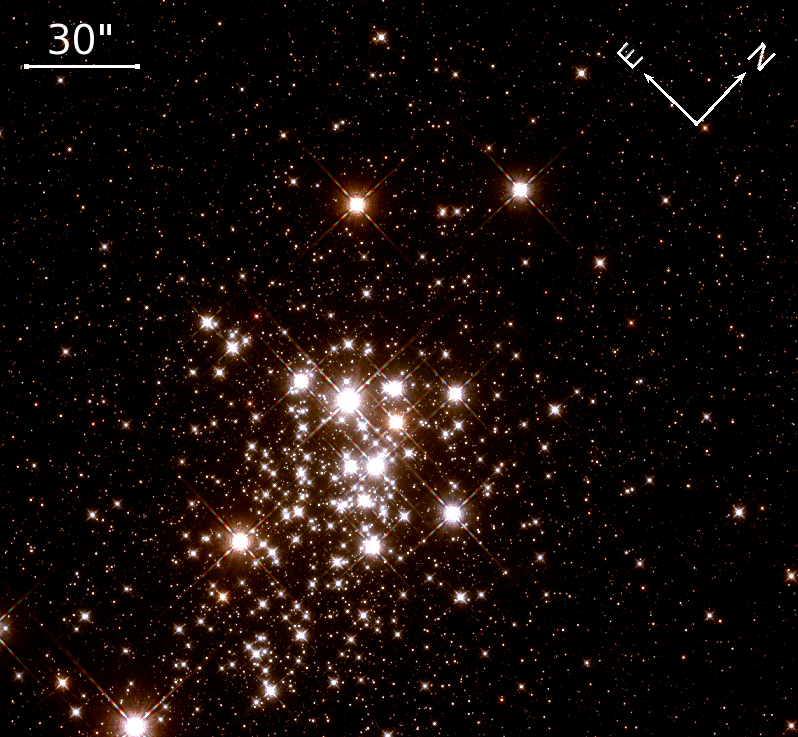
\includegraphics[width=0.7\linewidth]{figures/chapter2/wd1_rgb.png}
\caption[Hubble Space Telescope infrared image of Westerlund 1]{A Hubble Space Telescope WFC3-IR image of Westerlund 1 in false color. A logarithmic color stretch is used with red = F160W, green = F139M, and blue = F125W.}
\label{fig:wd1_rgb}
\end{figure}

Wd1 ($\mathrm{R.~A.}=16^\mathrm{h}\,47^\mathrm{m}\,05.57^\mathrm{s}$, $\mathrm{Dec.}=-45\deg\,50\arcmin\,24.14\arcsec$, J2000) was observed with the Hubble Space Telescope (HST) at multiple epochs to measure proper motions (PMs) and in multiple filters to obtain multi-color photometry. 
The cluster was observed at four different epochs --- 2005, 2010, 2013, and 2015 --- and in four filters at both red-optical and infrared wavelengths. 
See Figure~\ref{fig:wd1_rgb} for a composite image. 

The earliest data set was obtained on 2005 Jan 23 with the Advanced Camera for Surveys Wide Field Camera (ACS-WFC, GO-10172, \citealt{prop10172D}) using the F814W filter ($\lambda = 806\;\mathrm{nm}, \Delta\lambda = 287\;\mathrm{nm}$). 
The total exposure time was 2407 seconds, comprised of 3 images with small dithers to cover the chip gap. The final image covers a $211''\times218''$ field of view (FOV). 
In these individual optical exposures, stars brighter than $m_{\rm F814W}=18.4$ were saturated; however, astrometry and photometry can still be extracted for stars as bright as $m_{\rm F814W}=13$ with increased uncertainty. 

A second data set was obtained in 2010 with the infrared channel of the Wide Field Camera 3 (WFC3-IR) using three filters (GO-11708, \citealt{prop11708A}). Due to the limited FOV of WFC3-IR $\sim130''$, a $2\times2$ mosaic was used to cover the entire 2005 ACS-WFC FOV. The three infrared filters were  F125W ($\lambda = 1249\;\mathrm{nm}, \Delta\lambda = 285\;\mathrm{nm}$),  F139M ($\lambda = 1384\;\mathrm{nm}, \Delta\lambda = 64\;\mathrm{nm}$),  F160W ($\lambda = 1537\;\mathrm{nm}, \Delta\lambda = 268\;\mathrm{nm}$). Seven images per filter were observed at each point in the mosaic. The total exposure times for each tile were $2444$~s in the F125W filter, 6294 s in the F139M filter, and 2094 s in the F160W filter, where each tile comprised 7 images. 

A third and fourth data sets were obtained in 2013 (GO-13044, \citealt{prop13044L}) and 2015 (GO-13809, \citealt{prop13809L}) with WFC3-IR in the F160W filter to provide multi-epoch astrometry for sources detected at infrared wavelengths. The position angle of the 2013 and 2015 WFC-IR data was rotated $\sim$180$^\circ$ with respect to the position angle of the 2010 WFC3-IR data. Two short $8$~s exposures were added to provide further information on the brightest stars in case the saturation and errors were unacceptable in the long exposures. Details of the exposure times, number of exposures, and sensitivity of each filter are presented in Table~\ref{wd1-tab:observations}.


\begin{deluxetable}{llrrccrrr}
\tablecaption{Wd1 Observations from HST}
\label{wd1-tab:observations}
\tablewidth{0pt}
\tabletypesize{\scriptsize}
\tablehead{
    \colhead{Date\tablenotemark{a}} & 
    \colhead{Filter} & 
    \colhead{P.A.} &
    \colhead{t$_{exp}$\tablenotemark{b}} & 
    \colhead{N$_{\mathrm{img}}$\tablenotemark{c}} & 
    \colhead{N$_{\mathrm{dith}}$} & 
    \colhead{N$_{\mathrm{stars}}$} & 
    \colhead{$\sigma_{\mathrm{trans}}$} & 
    \colhead{HST ID} 
    \\
    \colhead{} & 
    \colhead{} &
    \colhead{(deg)} &
    \colhead{(s)} & 
    \colhead{} &
    \colhead{} & 
    \colhead{} &
    \colhead{(mas)} &
    \colhead{}
}
\startdata
2005.485 & F814W &   46.43 & 802 &  3 & 1          & 10,056 & 0.30 & 11708 \\
2010.652 & F125W &  -45.87 & 349 &  7 & 2$\times$2 & 10,029 & 0.91 & 11708 \\
2010.652 & F139M &  -45.87 & 899 &  7 & 2$\times$2 & 10,028 & 0.92 & 11708 \\
2010.652 & F160W &  -45.87 & 299 &  7 & 2$\times$2 & 10,056 & 0.85 & 13044 \\
2013.199 & F160W &  134.67 & 299 & 14 & 2$\times$2 & 10,056 & 0.89 & 13044 \\
2013.202\tablenotemark{d} 
         & F160W &  134.67 &   8 &  1 & 8$\times$8 &  6,571 & 0.19 & 13044 \\
2015.148 & F160W &  134.67 & 249 & 13 & 2$\times$2 & 10,056 & 0.86 & 13809 \\
2015.149\tablenotemark{d} 
        & F160W &  134.67 & 8 & 1 & 8$\times$8 & 6,571 & 0.18 & 13809
\enddata
\tablenotetext{a}{Images were taken over the course of 2 days. The date used in the PM analysis is the average over the individual images.}
\tablenotetext{b}{Exposure time for a single image.}
\tablenotetext{c}{Number of images at each dither position.}
\tablenotetext{d}{These data were sub-arrayed to one-quarter of 
the detector.}
\end{deluxetable}

The data were reduced using the standard online HST data reduction pipeline, and the resulting FLT images (\texttt{*\_flt.fits}) were downloaded from the HST archive.
All astrometric and photometric measurements were extracted from the individual FLT images and then combined as described in Section~\ref{wd1-subsec:astrometry_photometry}. 
The drizzle combined DRZ images (\texttt{*\_drz.fits}) for each filter and epoch were used to calibrate the photometric zeropoints.


\section{Data Analysis}
\label{wd1-sec:data}
\subsection{Astrometric and Photometric Extraction}
\label{wd1-subsec:astrometry_photometry}

We construct an astrometric and photometric catalog for each HST data set as follows. 

\begin{enumerate}[leftmargin=*, label=\roman*., align=left, labelsep=0em, itemsep=0em]
\item Extract star lists of stellar positions and fluxes for each image
\item Cross-match star lists and transform them into a common astrometric reference frame
\item Combine astrometric and photometric measurements for all images within an epoch, in order to estimate average positions, fluxes, and associated errors.  
\end{enumerate}

The final product is a catalog for each epoch and filter of stellar fluxes in instrumental magnitudes and positions in pixels in a camera coordinate system. 
Instrumental fluxes are converted to Vega magnitudes as described in Section~\ref{wd1-subsec:photometric_calibration}. 
Each step is described in more detail below. 

First, stellar fluxes and positions are initially extracted from the individual \texttt{flt} images using point spread function (PSF)-fitting methods and the \texttt{HST1PASS} software adapted from \citet{Anderson-2022}.  During the source extraction process, the known camera distortions are corrected for both ACS-WFC and WFC3-IR\footnote{The WFC3-IR distortion solution can be downloaded from \url{https://www.stsci.edu/files/live/sites/www/files/home/hst/instrumentation/wfc3/data-analysis/psf/_documents/STDGDC_WFC3IR.fits}} \citep{Anderson-2006}.

We derive the first-order coordinate transformations of all the star lists with \texttt{HST1PASS}, based on 2005 ACS-WFC F814W data as an initial reference frame, which has the finest resolution. Reference stars are chosen to fall within $0.07$ ACS pixels or $3.5$~mas and have an instrumental F814W magnitude between $-13.5$ and $-10.0$. Uncertainties on positions and fluxes are derived from the root-mean-squared (RMS) error of the measurements in the individual exposures and are typically below $0.5$~mas for the brightest stars. This process is repeated using the averaged star list from the first pass as a new reference frame and using more faint stars in the transformation. We note that the 2005 ACS-WFC F814W star list is also transformed to treat the two chips as independent images, each with its own transformation. This second pass reduces uncertainties by a factor of four to $0.006$ ACS pixels, or $0.3$~mas.

Preliminary PMs are determined by identifying cluster members, which are then used to establish a refined set of reference stars. The reference stars are selected based on the following properties: 
\begin{enumerate}[leftmargin=*, label=\roman*., align=left, labelsep=0em, itemsep=0em]
    \item Preliminary PMs within $0.7~\rm mas\,yr^{-1}$ of the cluster's mean motion;
    \item Preliminary PM uncertainties less than $0.2~\rm mas\,yr^{-1}$;
    \item Photometric uncertainties of less than $5\%$ in F814W and $10\%$ in the IR passbands.
\end{enumerate}
The entire process of transforming individual exposures is repeated with the new reference frame. The final transformation residuals are listed in Table~\ref{wd1-tab:observations} for each epoch and filter.

With the image coordinate transformations in hand, we use the sophisticated source detection routine \kstwo~\citep{Anderson-2006, Anderson-2008, Bellini-2017, Bellini-2018} to extract stellar fluxes and positions from a stack of images, which results in a much deeper catalog. The positions and fluxes of these stars are measured from the individual image using the individual-image PSFs described earlier. 

The positions of stars from each exposure are averaged within each epoch, and uncertainties of positions and fluxes are estimated in the same manner as described above. Figure~\ref{fig:astrometric_error} and Figure~\ref{fig:photometric_error} show the final astrometric and photometric RMS errors, respectively, for all stars in the catalog. 

\begin{figure}[htb!]
\centering
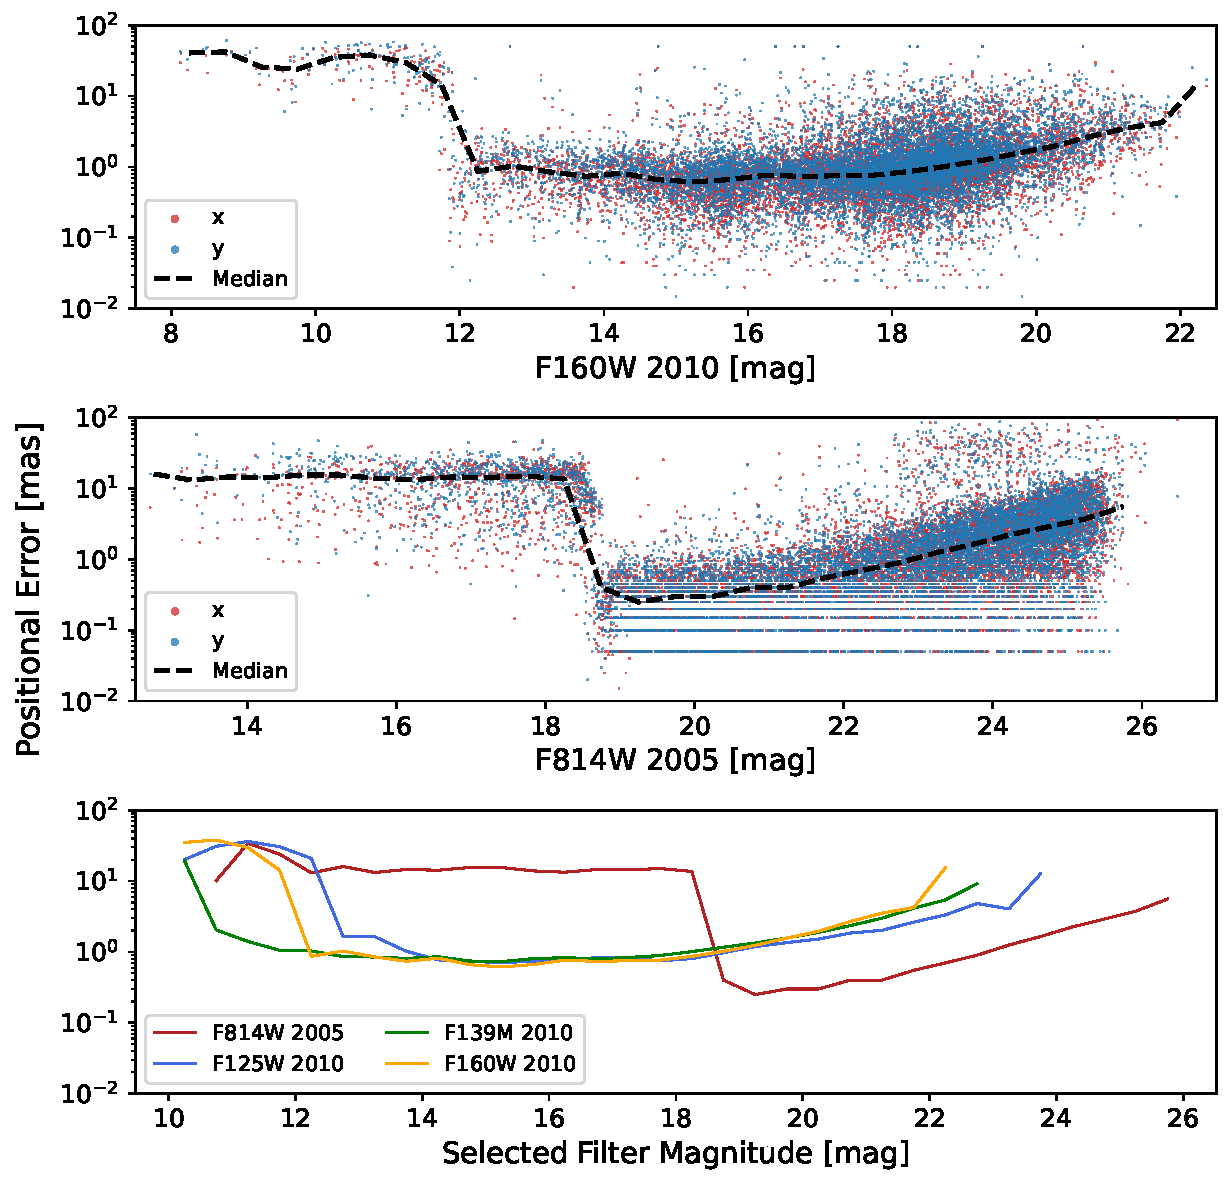
\includegraphics[width=\linewidth]{figures/chapter2/WD1_Positional_Errors_no_title.pdf}
\caption[Wd1 astrometric error vs. brightness]{Astrometric error vs. brightness for all filters and years. The astrometric error is the RMS error over the individual exposures in each filter and epoch. The errors in $x$ ({\em red}) and $y$ ({\em blue}) are oriented along the detector coordinates of the 2005 F814W observations. The {\em dashed black} lines in the first two panels show the median error after rejecting outliers larger than $3\sigma$. The {\em bottom} panel shows the median error line for all the filters and years.}
\label{fig:astrometric_error}
\end{figure}


\subsection{Photometric Calibration}
\label{wd1-subsec:photometric_calibration}

The final catalogs are photometrically recalibrated since the published zeropoints for ACS-WFC and WFC3-IR are derived from aperture photometry rather than PSF fitting. 
We calculate a new photometric zeropoint for each filter with the following procedure: First, we download the drizzle-combined mosaics from the HST archive and perform aperture photometry on the images using an aperture radius of 0\farcs4 for the WFC3-IR images and 0\farcs5 for the ACS images. 
The apparent magnitudes for the stars in the drizzled images were determined using the Space Telescope Science Institute's published 2012 photometric zeropoints with $R=0.4$ aperture for WFC3-IR filters\footnote{\url{https://www.stsci.edu/hst/instrumentation/wfc3/data-analysis/photometric-calibration/ir-photometric-calibration}}, and 2005 zeropoint for F814W\footnote{\url{https://acszeropoints.stsci.edu}}.

We cross-match stars between our final catalogs from \texttt{ks2} and the drizzled-image starlists. 
A set of photometric calibration stars is selected to be bright but not saturated in the instrumental magnitude range of $-11.0$ to $-9.5$ and to be isolated with no neighbors of comparable magnitudes within $0.25$~mas. These stars are used to derive the average flux ratio and new zeropoints for our PSF photometry.  Table~\ref{wd1-tab:zeropoints} contains the zeropoints for both 2012 photometric calibration with $R=0.4$ aperture and \texttt{ks2} photometry for all filters.

\begin{figure}[htb!]
\centering
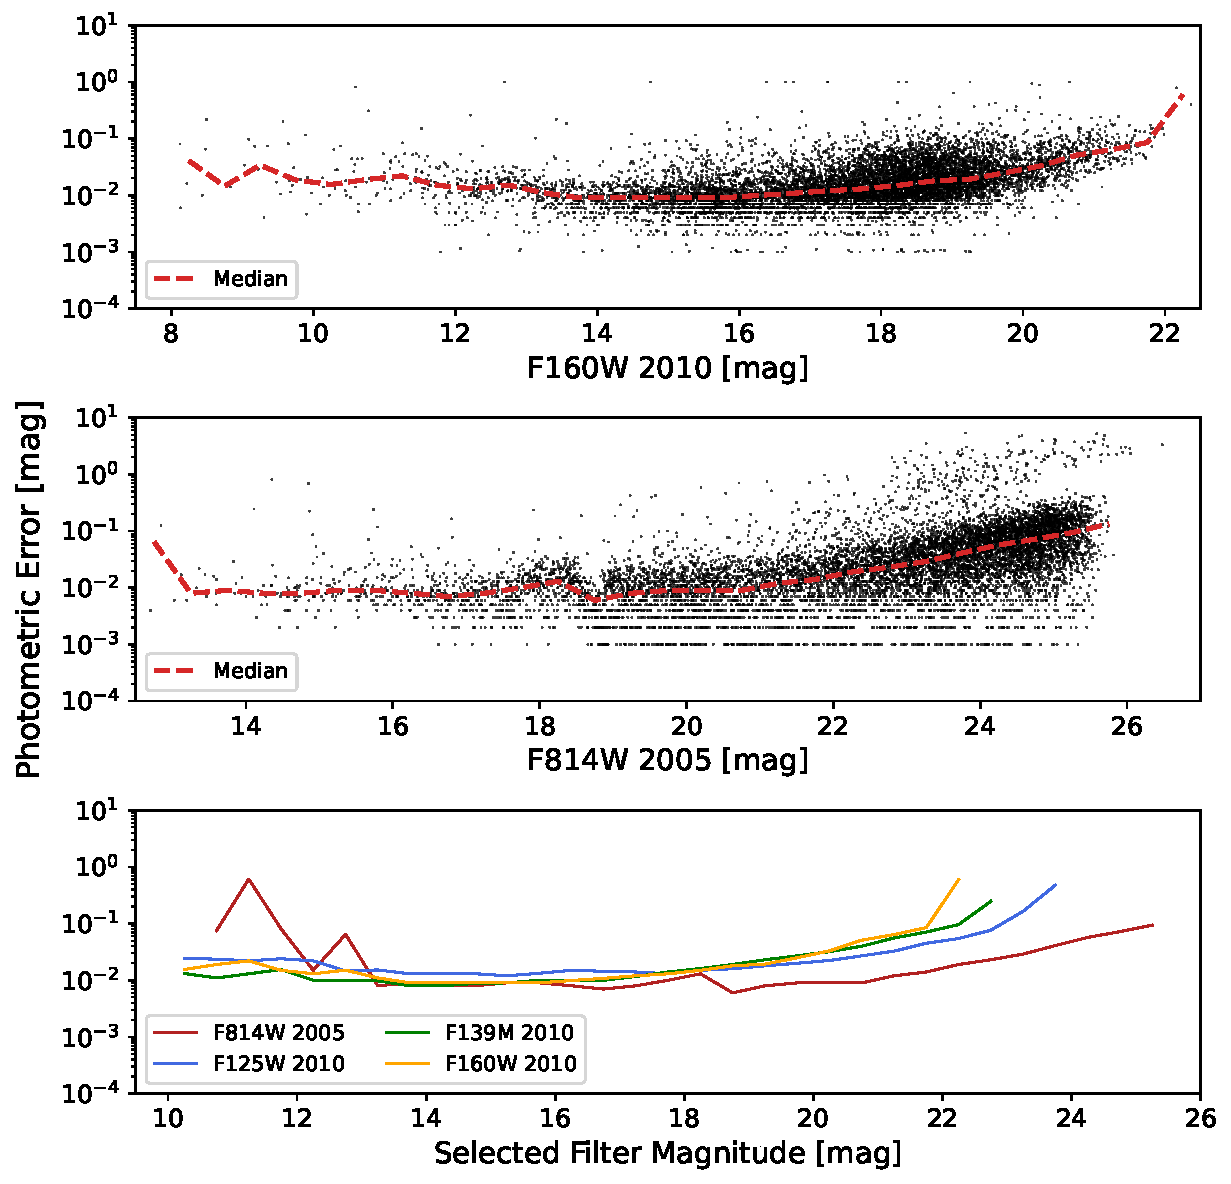
\includegraphics[width=\linewidth]{figures/chapter2/WD1_Photometric_Errors_no_title.pdf}
\caption[Photometric error vs. magnitude]{Photometric error vs. brightness for selected filters and years. The photometric error is the RMS error over the individual exposures in each filter and year. The {\em dashed red} lines in the first 2 panels show the median error after rejecting large ($>3\sigma$) outliers. The {\em bottom panel} shows the optical and representative infrared filters/years.}
\label{fig:photometric_error}
\end{figure}


\begin{deluxetable}{lcr}
\tablewidth{0pt}
\tabletypesize{\scriptsize}
\tablecaption{Photometric Zeropoints}
\label{wd1-tab:zeropoints}
\tablehead{
\colhead{} & \multicolumn{2}{c}{Zeropoints (mag)}\\
\colhead{Filter} &
\colhead{Aperture\tablenotemark{a}} &
\colhead{\kstwo} 
}
\startdata
F814W & $25.518$ & $32.678 \pm 0.010$ \\
F125W & $25.144$ & $25.231 \pm 0.010$ \\
F139M & $23.209$ & $23.284 \pm 0.010$ \\
F160W & $24.504$ & $24.570 \pm 0.010$ \\
\enddata
\tablenotetext{a}{2005 zeropoint value for F814W and 2012 photometric calibration values $R=0.4$ aperture for F125W, F139W, F160W.}
\end{deluxetable}

\subsection{Final Proper Motions}
\label{wd1-subsec:proper_motions}

% red.make_catalog(use_RMSE=True, vel_weight='error')
PMs are derived with the linear fit on astrometric positions for stars detected in all four epochs, including 2005 F814W, 2010 F160W, 2013 F160W, and 2015 F160W observations:
\begin{align}
    \alpha^* &= \mu_{\alpha^*}(t - t_0) + \alpha_0^*\\
    \delta &= \mu_\delta(t - t_0) + \delta_0\,,
\end{align}
where $t_0$ is the average time weighted by the inverse square of the astrometric uncertainties, $\left(\alpha^*, \delta\right)$ is the observed position at time $t$, and $\left(\alpha_0^*, \delta_0\right)$ is the position at reference time $t0$. We adopt the flattened RA $\alpha^*=\alpha\cos{\delta}$ in this study. PMs are fit to the positions weighted by the inverse square of the positional error in each epoch \citep[see][for a more complete description]{Ghez-2005, Lu-2009, Yelda-2014, Hosek-2015}. The resulting observed catalog contains \num{10346} stars with PMs and associated uncertainties. 

Rather than instituting a PM error cut on the resulting catalog, we opt to exclude stars with PMs exceeding $3\sigma$ from the median in both $x$ and $y$ directions (Figure~\ref{fig:box_cut_vpd}). We institute the box cut to ensure that our membership selection process is not hampered by stars in the extreme edges of the PM distribution. This cut removes \num{344} stars from the catalog. The catalog contains \num{10002} stars for the PM membership analysis.

\begin{figure}[htb!]
\centering 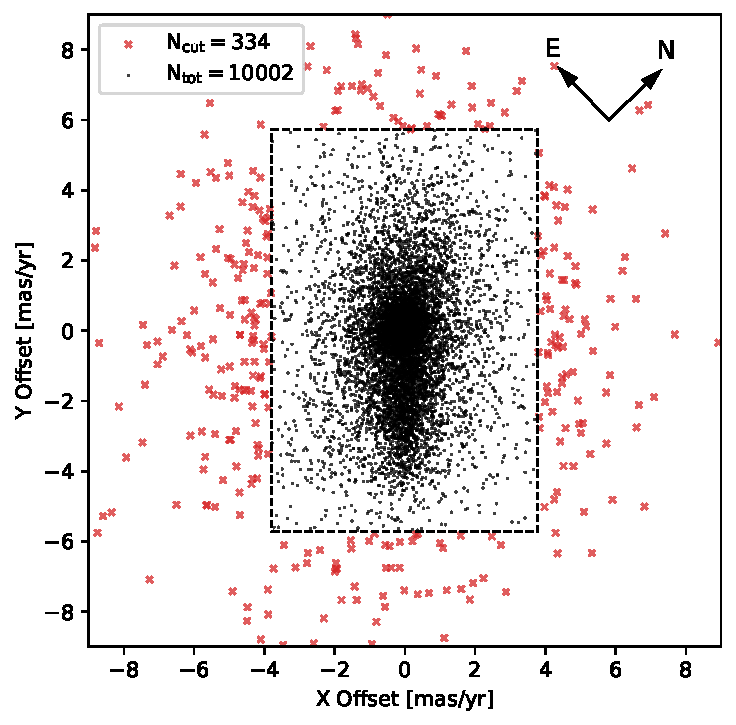
\includegraphics[width=0.7\linewidth]{figures/chapter2/WD1_Proper_Motion_Membership_no_title_w_ne.pdf}
\caption[Proper motion vector point diagram of Wd1]{Proper motion vector point diagram of the entire catalog. The central box outlined by the black dashed lines shows the $3\sigma$ cut in both directions. The kept stars are marked in black points inside the box, and the cut stars are marked in red crosses outside the box.}
% about the cluster bulk motion to prevent outliers from weighting the multi gaussian mixture model fit.
\label{fig:box_cut_vpd}
\end{figure}



\section{Methods: Modeling the Cluster}
\label{wd1-sec:methods}

\subsection{Cluster Membership}
\label{wd1-subsec:cluster_membership}

\begin{figure*}[htb!]
\centering
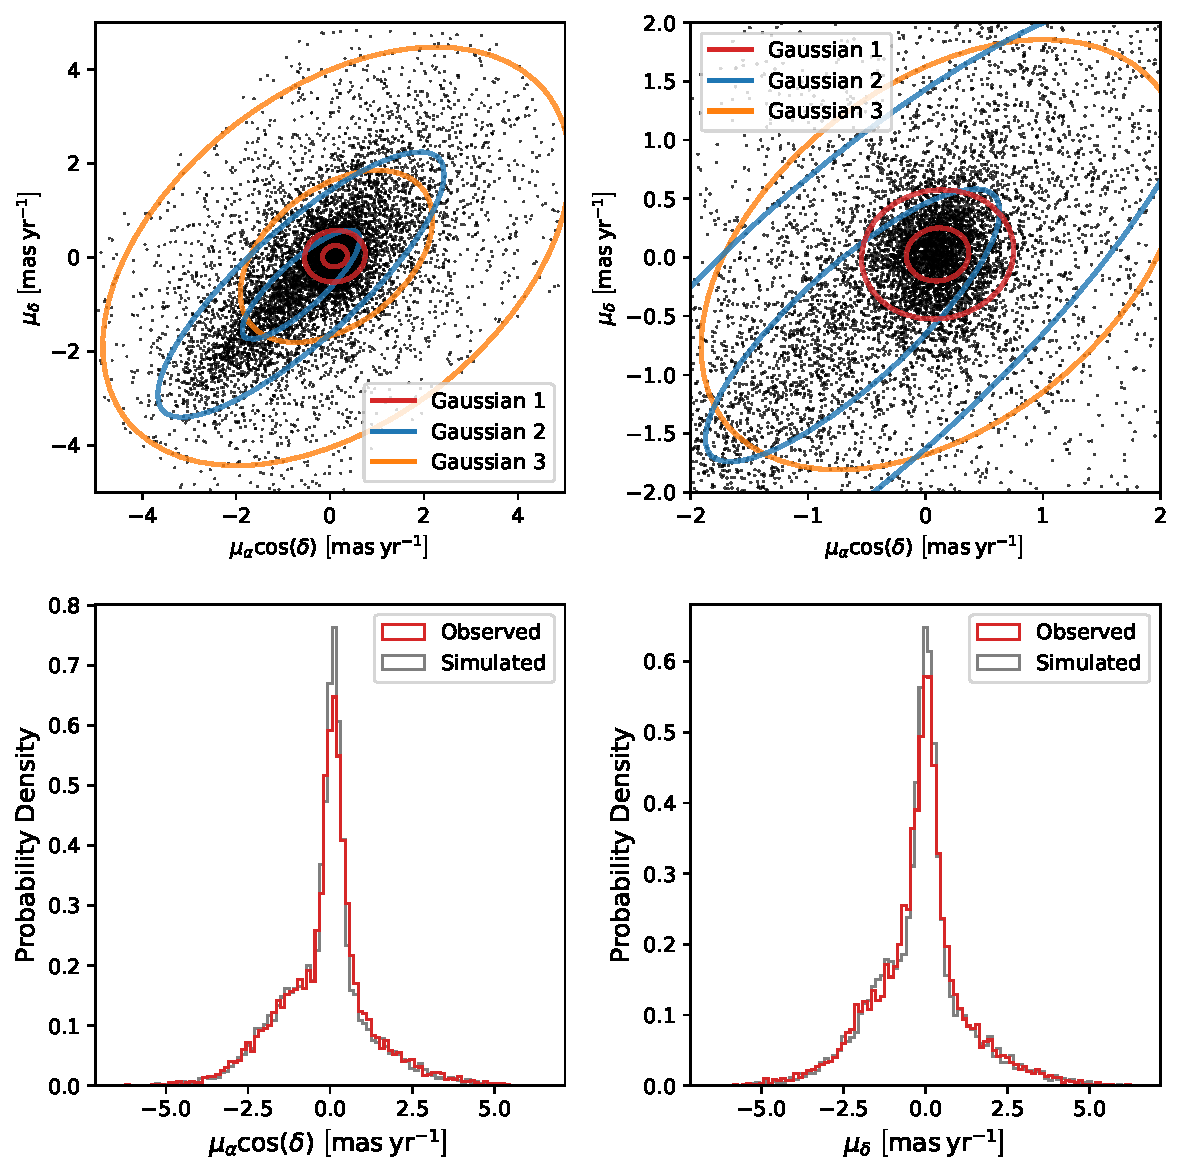
\includegraphics[width = \linewidth]{figures/chapter2/4_panel_VPD_Distributions.pdf}
\caption[Gaussian mixture model fit and probability densities of the proper motions]{GMM fit and probability densities of the PMs. \emph{Top}: Three-component GMM fit of the PMs shown in the \emph{top left} panel and a zoomed-in view on the \emph{top right} panel. Each Gaussian model is shown in its $1\sigma$ and $3\sigma$ iso-density ellipses. The first Gaussian depicted in red models the probability of being a cluster member, while the second and third Gaussian, shown in blue and amber, respectively, models the field star probabilities. \emph{Bottom}: Probability density distributions of PMs in the RA direction shown in the \emph{bottom left} panel and DEC direction in the \emph{bottom right} panel. Observed stars and simulated stars, assuming the GMM perfectly describes their PM, are shown in red and gray, respectively.}
\label{fig:wd1_vpd_distribution}
\end{figure*}


\begin{figure*}[htb!]
\centering
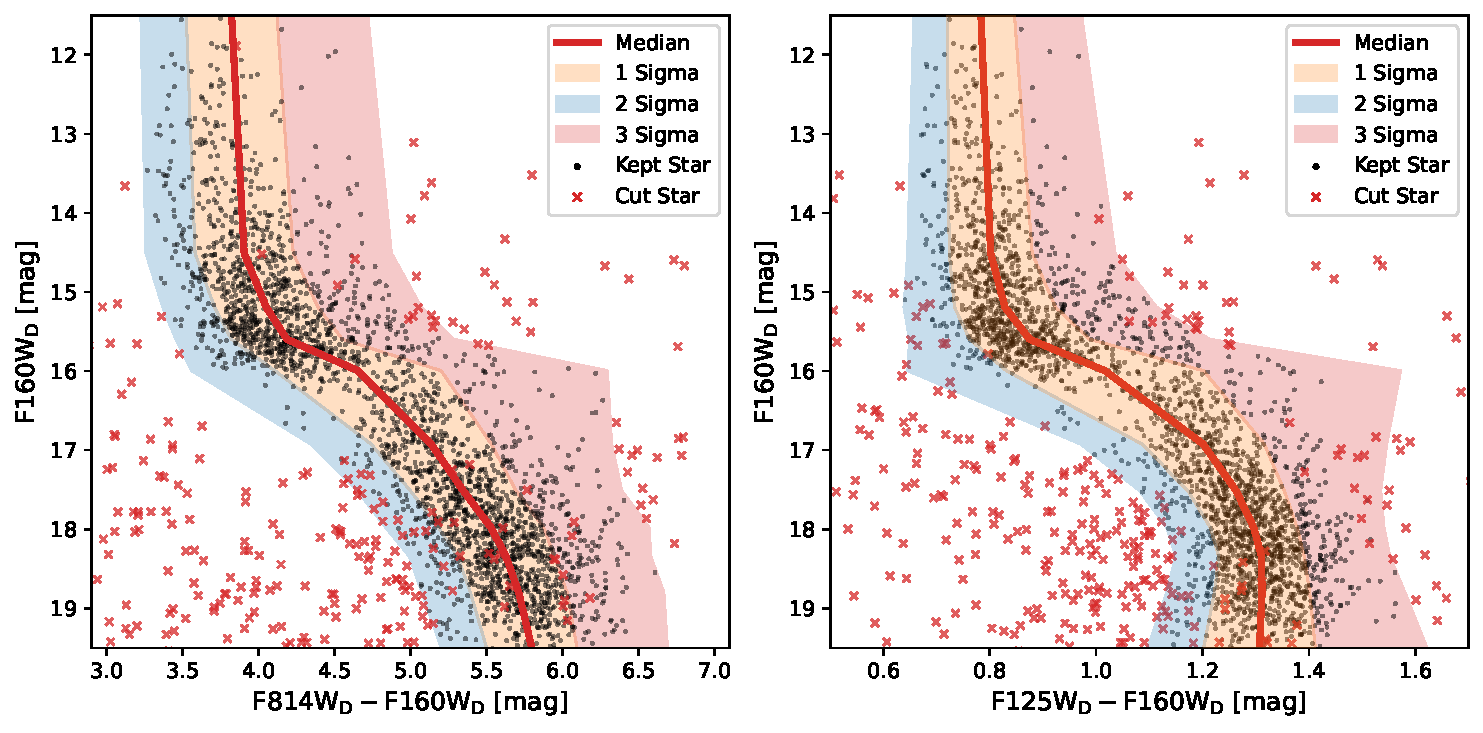
\includegraphics[width = \linewidth]{figures/chapter2/color_plot_bsig_2_rsig_3_m_11_20_bmarked_False.pdf}
\caption[Color membership of Wd1]{Color membership determination CMD's for F814W$-$F160W (\emph{left}) and F125$-$F160W (\emph{right}). The yellow-shaded region represents $1$--$\sigma$ from the median. The blue and red shaded regions correspond to stars less than $2$--$\sigma$ bluer and $3$--$\sigma$ redder than the median, respectively. Stars $2$--$\sigma$ bluer or $3$--$\sigma$ redder than the median in each magnitude bin, or, equivalently, those outside any shaded regions, are excluded from our final analysis. Stars marked in red crosses are the cut stars, while black dots are the kept ones. Here, the bins have been adaptively sized to contain approximately $287$ stars in each of the $10$ bins. Contaminating objects within our restricted cluster sequence may be binaries or field stars.}
\label{fig:color_membership}
\end{figure*}


\begin{figure}[htb!]
\centering 
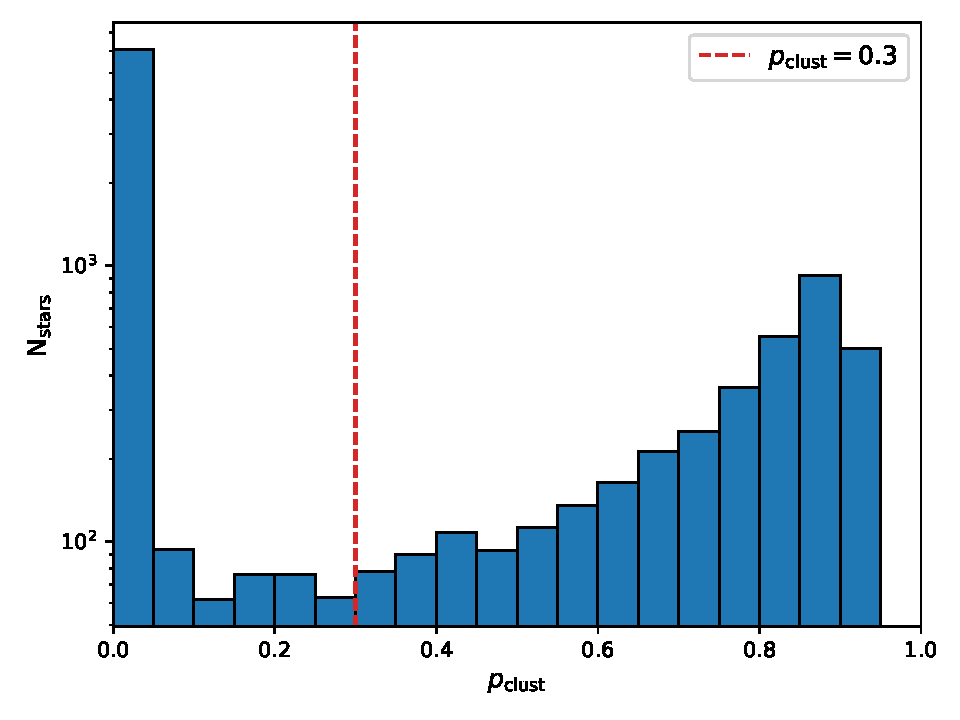
\includegraphics[width = 0.7\linewidth]{figures/chapter2/membership_histogram.pdf}
\caption[Histogram of Wd1 cluster membership probability]{Histogram of Wd1 cluster membership probability $p_{\mathrm{clust}}$ = $p_\mu \cdot p_{\mathrm{color}}$. The {\em red dashed line} line marks the cluster membership limit of $p_\mathrm{clust} = 0.3$. }
\label{fig:mem_histogram}
\end{figure}


We distinguish cluster members from contaminating field stars by analyzing the PM distribution and CMD. Each star in the catalog is assigned a PM membership probability, $p_\mu$, and a color membership probability according to its location in the CMD space, $p_{\mathrm{color}}$. The PM membership $p_\mu$ is a continuous variable that ranges from $0$ to $1$, whereas $p_{\mathrm{color}}$ is a boolean criterion. The final membership value is the product of the two components, $p_{\mathrm{clust}}$ = $p_\mu \cdot p_{\mathrm{color}}$.  Only stars with $p_{\mathrm{clust}} \geq 0.3$ are included in the structure and radial profile analysis. 

First, we determine the PM membership. As cluster members tend to move with a systemic PM, they can be distinguished from the field populations kinematically and should form a compact region on the vector point diagram (VPD), a diagram showing the PM vectors in the $x$ and $y$ directions, respectively. To robustly identify the cluster members in the region, we adopt a Gaussian Mixture Model (GMM) to model the PM distribution of cluster and field stars with Bayesian inference. This model allows us to assign a kinematic cluster membership probability to each star based on its PM. The model employs a mixture of $N$ Gaussians to represent the cluster and field star populations \citep[see][for details]{Clarkson-2012, Hosek-2015, Rui-2019}, with $N$ ranging from $2$ to $5$ explored in this analysis. We define the likelihood function for the set of $N$ measured stars, $\mathcal{L}$: 
\begin{equation}
    \mathcal{L} = \prod_i^N L(\mu_i)\,,
\end{equation}
where $L(\mu_i)$ is the likelihood of the $i$-th star with a measured PM vector $\boldsymbol{\mu}_i \equiv \left(\mu_{\alpha^*}, \mu_\delta\right)$, defined as:
\begin{equation}
    L(\mu_i) = \sum_{k=0}^K \frac{\pi_k}{2\pi|\Sigma_{ki}|^\frac{1}{2}}\exp{\left[-\frac{1}{2}(\boldsymbol{\mu}_i - \bar{\boldsymbol{\mu}}_k)^\top\Sigma_{ki}^{-1}(\boldsymbol{\mu}_i - \bar{\boldsymbol{\mu}}_k)\right]}
\end{equation}
for $K$ Gaussian components, where $\pi_k$ is the fraction of stars in the $k$-th Gaussian, $\bar{\boldsymbol{\mu}}_k$ is the PM centroid vector of the $k$-th Gaussian, $\Sigma_{ki}$ is the covariance matrix of the $k$-th Gaussian and the $i$-th star with a PM measurements of $\boldsymbol{\mu}_i$ and an associated uncertainty of $\boldsymbol{\epsilon}_i \equiv \left(\epsilon_{\alpha^*, i}, \epsilon_{\delta, i}\right)$. Following \citet{Hosek-2015} and \citet{Clarkson-2012} we take 
\begin{equation}
    \Sigma_{ki} = S_i + Z_k\,,
\end{equation}
where $S_i$ is the diagonal component of the velocity error matrix
\begin{equation}
    S_i = \begin{bmatrix}
        \epsilon_{\alpha^*, i}^2 & 0 \\
        0 & \epsilon_{\delta, i}^2
    \end{bmatrix}\,,
\end{equation}
and $Z_k$ is the covariance matrix of the $k$-th Gaussian component:
\begin{equation}
    Z_k = \begin{bmatrix}
        \sigma_{\alpha^*}^2 & \rho\sigma_{\alpha^*}\sigma_\delta \\
        \rho\sigma_{\alpha^*}\sigma_\delta & \sigma_\delta^2
    \end{bmatrix}~.
\end{equation}
Here $\sigma_{\alpha^*, i}$ and $\sigma_{\delta, i}$ denote the intrinsic velocity dispersion in the right ascension (RA) converted by $\cos{\delta}$ and declination (DEC) direction, respectively, and $\rho$ denotes the correlation coefficient between the two components.

With the likelihood function, the posterior probability distribution is determined by the Bayes' theorem: 
\begin{equation}
    P\left(\boldsymbol{\pi}, \bar{\boldsymbol{\mu}}, \boldsymbol{Z}|\boldsymbol{\mu}, \boldsymbol{S}\right) = \frac{P\left(\boldsymbol{\mu}, \boldsymbol{S}|\boldsymbol{\pi}, \bar{\boldsymbol{\mu}}, \boldsymbol{Z}\right) P\left(\boldsymbol{\pi}, \bar{\boldsymbol{\mu}}, \boldsymbol{Z}\right)}{P\left(\boldsymbol{\mu}, \boldsymbol{S}\right)}\,,
\end{equation}
where $P\left(\boldsymbol{\pi}, \bar{\boldsymbol{\mu}}, \boldsymbol{Z}|\boldsymbol{\mu}, \boldsymbol{S}\right)$ is the posterior probability of the model, $P\left(\boldsymbol{\mu}, \boldsymbol{S}|\boldsymbol{\pi}, \bar{\boldsymbol{\mu}}, \boldsymbol{Z}\right)$ is the probability of the observed velocity distribution given the model, $P\left(\boldsymbol{\pi}, \bar{\boldsymbol{\mu}}, \boldsymbol{Z}\right)$ is the prior probability of the model, and $P\left(\boldsymbol{\mu}, \boldsymbol{S}\right)$ is the sample evidence. 
Here, $\boldsymbol{\pi}$ is the set of $\pi_k$ values, $\bar{\boldsymbol{\mu}}$ the set of Gaussian velocity centroids, $\boldsymbol{Z}$ is the set of Gaussian covariance matrices, $\boldsymbol{\mu}$ is the set of observed stellar PMs, and $\boldsymbol{S}$ is the set of PM error matrices. 

To fit the GMM, we use the \texttt{MultiNest} \citep[][]{Feroz-2009}, a multi-modal nested sampling algorithm, and its Python wrapper, \texttt{PyMultiNest} \citep{Buchner-2014}. 
To determine the merit of each $K$ Gaussian model, we compare the results of their Bayesian Inference Criterion (BIC) tests \citep{Schwarz-1978}. The BIC regularizes a model by modifying the fit residuals with a penalty for model complexity. We find the $N = 3$ model achieves the balance between describing the data well and the complexity of the model itself. The parameters, priors, and results are summarized in Table~\ref{wd1-tab:proper_motion_fit}, and the Gaussians on the VPD are shown in Figure~\ref{fig:wd1_vpd_distribution}. We generate a simulated set of stars assuming the modeled GMM perfectly describes the PMs, and the comparison between the simulated and observed PMs is shown in the bottom panels in Figure~\ref{fig:wd1_vpd_distribution}. Note that the GMM modeling of the VPD is consistent across magnitudes and that there is no benefit in performing the magnitude-by-magnitude GMM modeling with this dataset.

With the GMM model, the PM membership probability $\pmui$ is determined as:
\begin{equation}
    \pmui = \frac{\pi_1 P_1^i}{\sum_{k=1}^3 \pi_k P_k^i}\,,
\end{equation}
where $\pi_k$ is the normalized fraction of the $k$-th Gaussian, and $P_k^i$ is the probability of the $i$-th star being in the $k$-th Gaussian. 

\begin{deluxetable}{lclrlrlr}
    \tabletypesize{\scriptsize}
    \tablewidth{0pt}
    \tablecaption{Kinematic Membership Gaussian Mixture Model: Parameters, Priors, and Results}
    \label{wd1-tab:proper_motion_fit}
    \tablehead{
        \colhead{} &
        \colhead{} & 
        \multicolumn{2}{c}{Cluster Gaussian} &
        \multicolumn{2}{c}{Field Gaussian 1} &
        \multicolumn{2}{c}{Field Gaussian 2}
        \\
        \colhead{Parameters} &
        \colhead{Unit} & 
        \colhead{Prior\tablenotemark{a}} &
        \colhead{Result} &
        \colhead{Prior} &
        \colhead{Result} &
        \colhead{Prior} &
        \colhead{Result}
    }
    \startdata
    $\pi_k$ & \nodata & \U{0}{1} & $0.33 \pm 0.01$ & \U{0}{1} & $0.34 \pm 0.01$ & \U{0}{1} & $0.33 \pm 0.01$ \\
    $\mu_{\alpha^**, k}$ & $\rm mas\,yr^{-1}$ & \N{0}{0.3} & $-0.05 \pm 0.01$ & \U{-10}{10} & $0.01 \pm 0.02$ & \U{-10}{10} & $-0.08 \pm 0.04$ \\
    $\mu_{\delta, k}$ & $\rm mas \, yr^{-1}$ & \N{0}{0.3} & $0.09 \pm 0.01$ & \U{-10}{10} & $-0.85 \pm 0.07$ & \U{-10}{10} & $0.11 \pm 0.08$ \\
    $\sigma_{k}$ & $\rm mas \, yr^{-1}$ & \U{0}{1} & $0.27 \pm 0.01$ & \U{0}{8} & $1.64 \pm 0.05$ & \U{0}{8} & $2.33 \pm 0.05$ \\
    $\epsilon_k$ & \nodata &  \U{0}{1} & $0.84 \pm 0.04$ & \U{0}{1} & $0.30 \pm 0.02$ & \U{0}{1} & $0.62 \pm 0.02$ \\
    $\theta_k$ & $\rm rad$ & \U{0}{\pi} & $0.99 \pm 0.15$ & \U{0}{\pi} & $1.55 \pm 0.02$ & \U{0}{\pi} & $1.47 \pm 0.03$ \\
    \enddata
    \tablecomments{Parameter description: $\pi_k$: normalized fraction of the $k$-th Gaussian. $\mu_{\alpha^*, k}$, $\mu_{\delta, k}$: Mean proper motion of the $k$-th Gaussian in $\alpha^*$ and $\delta$. $\sigma_k$: Standard deviation of the $k$-th Gaussian in the semi-major axis direction. $\epsilon_k$: Minor to major axis ratio, or ellipticity of the $k$-th Gaussian. $\theta_k$: Rotation angle of the semi-major axis of the Gaussian ellipse from the positive-$x$ direction.
    \tablenotetext{a}{\U{a}{b} stands for uniform distribution between $a$ and $b$, and \N{\mu}{\sigma} denotes normal distribution with a mean of $\mu$ and standard deviation of $\sigma$.}}
\end{deluxetable}


Next, we determine the color membership. Since cluster members are assumed to have the same age, distance, and metallicity, they are expected to follow a distinct sequence in CMD space.  Thus, we can eliminate stars with photometry inconsistent with the cluster sequence as likely field contaminants.  Applying color cuts thus further reduces field contamination. After masking the low-completeness region, we select stars with high kinematic membership probabilities with $\pmui \geq 0.7$, and determine the median and standard deviation of colors in differentially dereddened magnitude bins each containing $287$ stars. We will illustrate the dereddening and completeness in Section~\ref{wd1-subsec:completeness} and Section~\ref{wd1-subsec:extinction}, respectively. Figure~\ref{fig:color_membership} shows the color-magnitude diagram with our $1$-, $2$-, and $3$-$\sigma$ masks in $\mathrm{F160W_D}$ vs. $\mathrm{F814W_D} - \mathrm{F160W_D}$ and $\mathrm{F160W_D}$ vs. $\mathrm{F125W_D} - \mathrm{F160W_D}$ spaces. Stars bluer than $2\sigma$ or redder than $3\sigma$ than the bulk cluster in either CMD space are assigned $\pcol = 0$, otherwise $\pcol = 1$. We adopted a stricter cut on the blue side because some fraction of cluster members might be expected to have extra intrinsic reddening from circumstellar disks given the youth of the cluster.

The final membership $p_{\mathrm{clust}}$ is then the product of PM membership and color membership:
\begin{equation}
    p_\mathrm{clust} = p_\mu \times p_\mathrm{color}\,.
\end{equation}
We require $p_{\mathrm{clust}} \geq 0.3$ to be used in our analysis, resulting in a catalog of \num{3586} unweighted stars. A histogram of the resulting probabilities is shown in Figure~\ref{fig:mem_histogram}.

\subsection{Extinction and Reddening}
\label{wd1-subsec:extinction}


\begin{figure}[htb!]
\centering
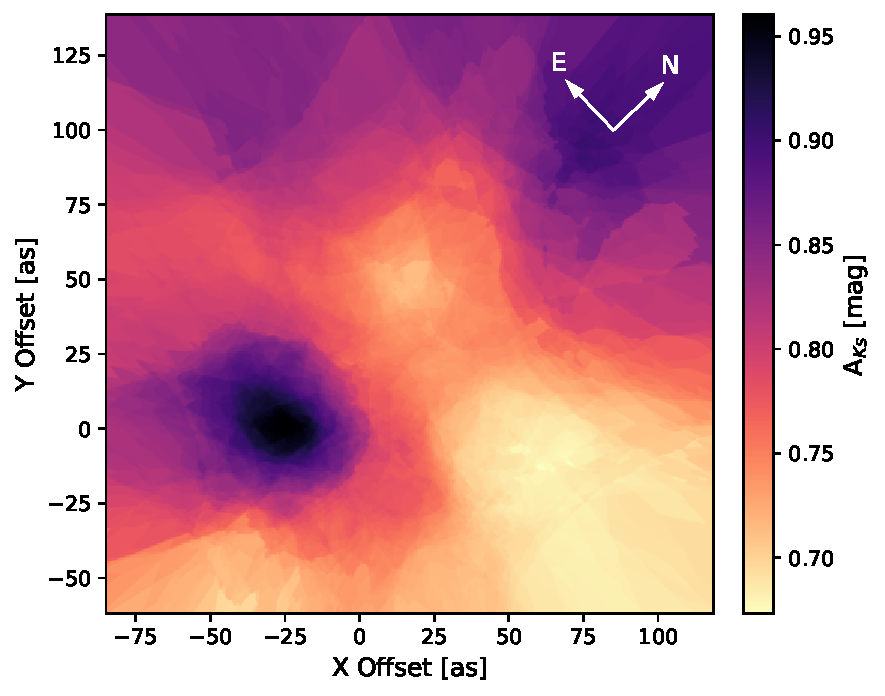
\includegraphics[width = 0.7\linewidth]{figures/chapter2/F125W_Redmap_w_ne.pdf}
\caption[Infrared extinction map of Westerlund 1]{IR extinction map produced by analysis of the extinction values of the MS stars. The map axes are referenced to the non-completeness corrected centroid of the cluster, weighted by the dereddened $\mathrm{F160W_D}$ magnitudes. The assigned pixel values are taken from the mean of the $30$-nearest $3\sigma$ clipped stars.}
\label{fig:wd1_red_map}
\end{figure} 


\begin{figure*}[htb!]
\centering
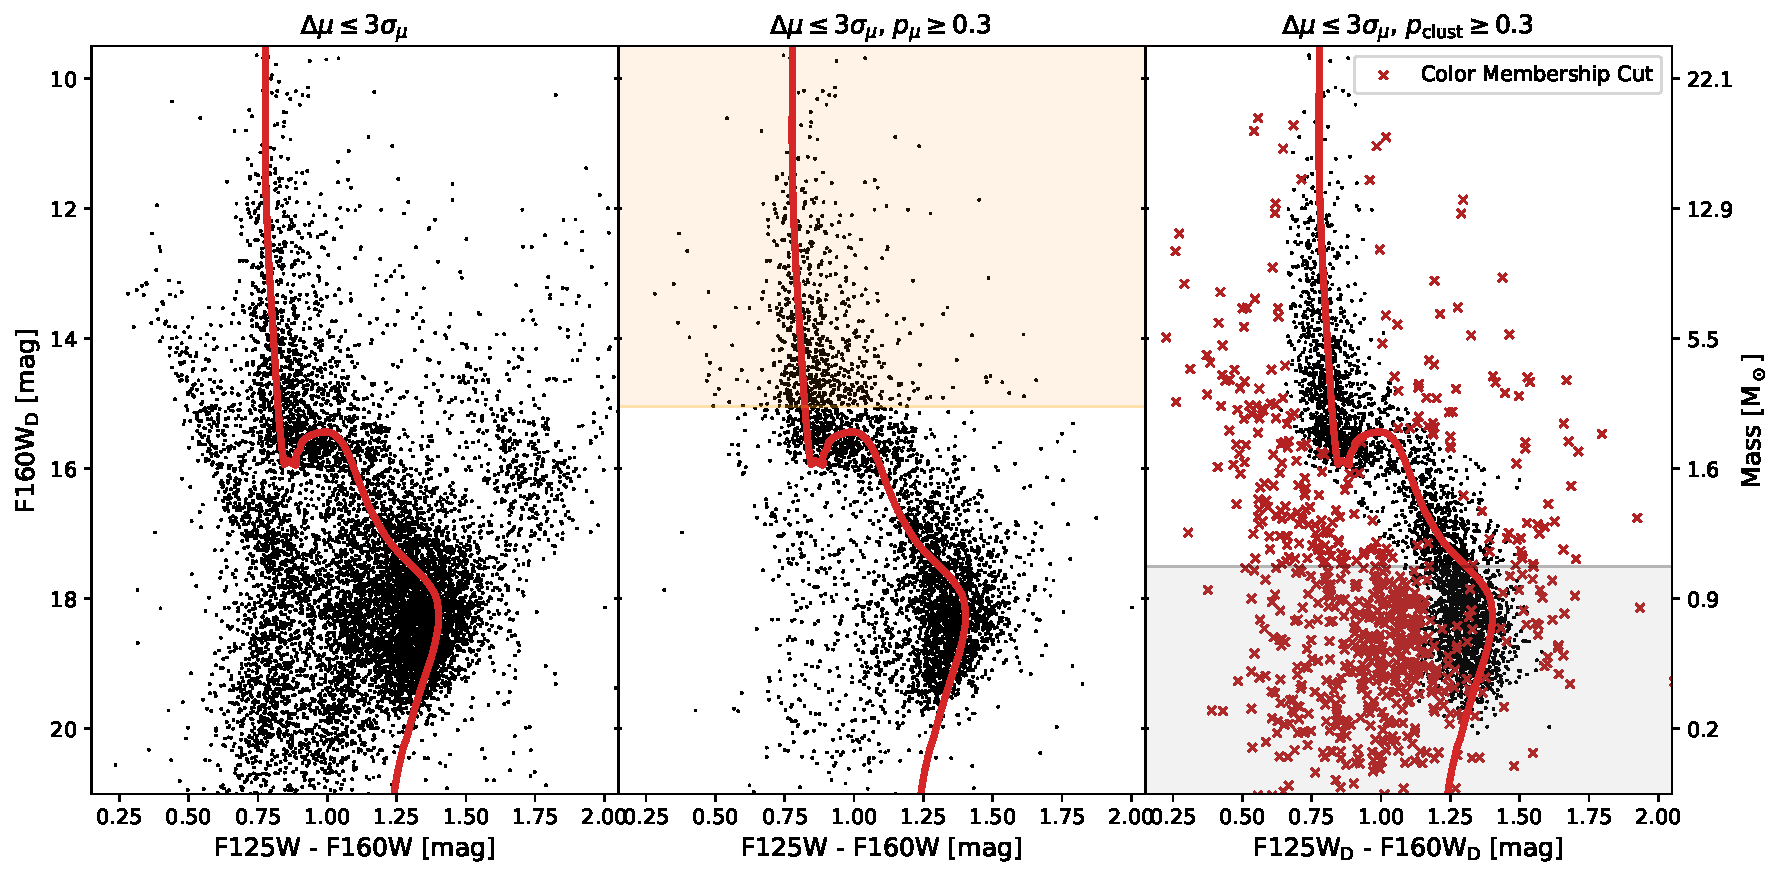
\includegraphics[width = \textwidth]{figures/chapter2/CMD_3_Panel.pdf}
\caption[Color-magnitude diagram of Westerlund 1]{{\em Left}: CMD of the cluster catalog after applying a $3\sigma_{\mu}$ box cut in the x and y directions. {\em Center}: CMD of cluster PM membership $p_\mu \geq 0.3$ and reference isochrone with an $\AKs$ of $0.73$~mags, distance of $4000$~pc and age of $7$~Myr. The {\em orange shaded} region indicates the faintest dereddened magnitude limit of $15.05$ $\mathrm{F160W_D}$ of the stars used to produce the extinction map. {\em Right}: CMD of cluster members with $\pclust \geq 0.3$ after extinction correction and color membership cut, with rejected stars marked with {\em red x's}. The {\em gray shaded} region corresponds to stars fainter than our completeness cut of $17.5$~mag.}
\label{fig:3_panel_population}
\end{figure*}


As the cluster is subject to known reddening \citep[][]{Negueruela-2022}, we correct for extinction by producing a spatial attenuation map and differentially deredden the stars in our sample. In the following analysis, we use the subscript D after the filter names to denote the dereddened magnitude. We create an extinction map for the field based on individual extinction values derived from high-probability main-sequence cluster members. The intrinsic colors of such stars are nearly independent of mass in the NIR filters. Therefore, their extinction can be estimated from their observed color, given an assumed distance and extinction law.

To determine the attenuation value $\AKs$, we used \texttt{spisea} \citep[][]{spisea} to produce a reference isochrone with a reference distance of $4000$~pc, age of $7$~Myr, and solar metallicity, which were adopted from literature values \citep[e.g.,][]{Beasor-2021, Navarete-2022} as described in Section~\ref{wd1-sec:introduction}. We emphasize that this is a reference isochrone used to calculate the extinction, as the MS stars used to derive the extinction values are insensitive to the cluster age and distance within a reasonable range. We will model the age and distance in Section~\ref{wd1-subsec:cmd_fitting} for mass assignment. The reference isochrone adopted a mixed set of stellar evolutionary models, including the Baraffe \citep[][]{Baraffe-2015}, Pisa \citep[][]{Tognelli-2011}, and the Geneva \citep[][]{Ekstrom-2012} models\footnote{\href{https://spisea.readthedocs.io/en/latest/evo_models.html\#evolution.MergedBaraffePisaEkstromParsec}{\texttt{spisea.evolution.MergedBaraffePisaEkstromParsec}}}. We then varied the cluster extinction $\AKs$ value using the revised extinction law of \citet{Hosek-2019}. This law has been derived using stars from the Arches and Wd1 for optical and near-infrared  (NIR) extinction in highly reddened regions. We adopted the isochrone with a reference $\AKs = 0.73$ for both the optical and NIR filters. We produced a secondary isochrone with the same attributes but with an attenuation of $\AKs = 1.03$, $0.3$ more than the reference isochrone, to calculate the slope of the shift of a star's position in the CMD, or the reddening vector, under a change in extinction.

We produced a pixel-by-pixel reddening map by utilizing high kinematic membership probability ($p_{\mathrm{clust}} \geq 0.7$) main-sequence (MS) stars brighter than $\mathrm{F160W} = 15.0$~mag, which is $0.5$~mag brighter than the PMS turn-on. We interpolate along mass in each isochrone and map reddening vectors as a function of mass between the fiducial and secondary isochrones. Each star is assigned an extinction value based on the distance from the reference isochrone along the nearest reddening vector.  We reject stars with $\AKs$ values further than $3$-$\sigma$ away from the mean $\AKs$, as well as stars with a distance further than $0.25$~mag from the nearest reddening vector on the CMD. After the rejection, we are left with $451$ stars out of $2934$ for assigning extinction values, with a median $\AKs = 0.79 \pm 0.06$~mag.

We assign each pixel an extinction value and error via the $3$-$\sigma$ clipped mean of the $30$ nearest neighbors among the $451$ stars used to calculate extinction. The resulting IR extinction map is shown in Figure~\ref{fig:wd1_red_map}. 
The extinction error map ($\sigma_{\mathrm{map}}$) is calculated as $\sigma_{\AKs}$ / $\sqrt{N}$, where $\sigma_{\AKs}$ is standard deviation of the extinction values and $N$ is the number of stars used. Stars in the catalog are assigned the extinction and error of the pixel they fall on. We build separate extinction maps from the optical and IR photometry to see which one results in a tighter cluster on the CMD.

In this work, we adopted the IR extinction map in F125W, shown in Figure~\ref{fig:wd1_red_map}. We noticed that the optical and IR extinction maps are remarkably consistent with the assumed extinction law. Both maps show significant spatial variability over a similar range of extinction values, with $\Delta\AKs = 0.29$~mag for both the optical and IR CMD-based maps. The median of both maps is $\AKs=0.79 \pm 0.06$~mags, with the error being the standard deviation of the map. The maps can differ by as much as $\vert\AKs\vert=0.03$~mag with a median absolute difference of $\AKs = 0.004$~mag. In addition, the median pixel value errors are both $\AKs = 0.013$~mag for the optical and IR CMD-based map. The maximum absolute difference between the pixel value errors of the two maps is $0.012$~mag. 

Our extinction maps are consistent with the observations of \citet{Brandner-2008}, in which the authors claimed that the regions east and north of the cluster center tend to have slightly higher extinctions, while the regions west and south of the cluster have slightly lower extinctions. \citet{Lim-2013} also found the east side of the field to have higher extinction than the west side, though they also observed the highest reddening towards the cluster center. In our extinction maps, a relatively high patch of reddening is found to the southeast of the uncorrected cluster center. The cause of this discrepancy is likely due to the smaller sample size of \citet{Lim-2013}, who measured the reddening of $53$ OB supergiants. Our reddening sample is much larger, allowing us to map out the differential reddening in more detail.

Figure~\ref{fig:3_panel_population} shows the CMDs before and after differentially dereddening the colors, along with the color membership cut. \textit{The magnitude limit of $\mathrm{F160W}_\mathrm{D} = 15.05$ mag for deriving the extinction map is shown as the orange shaded region in the middle panel. The red curves indicate the best-fit isochrone rather than the reference isochrone. The determination of the cluster's age and distance to generate the best-fit isochrone will be elaborated in Section~\ref{wd1-subsec:cmd_fitting}.}


\subsection{Completeness}
\label{wd1-subsec:completeness}

\begin{figure}[htb!]
    \centering
    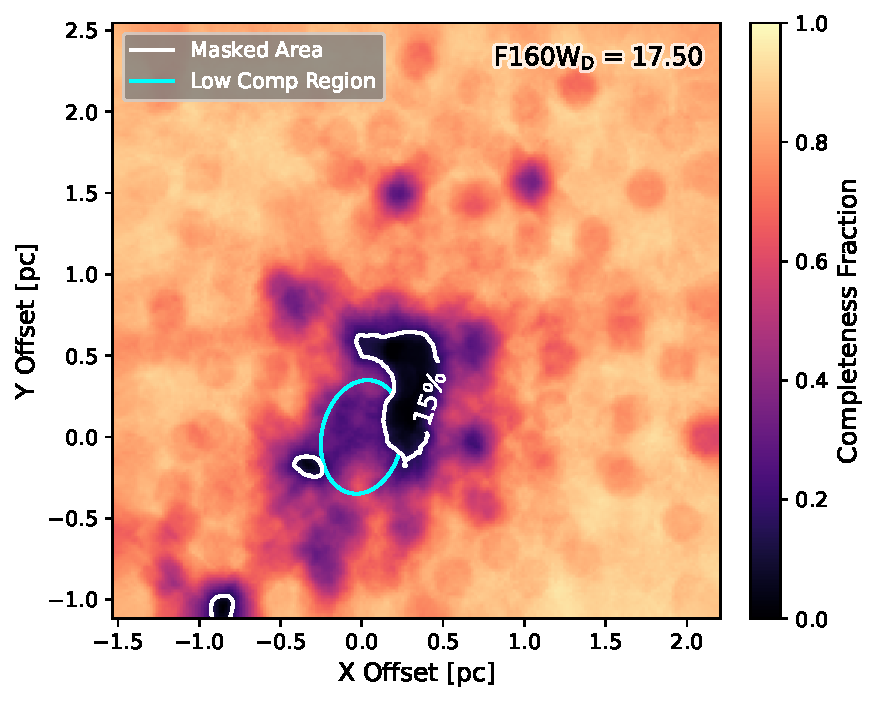
\includegraphics[width = 0.7\linewidth]{figures/chapter2/2D_completeness_F160W_0.15.pdf}
    \caption[Completeness map of Wd1]{2D completeness map for dereddened $\mathrm{F160W_D}$ mag of $17.5$. The white contours show the $15\%$ low completeness regions, which are masked in the radial profile analysis. The partial {\em cyan ellipse} shows the inner-most radial bin for completeness check with an effective radius of $0.29$~pc.}
    \label{fig:2D_completess}
\end{figure}

\begin{figure*}[htb!]
    \centering
    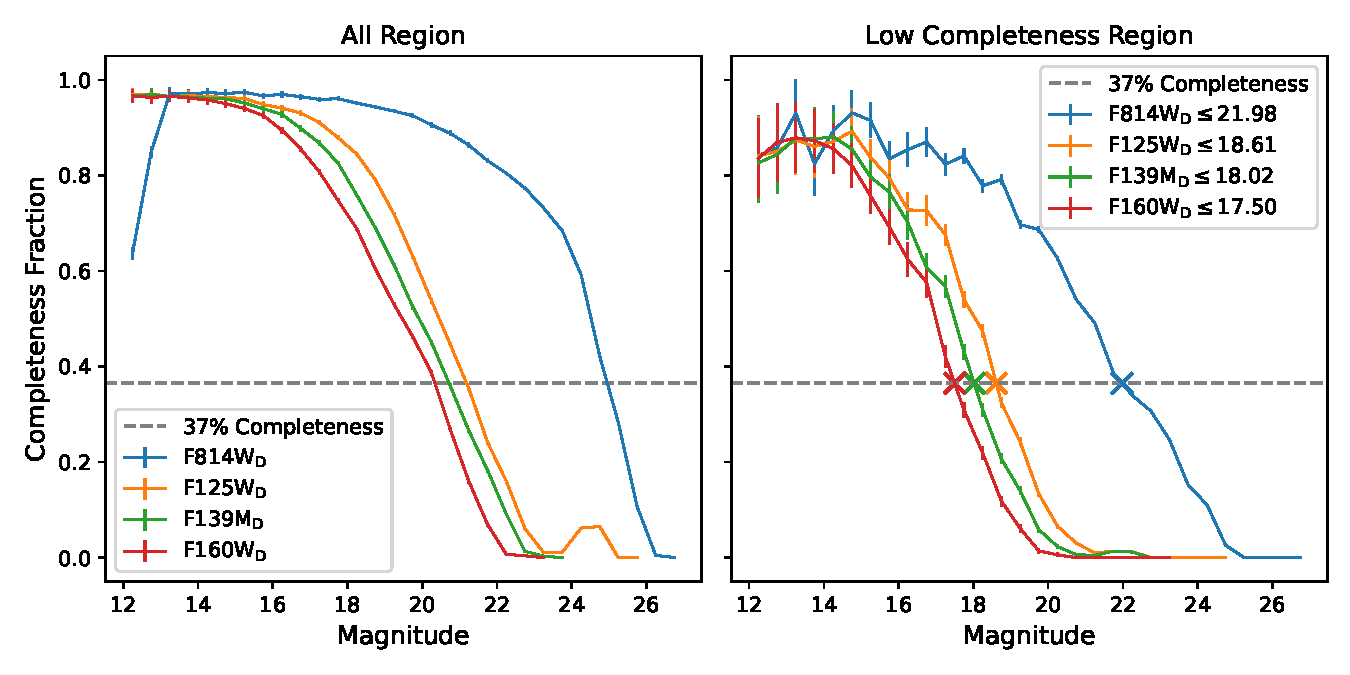
\includegraphics[width = \linewidth]{figures/chapter2/Completeness_Curves.pdf}
    \caption[Completeness vs. magnitude]{Completeness as a function of magnitude. {\em Left}: 1D completeness curves for the entire field. {\em Right}: 1D completeness curves for the low completeness region marked in Figure~\ref{fig:2D_completess}. The {\em gray dotted} line in each plot marks the $65\%$ completeness limit. After masking out the lowest $15\%$ completeness regions, our cut at $17.5$~mag in dereddened $\mathrm{F160W_D}$ is equivalent to a $65\%$ completeness limit in the low completeness region.}
    \label{fig:1D_comp_curves}
\end{figure*}

\begin{figure}[htb!]
    \centering
    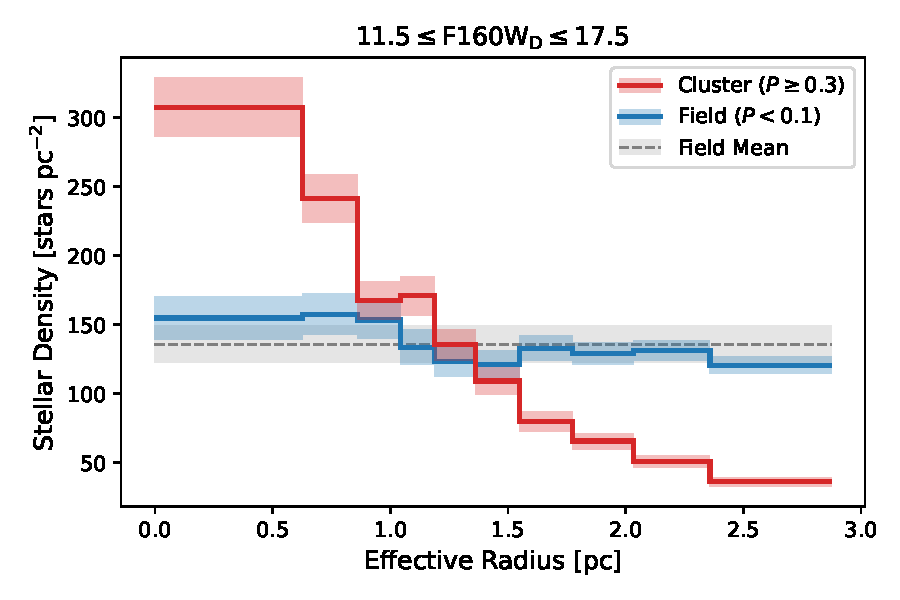
\includegraphics[width = 0.7\linewidth]{figures/chapter2/Field_Stellar_Density_11.5_17.5.pdf}
    \caption[Completeness-corrected cluster and field stellar density vs. effective radius]{Dependence of completeness-corrected cluster and field stellar densities on effective radius. Completeness is interpolated as a function of effective radius and magnitude. The cluster members with $\pclust \geq 0.3$ are shown in red, and the field stellar density with $\pclust < 0.1$ is shown in blue. The gray dashed line and shaded region represent the mean field stellar density across the effective radius.}
    \label{fig:field_density}
\end{figure}

As the region is crowded, completeness correction is vital to account for the unobserved stars contaminated by the bright stars. We estimate the completeness of our final catalog by planting a set of artificial stars into the original images and processing them through our entire analysis pipeline. The procedure for this analysis has been described in detail in earlier work \citep{Lu-2013, Hosek-2015, Hosek-2019, Rui-2019} and entails planting and extracting \num{600000} artificial stars. The positions of the artificial stars are randomly sampled from a uniform distribution over the FOV. The fluxes of the artificial stars are generated to thoroughly cover the color-magnitude space populated by the observed stars with some additional padding on all sides. 

We modify the astrometric and photometric errors of the detected artificial stars to incorporate additional systematic uncertainties, potentially arising from PSF variability, intra-pixel sensitivity variations, and uncorrected residual distortions in the simulations \citep{Hosek-2015}. The systematic error terms are then added in quadrature, ensuring that the resulting error distributions at different magnitudes for the simulated stars match those of the observed stars.

Artificial stars are matched across all filters and epochs, and their PMs are fit in the same manner as the observed data. After accounting for systematic errors in the observed stars, the final distribution of PM errors for the artificial stars matches the observed stars. There are \num{423790} out of \num{600000} stars detected in all four epochs: 2005 F814W, 2010 F160W, 2013 F160W and 2015 F160W. This catalog is used to construct a spatial completeness map and completeness curves as a function of magnitude.

To construct the completeness map, we first produce a grid of reference points of $1$~as-by-$1$~as in $x$ and $y$ directions. We determine the completeness of each reference point from its nearest \num{2000} neighbors in each filter and each magnitude bin ranging from $8$--$32$~mags with a step size of $0.5$~mag. Each reference pixel is assigned a completeness value for each magnitude bin. Observed stars are then assigned the completeness value of the nearest reference point. 

We masked the regions affected by low completeness smaller than $15\%$ at F160W$_\mathrm{D}=17.5$, or equivalently $1.12~M_\odot$, as shown in the white contours in Figure~\ref{fig:2D_completess}.  We tested the completeness correction in the unmasked FOV and in the lowest completeness region marked by the cyan ellipse with an effective radius of $0.35$~pc, ensuring the completeness levels are reasonable for the faintest magnitude. The size, orientation, and elongation of the ellipse are derived from the two-dimensional Gaussian profile fit to the stellar density map, which will be described in Section~\ref{wd1-subsec:density_modeling}. The effective radius accounts for the elongation and orientation of the cluster and will be defined in that Section.


To check the completeness correction, we first construct the 1D completeness curves by interpolating along the magnitudes for all of the remaining fields and the central low completeness region, respectively, as shown in Figure~\ref{fig:1D_comp_curves}. As can be seen from the completeness curves in the right panel in Figure~\ref{fig:1D_comp_curves}, cutting the stars fainter than F160W$_\mathrm{D}=17.5$ is equivalent to applying a $37\%$ completeness limit in the lowest completeness region.

Furthermore, we check the independence of the field stellar density on the effective radius, as is expected for a small FOV in our observation. For this purpose, we interpolate the completeness for each star only as a function of the effective radius and magnitude, instead of using the pixel completeness calculated as in Figure~\ref{fig:2D_completess}. Note that the interpolated completeness is only used to check the field stellar density, and the pixel completeness is used for the actual analysis. We use 2D interpolation on a magnitude grid ranging from $10$ to $22$~mag in $\mathrm{F160W_D}$ with a step size of $0.5$~mag, and on the $10$ radial bins which equally partition the corrected stellar count. The resulting cluster and field stellar densities as a function of effective radius after correcting for membership, completeness, and area fraction are shown in Figure~\ref{fig:field_density}. To confirm the independence of the field stellar density on effective radius after completeness correction, we performed a Kolmogorov--Smirnov (KS) test on \num{10000} simulated field stellar density arrays of length $10$, same as the length of radial bins in Figure~\ref{fig:field_density}, with each element following a normal distribution centered at the measured value and a standard deviation being the associated uncertainty in that bin. The simulated data is tested against a normal distribution with the expectation being the mean of the measured field stellar density across the effective radius, and the standard deviation being the standard deviation of $10$ measured field stellar densities. The null hypothesis is that the field stellar density in each bin follows the same Gaussian distribution, independent of the effective radius. The resulting $p$-value of the \num{10000} simulations is $0.50 \pm 0.27$, significantly greater than the critical value of $0.05$. Therefore, we accept the null hypothesis that the field stellar density is independent of effective radius, proving the validity of our completeness correction.



\subsection{Stellar Density Modeling}
\label{wd1-subsec:density_modeling}

Characterizing the stellar surface density and radial density profile of Wd1 requires accounting for both its known eccentricity \citep[e.g.,][]{Muno-2006, Brandner-2008, Gennaro-2011} and the edge effects introduced by the limited FOV. 

To quantify the elongation and orientation of the cluster, we fit a two-dimensional Gaussian profile to the stellar surface density map, using stars with $p_\mathrm{clust} \geq 0.3$ and $\mathrm{F160W_D}$ between $11.5$ and $17.5$~mag. Membership and completeness correction are incorporated in the surface stellar density by weighting each star with:
\begin{equation}
    w_i = \frac{\pmui}{C_i}\,,
    \label{eq:weight}
\end{equation}
with $p_\mu^i$ denoting the PM membership of the $i$-th star, and $C_i$ its completeness. The stellar density map is computed on a pixel grid. Specifically, the density at each pixel is calculated as the sum of the weights of the $50$ nearest stars from that pixel divided by the overlapping area between the masked image and a circle centered on the pixel, with its radius being the distance to the $50$th nearest neighbor.

Based on the best-fit Gaussian profile parameters, we define the effective radius:
\begin{equation}
    \reff = \sqrt{\left(\Delta x/\epsilon\right)^2 + \Delta y^2}\,,
    \label{eq:reff}
\end{equation}
where $\Delta x$ and $\Delta y$ are the offsets from the Gaussian center projected along the minor and major axes, respectively, and $\epsilon$ is the ratio of the minor to the major axis, or ellipticity. We note that the definitions of ellipticity and eccentricity vary in the literature. In this work, we adopt the eccentricity defined as $e = \sqrt{1 - \epsilon^2}$. The effective radius transforms stellar positions by scaling them along the minor axis to match the major axis of the Gaussian profile, thereby circularizing the spatial distribution and enabling radial analysis.

The limited FOV affects the accurate determination of the radial density profile. To account for the edge effect, we introduce the concept of area fraction $f(r_\mathrm{reff})$ as a function of the effective radius. The area fraction adjusts for the incomplete radial coverage near the edges. Specifically, consider an elliptical annulus with an effective radius of $\reff$ and a width of $d\reff$ oriented concentrically with the Gaussian surface density profile. The area fraction is defined as the ratio of the remaining area of the annulus within the completeness-masked image to the full area of the annulus, assuming an infinite FOV:
\begin{equation}
    f(\reff) = \frac{A_\mathrm{overlap}(\reff)}{A_\mathrm{total}(\reff)}\,,
    \label{eq:area_fraction}
\end{equation}
where $A_\mathrm{overlap}(\reff)$ is the remaining area and $A_\mathrm{total}(\reff)=2\pi\, \reff\,d\reff$ is the total area of the annulus, respectively. Despite the areas being calculated in the stretched coordinates with $\reff$, the ratio remains identical in the original coordinates. We interpolate the area fraction as a function of the effective radius for annuli with a width increment of $1$ pixel and concentric with the Gaussian profile.

Each star is then weighted by $w_i^{\reff}$ to determine the radial density profile:
\begin{equation}
    w_i^{\reff} = \frac{1}{f(\reff)}\frac{\pmui}{C_i}\,.
    \label{eq:radial_profile_weight}
\end{equation}
This weight is only used in radial profile modeling. To prevent amplifying the weights beyond reasonable levels, we cautiously restrict the area fraction $f(\reff) \geq 0.3$. 

Next, we fit the radial profile to an Elson, Fall, and Freeman model \citep[][EFF hereafter]{Elson-1987}, which has been found to be a good description of other young clusters \citep[][]{Mackey-2003a, Mackey-2003b, McLaughlin-2005, Rui-2019, Hosek-2015} as well as Wd1 \citep[][]{Gennaro-2011, Andersen-2017}. 
The EFF profile takes the form:
\begin{equation}
    \Sigma(\reff) = \Sigma_0 \left(1 + \frac{\reff^2}{a^2} \right)^{-\gamma / 2}
    \label{eq:radial_profile}
\end{equation}
where $\Sigma_0$ is the amplitude, $r$ is the radius, $a$ is the core parameter, and $\gamma$ is the slope of the power law. We assume our background contamination is zero, as the radial range explored in this work is insufficient to constrain the parameter robustly. The background contamination parameter is not constrained if included, and affects the convergence of other parameters due to degeneracies in the parameter space. The core parameter $a$ is related to the core radius $r_c$ of the cluster by:
\begin{equation}
    r_c = \frac{a}{\sqrt{2^{2/\gamma} - 1}}.
    \label{eq:rc}
\end{equation}
Note that we only model $r_c$, and the posterior of $a$ is purely converted from $r_c$ and shown for illustration purposes. 

To perform the EFF fit, we use \texttt{MultiNest} to maximize the log-likelihood function: 
\begin{equation}
    \log{\mathcal{L} = \sum_{i=1}^N w_i^{\reff} \log{\Sigma(\reff)}}
\end{equation}
where $N$ is the number of stars used for the fit, $w_i^{\reff}$ is the weight of each star defined in Equation~\eqref{eq:radial_profile_weight}, and $\Sigma(\reff)$ is the EFF model. We refer to \citet{Richardson-2011} and \citet{Cicuendez-2018} for the derivation and further discussion of the log-likelihood function and \citet{Do-2013} and \citet{Hosek-2015} for further discussion of the methodology.


\subsection{Color-Magnitude Diagram Fitting}
\label{wd1-subsec:cmd_fitting}
We performed a Bayesian approach identical to \citet{Hosek-2019} to model the cluster parameters in the CMD space using simulated synthetic clusters based on theoretical isochrones and infer the distance $d$ and age $t$ of the cluster. Here, we briefly summarize the modeling process and direct the readers to \citet{Hosek-2019} for further details. We used \texttt{spisea} \citep[][]{spisea} to generate the simulated model cluster with combined stellar evolutionary models, atmosphere models, a two-segment broken power law IMF, and an initial-final mass relation. The IMF has a slope of $\alpha_1$ for stellar mass below the break-point mass $m_\mathrm{break}$, and a slope of $\alpha_2$ for mass above $m_\mathrm{break}$. The free parameters include the cluster distance $d$, age $t$, average extinction value $AK_S$, differential extinction $dAK_S$, IMF break-point mass $m_\mathrm{break}$, higher-mass IMF slope $\alpha1$, the lower-to-higher mass IMF slope ratio $d\alpha=\alpha_2/\alpha_1$, break mass $m_\mathrm{break}$, and the cluster mass $M_\mathrm{cl}$. Specifically, stars were sampled from the IMF accounting for observationally unresolved multiplicity according to the parameters outlined in \citet{Lu-2013}, with a total mass of $M_\mathrm{sim} = 5\times10^6~M_\odot$ to reduce stochastic variations. The stellar physical properties were determined using the merged set of stellar evolutionary models in \texttt{spisea} as described in Section~\ref{wd1-subsec:extinction}. The derived stellar parameters were subsequently used as inputs for a set of stellar atmospheric models\footnote{\href{https://spisea.readthedocs.io/en/latest/atmo_models.html\#atmospheres.get\_merged\_atmosphere}{\texttt{spisea.atmospheres.get\_merged\_atmosphere}}}, and synthetic photometry of the stars was subsequently computed by \texttt{pysynphot} \citep[][]{pysynphot}. Each star in the simulated cluster was assigned a radius following the same distribution as the observed effective radius $\reff$ in Wd1.

The posterior probability function of the cluster parameters is given by the Bayesian theorem:
\begin{equation}
    \mathcal{L}\left(\theta\right) = p\left(\mathbf{k}, N|\theta\right) \cdot p\left(\theta\right),
    \label{eq:cmd_likelihood}
\end{equation}
where $\mathbf{k} = \lbrace\left(m_i, c_{1,i}, c_{2,i}\right)\rbrace_{i=1}^N$ denotes the CMD positions of $N$ observed stars in $\mathrm{F160W_D}$ magnitudes, $\mathrm{F814W_D} - \mathrm{F125W_D}$ color, and $\mathrm{F125W_D} - \mathrm{F160W_D}$ color, respectively. $p\left(\theta\right)$ is the prior function on the model parameters. The model parameter vector $\theta$ includes the cluster distance $d$, age $t$, extinction $\AKs$, differential extinction $\Delta\AKs$, total cluster mass $M_\mathrm{cl}$, as well as the break mass and slopes of the IMF. The likelihood function $p\left(\mathbf{k}, N|\theta\right)$ consists of two components:
\begin{equation}
    p\left(\mathbf{k}, N|\theta\right) = p\left(\mathbf{k}|\theta\right) \cdot p\left(N|\theta\right),
\end{equation}
where $p\left(\mathbf{k}|\theta\right)$ is the probability of the observed CMD given the model, and $p\left(N|\theta\right)$ is the Poisson probability of observing $N$ stars given the expected number of stars $N_\mathrm{exp}$ of the model. The CMD likelihood is calculated as the product of the CMD probability of each star:
\begin{equation}
    p\left(\mathbf{k} | \theta\right) = \prod_{i=1}^n p\left(\mathbf{k}_i | \theta\right).
\end{equation}
For each star, we modeled its CMD probability as a multivariate normal distribution centered at the observed values with the standard deviation being the uncertainties $\mathcal{N}\left(\mathbf{k}_i, \mathbf{\sigma}_i\right)$. The individual stellar CMD likelihood is then calculated as the normal distribution convolved with a mixture of cluster and field model cluster CMD probability density function (PDF) weighted by the corresponding membership probability:
\begin{align}
    p\left(\mathbf{k}_i | \theta\right) 
    &= \int \mathcal{N} \left(\mathbf{k} ; \mathbf{k}_i, \mathbf{\sigma}_i\right) \bigg[
        p_\mu \cdot f_\mathrm{cl}\left( \mathbf{k}_\mathrm{sim} | \theta\right) \nonumber \\
    &\quad + \left(1 - p_\mu\right) \cdot f_\mathrm{field}\left( \mathbf{k}_\mathrm{field} \right)
    \bigg] \, d\mathbf{k},
\end{align}
where $\mathcal{N} \left(\mathbf{k}; \mathbf{k}_i, \mathbf{\sigma}_i\right)$ denotes the PDF of multivariate normal distribution with mean of $\mathbf{k}_i$ and standard deviation of $\mathbf{\sigma}_i$, $p_\mu$ is the PM membership probability, $f_\mathrm{cl}\left( \mathbf{k}_\mathrm{sim}| \theta \right)$ is the CMD PDF weighted by the completeness as a function of effective radius $C\left(\reff\right)$, and $f_\mathrm{field}$ is the CMD PDF of the field contamination population.

The total number likelihood is given by:
\begin{equation}
    p\left(N|\theta\right) = \frac{\left(N_\mathrm{exp}\right)^N \exp\left(-N_\mathrm{exp}\right)}{N!},
\end{equation}
where $N$ is the number of observed stars, and $N_\mathrm{exp}$ is the number of expected stars given $\theta$. The expected number of stars is determined by linearly scaling the completeness-corrected number of stars in the simulated cluster by the ratio of the observed cluster mass to the simulated cluster mass:
\begin{equation}
    N_\mathrm{exp} = N \times \frac{M_\mathrm{cl}}{M_\mathrm{sim}}\,.
\end{equation}

With the likelihood function, we used the \texttt{emcee} to sample the posterior distribution of the model parameters with $100$ walkers, $300$ steps, and the \texttt{KDEMove}. The results are presented in Section~\ref{wd1-subsec:age_distance}.


\section{Results}
\label{wd1-sec:results}
We present the full cluster catalog with PMs, dereddened magnitudes, kinematic and color membership probabilities, and completeness values of each star in Table~\ref{wd1-tab:results}. In this section, we use the catalog to model and analyze the properties of Wd1, including its surface density, morphology, radial density profile, age, distance, velocity dispersion, and mass segregation.


\begin{deluxetable}{lcccrrrrcccccccr}
\rotate
\tablewidth{0pt}
\tabletypesize{\scriptsize}
\tablecaption{Photometric, Kinematic, and Structural Properties of Wd1}
\tablehead{
    \colhead{ID} & 
    \colhead{$\mathrm{F814W_D}$} & 
    \colhead{$\mathrm{F125W_D}$} & 
    \colhead{$\mathrm{F160W_D}$} & 
    \colhead{$\Delta\alpha_0$\tablenotemark{a}} & 
    \colhead{$\Delta\delta_0$} & 
    \colhead{$\mu_{\alpha^*}$} &
    \colhead{$\mu_\delta$} & 
    \colhead{$t_0$} & 
    \colhead{$p_\mu$} & 
    \colhead{$p_\mathrm{color}$} & 
    \colhead{$\pclust$} & 
    \colhead{$C$} & 
    \colhead{$M$} & 
    \colhead{$\reff$} & 
    \colhead{$f(\reff)$}
    \\
    \colhead{---} & 
    \colhead{mag} & 
    \colhead{mag} & 
    \colhead{mag} & 
    \colhead{$\arcsec$} & 
    \colhead{$\arcsec$} & 
    \colhead{$\rm mas\,yr^{-1}$} &
    \colhead{$\rm mas\,yr^{-1}$} & 
    \colhead{yr} & 
    \colhead{---} & 
    \colhead{---} & 
    \colhead{---} & 
    \colhead{---} & 
    \colhead{$M_\odot$} & 
    \colhead{pc} & 
    \colhead{---}
}
\startdata
wd1 00001 & $18.50$ & $15.17$ & $14.29$ & $-29.13$ & $-17.96$ & $-0.49 \pm 0.14$ & $-0.19 \pm 0.15$ & $2011.698$ & $0.30$ & $1$ & $0.30$ & $0.97 \pm 0.21$ & $4.86$ & $0.67$ & $0.87$ \\
wd1 00002 & $18.88$ & $15.41$ & $14.50$ & $-53.11$ & $66.75$ & $0.53 \pm 0.04$ & $0.35 \pm 0.04$ & $2010.997$ & $0.59$ & $1$ & $0.59$ & $0.97 \pm 0.18$ & $4.40$ & $2.15$ & $0.61$ \\
wd1 00003 & $17.54$ & $14.57$ & $13.83$ & $3.09$ & $149.75$ & $-0.01 \pm 0.05$ & $0.21 \pm 0.04$ & $2009.482$ & $0.89$ & $1$ & $0.89$ & $1.00 \pm 0.19$ & $5.99$ & $3.11$ & $0.18$ \\
wd1 00004 & $18.51$ & $15.28$ & $14.45$ & $98.79$ & $26.37$ & $0.06 \pm 0.02$ & $0.10 \pm 0.02$ & $2008.278$ & $0.92$ & $1$ & $0.92$ & $0.99 \pm 0.18$ & $4.51$ & $2.20$ & $0.58$ \\
wd1 00005 & $19.50$ & $15.80$ & $14.84$ & $40.85$ & $61.87$ & $0.10 \pm 0.04$ & $0.25 \pm 0.04$ & $2009.879$ & $0.90$ & $1$ & $0.90$ & $0.96 \pm 0.16$ & $3.74$ & $1.34$ & $0.82$ \\
\nodata & \nodata & \nodata & \nodata & \nodata & \nodata & \nodata & \nodata & \nodata & \nodata & \nodata & \nodata & \nodata & \nodata \\
\enddata
\tablecomments{Description of columns: \textit{ID}: Star name. \textit{$\mathrm{F814W_D}$, $\mathrm{F125W_D}$, $\mathrm{F160W_D}$}: mags in corresponding filters (Vega). \textit{$\Delta\alpha_0^*$, $\Delta\delta_0$}: Relative position in RA and DEC at time $t_0$. \textit{$t_0$}: Average observation time weighted by the inverse of astrometric uncertainties. \textit{$p_\mu$}: Proper motion membership. \textit{$p_\mathrm{color}$}: Color membership. \textit{$p_\mathrm{clust}$}: Product of proper motion membership and color membership. \textit{$C$}: Completeness. \textit{$M$}: Stellar mass. \textit{$\reff$}: Effective radius. \textit{$f(\reff)$}: Area fraction.
\tablenotetext{a}{Positions are relative to $\mathrm{RA}=16^{\textnormal{h}} 47^{\textnormal{m}} 04.0^{\textnormal{s}}$, $\mathrm{DEC}=\ang{-45} 51\arcmin 04.7\arcsec$ (J2000).}
(This table is available in its entirety in machine-readable form.)
}
\label{wd1-tab:results}
\end{deluxetable}



\subsection{Surface Density and Morphology}
\label{wd1-subsec:surface_density}
\normalcolor
\begin{figure}[htb!]
    \centering
    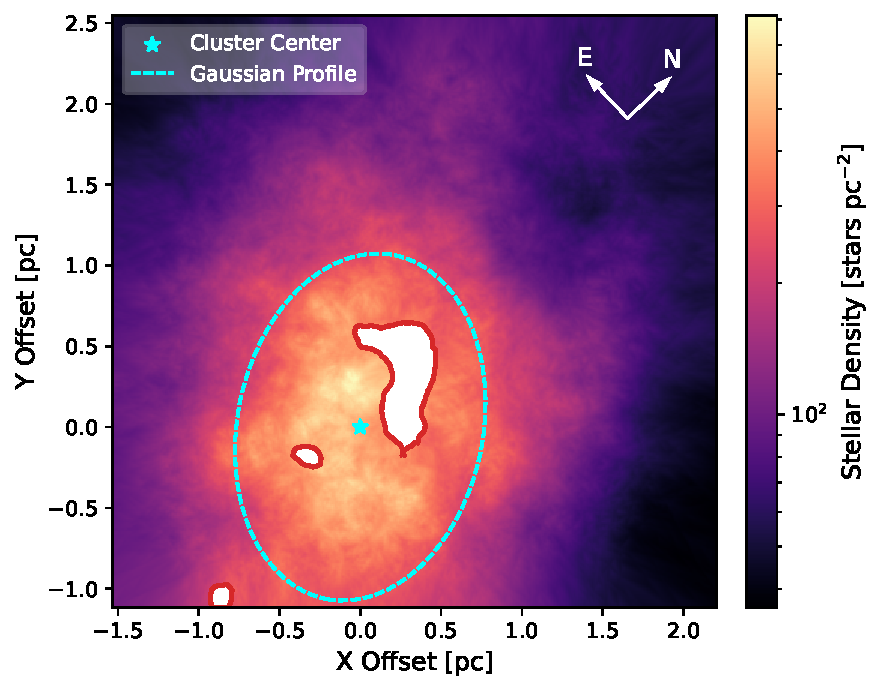
\includegraphics[width = 0.7\linewidth]{figures/chapter2/2D_Density_Map_w_ne_log.pdf}
    \caption[Stellar density map corrected by membership probability and completeness]{Stellar density map corrected by membership probability and completeness for stars with $\pclust \geq 0.3$ and $\mathrm{F160W_D}$ between $11.5$ and $17.5$~mag. The cyan star and dashed ellipse indicate the cluster center and the best-fit Gaussian profile, respectively. Note that the centroid has shifted to the lower left, or south. This is due to the large extinction values in that area being accounted for in this map.}
    \label{fig:2D_density_map}
\end{figure}

\begin{figure*}[htb!]
    \centering
    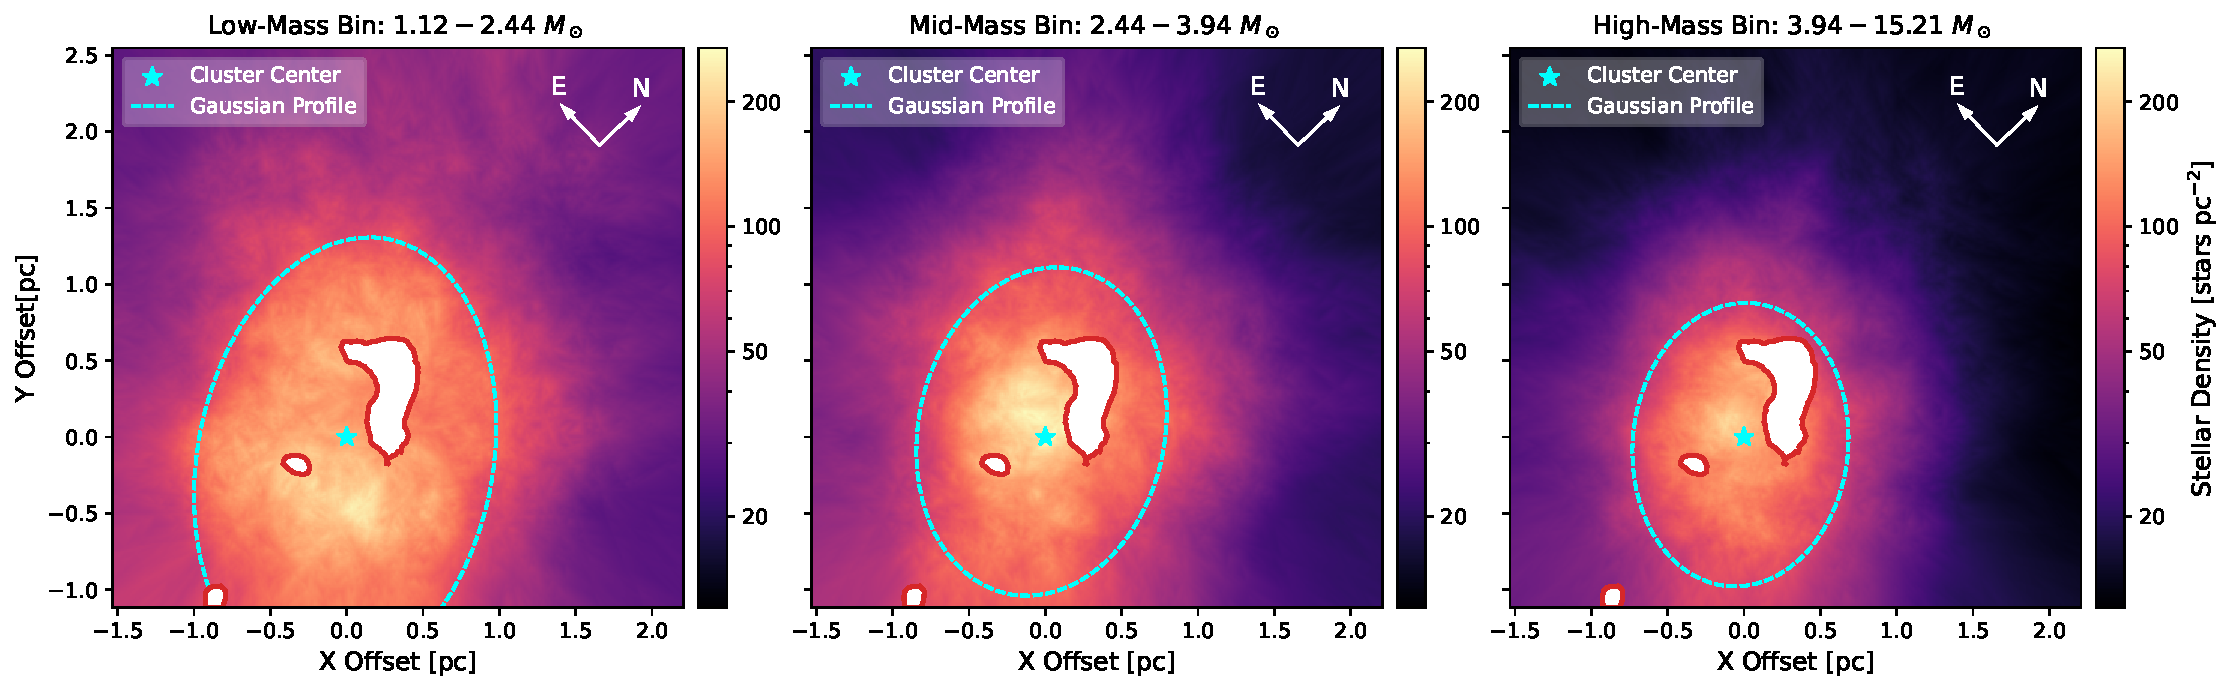
\includegraphics[width = \linewidth]{figures/chapter2/3_panel_density_check_plot_log.pdf}
    \caption[Stellar density map for increasing mass bins]{Stellar density map for increasing mass bins. The cyan star marks the center of the full cluster, and the dashed ellipse shows the Gaussian profile for each individual mass bin. Note that the colormap used in each panel is in log-scale and consistent.}
    \label{fig:binned_density}
\end{figure*}
We calculate the surface stellar density map of stars with $p_\mathrm{clust} \geq 0.3$ and $\mathrm{F160W_D}$ between $11.5$ and $17.5$~mag with membership and completeness correction. This results in a star count of $N = 1951$. 

To determine the morphology of Wd1, including its orientation, centroid, and elongation, we fit a 2D Gaussian profile to the membership and completeness-corrected stellar density map as described in Section~\ref{wd1-subsec:density_modeling}. Throughout this work, we adopted the center of the Gaussian density profile as the Wd1 center, located at $\mathrm{RA}=16^{\textnormal{h}} 47^{\textnormal{m}} 04.0^{\textnormal{s}}$, $\mathrm{DEC}=\ang{-45} 51\arcmin 04.7\arcsec$ (J2000). We find that the cluster is elongated in a northeast-southwest direction, with the major axis at a position angle of $\sim$\ang{35.2} 
east of north. This aligns the elongation with the Galactic plane and cluster PM movement spread, as seen in Figure~\ref{fig:wd1_vpd_distribution}. The flattening or ellipticity of the Gaussian profile $\epsilon$, defined as the ratio of the minor to the major axis, is approximately $0.70$, translating to an eccentricity of $e = \sqrt{1 - \epsilon^2} = 0.71$. 

The stellar density map and the Gaussian profile of the full catalog and three mass bins are shown in Figure~\ref{fig:2D_density_map} and Figure~\ref{fig:binned_density}, respectively. The cyan star represents the cluster center, and the dashed ellipse marks the $1$--$\sigma$ contour of the 2D Gaussian density profile. Both figures adopt the log-scale colormap. The elongation and its direction can be observed from Figure~\ref{fig:2D_density_map}. The decrease in size with increasing mass is clearly visible in Figure~\ref{fig:binned_density} under an identical colormap for each mass bin, indicating that the massive stars are more concentrated in the center.


\subsection{Radial Density Profile}
\label{wd1-subsec:radial_profile}

\begin{figure*}[htb!]
\centering
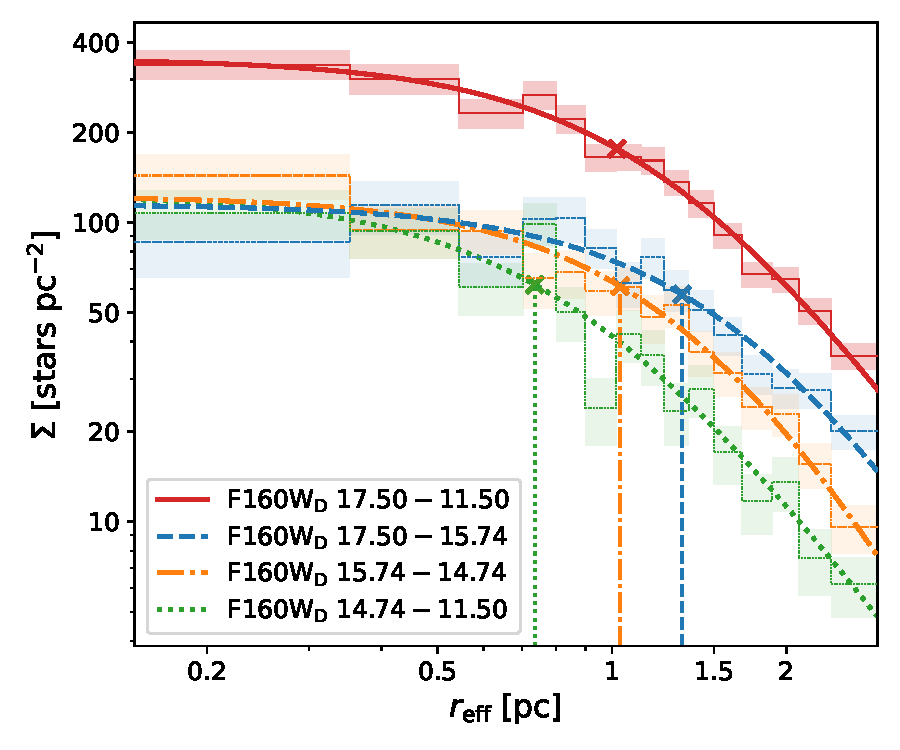
\includegraphics[width = 0.496\linewidth]{figures/chapter2/Radial_Profile.pdf}
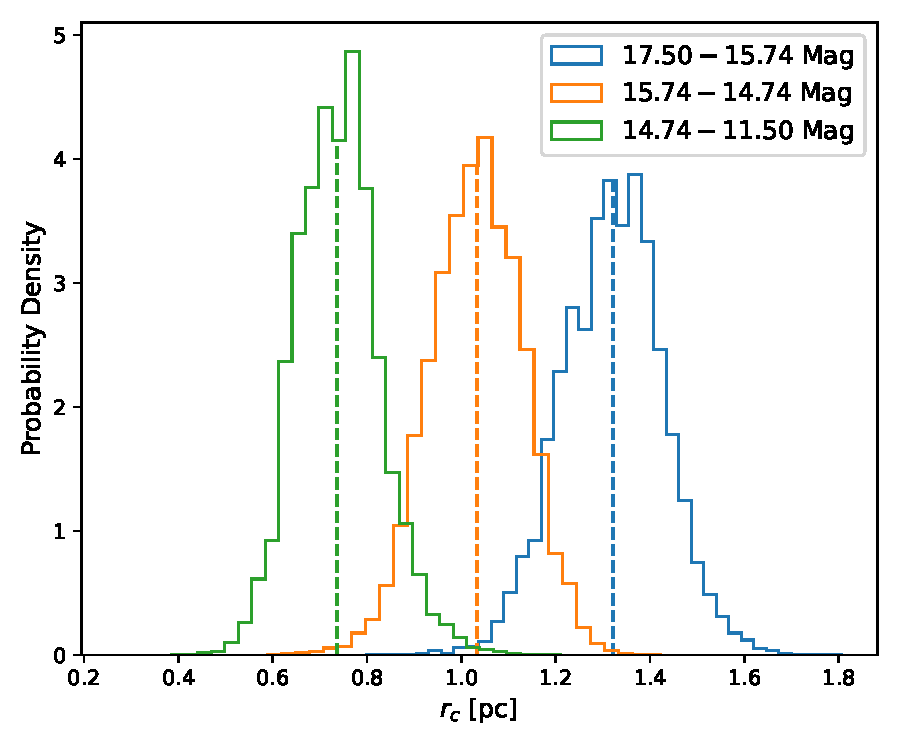
\includegraphics[width = 0.496\linewidth]{figures/chapter2/rc_distributions.pdf}
\caption[Binned radial profile and EFF model in each mass bin]{{\em Left}: Binned radial profile and EFF model in each mass bin. The binned radial profile is represented as the stair plots, and the EFF model is shown as the curves. The width of each stair corresponds to the bin $\reff$ range, and the shaded region represents the Poisson uncertainty. Bins were chosen to have an equal number of stars weighted by $w_i^r$ with the area fraction $f \geq 0.30$, which corresponds to $\reff \leq 2.87$~pc. {\em Right}: Posterior distributions of $r_c$ with the median value marked with a dashed line.}
\label{fig:mass_binned_radial_profile}
\end{figure*}

\begin{figure*}[htb!]
    \centering
    \gridline{
        \fig{figures/chapter2/EFF_posteriors_full_catalog.pdf}{0.491\linewidth}{(a) Full catalog}
        \fig{figures/chapter2/EFF_posteriors_low_mass_bin.pdf}{0.491\linewidth}{(b) Low-mass bin}
    }
    \gridline{
        \fig{figures/chapter2/EFF_posteriors_mid_mass_bin.pdf}{0.491\linewidth}{(c) Mid-mass bin}
        \fig{figures/chapter2/EFF_posteriors_high_mass_bin.pdf}{0.491\linewidth}{(d) High-mass bin}
    }
    \caption[Radial profile posteriors]{Weighted posterior distributions of EFF radial profile parameters. (a): Full catalog. (b): Low-mass bin. (c): Mid-mass bin. (d): High-mass bin. The red lines mark the weighted median, and the gray dashed line marks the weighted $16$- and $84$-th percentiles. Note that we only modeled $r_c$, and the posterior distribution of $a$ is purely converted from $r_c$.}
    \label{fig:radial_profile_posteriors}
\end{figure*}


We derive the best-fit models based on the entire catalog and divide the full sample into $3$ mass bins with a total weight ratio of roughly $4:3:2$ from the lowest to highest mass to explore the difference in radial density for each mass bin. 

Together with the completeness magnitude cut at F160$_\mathrm{D} \leq 17.50$, or equivalently $M \geq 1.12 M_\odot$ under the best-fit isochrone to be discussed in Section~\ref{wd1-subsec:age_distance}, we ended up with a maximum effective radius of $2.87$~pc. The resulting catalog has \num{1887} uncorrected stars, or $2304.6$ stars after being weighted by Equation~\eqref{eq:radial_profile_weight}. 

Figure~\ref{fig:mass_binned_radial_profile} shows the best-fit EFF model and the measured radial profiles in $15$ radial bins that share the same center, orientation, and elongation with the Gaussian density profile and contains an equal number of weighted sources. It is worth mentioning that the observed values represented as the stair plot in Figure~\ref{fig:mass_binned_radial_profile} are calculated as the sum of weights defined in Equation~\eqref{eq:radial_profile_weight} divided by the actual area of each bin, which allows a more accurate representation of density in each bin. The area fraction-corrected weight in Equation~\eqref{eq:radial_profile_weight} is only used in EFF profile modeling. The posteriors of the EFF radial profile fits are shown in Figure~\ref{fig:radial_profile_posteriors} for the full and $3$ binned catalogs. The aforementioned low completeness region in Figure~\ref{fig:2D_completess} is the innermost radial bin. 


The results of the EFF profile model parameters are summarized in Table~\ref{wd1-tab:eff_fit}, including the comparison with the Arches and Quintuplet cluster that will be discussed in Section~\ref{wd1-subsec:arches_quint}. The core radius $r_c$ of the full cluster is $0.10^{+0.07}_{-0.06}$ pc, and it decreases with increasing mass, indicating mass segregation: higher mass stars tend to be more concentrated in the center.

{\setlength{\tabcolsep}{5pt}  % Default is 6pt
\begin{deluxetable*}{lccr}
\tablecaption{Cluster Sample Size by Criteria}
\label{wd1-tab:cluster_statistics}
\tablewidth{0pt}
\tabletypesize{\scriptsize}
\tablehead{
\colhead{Catalog} &
\colhead{Cut Type} &
\colhead{Observed Stars\tablenotemark} & 
\colhead{Weighted Stars\tablenotemark{a}}
}% taken from /u/lwei/Westerlund1/Structure_Analysis/Structure/New_IMF_Fit/g_u/Bin_P_0.3/F160W_Mass_1.00_12.14/Elson_Fit/wd1_elson_fit.log
\startdata
Proper Motions & Detection in all Years & \num{10346} & --- \\
Proper Motion Box Cut & $v_x, v_y < 3\sigma_{pm}$ & \num{10002} & --- \\
Kinematic Probability Cut & $p_\mu \geq 0.3$ & $4341$ & --- \\
Kinematic and Color Cut & $\pclust \geq 0.3$ & $3582$ & --- \\
Radial Profile, Full Cluster & $17.50 \geq \mathrm{F160W}_\mathrm{D} \geq 11.50$, $\reff \leq 2.87$~pc & $1887$ & $2304.6$ \\
Radial Profile, Low-Mass Bin & $17.50 \geq \mathrm{F160W}_\mathrm{D} \geq 15.74$ & $762$ & $1024.6$ \\
Radial Profile, Mid-Mass Bin & $15.74 \geq \mathrm{F160W}_\mathrm{D} \geq 14.74$ & $627$ & $767.6$ \\
Radial Profile, High-Mass Bin & $14.74 \geq \mathrm{F160W}_\mathrm{D} \geq 11.50$ & $498$ & $512.4$ \\
Radial Profile, Arches Comparison & $4.50~M_\odot \leq M \leq 15.21~M_\odot$ & $396$ & $394.2$ \\
Radial Profile, Quintuplet Comparison & $2.50~M_\odot \leq M \leq 15.21~M_\odot$ & $1074$ & $1210.2$ \\
\enddata
\tablenotetext{a}{The weight refers to $w_i^{\reff}$ in Equation~\eqref{eq:radial_profile_weight} and requires the completeness and area fraction, which is not yet calculated for the first four rows.}
\end{deluxetable*}}


\begin{deluxetable*}{lccccccc}
\tablecaption{EFF Radial Profile Results}
\label{wd1-tab:eff_fit}
\tablewidth{0pt}
\tabletypesize{\scriptsize}

\tablehead{
\colhead{Sample} &
\colhead{$M$} &
\colhead{$\mathrm{F160W_D}$} &
\colhead{$\reff$\tablenotemark{a}} &
\colhead{$\gamma$\tablenotemark{b}} &
\colhead{$r_c$\tablenotemark{c}} &
\colhead{$a$} &
\colhead{$\Sigma_0$}\\
\colhead{---} & 
\colhead{M$_\odot$} & 
\colhead{mag} & 
\colhead{pc} & 
\colhead{---} & 
\colhead{pc} & 
\colhead{pc} & 
\colhead{stars pc$^{-2}$}
}
\startdata
Full Cluster & $1.12$--$15.21$ & $17.50$--$11.50$ & $\leq 2.87$ & $2.85^{+0.41}_{-0.35}$ & $1.02 \pm 0.06$ & $1.29^{+0.19}_{-0.17}$ & $352.05^{+20.94}_{-19.59}$ \\[0.5em]
Low-Mass Bin & $1.12$--$2.25$ & $17.50$--$15.74$ & $\leq 2.87$ & $3.31^{+1.30}_{-0.77}$ & $1.32^{+0.10}_{-0.11}$ & $1.84^{+0.54}_{-0.41}$ & $114.93^{+9.13}_{-7.71}$ \\[0.5em]
Mid-Mass Bin & $2.25$--$3.94$ & $15.74$--$14.74$ & $\leq 2.87$ & $3.63^{+1.18}_{-0.77}$ & $1.03 \pm 0.10$ & $1.52^{+0.42}_{-0.33}$ & $122.34^{+13.06}_{-10.64}$ \\[0.5em]
High-Mass Bin & $3.94$--$15.21$ & $14.74$--$11.50$ & $\leq 2.87$ & $2.67^{+0.50}_{-0.38}$ & $0.74 \pm 0.08$ & $0.89^{+0.20}_{-0.17}$ & $123.78^{+16.94}_{-13.50}$ \\[0.5em]
Arches Comparison & $4.5$--$15.21$ & $14.45$--$11.50$ & $\leq 2.87$ & $2.60^{+0.49}_{-0.36}$ & $0.74^{+0.09}_{-0.10}$ & $0.87^{+0.21}_{-0.18}$ & $92.23^{+14.56}_{-11.62}$ \\[0.5em]
Quint Comparison & $2.5$--$15.21$ & $15.69$--$11.50$ & $\leq 2.87$ & $3.27^{+0.62}_{-0.49}$ & $0.99^{+0.07}_{-0.08}$ & $1.35^{+0.27}_{-0.21}$ & $193.39^{+16.51}_{-13.28}$
\enddata
\tablecomments{Description of columns. \textit{Sample}: Star sample used in corresponding analysis. \textit{$M$}: Mass range of each sample. \textit{$\mathrm{F160W_D}$}: Dereddened magnitude in F160W. \textit{$\reff$}: Effective radius as defined in Equation~\eqref{eq:reff}. \textit{$\gamma$}: Slope of the radial profile power law in Equation~\eqref{eq:radial_profile}. \textit{$r_c$}: Core radius in Equation~\eqref{eq:rc}. \textit{$a$}: Core parameter converted from $r_c$ and not sampled. \textit{$\Sigma_0$}: Amplitude of the radial profile in Equation~\eqref{eq:radial_profile}.}

\tablenotetext{a}{Radius limit set by the distance at which the area fraction $f \geq 0.3$.}
\tablenotetext{b}{Uniform prior \U{1}{6}.}
\tablenotetext{c}{Uniform prior \U{0}{2}}
\end{deluxetable*}


\subsection{Age and Distance}
\label{wd1-subsec:age_distance}

\begin{figure*}[htb!]
    \centering
    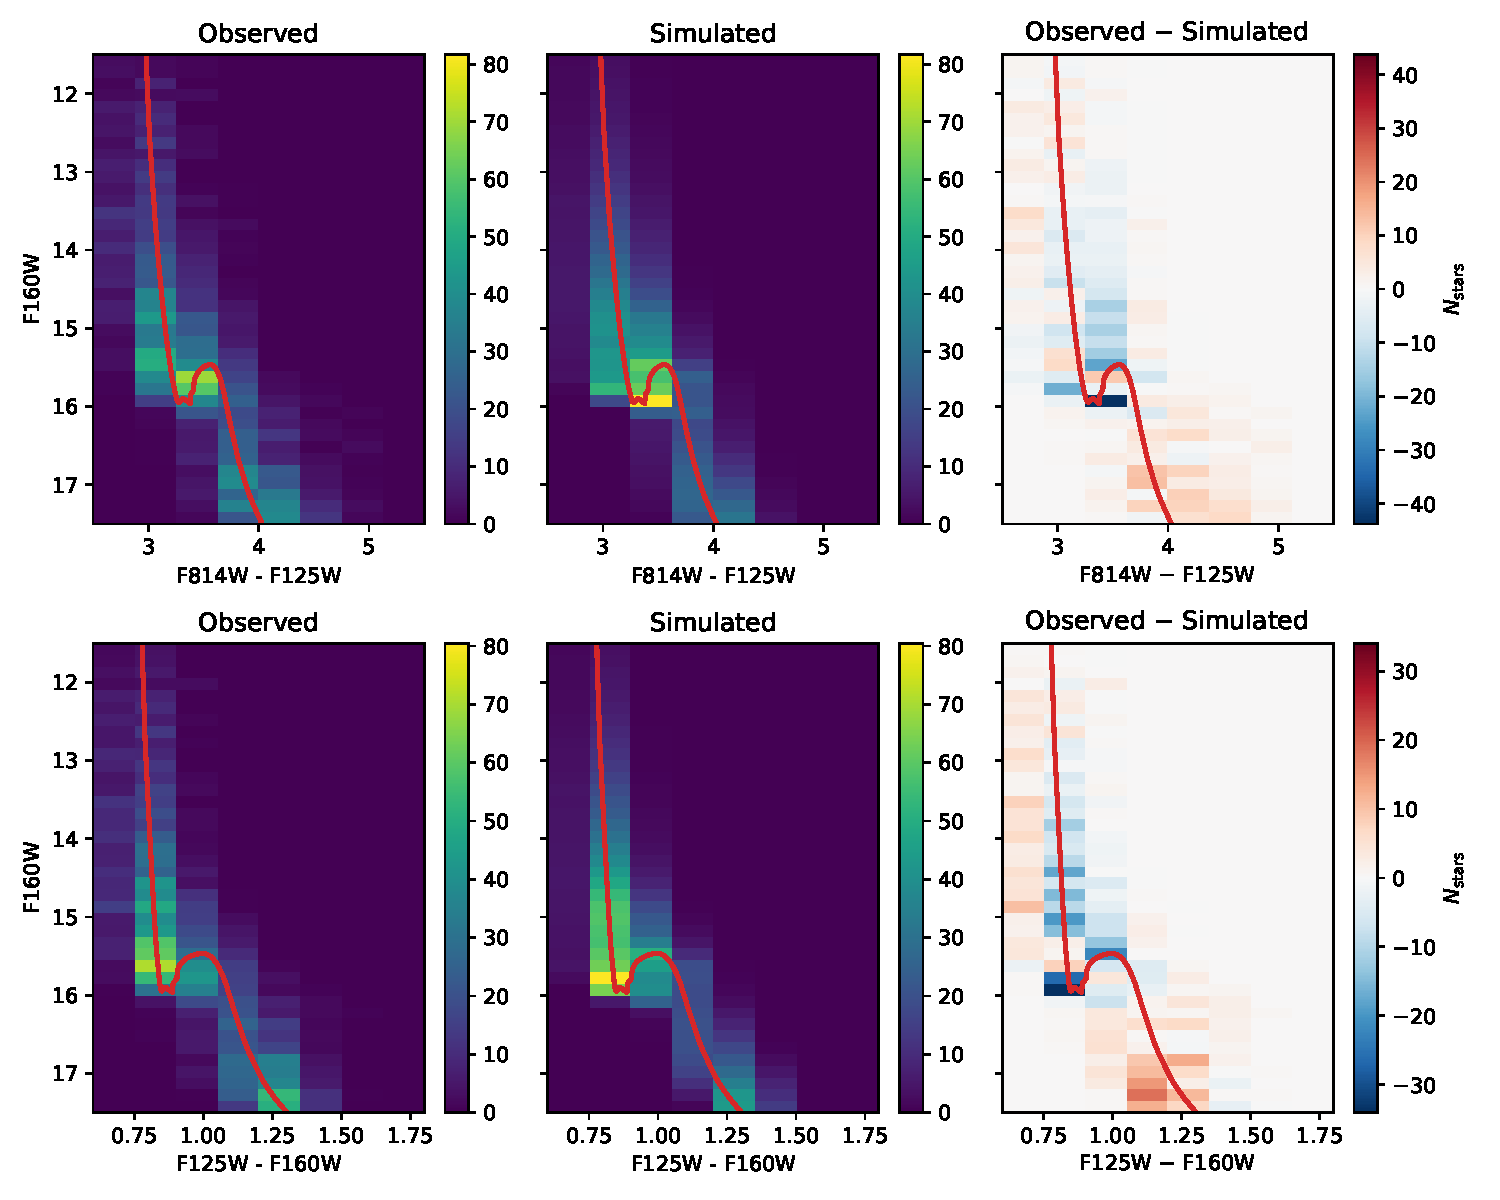
\includegraphics[width=\linewidth]{figures/chapter2/CMD.pdf}
    \caption[Observed and best-fit simulated cluster binned CMD and the residual.]{Observed and best-fit simulated cluster binned CMD and the residual. The top row shows the $\mathrm{F814W_D} - \mathrm{F125W_D}$ color and the bottom row shows the $\mathrm{F125W_D} - \mathrm{F160W_D}$ color. The left, middle, and right columns correspond to the observed CMD, simulated CMD, and the residual, respectively. The best-fit isochrone is overplotted as the red curve. The left and middle columns share the same colormap range in each row.}
    \label{fig:cmd}
\end{figure*}

\begin{figure}[htb!]
    \centering
    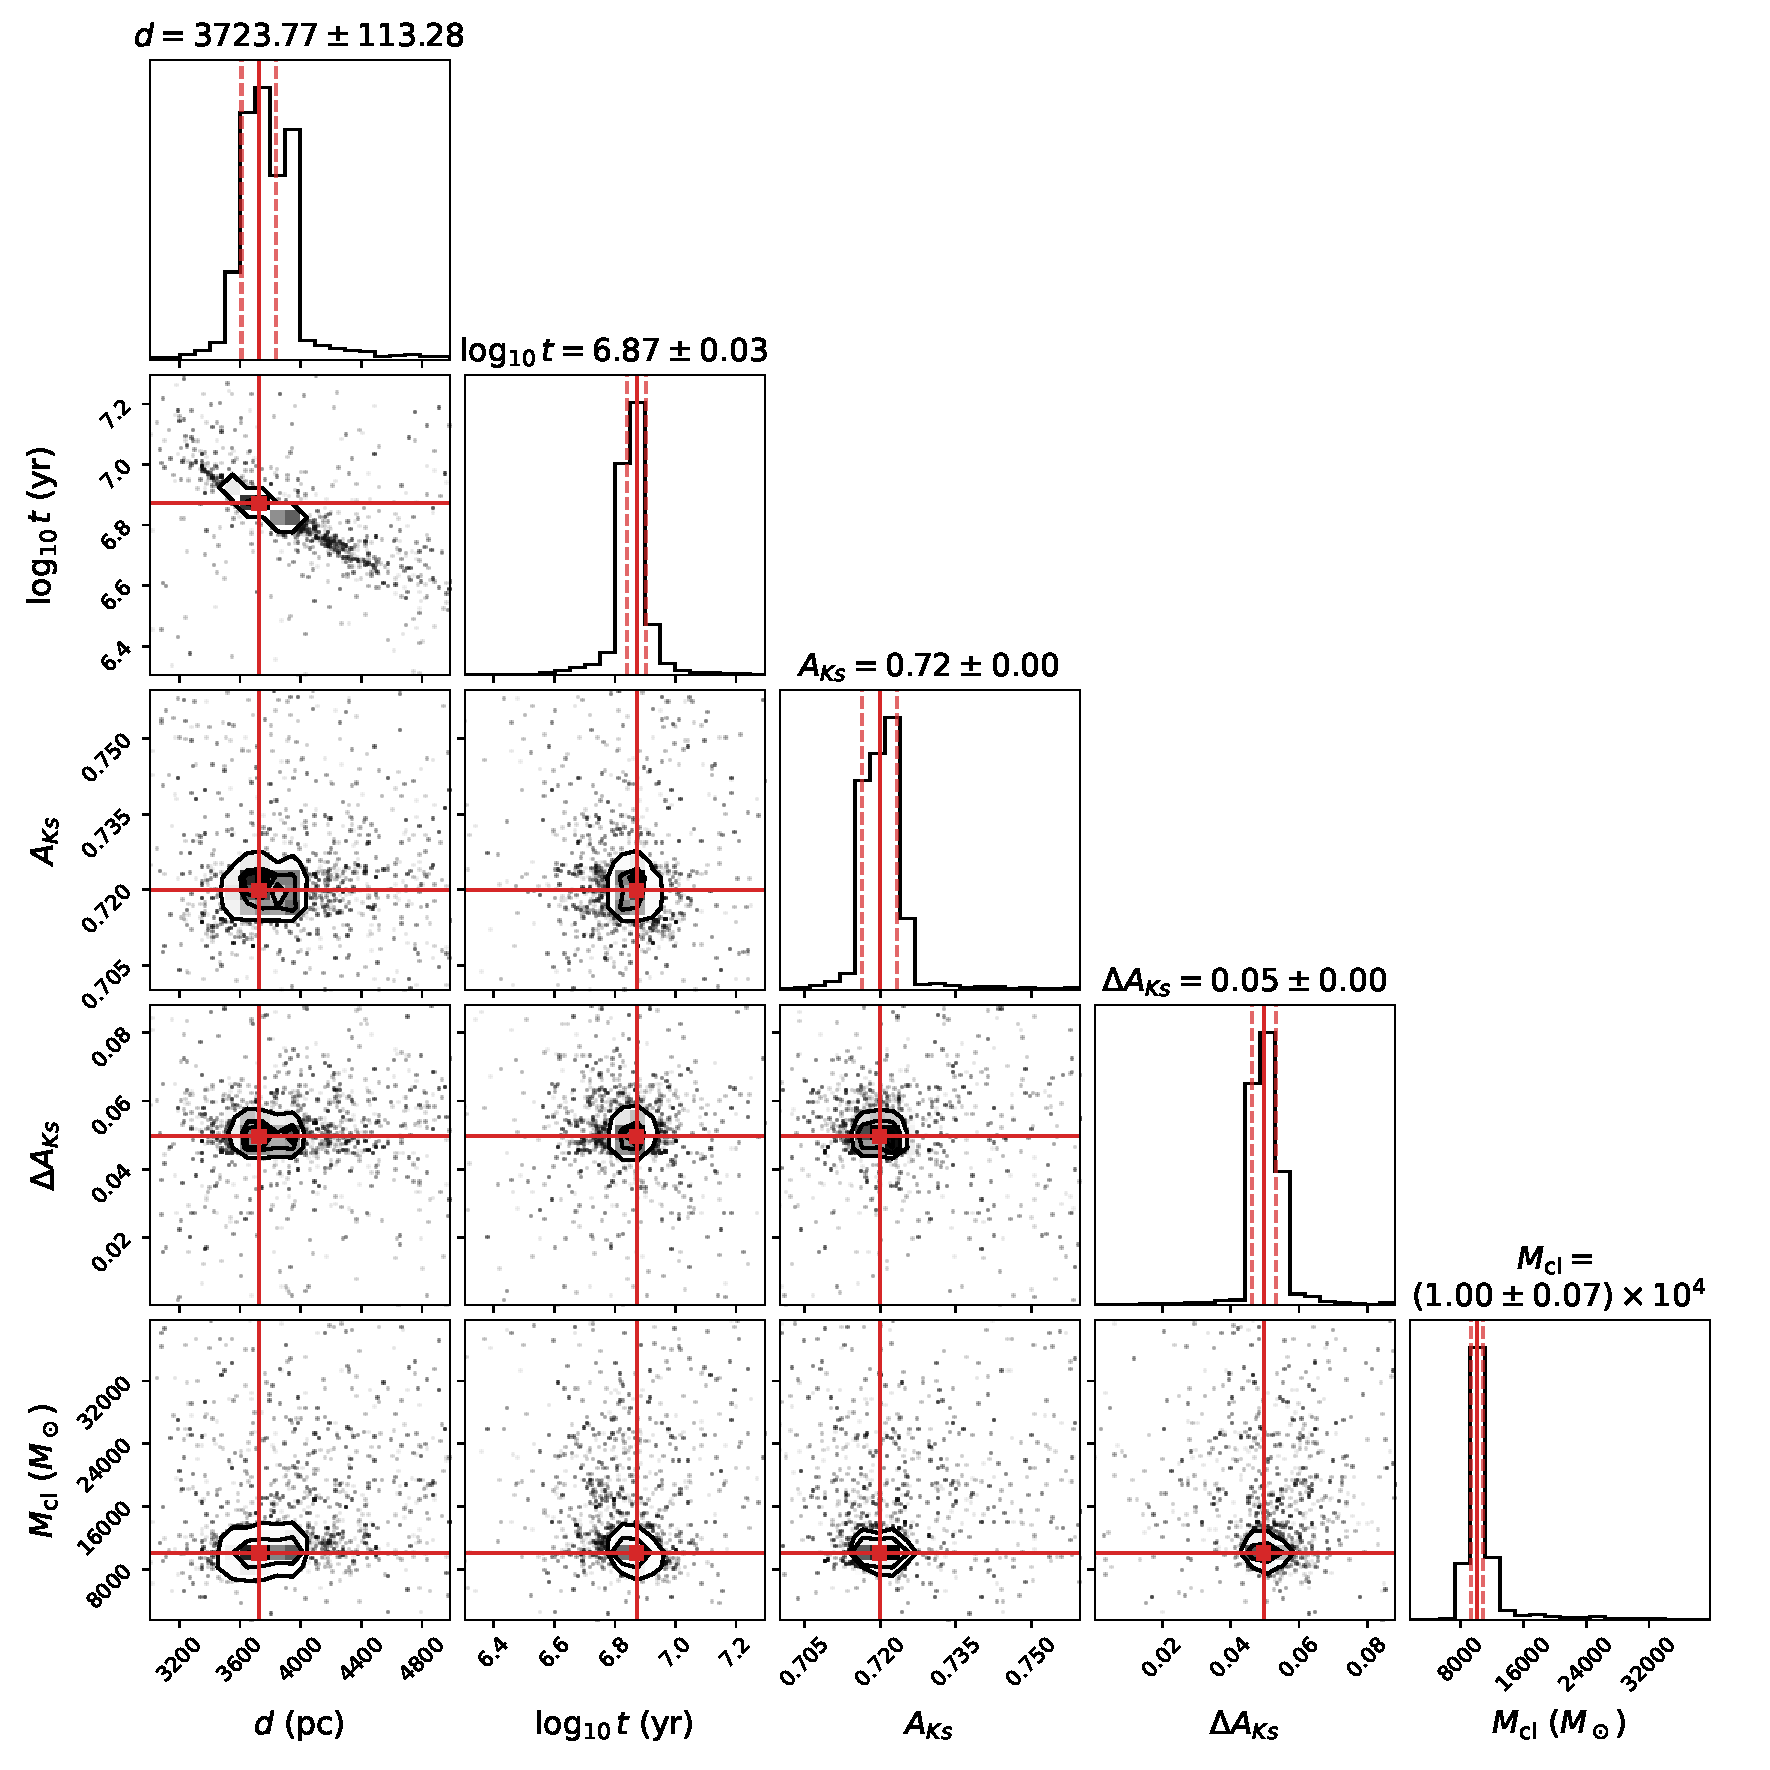
\includegraphics[width=0.7\linewidth]{figures/chapter2/imf_corner_marginalized.pdf}
    \caption[Posterior of the CMD fit]{Posterior of the CMD fit. The {\em red solid} lines mark the median of the burnt-in samplers, and the {\em red dashed} lines represent the $16$-th and $84$-th percentiles, or $1$-$\sigma$ uncertainties.}
    \label{fig:imf_corner_marginalized}
\end{figure}

With the posterior probability function described in Section~\ref{wd1-subsec:age_distance}, the best-fit cluster properties are determined utilizing the Markov chain Monte Carlo (MCMC) Ensemble sampler \texttt{emcee} \citep[][]{emcee} with uniform prior functions and distributions, $100$ samplers, $300$ steps, and the \texttt{KDEMove} proposal. The final $100$ converged steps are considered as the burnt-in steps and are used to determine the value and uncertainties of the parameters. We binned the CMD of the observed and best-fit simulated clusters and their difference for visualization comparisons in Figure~\ref{fig:cmd}. In this work, we focus on the constraints from the cluster age and distance, which are relevant for later discussions on velocity dispersion (Section~\ref{wd1-subsec:vdisp_result}) and mass segregation (Section~\ref{wd1-subsec:mass_segregation}). The marginalized posteriors of distance $d$, age $t$, extinction $AK_S$, and differential extinction $dAK_S$ are shown in Figure~\ref{fig:imf_corner_marginalized}. Additional free parameters in CMD modeling, such as the IMF slopes and break mass,  will be constrained more robustly with new observational data in an upcoming paper (L. Wei et al., in prep). The resulting best-fit cluster distance is $3723.77\pm113.28$~pc, and the age is $\log_{10}t = 6.87 \pm 0.03$, corresponding to $7.45 \pm 0.53$~Myr. The best-fit cluster age and distance were used to generate the isochrone shown in Figure~\ref{fig:3_panel_population} and interpolate the stellar masses.



\subsection{Velocity Dispersion}
\label{wd1-subsec:vdisp_result}

\begin{figure*}[htb!]
    \centering
    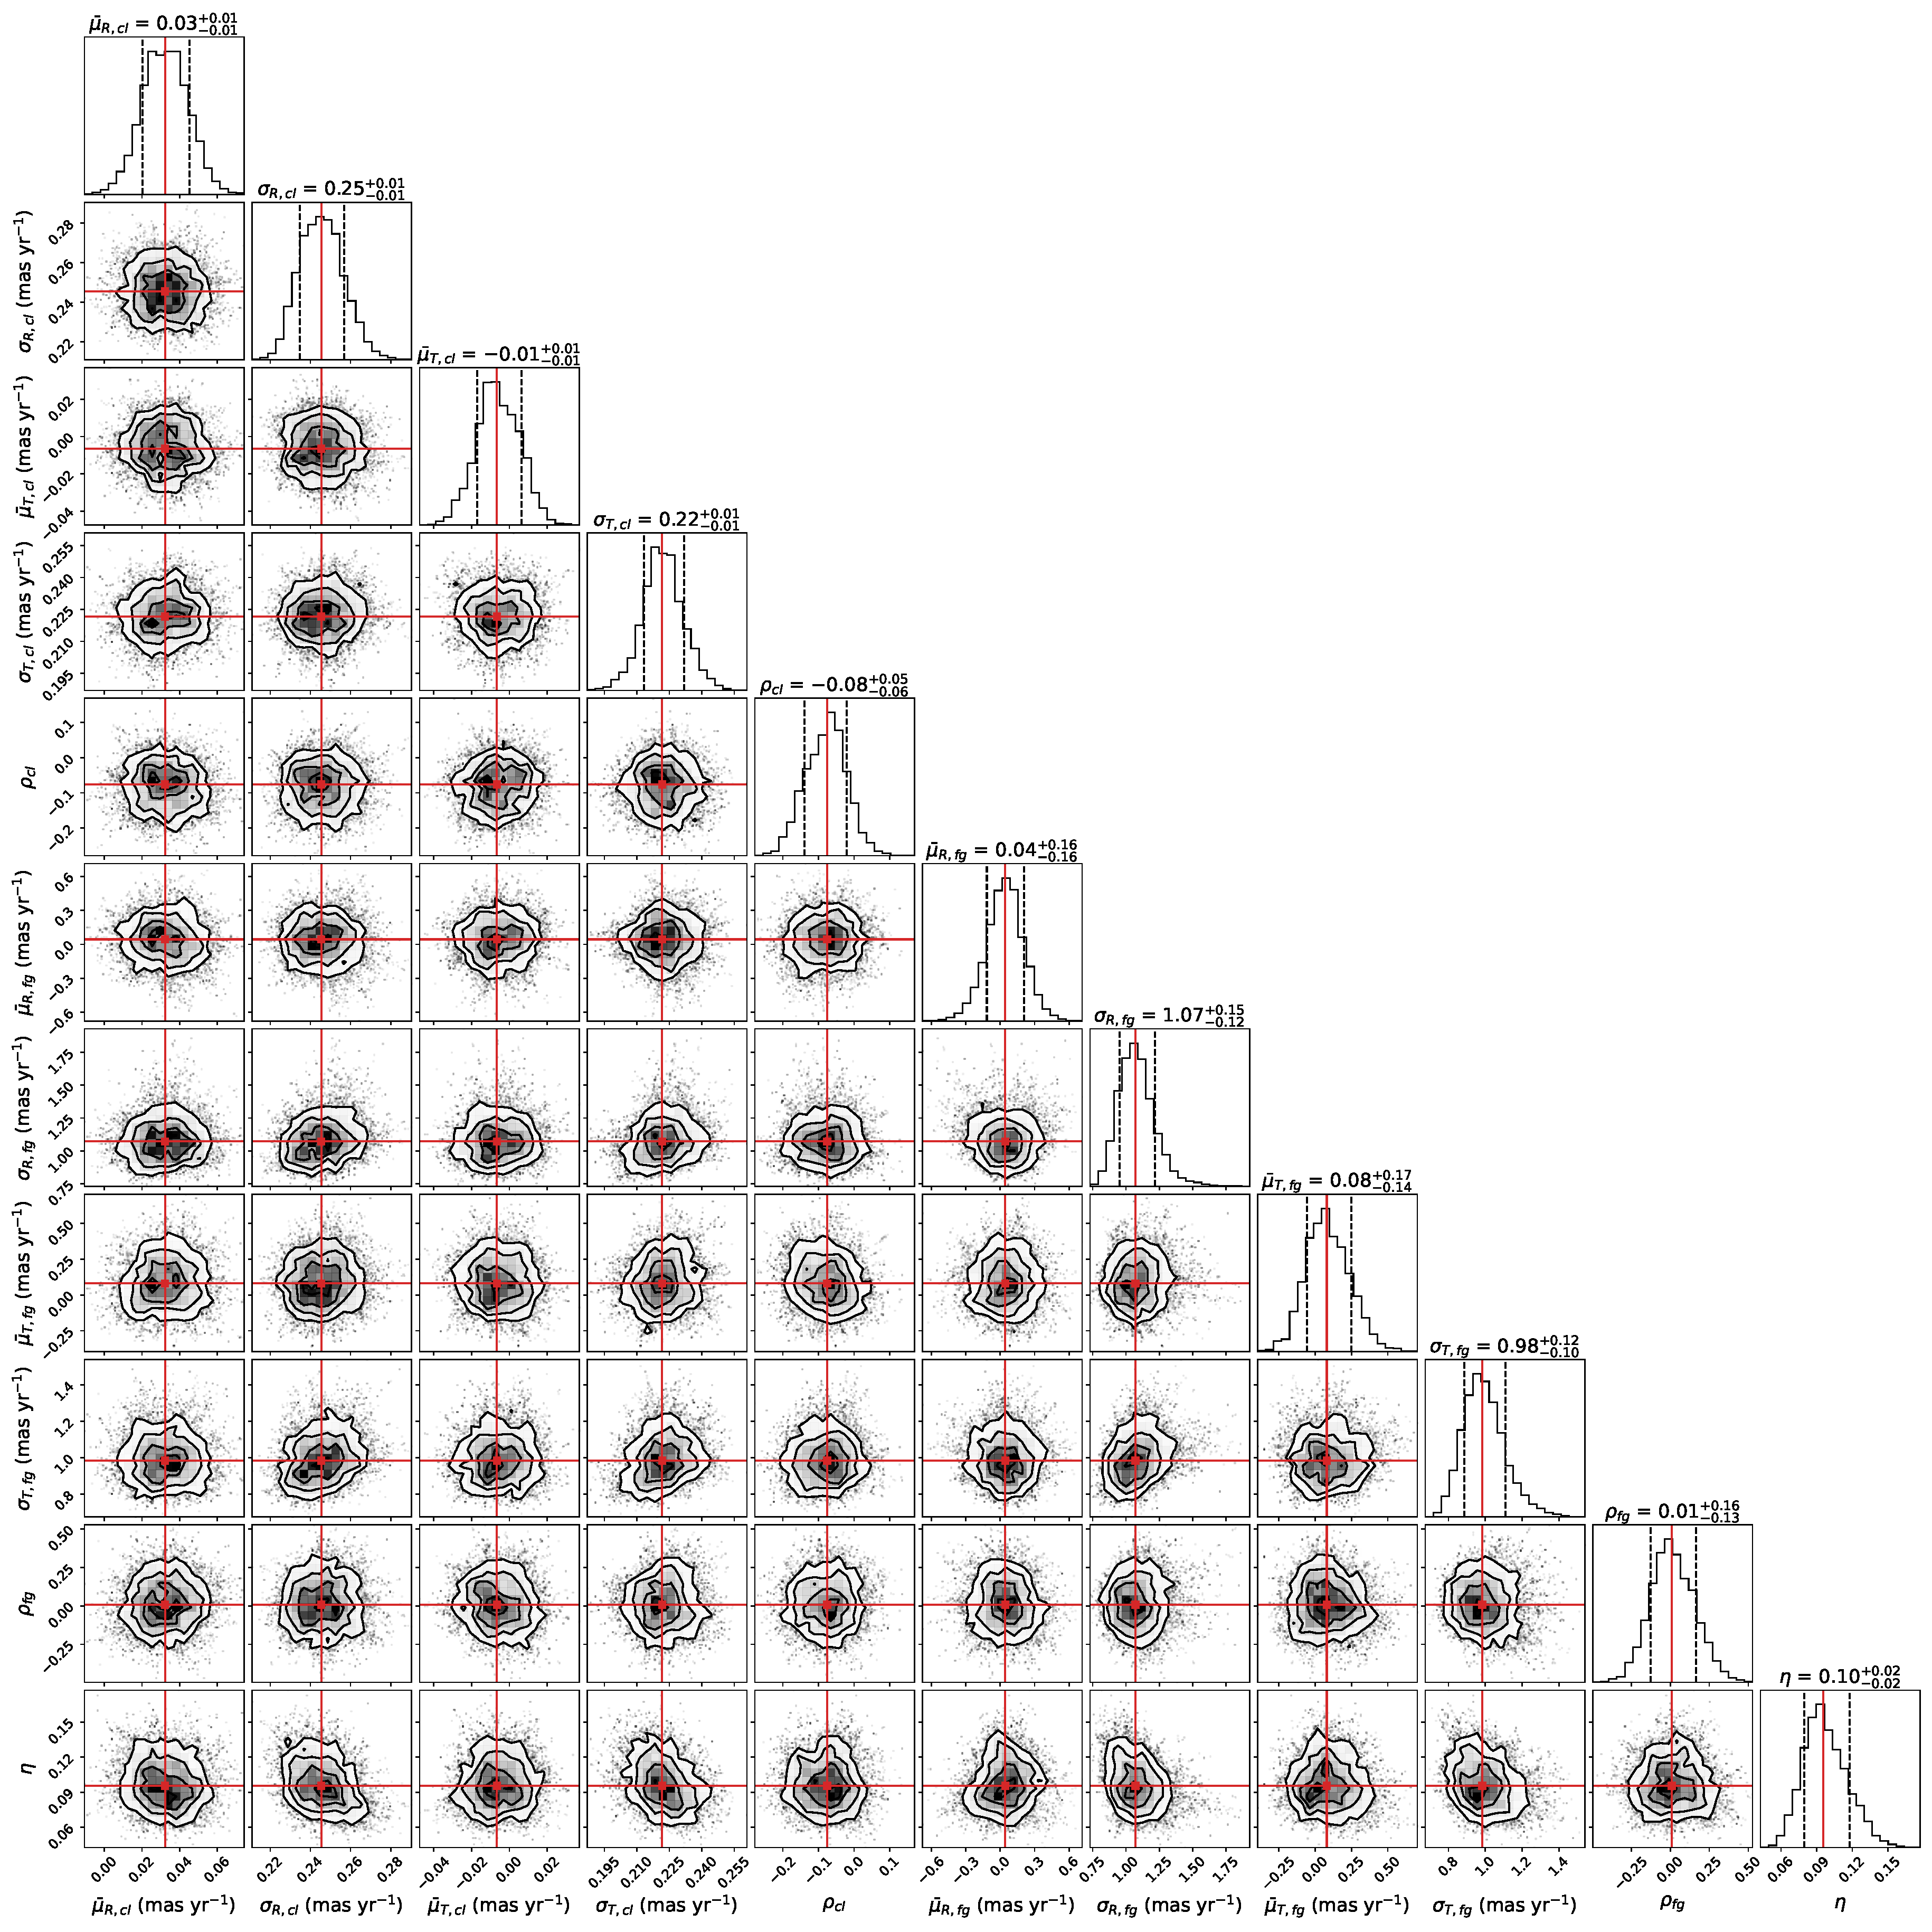
\includegraphics[width = \linewidth]{figures/chapter2/vdisp_corner.pdf}
    \caption[Posterior distributions of kinematics modeling]{Marginalized posterior distributions for the parameters of kinematic modeling. The red line marks the median, and the dashed vertical lines mark the $16$-th and $84$-th percentiles.}
    \label{fig:vdisp_corner}
\end{figure*}

We model the intrinsic PM velocity dispersion for the subsample by a mixture of two bivariate Gaussians, one for the cluster members (subscripted by $\mathrm{cl}$) and the other for the residual foreground stars (subscripted by $\mathrm
{fg}$). Each Gaussian is characterized by the mean PM values $\boldsymbol{\bar{\mu}} \equiv \left(\bar{\mu}_{R}, \bar{\mu}_{T}\right)$, the PM dispersions $\boldsymbol{\sigma} \equiv \left(\sigma_{R}, \sigma_{T}\right)$, and the correlation coefficient $\rho$. Given a set of PM measurements $D \equiv \lbrace \boldsymbol{\mu}_i, \boldsymbol{\epsilon}_i \rbrace_{i=1}^N$, where $\boldsymbol{\mu}_i \equiv \left(\mu_{R, i}, \mu_{T, i}\right)$ is the PMs of the $i$-th star, and $\boldsymbol{\epsilon}_i \equiv \left(\epsilon_{R, i}, \epsilon_{T, i}\right)$ is the associated uncertainties, the posterior for the Gaussian parameters $\boldsymbol{p_\mathrm{cl}} \equiv (\boldsymbol{\bar{\mu}}_\mathrm{cl}, \boldsymbol{\sigma_\mathrm{cl}}, \rho_\mathrm{cl})$ and $\boldsymbol{p_\mathrm{fg}} \equiv (\boldsymbol{\bar{\mu}}_\mathrm{fg}, \boldsymbol{\sigma_\mathrm{fg}}, \rho_\mathrm{fg})$ is:
\begin{equation}
P\left(\boldsymbol{p_\mathrm{cl}, \boldsymbol{p_\mathrm{fg}}} | D\right) \propto P\left(D | \boldsymbol{p_\mathrm{cl}, \boldsymbol{p_\mathrm{fg}}}\right) P\left(\boldsymbol{p_\mathrm{cl}}, \boldsymbol{p_\mathrm{fg}}\right)\,,
\end{equation}
according to the Bayes' theorem, where $P\left(D | \boldsymbol{p_\mathrm{cl}, \boldsymbol{p_\mathrm{fg}}}\right)$ is the likelihood and $P\left(\boldsymbol{p_\mathrm{cl}}, \boldsymbol{p_\mathrm{fg}}\right)$ is the prior. The likelihood $P(D|\boldsymbol{p_\mathrm{cl}, \boldsymbol{p_\mathrm{fg}}})$ is a product of the two Gaussian mixtures for each data point:
\begin{equation}
P(D|\boldsymbol{p_\mathrm{cl}, \boldsymbol{p_\mathrm{fg}}})  \propto \prod_{i}
\Bigl[(1-\eta)\,\mathcal{N}\left(\boldsymbol{\mu_i}; \boldsymbol{\bar{\mu}_\mathrm{cl}}, \Sigma_{cl, i}\right) + \eta~\mathcal{N}\left(\boldsymbol{\mu_i}; \boldsymbol{\bar{\mu}_\mathrm{fg}}, \Sigma_{fg, i}\right)\Bigr],
\end{equation}
where $\eta$ is the fraction of the foreground contaminants, $\mathcal{N}\left(\boldsymbol{\mu_i}; \boldsymbol{\bar{\mu}}, \Sigma_i\right)$ denotes the probability density function of a bivariate normal distribution characterized by a mean of $\boldsymbol{\bar{\mu}}$ and covariance of $\Sigma_i$ evaluated for the $i$-th star with measured PMs $\boldsymbol{\mu_i}$. The covariance matrices of the $i$-th star $\Sigma_{cl, i}$ and $\Sigma_{fg, i}$ are associated with the measurement errors and intrinsic kinematics of the cluster and the foreground population, respectively:
\begin{equation}
\Sigma_{cl, i} = \begin{bmatrix} \sigma_{R, \mathrm{cl}}^2 + \epsilon_{R, i}^2 & \rho_\mathrm{cl}\,\sigma_{R, \mathrm{cl}}\,\sigma_{T, cl}\\ \rho_\mathrm{cl}\,\sigma_{R, \mathrm{cl}}\,\sigma_{T, cl} & \sigma_{T, cl}^2 + \epsilon_{T, i}^2 \end{bmatrix},
\end{equation}
\begin{equation}
\Sigma_{\mathrm{fg}, i} = \begin{bmatrix} \sigma_{R, \mathrm{fg}}^2 + \epsilon_{R, i}^2 & \rho_\mathrm{fg}\,\sigma_{R, \mathrm{fg}}\,\sigma_{T, \mathrm{fg}}\\ \rho_\mathrm{fg}\,\sigma_{R, \mathrm{fg}}\,\sigma_{T, \mathrm{fg}} & \sigma_{T, \mathrm{fg}}^2 + \epsilon_{T, i}^2 \end{bmatrix}.
\end{equation}
In the case of the prior $P(\boldsymbol{p_\mathrm{cl}}, \boldsymbol{p_\mathrm{fg}})$, we adopt the non-informative Jeffreys priors for each bivariate Gaussian as follows \citep{Berger-2008, Bernardo-1988}:

\begin{equation}
P(\boldsymbol{p_\mathrm{cl}}, \boldsymbol{p_\mathrm{fg}}) \propto \frac{1}{\sqrt{(1-\eta)\,\eta}} \prod_{k=\mathrm{cl}, \mathrm{fg}}\left[\sigma_{R, k}\,\sigma_{T, k}\left(1-\rho_{k}^2\right)\right]^{-2}
\end{equation}

We restrict the velocity dispersion modeling to a subsample of member candidates with high-quality PM measurements. The selection criteria are listed as follows:
\begin{enumerate}[leftmargin=*, label=\roman*., align=left, labelsep=0em, itemsep=0em]
    \item Synthetic PM measurement errors smaller than $0.2~\rm mas\,yr^{-1}$;
    \item Color membership cuts illustrated Figure~\ref{fig:color_membership};
    \item Dereddened $\mathrm{F160W_D}$ brighter than  $16$~mag.
\end{enumerate}
The kinematic membership probabilities are not involved in the subsampling process, which would otherwise bias the velocity dispersions in favor of smaller values. Instead, criteria ii and iii are adopted to minimize the fraction of foreground stars while ensuring completeness across the FOV. By these criteria, \num{1204} stars are selected, whose PMs are then transformed from $x$--$y$ coordinates to radial ($R$) and tangential ($T$) components.

We sample the posterior $P(\boldsymbol{p_\mathrm{cl}, \boldsymbol{p_\mathrm{fg}}}|D)$ with \texttt{emcee} \citep[][]{emcee} and present the marginalized distributions of each parameter in 
Figure~\ref{fig:vdisp_corner}. Note that using uniform priors instead of the Jeffreys priors does not significantly impact our result. The fraction of foreground contaminants is estimated as low as $\sim10 \pm 2\%$. 

The mean PM in the radial and tangential component are $\left(\mu_{R, \mathrm{cl}}, \mu_{T, cl}\right) =\linebreak[4] (0.03 \pm 0.01, -0.01 \pm 0.01)~\mathrm{mas}\,\mathrm{yr}^{-1}$, translating into $\left(0.57 \pm 0.22, -0.12 \pm 0.21\right)~\mathrm{km}\,\mathrm{s}^{-1}$ at a distance of $3723.77$~pc, with positive tangential component corresponding to the counter-clockwise direction. The radial component is consistent with zero within $3$-$\sigma$, indicating the positive value is statistically insignificant. The radial PM is not found to increase with the radius from the cluster center either. Therefore, we find no evidence of expansion or contraction in the cluster, favoring the static scenario proposed by \citet{Gennaro-2017}. 

The velocity dispersion measures to be $(\sigma_{R, \mathrm{cl}},\sigma_{T, cl}) = (0.25 \pm 0.01,\linebreak[4] 0.22 \pm 0.01)~\rm mas\,yr^{-1}$, equivalent to $(4.33 \pm 0.19, 3.91 \pm 0.16)~\mathrm{km}\,\mathrm{s}^{-1}$ at the best-fit heliocentric distance $3723.77$~pc. The 1D velocity dispersion is 
\begin{equation}
    \sigma_\mathrm{1D} = \sqrt{\frac{\sigma_{R, cl}^2 + \sigma_{T, cl}^2}{2}} = 4.13 \pm 0.13~\mathrm{km}\,\mathrm{s}^{-1}\,,
    \label{eq:vdisp_1d}
\end{equation}
or equivalently $0.23 \pm 0.01~\mathrm{mas}\,\mathrm{yr}^{-1}$. We compare the velocity dispersion with the virial equilibrium model in Section~\ref{wd1-subsec:virial state}.



\subsection{Mass Segregation}
\label{wd1-subsec:mass_segregation}

\begin{figure*}[htb!]
\centering
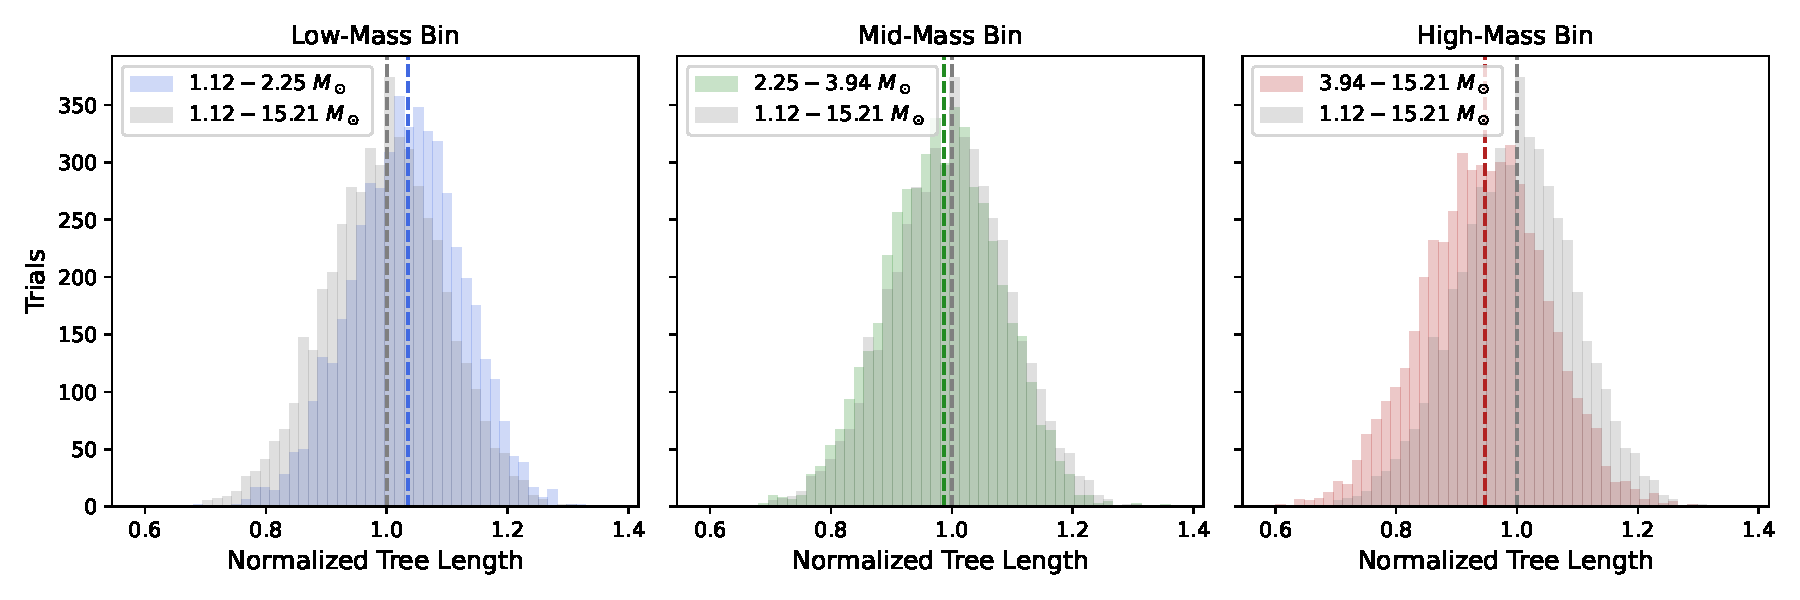
\includegraphics[width=\linewidth]{figures/chapter2/mst_trails_3_panel_5000_25.pdf}
\caption[Distribution of minimum spanning tree lengths]{Distribution of MST lengths for our low-, mid-, and high-mass bins normalized by the mean MST length of the full catalog. \textit{Left}: Low-mass bin. \textit{Middle}: Mid-mass bin. \textit{Right}: High-mass bin.}
\label{fig:mst_length}
\end{figure*}

\begin{figure}[htb!]
    \centering
    \includegraphics[width=0.7\linewidth]{figures/chapter2/minimum_spanning_tree.pdf}
    \caption[Minimum spanning tree in each mass bin]{Minimum spanning tree in each mass bin with a tree length closest to the median normalized tree length in Figure~\ref{fig:mst_length}. The high-mass stars are marked with {\em red x's}, the mid-mass stars are marked by {\em green triangles} and connected by {\em green dashed lines}, and the low-mass objects are marked with {\em blue circles} connected by {\em blue dotted lines}.}
    \label{fig:mst}
\end{figure}

We investigate mass segregation in the cluster with two metrics: the mass segregation ratio and the core radii of the radial profiles from Section~\ref{wd1-subsec:radial_profile}.

We model mass segregation in the cluster using the
mass segregation ratio, $\Lambda_{\rm MSR}$, developed by \citet{Allison-2009}, which is recognized as a reliable approach with the advantage of not requiring a center or overall stellar distribution \citep[see][for further discussions]{Parker-2015}. This method examines the degree of mass segregation by a ratio of the Minimum Spanning Tree (MST) length connecting the $N_\mathrm{MST}$ most massive stars, $l_{Massive}$, to the mean MST length of $N_\mathrm{MST}$ random stars, $\langle l_{norm} \rangle$. The distribution of $\langle l_\mathrm{norm} \rangle$ is roughly Gaussian, and the error $\sigma_\mathrm{norm}$ is then taken to be the standard deviation of the distribution. 
The mass segregation ratio $\Lambda_\mathrm{\rm MSR}$ is defined as:
\begin{equation}
     \Lambda_\mathrm{\rm MSR} = \frac{\langle l_\mathrm{norm} \rangle}{l_\mathrm{Massive}} \pm \frac{\sigma_\mathrm{norm}}{l_\mathrm{Massive}}~.
\end{equation}
When $\rm \Lambda_{\rm MSR}$ significantly differs significantly from $1$, there is either mass segregation or inverse mass segregation for values $> 1$ or $< 1$, respectively. A value of $1$ indicates no mass segregation in the cluster.  

We modify this method by finding the distribution of $l_{Massive}$ in a set of massive stars, rather than setting a fixed value of $N_\mathrm{MST}$ massive stars. We randomly sample this set of massive stars in the same way we sample the random set of stars, and then compare the distributions of the MST length. In this way, we can characterize the distribution of minimum separations of the massive stars more comprehensively.  Our updated mass segregation ratio is defined as:
\begin{equation}
        \rm \Lambda_\mathrm{\rm MSR} = \frac{\langle l_\mathrm{norm} \rangle}{\langle l_\mathrm{Massive} \rangle} \pm \sigma_\mathrm{\rm MSR}\,,
\end{equation}
where
\begin{equation}
        \rm \sigma_{\rm MSR} = \frac{\langle l_{norm} \rangle}{\langle l_{Massive} \rangle}     \sqrt{\bigg(\frac{\sigma_{norm}}{\langle l_{norm} \rangle}\bigg)^2 + \bigg(\frac{\sigma_{Massive}}{\langle l_{Massive} \rangle}\bigg)^2}~.
\end{equation}
We utilize \texttt{scipy} to construct the MST. To ensure a smooth distribution of MST lengths, we perform $5000$ trials of $25$ randomly chosen stars for both sets of stars. All populations are comprised of cluster members with $\pclust \geq 0.3$. We account for the weight of each star by assigning the likelihood of selecting a given star proportional to its weight, as defined in Equation~\eqref{eq:weight}. 

Using the $200$ brightest stars with $\mathrm{F160W}_\mathrm{D} \leq 13.6$ ($\gtrapprox5.4~M_\odot$) in our sample as the set of massive stars, we find $\rm \Lambda_{\rm MSR} = 1.11\pm0.11$, slightly greater than $1$ by only $1\sigma$. We also notice that the mean MST lengths tend to decrease as the mean stellar mass increases, as shown in Figure~\ref{fig:mst_length}, where we show the distributions of the MST length normalized by the mean of the full catalog for three mass bins. Figure~\ref{fig:mst} illustrates the MST of each mass bin closest to the median of their corresponding tree lengths.

A similar trend is found in the posterior distributions of $r_c$ in the EFF radial profile modeling, as shown in Figure~\ref{fig:mass_binned_radial_profile} Two-sided Kolmogorov--Smirnov (KS) tests comparing the radii of the stars in each mass bin also indicate that they are drawn from different parent distributions. The $p$-values corresponding to the low-intermediate, low-high, and intermediate-high mass bin comparisons are \num{1.81e-2}, \num{3.14e-3}, and \num{3.08e-9}, respectively, all of which are smaller than \num[]{5e-2}. We therefore reject the null hypothesis that the radii are drawn from the same distribution and conclude that there is a low level of mass segregation present in the cluster within our mass range.


\section{Discussion}
\label{wd1-sec:discussion}
With the structural and kinematic information derived in this work, we discuss the virial state, the relevant timescales of the cluster, and their implications.

\subsection{Elongation}
\label{wd1-subsec:elongation}

\begin{figure}[htb!]
    \centering
    \includegraphics[width=0.7\linewidth]{figures/chapter2/eccentricity.pdf}
    \caption[Eccentricity of the stellar density Gaussian profile]{Eccentricity of the stellar density Gaussian profile as a function of stellar mass. 
    The blue line shows the results of this study. The green dashed line and the shaded region mark the value and uncertainty derived in \citet{Muno-2006}. The amber line shows the measurements in \citet{Brandner-2008}. The overall eccentricity claimed by \citet{Gennaro-2011} is marked as the red dotted line.}
    \label{fig:eccentricity}
\end{figure}

Our measured eccentricity of $0.71$ is in good agreement with the value of $0.75$ reported by \citet{Gennaro-2011} and falls within the range of $0.68$––$0.72$ identified by \citet{Andersen-2017}. \citet{Muno-2006} reported a similar value of $e=0.66 \pm 0.02$ by measuring the diffuse X-ray emissions of the cluster. In addition, we find the eccentricity decreases slightly with increasing mass, with $e=0.75$, $0.67$, and $0.65$ for the low-, mid-, and high-mass bins, respectively, a trend that aligns with the findings of \citet{Gennaro-2011}. \citet{Brandner-2008} measured a moderately smaller $e$ of $0.53$ and $0.59$ for the mass ranges of $3.5$--$10~M_\odot$ and $10$--$32~M_\odot$, respectively. The smaller eccentricity may stem from the bias introduced by the authors' assumption about a point-symmetric half-mass radius. Instead, our measurement did not impose any assumption on the mass distribution. Different definitions of eccentricity and ellipticity are employed in the literature. In this work, we adopted the definition of ellipticity and eccentricity as described in Section~\ref{wd1-subsec:density_modeling}. For consistency, we transformed the literature values to align with this definition for comparison. Figure~\ref{fig:eccentricity} shows the comparison of values measured in this study and the literature. 

The observed high eccentricity may result from the morphology of the molecular cloud within which Wd1 forms, or imply a hierarchical formation pathway involving the merger of multiple substructures. The decreasing trend of eccentricity with increasing mass can be attributed to the shorter dynamical timescale of more massive stars as they are more concentrated in the center, which can be clearly observed in Figure~\ref{fig:2D_density_map}. Therefore, more frequent interactions result in a more isotropic profile. Furthermore, as the elongation aligns with the galactic plane, this could also arise from the tidal stripping along the plane of less massive stars on the periphery of the cluster.



\subsection{Virial State}
\label{wd1-subsec:virial state}
Our measured velocity dispersion of $4.13\pm0.13~\mathrm{km}\,\mathrm{s}^{-1}$ is slightly smaller than the values expected for the cluster if it were in virial equilibrium $\sigma_\mathrm{vir}=4.5$--$6.5~\mathrm{km}\,\mathrm{s}^{-1}$, suggesting that the cluster is close to subvirial. \citet{Brandner-2008} estimated the virial equilibrium velocity dispersion to be $\sigma_\mathrm{vir} \geq 4.5~\mathrm{km}\,\mathrm{s}^{-1}$, or $0.25~\mathrm{mas}\,\mathrm{yr}^{-1}$ at their distance estimate of $3.55$~kpc.  \citet{Gennaro-2011} and \citet{Gennaro-2017} estimates $\sigma_\mathrm{vir}=4.5^{+0.8}_{-0.2}~\mathrm{km}\,\mathrm{s}^{-1}$, and \citet{Negueruela-2010} reported $6.5~\mathrm{km}\,\mathrm{s}^{-1}$ (see \citealp{Cottaar-2012} for details). Note that the equilibrium velocity dispersion estimates depend on IMF extrapolations, which need further confirmation. The viral velocity estimate would benefit from a more complete sample of low-mass objects in Wd1. Distance is another factor affecting the virial state. Wd1 would be in

Assuming the current estimate of virial equilibrium velocity dispersion, Wd1 would need to be at a distance of $4.0$--$5.8$~kpc instead of $3077$~pc for the observed velocity dispersion to match the virial equilibrium model. 

The subvirial state of the Wd1 cannot be definitively confirmed with the uncertainties in the IMF extrapolation and distance estimates.


In comparison, \citet{Mengel-2007} measured $\sigma_\mathrm{1D}=9.2\pm2.5~\mathrm{km}\,\mathrm{s}^{-1}$ from $4$ red supergiants, $5$ yellow hypergiants, and a B-type
emission line star. However, this result may be highly overestimated due to the presence of binaries \citep[e.g.,][]{Kouwenhoven-2008, Gieles-2010}. \citet{Cottaar-2012} reported $2.1^{+3.3}_{-2.1}~\mathrm{km}\,\mathrm{s}^{-1}$, which is derived from the spectroscopic measurements of several PMS stars. Our velocity dispersion measurement is derived from a significantly larger sample with membership and completeness correction. These improvements help mitigate potential biases and enhance the reliability and robustness of our results.


At the age of Wd1, mass loss due to radiative feedback has already occurred, and the cluster should be dynamically responding. If present, the subvirial state of Wd1 with little gas remaining may imply that the star formation efficiency (SFE, the fraction of the initial gas mass that is turned into stars) is high enough at its formation for it to survive as a bound cluster. Previous studies find that eventually bound clusters are more likely to form in exceptionally high SFE environments, typically greater than $50\%$ \citep[][]{Geyer-2001, Li-2019}. However, there are arguments that up to half of the stars can remain bound with SFE smaller than $50\%$ \citep[][]{Boily-2003}.

Alternatively, cluster formation mechanisms can also explain the gravitationally bound state of Wd1. Instead of forming in a static molecular cloud, stars can form in local overdensities such as gas filaments before they reach the forming star cluster \citep[][]{Bonnell-2008, Longmore-2014, Wei-2024}. Gas expulsion that already happens locally reduces the negative influence of stellar feedback on new star formation, resulting in bound clusters free of gas \citep[][]{Kruijssen-2012, Krause-2020, Chevance-2023}. The high eccentricity of $e=0.71$ of Wd1 identified in this work may result from the merging of such local substructures during its formation.



\subsection{Radial Profile Comparisons}
\label{wd1-subsec:arches_quint}

\begin{figure*}[htb!]
\centering \includegraphics[width=\linewidth]{figures/chapter2/arches_quint_comparison_sub_b.pdf}
\caption[Comparison of the Westerlund 1 radial density profile to the Arches and Quintuplet]{Comparison of the radial profile of Wd1 to the Arches and Quintuplet clusters using the EFF fit parameters in \citet{Hosek-2015} and \citet{Rui-2019}. We restrict the profile fit to $M \geq 4.5~M_\odot$ and $M \geq 2.5~M_\odot$ for the Arches and Quintuplet comparison, respectively.}
% \textcolor{red}{Nicholas: Matt actually reran the Arches profile at the same mass limits as the Quintuplet analysis in my paper, so maybe you can use that and combine these two subplots together... would make a nice, succinct key plot showing all three clusters on top of each other}}
\label{fig:arches_quint_radial_profile_comparison}
\end{figure*}


\begin{figure*}
    \centering
    \gridline{
        \fig{figures/chapter2/EFF_posteriors_arches.pdf}{0.491\linewidth}{(a) Arches Comparison: Wd1 $M \geq 4.5~M_\odot$}
        \fig{figures/chapter2/EFF_posteriors_quint.pdf}{0.491\linewidth}{(a) Quintuplet Comparison: Wd1 $M \geq 2.5~M_\odot$}
    }
    \caption[Posteriors of radial profile comparisons]{Weighted posterior distributions of EFF radial profile parameters. (a): Sources with mass greater than $4.5~M_\odot$ for comparison with the Arches cluster. (b): Sources with mass greater than $2.5~M_\odot$ for comparison with the Quintuplet cluster. The red lines mark the weighted median, and the gray dashed line marks the weighted $16$- and $84$-th percentiles. Note that we only modeled $r_c$, and the posterior distribution of $a$ is purely converted from $r_c$.}
    \label{fig:radial_profile_posteriors_arches_quint}
\end{figure*}

We compare the radial density profile of Wd1 with those of the Arches and Quintuplet clusters, modeled using the same methodology. We set a minimum mass limit of $4.5~M_\odot$ and $2.5~M_\odot$ to keep consistent mass ranges with Arches and Quintuplet, respectively. Details regarding the numbers of unweighted and weighted stars per bin and bin edges in mass are provided in Table~\ref{wd1-tab:cluster_statistics}.

Figure~\ref{fig:arches_quint_radial_profile_comparison} shows the EFF radial profile comparisons with the Arches and Quintuplet, respectively. For consistency of comparisons, the masses are restricted to $\geq4.5~M_\odot$ and $\geq2.5~M_\odot$. The associated posteriors are illustrated in Figure~\ref{fig:radial_profile_posteriors_arches_quint}. The Arches cluster displays a stellar density more than $10$ times denser than the Wd1 in the core, while the Quintuplet cluster shares a similar density profile and core radius with Wd1.


\subsection{Dynamical Timescales}
\label{wd1-subsec:timescales}
In this section, we discuss the crossing time, relaxation time, the expected mass segregation timescales, and their implications on whether the mass segregation in Wd1 is dynamical or primordial. 

The crossing time of Wd1 is
\begin{equation}
    t_\mathrm{cross} = \frac{r_\mathrm{hm}}{\sigma_\mathrm{1D}} = 0.26~\mathrm{Myr}\,,
\end{equation}
where we adopted the half-mass radius of $r_\mathrm{hm}=1.17$~pc corrected by completeness and area fraction, after excluding stars with an area fraction $f<0.3$ used in modeling the velocity dispersion as in Section~\ref{wd1-subsec:vdisp_result}. This is consistent with the half-mass radius used in \citet{Brandner-2008}. In comparison, \citet{Gennaro-2017} estimated a crossing time of $0.2$~Myr assuming Wd1 is virialized with a full radius of $2$~pc. Our estimate results directly from the velocity dispersion measurements, without any assumption about the virial state. The age of Wd1 is therefore about $36$ times its crossing time.

The relaxation time can be calculated from the number of stars $N$ and the crossing time $t_\mathrm{cross}$ \citep[][]{Binney-2008},
\begin{equation}
    t_\mathrm{relax} = \frac{N}{10\ln N} t_\mathrm{cross} = 0.22~\mathrm{Gyr}\,,
\end{equation}
where we assume the total number of stars is $N\sim10^5$ \citep[][]{Brandner-2008, Gennaro-2017}. This is about $30$ times the age of Wd1.

The timescale for a star of mass $M$ to reach energy equipartition and therefore dynamical mass segregation is
\begin{equation}
    t(M)\sim\frac{\overline{m}}{M}t_\mathrm{relax}\,,
\end{equation}
where $\overline{m}$ is the average mass of the cluster. Considering the cluster age of $7.45~\mathrm{Myr}$ and an average mass of $\sim0.4~M_\odot$ \citep[][]{Gennaro-2017}, we would expect mass segregation for stars more massive than $\sim12~M_\odot$. In comparison, \citet{Cottaar-2012} estimated a segregation mass of $20~M_\odot$, and \citet{Gennaro-2017} reported little or no mass segregation except for the $>40M_\odot$ stars in Wd1 based on observation. Recall that our analysis is restricted to stars in the mass range of $1.12$--$15.21~M_\odot$, which accounts for the low-level segregation observed in this study. With a mass segregation ratio of $\Lambda_\mathrm{MSR}=1.11 \pm 0.11$, only marginally greater than $1$ by $1$--$\sigma$. This is consistent with the expectation from the timescale analysis that the stellar population in this mass range does not exhibit strong segregation.

The consistency between the observed minor mass segregation in the lower mass range, combined with the segregation mass estimates based on dynamical timescales, implies that the segregation in Wd1 is likely dynamical rather than primordial, in agreement with previous studies \citep[][]{Gennaro-2017}. Considering its age and relaxation timescale, the dynamical process in this mass range is possibly still ongoing. The highest-mass stars are already segregated, and lower-mass stars are beginning to experience the effects of dynamical processes, therefore displaying a weak sign of mass segregation.


\section{Conclusion}
\label{wd1-sec:conclusion}
We analyze the kinematics and structure of Wd1 using the multi-epoch astrometric and photometric data from HST WFC3-IR filters. We model the kinematic and color membership of the stars. The structure of Wd1 is thoroughly analyzed after correcting for membership, extinction, and completeness. Specifically, we report the following conclusions.
\begin{enumerate}[label=\roman*.]
    \item We obtained the cluster membership of \num{10346} observed stars, consisting of PM kinematic membership characterized by a 3-component GMM model, a boolean photometric membership, and completeness correction.
    \item We construct the stellar density map of Wd1 corrected by a spatial reddening map and cluster membership of each star.
    \item With the stellar density map, we find that the cluster is elongated in a northeast-southwest direction, with an eccentricity of $0.71$ and the semi-major axis at a position angle of $\sim$\ang{56} east of north. The elongation aligns with the galactic plane. Furthermore, eccentricity decreases with increasing mass.
    \item The high eccentricity may be inherited from the molecular cloud from which Wd1 formed, or imply a formation process during which multiple substructures merged. The alignment of the elongation with the galactic plane, coupled with the higher eccentricity and more spatially diffuse distribution of low-mass stars, may also indicate tidal disruption within the galactic plane.
    \item We fit an EFF radial profile model to the stellar density and observed a slight decrease in the core radius with increasing stellar mass, indicative of a minor mass segregation.
    \item Another weak sign of mass segregation is identified by comparing the MST length for different mass ranges, with a relatively small mass segregation ratio of $\rm \Lambda_{\rm MSR} = 1.11\pm0.11$.
    \item We present the velocity dispersion measurements for \num{1211} stars. The velocity dispersion is $(\sigma_{R, \mathrm{cl}},\sigma_{T, cl})=\left(0.25 \pm 0.01, 0.22 \pm 0.01\right)~\rm mas\,yr^{-1}$, translating into $(4.33 \pm 0.19, 3.91 \pm 0.16)~\mathrm{km}\,\mathrm{s}^{-1}$. The 1D velocity dispersion of $\sigma_\mathrm{1D} = 4.13 \pm 0.13~\mathrm{km}\,\mathrm{s}^{-1}$ is slightly below the virial equilibrium estimate of $\sigma_\mathrm{vir}=4.5$--$6.5~\mathrm{km}\,\mathrm{s}^{-1}$ reported in the literature, suggesting the cluster is on the verge of subvirial. This conclusion is subject to uncertainties in the distance and IMF extrapolations.
    \item The subvirial, gravitationally bound state of Wd1 with little gas remaining implies either an exceptionally high SFE likely $>50\%$ at its formation, or it forms from the merging of substructures like gas filaments that already started local gas expulsion driven by stellar feedback before they reach the cluster.
    \item The crossing time is $0.26$~Myr with a mean projected cluster radius of $R=1.0$~pc weighted by membership, completeness, and area fraction. The age of Wd1 at $7.45$~Myr is about $29$ times its crossing time. The relaxation time is $0.22$~Gyr, about $30$ times its age.
    \item Given the age and relaxation time, we expect mass segregation for stars down to $12~M_\odot$, which accounts for the weak sign of segregation in our analysis with $\Lambda_\mathrm{MSR}=1.11\pm0.11$, as this work is restricted to sources between the mass range of $1.12$--$15.21~M_\odot$. This implies that mass segregation is more likely dynamical rather than primordial in Wd1.
\end{enumerate}

\facility{HST WFC3}
\software{
    \texttt{astropy} \citep[][]{Astropy-2018, Astropy-2022},
    \texttt{emcee} \citep[][]{emcee},
    \texttt{Matplotlib} \citep[][]{Matplotlib}
}

\section*{Acknowledgement}
Chapter~\ref{chapter:onc}, in full, is a reprint of the material as it appears in the Astrophysical Journal, \citealt{Wei-2024}.


\chapter{The Unusual Initial Mass Function of Westerlund 1}
\label{chapter:imf}
The initial mass function (IMF) is an empirical function that describes the distribution of stellar birth masses in a star-forming region and is critical to understanding processes ranging from star formation to galaxy evolution. Previous observations have found the shape of the IMF surprisingly consistent over different stellar populations in the Milky Way and nearby galaxies, raising the question of whether the IMF is universal or varies with environments. With multi-epoch and multi-wavelength observations from the Hubble Space Telescope taken over $20$ years, we find compelling evidence that the IMF of the starburst cluster Westerlund 1 (Wd1), located in the Milky Way disk, deviates from the canonical form. Wd1 exhibits a significant deficit of low-mass stars relative to the local IMF, as revealed by the modeling of its color-magnitude diagram extending down to $17.5$~mag in the $\mathrm{F160W}$ filter, suggesting that current stellar evolutionary models based on single stars cannot fully explain all the properties of Wd1.



\section{Introduction}
\label{imf-sec:intro}

Testing the universality of the IMF\footnote{Out of several different functional forms of the IMF suggested in the literature \citep[][]{Chabrier-2005}, one common choice is a segmented power law given by dN/dm $\propto$ m$^{\alpha}$ \citep[][]{Kroupa-2002}, where: \begin{equation}
\alpha =
\begin{cases}
-0.3 \pm 0.4 & \text{for } 0.01 < m / M_{\odot} \lesssim 0.08\,,\\
-1.3 \pm 0.3 & \text{for } 0.08 < m / M_{\odot} \leq 0.5\,, \\
-2.3 \pm 0.36 & \text{for } 0.5 < m / M_{\odot} \leq 150\,.
\end{cases}
\end{equation} Throughout the chapter, we use $\alpha_1$ for the high-mass, $\alpha_2$ for the low-mass, and $\alpha_3$ for the substellar power law slopes.} is a primary challenge in astrophysics over the last several decades \cite[][]{Bastian-2010}. Due to technical limitations, the most detailed observational studies on the IMF have mostly been restricted to the nearest star-forming regions within several thousand light-years of the Sun~\cite{Luhman-2007, Luhman-2009, Sung-2010, Bayo-2011, DaRio-2012, Scholz-2012, PenaRamirez-2012, AlvesdeOliveira-2013}.  While local regions provide excellent opportunities to resolve stars across the stellar mass spectrum, they represent a limited subset of environmental conditions compared to those found throughout the whole Galaxy and in other galaxies. 

Due to limited luminosity or mass ranges in the previous observations, it has been technically challenging to distinguish several possible forms of the IMF. A ``top-heavy" IMF is characterized by an excess of massive stars with a less steep IMF high-mass slope, and a ``bottom-light" one features a deficit of low-mass stars while retaining a standard Salpeter slope at the high-mass end. The mass where the IMF starts deviating from the canonical form is referred to as the break mass. For extragalactic environments, integrated-light spectra of massive and old elliptical galaxies imply an excess of low-mass stars, or a ``bottom-heavy" IMF~\cite{vanDokkum-2010, Treu-2010, Cappellari-2012, MartinNavarro-2015}. 

Variations of the IMF have been observed in extreme environments, such as the Milky Way nuclear cluster \citep[][]{Lu-2013} and starburst clusters \citep[e.g.,][]{Schneider-2018, Hosek-2019}. A relatively top-heavy IMF has been reported for these most massive and dense clusters \citep[][]{Lim-2013, Pang-2022}, implying that the formation or survival of high-mass stars is favored under such conditions. Studies of ultra-faint dwarf galaxies and ancient globular clusters often suggest bottom-heavy IMFs, with an overabundance of low-mass stars \citep[][]{Geha-2013, Gennaro-2018}. These environments are thought to have lower star formation efficiencies and metallicities, potentially favoring the formation of low-mass stars. Integrated spectroscopic studies of massive elliptical galaxies have also inferred bottom-heavy IMFs \citep[][]{vanDokkum-2010, Conroy-2012}, contrasting the top-heavy IMFs observed in the starburst regions, suggesting that environmental factors can lead to significant IMF variations.

The observed deviations can be attributed to either a primordial or a dynamical origin. Theoretical studies show that higher temperatures in dense star-forming regions suppress fragmentation, leading to fewer low-mass cores and a top-heavy IMF \citep[][]{Larson-1998, Bate-2009b}. Conversely, cooler, low-density environments allow more fragmentation into low-mass objects such as brown dwarfs, resulting in a bottom-heavy IMF \citep[][]{Jappsen-2005, Bonnell-2008}. Turbulence in molecular clouds can also increase the Jeans mass of collapsing cores, favoring the formation of high-mass stars \citep[][]{Bonnell-1998, Padoan-2002, Larson-2005, Hopkins-2013, Chabrier-2014}. Strong magnetic fields can stabilize low-mass cores, promoting low-mass star formation and a bottom-heavy IMF. Metallicity is another factor that affects the primordial IMF. Low-metallicity environments, such as those in the early galaxies and globular clusters, reduce the efficiency of cooling, leading to larger Jeans masses and a top-heavy IMF\citep[][]{Omukai-2005}, whereas higher metallicities improve gas cooling and enable smaller fragmentation scales, leading to a more canonical bottom-heavy IMF \citep[][]{Chabrier-2003}. Additionally, intense radiation fields in starburst regions can ionize and heat the surrounding gas, suppressing the formation of low-mass stars \citep[][]{Krumholz-2009}. While this theory provides an excellent fit to the observed extragalactic IMF, it over-predicts the amount of IMF variations in the Galaxy~\cite{Guszejnov-2019}.  

On the other hand, dense clusters can experience rapid dynamical evolution, which can mimic or exacerbate IMF variations. For instance, mass segregation combined with a limited field of view may bias observations toward a top-heavy IMF. Ejections of lower-mass stars caused by dynamical interactions can also bias the IMF toward higher masses \citep[][]{Marks-2012}. Dynamical simulations have also demonstrated that the tidal forces can preferentially strip low-mass stars, leaving behind a top-heavy IMF \citep[][]{Baumgardt-2003, Park-2020}. Binary interactions, mergers, and disruptions are another factor that can alter the mass distribution over time, particularly for massive stars, further modifying the IMF \citep[][]{Sana-2012}. With all the factors that can cause IMF variations, identifying its origin and distinguishing between scenarios requires more precise measures of the IMF and cluster properties in a wide range of environments.

In this study, we investigate a young massive cluster residing in the Galactic disk, Westerlund 1 (Wd1). Previous work has shown that Wd1 is one of the most massive young clusters in the Galaxy, with a total mass of $4$--$5\times10^4\,M_\odot$ at a heliocentric distance of $4$--$5$~kpc~\cite{Clark-2005, Kothes-2007, Gennaro-2011, Andersen-2017}. The diverse population provided a spread in age estimate of Wd1 rating from $3.5$--$10.4$~Myr, including the Wolf-Rayet (WR) stars, supergiants, and eclipsing binaries \citep[][]{Clark-2005, Crowther-2006, Negueruela-2010, Beasor-2021, Navarete-2022, Rocha-2022}. Located in the Galactic disk, Wd1 suffers high ($A_\mathrm{Ks}=0.7-0.8$), spatially-variable extinction \cite{Damineli-2016, Hosek-2018}. Thus, previous studies were unable to efficiently probe low-mass stars and distinguish cluster members from contaminating field stars with photometry alone, particularly in the outskirts of the cluster. All of these factors contributed to large uncertainties in IMF estimates for Wd1 \cite{Brandner-2008, Gennaro-2011, Lim-2013, Andersen-2017}. Using multi-epoch optical and infrared images from HST, we carefully address these issues and obtain a clean sample of cluster members between $0.5$--$15\,M_\odot$. The IMF in the cluster exhibits an unusually high break mass at $2.8\pm0.3\,M_\odot$ and a deficit of PMS stars within two times the half-mass radius. The discovery of such an unusual IMF in the Galactic disk cannot be explained by tidal stripping alone and may instead reflect a primordial origin inherited from star formation.



\section{Methods}
\label{imf-sec:methods}

\subsection{Star Catalog}
\begin{figure}[htb!]
    \centering
    \includegraphics[width=\linewidth]{figures/chapter3/CMD_Comparison_Andersen.pdf}
    \caption[Infrared color-magnitude diagram comparison]{Infrared color-magnitude diagram comparison with \citet{Andersen-2017}. The color code reflects the completeness derived in Chapter~\ref{chapter:wd1} and \citet{Andersen-2017}, respectively. The gray points represent the sources with a kinematic membership probability $p_\mu < 0.3$, for which completeness has not been calculated.}
    \label{fig:cmd_comparison}
\end{figure}

\begin{figure}[htb!]
    \centering
    \includegraphics[width=\linewidth]{figures/chapter3/Luminosity_Function_Comparison.pdf}
    \caption[Infrared luminosity function comparison]{Infrared luminosity function comparison with \citet{Andersen-2017}. Our IR source catalog is overall consistent with that of \citet{Andersen-2017}, except for the bright end. The difference is attributed to the use of different photometry and astrometry tools that better recover saturated stars.}
    \label{fig:luminosity_function_comparison}
\end{figure}

Wd1 was observed with the NASA Hubble Space Telescope in optical (F814W) and near-infrared (F125W, F153M, and F160W) passbands from 2005 to 2024. Specifically, the data were observed in 2005 (ACS-WFC, GO-10172, PI: R. De Grijs), 2010 (WFC3-IR, GO-10172, PI: M. Andersen), 2013 (WFC3-IR, GO-13044, PI: J. R. Lu), and 2015 (WFC3-IR, GO-13809, PI: J. R. Lu). These observations provide brightness and color information as well as proper motions on the plane of the sky for individual stars. To distinguish cluster members from the contaminating foreground and background stars, we utilize the fact that stars in the cluster form a locus on a color-magnitude diagram and share a common systemic motion as described in Chapter~\ref{chapter:wd1}. Each star is assigned a cluster kinematic and color membership probability, and we identify \num{3582} cluster members and \num{6764} field stars. 


We used FLT images (flt.fits) for astrometric and photometric extraction and drizzle combined DRZ images (drz.fits) to calibrate photometric zeropoints. Stellar positions and fluxes are extracted using PSF-fitting methods and software adapted from \citet{Anderson-2010} and corrected for the known camera distortions for both ACS-WFC and WFC3-IR, following \citet{Anderson-2006}. We transformed the distortion-corrected positions into a master reference frame using a 6-parameter linear transformation and the average measurements of the positions and fluxes of each star. The master frame was initially set to be the ACS-WFC frame and then to the averaged positions. We repeat this process using the "Kitchen Sink" (\texttt{KS2}) software. The completeness of the source extraction was evaluated by an artificial star injection and recovery test. This analysis involved planting \num{600000} artificial stars in each image and determining the recovery rate as a function of spatial position and magnitude.

Stellar proper motions were derived from the final \texttt{KS2} output catalog, using linear fitting. We included stars detected in all $4$ epochs and excluded the rest from further analysis. We derived kinematic membership probabilities using a mixture of $3$ Gaussians to model the field and cluster populations simultaneously. We constructed a pixel-by-pixel extinction map using MS stars with a proper motion membership $p_\mu \geq 0.7$ and determined the extinction values of individual stars. After applying a color cut to reduce residual field contamination, stars with $\pclust \geq 0.3$ were selected for our IMF analysis.

Figure~\ref{fig:cmd_comparison} shows a CMD comparison between this work and \citet{Andersen-2017}, and Figure~\ref{fig:luminosity_function_comparison} illustrates the comparison of the luminosity function in F160W. Overall, the luminosity function resembles that in \citet{Andersen-2017} except for the brightest end due to the utilization of different photometry and astrometry tools. Our method detects the brightest sources better, but loses a slight fraction of the fainter ones.

\subsection{Modeling the Cluster}
A forward modeling approach was used to derive the IMF in Wd1. We generated synthetic clusters using the stellar population synthesis code \texttt{spisea} \citep[][]{spisea}, the various aspects of which have been introduced in earlier IMF studies of other clusters \citep[][]{Hosek-2019}. The synthetic stars were assigned radial distances from the cluster center based on the magnitude-dependent radial profiles of Wd1 determined in our structure study, which allowed us to simulate mass segregation in the synthetic clusters. 

We performed the Bayesian analysis in the same way as described in Section~4 of \citet{Hosek-2019}.  One difference in this work is that our observations do not include counts of WR stars ($N_\mathrm{WR}$) nor spectroscopic measurements of effective temperatures for individual stars ($T_\mathrm{eff}$). Hence, the likelihood function for a cluster model with the free parameters $\Theta = (\alpha_1, \alpha_2, m_\mathrm{break}, M_\mathrm{cl}, \log t, \AKs, d\AKs)$ is similar to Equation (4) in Section 4.1 of \citet{Hosek-2019} but simpler as:
\begin{equation}
\mathcal{L}(\bf{k}_\mathrm{obs}, N_\mathrm{cl} | \Theta) = p(\bf{k}_\mathrm{obs} | \Theta) \cdot p(N_\mathrm{cl} | \Theta)\,,
\end{equation}
where $p(\mathbf{k}_\mathrm{obs} | \Theta)$ is the probability of obtaining the observed distribution of stars in CMD space, with $\mathbf{k}_\mathrm{obs}$ representing the set of observed F160W magnitudes and $\mathrm{F814W} - \mathrm{F125W}$ and $\mathrm{F125W} - \mathrm{F160W}$ colors, and $p(N_{cl} | \Theta)$ is the probability of detecting the number of observed cluster stars $N_{cl}$. We note that the probability $p(\mathbf{k}_\mathrm{obs} | \Theta)$ took into account the observational completeness as a function of CMD position and radius, and residual field stars. The posterior probability for the given model $\Theta$ is then:
\begin{equation}
P(\Theta | \mathbf{k}_\mathrm{obs}, N_\mathrm{cl}) = \frac{\mathcal{L}(\mathbf{k}_\mathrm{obs}, N_\mathrm{cl} | \Theta) P(\Theta)}{P(\mathbf{k}_\mathrm{obs}, N_\mathrm{cl})}
\end{equation}
where $P(\Theta)$ is the priors on the free parameters of the model, presented in Table~\ref{imf-tab:results}, and $P(\mathbf{k}_\mathrm{obs}, N_\mathrm{cl})$ is the sample evidence. We used \texttt{emcee}, an ensemble sampler, to sample the posterior parameter space and find the best-fit cluster model. 



\subsection{Photometric Cluster Mass}
\begin{figure}[htb!]
    \centering
    \includegraphics[width=\linewidth]{figures/chapter3/CMD_members_nonmembers.pdf}
    \caption[Color-magnitude diagram of members, non-members, and infrared sources]{Color-magnitude diagram of members, non-members, and infrared sources. \textit{Left}: Optical and IR sources that are determined as both kinematic members and color members. \textit{Middle}: Optical and IR sources that do not meet the $\pclust \geq 0.3$ criteria. \textit{Right}: Sources that are not detected in the 2010 F814W epoch, but are detected in all three epochs in the IR F160W filter: 2010, 2013, and 2015. The members are shown in blue, non-members in gray, and sources detected only in the IR epochs in pink. The best-fit isochrone and the implemented color cut are illustrated in red curves and black dashed lines, respectively.}
    \label{fig:cmd_members_nonmembers}
\end{figure}

The modeled initial cluster mass of $1.00 \pm 0.07 \times 10^4M_\odot$ represents only the masses of stars within $1.2 r_h$ detected in both optical and IR images between $17.5 \geq \mathrm{F160W} \geq 11.5$. Note that this is a free parameter in the modeling, and not the summation of individual stellar masses. These magnitudes correspond to $1.12~M_\sun$ and $15.21~M_\sun$, respectively. Note that differential extinction may scatter higher or lower-mass stars into the sample. We assess the contribution of stars outside the detection limits to the cluster mass as follows. First, we account for the missing sources due to non-detection in the optical filter alone. Figure~\ref{fig:cmd_members_nonmembers} shows the members and non-members detected in both optical and IR filters, as well as the sources detected only in the 3 IR epochs. A total of \num{38983} sources are detected in all $3$ IR epochs, with only \num{10346} remaining after being constrained by optical detection. We therefore estimate that the true population of infrared (IR) sources exceeds our detections by a factor of approximately $2.77$. To incorporate the stars beyond the magnitude limit, we used the ratio of the simulated cluster mass within the magnitude range to its entire mass as an estimate. The sum of the initial cluster mass between $0.11$--$120~M_\sun$, including the contribution from the multiple population, is about $45\%$ more than that limited to the magnitude range between $17.5$--$11.5$. Finally, the stellar masses beyond the field of view would account for $41\%$ of the whole cluster. We note that this fraction would represent a lower limit, as the mass distribution is likely to increase significantly due to mass segregation. Taking these missing masses into account, our final estimate for the initial cluster mass is $6.9 \pm 0.5 \times 10^4~M_\odot$. As the sum of current stellar masses in the extrapolated model cluster is $34\%$ less than the initial masses due to stellar evolutionary mass loss, our estimate for the current cluster mass is therefore $4.89 \pm 0.36 \times 10^4~M_\odot$, consistent with the estimate from \citet{Brandner-2008}.


\section{Initial Mass Function of Westerlund 1}
\begin{figure}[htb!]
    \centering
    \includegraphics[width=\linewidth]{figures/chapter3/3_color_cmd.pdf}
    \caption[Westerlund 1 color-magnitude diagram in 3 different colors]{Wd1 CMD in three different colors. The scattered points represent stars with a synthetic kinematic and color membership $\pclust \geq 0.3$. The color and magnitudes of the stars have been corrected for differential reddening across the field based on the extinction map created with a spatial interpolation of Red Clump stars. The best-fit isochrone with age $t = 7.45$~Myr, distance $d = 3723.8$~pc, extinction $\AKs = 0.72$, and differential extinction $d\AKs = 0.05$ is overplotted as the red curve.}
    \label{fig:3_color_cmd}
\end{figure}


\begin{figure}[htb!]
    \centering
    \includegraphics[width=0.7\linewidth]{figures/chapter3/IMF.pdf}
    \caption[Initial mass function of Westerlund 1]{IMF of Wd1 derived with the best-fit cluster model. The IMF constructed using the observed stellar masses calculated with the model (red errorbars) is found in good agreement with the best-fit IMF (red line), mostly within $1$-$\sigma$ uncertainty (red shaded region). The red dotted line indicates the exceptionally high break mass. On the other hand, the IMF constructed using stellar masses derived from the same model but with a Milky Way IMF ($\alpha=-2.3$,  blue points) is inconsistent with the intrinsic cluster IMF (purple dashed line). The Milky Way IMF significantly overestimates the number of low-mass stars.}
    \label{fig:imf}
\end{figure}

\begin{figure}[htb!]
    \centering
    \includegraphics[width=\linewidth]{figures/chapter3/IMF_corner.pdf}
    \caption[Marginalized posterior distribution of the CMD fitting]{Marginalized posterior distribution of the CMD fitting}
    \label{fig:imf_corner}
\end{figure}


With the methods outlined in Section~\ref{imf-sec:methods}, we derived the age, distance, and IMF of Wd1. Figure~\ref{fig:3_color_cmd} shows the color-magnitude diagram of likely cluster members after correction for differential extinction. We limit our analysis to $\mathrm{F160W}_\mathrm{D} \leq 17.5$, corresponding to $\geq 30\%$ completeness in the masked region estimated from the artificial star extraction. The mass of the observed stars ranges from $1.12M_\odot$ to $15.21~M_\odot$. The free parameters and best-fit models are given in Table~\ref{imf-tab:results}. Figure~\ref{fig:imf_corner} illustrates the posterior distribution of the free parameters.

\begin{deluxetable}{lllcr}
\tablewidth{0pt}
\tabletypesize{\scriptsize}
\tablecaption{IMF fitting parameters and results}
\label{imf-tab:results}
\tablecolumns{5}
\tablehead{
\colhead{Parameter} & \colhead{Description} & \colhead{Prior} & \colhead{Result} & \colhead{Unit} %\\
}
\startdata
$\alpha_1$ & High-mass IMF slope & \U{-3.5}{-1.3} & $-2.73 \pm 0.17$ & --- \\
X$_{\alpha}$ & $\alpha_2$ / $\alpha_1$ & \U{0}{0.09} & $0.28 \pm 0.05$ & --- \\
$m_\mathrm{break}$ & Break mass & \U{1}{5} & $2.92 \pm 0.15$ & M$_{\odot}$ \\
M$_{cl}$ & Weighted cluster mass & \U{1000}{\num{40000}} & $\num{10045.4} \pm 740.3$ & $M_{\odot}$ \\
$\log t$ & Age & \U{6.3}{7.3} & $6.87 \pm 0.03$ & $\log(\mathrm{yr})$ \\
$d$ & Distance & \U{3}{5} & $3723.8 \pm 113.3$ & kpc\\
$\AKs$ & Average extinction & \U{0.7}{0.76} & $0.72 \pm 0.00$ & mag \\
$d\AKs$ & Differential extinction & \U{0}{0.09} & $0.05 \pm 0.00$ & mag \\
\enddata
\end{deluxetable}


We over-plot the best-fit model isochrones with a heliocentric distance of $3723.8$~pc, an age of $7.45$~Myr, an extinction of $\AKs = 0.72$, and a differential extinction of $d\AKs = 0.05$, based on the extinction law by \citet{Hosek-2018}. The best-fit age and distance are consistent with the literature values \citep[][]{Beasor-2021, Navarete-2022, Negueruela-2022}. 

We notice that the observed PMS stars below $\mathrm{F160W} < 17.0$~mag deviate from the model isochrones: They are systematically redder in $\mathrm{F814W} - \mathrm{F160W}$ vs. $\mathrm{F160W}$ and bluer in $\mathrm{F125W} - \mathrm{F160W}$ vs. $\mathrm{F160W}$. Applying different values for the isochrone parameters, such as distance modulus and age, does not improve the quality of the fit for the PMS. On the other hand, the PMS stars appear in relatively good agreement with the isochrones in $\mathrm{F814W} - \mathrm{F160W}$ vs. $\mathrm{F160W}$ space, suggesting that the existing models systematically underestimate the $\mathrm{F125W}$ magnitudes in particular. It is unclear what physical mechanism in the models is responsible for this discrepancy.

The best-fit IMF is significantly different from the local IMF, as shown in Figure~\ref{fig:imf}. The IMF slope at the high-mass end is $\alpha_1 = -2.80 \pm 0.12$, slightly steeper than that of the Salpeter IMF of $-2.35$. The slope of the low-mass end lies in between the Kroupa IMF values at $\alpha_2 = -0.76 \pm 0.15$. However, the prominent discrepancy is in the detection of a significantly higher break mass of $m_\mathrm{break}=2.92 \pm 0.15M_{\odot}$, which is $3$--$6$ times larger than that of the local IMF, with a deviation of more than $12$-$\sigma$ assuming a local break mass of $1~M_\sun$. As a result of the high $m_\mathrm{break}$, this IMF is characterized as “bottom-light,” with a lack of low-mass stars relative to the local IMF. 

Based on the IMF and structural analysis, we estimate the current cluster mass of $\sim 4.89 \pm 0.36 \times 10^4~M_\odot$. In virial equilibrium, the photometric mass is expected to be equal to the dynamical mass given by $M_{dyn}=\eta \sigma_\mathrm{vir}^2 r_h / G$, where $\sigma_{vir}$ is the velocity dispersion required for the virial state, $r_h$ the half-light radius determined by the surface density profile $\propto(1 + (r/r_h)^2)^{-2}$, and $\eta$ a dimensionless parameter $\approx10$. Given the half-light radius of $r_h = 1.10 \pm 0.07$~pc as derived in Chapter~\ref{chapter:wd1}, we infer the velocity dispersion required for virial equilibrium $\sigma_{vir} = 4.36 \pm 0.21~\mathrm{km}~\mathrm{s}^{-1}$. On the other hand, the observed intrinsic velocity dispersion is $\sigma_{obs} = 4.13 \pm 0.13~\mathrm{km}~\mathrm{s}^{-1}$  based on our proper motion analysis. The virial parameter as defined in \citet{Bertoldi-1992} is $\alpha = 5\sigma_{obs}^2r_h/(GM_{cl}) = 0.45 \pm 0.05$, indicating a slightly subvirial state as $\alpha < 0.5$. 

As a massive cluster that has nearly dispersed all its natal gas and undergone significant mass loss, its subvirial state suggests an exceptionally high star formation efficiency, likely $> 50\%$ as indicated by some studies \citep[][]{Geyer-2001, Li-2019}. Despite evidence for strong stellar feedback and efficient gas clearing, the cluster has remained largely bound. This implies that a substantial fraction of the original gas was converted into stars before expulsion, shedding new light on the formation and early evolution of this extraordinary young cluster.

\section{Significance of the Unusual Initial Mass Function}
Until now, the most promising evidence of non-standard IMF has been found in young nuclear or starburst clusters around the center of the Galaxy. The best-known cases are the Galactic Center young nuclear cluster and the Arches cluster, located in the central $\sim0.5$~pc and $\sim26$~pc of the Galaxy, respectively, whose mass functions of kinematic member stars appear top-heavy ($\alpha_1\sim-1.7$) or bottom-light ($m_\mathrm{break}\sim6M_\odot$) \citep[][]{Hosek-2019}. 
Apart from the objects in the Galactic center, NGC 3603, a starburst cluster lying in the Galactic disk, also seems to have a flat IMF, although its IMF slope estimates were constructed without kinematic memberships or were taken only from the cluster center. Our results on Wd1's IMF provide the best evidence to date of a non-standard IMF outside of the Galactic center region. Specifically, the IMF in Wd1 shows a departure from the canonical Salpeter IMF slope at an unusually high stellar mass ($\sim 2.8~M_\odot$) and a significant deficit of low-mass stars. This behavior is characterized as ``bottom-light" rather than the other possible form of a flat IMF, ``top-heavy''. Thus far, the depletion of low-mass stars relative to the local IMF was normally observed only at the sub-solar mass regime ($\lesssim 0.5~M_\odot$) in old or metal-poor stellar populations. 


Dynamical evolution alone does not explain the observed IMF in Wd1. Unlike stellar systems near the Galactic center, which are subjected to Galactic tidal stripping and preferential loss of low-mass stars, Wd1 resides in the Scutum-Centaurus spiral arm of the Milky Way and experiences relatively weaker tidal fields. As derived in Chapter~\ref{chapter:wd1}, the relaxation time of $0.22$~Gyr is significantly longer than the age of the cluster. Mass segregation is known to make the IMF in a cluster appear top-heavy or bottom-light in the central region. We notice that the core radius decreases with increasing mass, as shown in Figure~\ref{fig:mass_binned_radial_profile}. Taking these into account may slightly inflate the low-mass IMF slope in Figure~\ref{fig:imf}, but not be enough to turn it into a canonical IMF.  Numerical simulations show that the expulsion of residual gas could flatten the slope of the IMF at the low-mass end in a cluster with a low initial concentration and a significant degree of primordial mass segregation \citep[][]{Haghi-2015}. In addition, the flattening of the IMF slope in the simulations occurs only in a sub-solar mass range ($ < 0.9~M_\odot$), which is far lower than the observed knee at $2.8M_\odot$ in Wd1, implying that the physical processes driving the IMF shape in Wd1 differ significantly from those captured in these simulations.


Several star-formation mechanisms have been proposed to explain the flat IMFs in dense stellar clusters as primordial. For a top-heavy IMF, it has been suggested that the gravoturbulent fragmentation of a molecular cloud could turn the mass function of pre-stellar cores into such a flat upper IMF if the coalescence of the pre-stellar cores is significant \citep[][]{Dib-2007}. Recent simulations also demonstrate that a turbulence-dominant environment can reproduce a top-heavy IMF, as long as the turbulent probability density distribution follows a power law at high densities \citep[][]{Lee-2018}. On the other hand, such a bottom-light IMF as observed in Wd1 is better described by star formation models where the increased Jeans mass in a turbulent molecular cloud leads to the increased break mass ($M_\mathrm{Jeans}\approx M_\mathrm{break}$) and the flat lower IMF \cite{Larson-2005, Bonnell-2006}. The local IMF displays a characteristic break mass at $\sim0.5~M_\odot$, which appears nearly universal in the majority of Milky Way and nearby galaxies. This may imply that Wd1 has been somehow exempted from the physical mechanism that sets the initial Jeans mass to be usually $\sim 0.5 M_\odot$, unlike other star-forming regions. In fact, star formation involves some processes other than turbulence and fragmentation, such as radioactive feedback \citep[][]{Bate-2009a}, protostellar outflows \citep[][]{Krumholz-2012}, and magnetic fields \citep[][]{Hennebelle-2011}. Given this complexity, recent simulations to incorporate all these factors have been limited to low-mass stars in a protocluster cloud with initial mass $< 1000~M_\odot$ \citep[][]{Cunningham-2018, Li-2018}. Future simulations may help understand what differentiates Wd1 from other star-forming environments. 

Why was the deficiency of PMS stars in Wd1 overlooked before? It could be attributed to the lack of stellar proper motion measurements in previous studies. Without the kinematic information, earlier studies relied on photometric membership probabilities alone, whose reliability drops rapidly at the faint end, leaving a considerable level of residual fore/background star contamination. Consequently, constructing a mass function without kinematic membership probabilities overestimates the population of low-mass stars. For this reason, the majority of the previous studies have measured the slope of IMF only above $3~M_{\odot}$~\cite{Brandner-2008, Gennaro-2011, Lim-2013}. The most common alternative approach is subtracting contaminant stars statistically from the CMD using the control field population~\cite{Andersen-2017}. However, the differential reddening in the star-forming region prevents the control field from sufficiently representing the foreground and background population in the cluster field, as it possibly changes the average and distribution of extinction values between the two fields.
 
Here, we demonstrate that high-resolution, multi-band/epoch observations with HST reveal new evidence of a non-standard IMF previously overlooked in Wd1. Our mass range is limited to $1.12~M_\odot$ at the lower end, below which a more significant surprise possibly remains unseen. Forthcoming observational capabilities with the James Webb Space Telescope and the Nancy Grace Roman Telescope will allow us to identify down to the brown dwarf population with kinematic membership and construct a more complete IMF in Wd1. Our discovery also suggests that the new infrared telescopes with even higher resolution may bring additional cases of a bottom-light IMF in other star-forming regions as well. For example, previous HST observations for the Arches and Quintuplet clusters reached just under the MS-PMS turn-on, $2$--$3~M_\odot$, due to their large distances and a high degree of crowding/reddening in the Galactic center region, which hinders fully distinguishing the two possible forms of a flat IMF, top-heavy and bottom-light. Future infrared observations with next-generation telescopes will allow us to compare the two clusters with Wd1 at a similar depth and probe the influence of environmental differences on the IMF between the Galactic Center and disk in more detail.


\section*{Acknowledgement}
Chapter~\ref{chapter:imf}, in part, is currently being prepared for submission for publication of the material. Hosek, Matthew; Lu, Jessica; Kim, Dongwon; Boyle, Peter. The dissertation author was the primary investigator and author of this material.


\chapter{Conclusion}
\label{chapter:conclusion}

This thesis aims to unveil and constrain the formation and early evolution of stars and clusters by studying the structure, kinematics, and initial mass function of two young massive clusters, the ONC and Wd1. Even though stars form predominantly in clusters, details regarding the star formation processes across different environments remain poorly understood, motivating this study. For instance, what features does the initial spatial configuration of natal molecular gas imprint on the formed stars and clusters?  How do the clusters dynamically evolve to their current states? Do the kinematics of the young clusters inherit primordial gas motion and reveal insights into their formation mechanisms? Is the IMF universal, or does it vary with the environment? This thesis addresses most, if not all, of these questions in the case of two massive star clusters in different environments.


With the high-fidelity observational data from the Keck II observatory, I studied the mass-dependent three-dimensional kinematics of the ONC, including its current virial state and energy equipartition, the velocity-mass relation, and proper motion orientation. Kinematic features match the simulations, supporting the formation mechanism of brown dwarfs through gravitational fragmentation in gas filaments infalling towards the cluster center. This indicates that the low-mass stars in the ONC may have formed through the same process, being funneled into the cluster center from the Integral-Shaped Filament. Additionally, I discovered new candidate binary systems in the central cluster and constrained the companion properties. For Wd1, I modeled its structure, including its surface density, radial density profile, morphology, age, distance, velocity dispersion, and mass segregation. The implications of the cluster structure on its formation process are also discussed. With the robustly constrained structural properties, I then modeled the IMF of Wd1 and identified an unusually high break mass and a bottom-light IMF, suggesting that our current star formation models based on individual stars are insufficient to explain the observed properties of Wd1. 

Specifically, my main conclusions are as follows:
\begin{itemize}
    \item With Keck NIRSPAO high-resolution infrared spectral data, I modeled the stellar parameters, including the effective temperature and radial velocity, in the central ONC.
    \item I constructed a 3D kinematic map of the central ONC with the modeled radial velocity combined with proper motion measurements. Based on this, I modeled the velocity dispersion of the ONC and concluded that the ONC is slightly supervirial.
    \item I identified a negative correlation between the velocity relative to the center of mass of each source's neighbor and the stellar mass, which aligns with the simulation results, supporting the formation mechanism of low-mass stars through gravitational fragmentation in gas filaments infalling towards the cluster. This correlation can not be attributed to the energy equipartition.
    \item An inverse mass segregation is detected for stars other than the most massive Trapezium stars, though this could be a selection bias. Additionally, a clockwise rotation is identified among the stars.
    \item Four binary candidate systems are proposed in the central ONC. The companion mass and orbital separation are constrained for Parenago 1837.
    \item With HST optical and infrared astrometric and photometric data, I obtained the kinematic and color membership of \num{10346} stars in Wd1.
    \item I quantified the observation completeness by injection and extraction of artificial stars in the image, and subsequently used it to correct the stellar radial density profile.
    \item Wd1 is found to be elongated in the direction of the galactic plane, with a high eccentricity of $0.71$, implying that the morphology of the cluster is subject to the influence of the Milky Way disk.
    \item Wd1 is characterized by mass segregation, as indicated by the mass segregation ratio and the radial density profiles for different mass ranges. This aligns with the expectation from the relaxation time and age of the cluster.
    \item The velocity dispersion measurements of Wd1 ($\sigma_\mathrm{1D} = 4.13 \pm 0.13~\mathrm{km}~\mathrm{s}^{-1}$) imply that Wd1 is subvirial, although the value is subject to distance uncertainties. If present, the subvirial state of Wd1 with little gas remaining suggests a surprisingly high SFE > $50\%$, or a formation history of merging substructures with gas expulsion triggered before the stars reach the current cluster.
    \item With the structure robustly constrained, I identified significant evidence of an unusual bottom-light IMF of Wd1 with an exceptionally high break mass of $\sim 3~M_\sun$ and a deficit of low-mass stars. This is the first detection of a non-standard IMF outside of the Galactic center. As dynamical evolution is insufficient in explaining the deviation from the canonical IMF, this suggests physical processes like turbulence, gas temperature, and fragmentation, cooling modulated by metallicity, or radiation feedback can affect the slope of the IMF, calling into question the true universality of the IMF.
\end{itemize}

These results contribute to a broader understanding of star and cluster formation by addressing key questions about the dynamical states, structural properties, and stellar mass distributions of young clusters in different environments. In the following decade, the James Webb Space Telescope (JWST) and the commissioning of next-generation ground- and space-based instruments, such as the European Extremely Large Telescope (E-ELT), the Giant Magellan Telescope (GMT), the Rubin Observatory, and the Roman Space Telescope (RST), will extend the frontier of resolved cluster studies into unprecedented depths. 

Specifically, JWST's sensitivity to infrared wavelengths will allow the detection and characterization of faint, low-mass stars and brown dwarfs within the ONC. This will provide a complete census of the cluster's stellar population, improving our understanding of the low-mass end of its IMF. New observations will also help confirm the formation mechanisms of brown dwarfs and low-mass stars, particularly their connection to gravitational fragmentation and gas filament accretion. In fact, JWST has already been utilized in resolving the interstellar medium in the ONC \citep[][]{Peeters-2024}. High-resolution spectroscopy from JWST may also enhance the efficiency of the time-demanding ground-based exposures with adaptive optics, providing accurate measurements of stellar motions of a much larger sample of stars. This will potentially clarify the connection between the surrounding gas environments and the star formation.  The Rubin Observatory's repeated observations of the sky will also enable detailed studies of variable stars such as eclipsing binaries.

The IMF of the Wd1, specifically in the low-mass end, will be constrained more robustly by the new instruments. For instance, JWST has already shown its value in observation of the Wd1 \citep[][]{Guarcello-2025}. This will help refine our understanding of how extreme starburst conditions influence the IMF and test the universality of the IMF. Additionally, RST's wide field of view will allow mapping of stars in the outskirts of Wd1, revealing potential tidal tails and other signs of interaction with the Galactic potential. E-ELT and GMT will excel at resolving the dense core of Wd1, where crowding limits current observations. High-resolution spectroscopy with the 30-meter class telescopes will enable kinematic studies in the radial dimension, similar to my research on the ONC.

These future studies will not only deepen our understanding of the ONC and Wd1 but also provide a benchmark for studying other clusters across different environments. By leveraging the capabilities of the JWST and the next-generation facilities, researchers will be able to address fundamental questions about star and cluster formation, the universality of the IMF, and the role of dynamics in shaping stellar populations. Future work integrating high-resolution simulations and observations will be essential to constrain the physical processes shaping star-forming clusters and their evolution.


% \appendix

% Stuff at the end of the dissertation goes in the back matter
\backmatter
\bibliographystyle{aasjournalv7}
\bibliography{references}
\end{CJK*}
\end{document}
